% main.tex
% ============================================
% 
%  编译：XeLaTeX
%  公式规则：无需编号或交叉引用的独立公式使用 \[...\]；
%            仅在确需 \label / \eqref 时使用 equation 环境。
% ============================================
\documentclass{book}

% ── 加载所有配置 ──
% preamble/packages.tex
\usepackage{ctex}
\usepackage{lipsum}
\usepackage{amsmath, amsthm, amssymb, amsfonts, mathrsfs}
\usepackage{thmtools}
\usepackage{graphicx}
\usepackage{setspace}
\usepackage{geometry}
\usepackage{float}
\usepackage{hyperref}
\hypersetup{
	colorlinks=false,
	pdfborder={0 0 1},
	linkbordercolor={1 0 0}
}
\usepackage{framed}
\usepackage[dvipsnames]{xcolor}
\usepackage{tikz-cd}
\usepackage[most]{tcolorbox}
\tcbuselibrary{theorems}
\tcbuselibrary{breakable}
\usepackage{fontspec}
\usepackage{xeCJK}
\usepackage{listings}
\usetikzlibrary{matrix, arrows.meta}
\usepackage[style=ieee]{biblatex}
\usepackage{caption}
\usepackage{tikz}
\usetikzlibrary{arrows.meta, positioning}

% preamble/colors.tex
% ============================================
% 配色方案：墨绿 + 暗金 (Forest Green & Dark Gold)
% 主色：墨绿 (Green)  —— 章节彩带、定理框架
% 强调：暗金 (Gold)    —— 定义、装饰线、点缀
% 辅助：淡绿 / 淡金    —— 辅助盒子、背景
% ============================================

% ---- 墨绿系（主结构色）----
% 沉静的森林绿，用于封面侧边栏、Part/Chapter 彩带、定理/命题
\definecolor{GreenDark}{RGB}{20, 55, 40}
\definecolor{GreenMain}{RGB}{30, 80, 60}
\definecolor{GreenMed}{RGB}{60, 110, 85}
\definecolor{GreenLight}{RGB}{120, 160, 135}
\definecolor{GreenPale}{RGB}{218, 235, 225}

% ---- 暗金系（强调色）----
% 温润的金棕色，用于定义/公理框、装饰线、圆点、封面点缀
\definecolor{GoldDark}{RGB}{140, 110, 35}
\definecolor{GoldMain}{RGB}{175, 145, 60}
\definecolor{GoldMed}{RGB}{205, 178, 100}
\definecolor{GoldLight}{RGB}{225, 208, 155}
\definecolor{GoldPale}{RGB}{245, 238, 218}

% ---- 兼容别名：供内部 preamble 文件使用 ----
% 结构色（通用别名）
\colorlet{BlueMain}{GreenMain}
\colorlet{BlueDark}{GreenDark}
\colorlet{BlueLight}{GreenLight}
\colorlet{BlueMed}{GreenMed}
\colorlet{BluePale}{GreenPale}

% 强调色别名
\colorlet{VerdeMain}{GoldMain}
\colorlet{VerdeDark}{GoldDark}
\colorlet{VerdeLight}{GoldLight}
\colorlet{VerdePale}{GoldPale}
\colorlet{VerdeMed}{GoldMed}

% 青绿色系（示例框专用，取淡金色系）
\colorlet{TealMain}{GoldMain!85!white}
\colorlet{TealDark}{GoldDark}
\colorlet{TealLight}{GoldLight}
\colorlet{TealPale}{GoldPale!90!white}

% ---- 通用兼容名 ----
\colorlet{GreenMainAlias}{GreenMain}
\colorlet{OrangeMain}{GreenMain!85}
\colorlet{SlateMain}{GreenMain}
\colorlet{SlateMed}{GreenMed}
\colorlet{SlateDark}{GreenDark}
\colorlet{SlateLight}{GreenLight}

\colorlet{mainblue}{GreenMain}
\colorlet{mediumblue}{GreenDark}
\colorlet{lightblue}{GreenLight}
\colorlet{grayblue}{GreenMain!50}
\colorlet{brightblue}{GoldMain}
\colorlet{paleblue}{GreenMain!5}

% ---- 定义专用（Logic 系，向后兼容）----
\colorlet{LogicBlue}{GreenMain}
\colorlet{LogicDarkBlue}{GreenDark}
\colorlet{LogicLightBlue}{GreenLight}

% ---- 代码块样式 ----
\lstset{
	backgroundcolor=\color{GreenMain!4},
	basicstyle=\ttfamily\small,
	keywordstyle=\color{GreenMain},
	commentstyle=\color{GreenMain!40},
	escapeinside={(*@}{@*)},
}

% preamble/theorems.tex
% ============================================
% 定理环境体系 —— 墨绿 + 暗金
% 五层差异化 tcolorbox + 证明/解环境
% ============================================

% ---- 定理样式 ----
\declaretheoremstyle[
  spaceabove=6pt, spacebelow=6pt,
  headfont=\normalfont\bfseries,
  headpunct=,
  postheadspace=0.5em,
  bodyfont=\normalfont,
  headformat=\NAME
]{mycolored}

% ---- 声明定理类型（共享编号计数器）----
\declaretheorem[style=mycolored, name=, within=section]{theorem}
\declaretheorem[style=mycolored, name=, sibling=theorem]{lemma}
\declaretheorem[style=mycolored, name=, sibling=theorem]{corollary}
\declaretheorem[style=mycolored, name=, sibling=theorem]{proposition}
\declaretheorem[style=mycolored, name=, sibling=theorem]{definition}
\declaretheorem[style=mycolored, name=, sibling=theorem]{remark}
\declaretheorem[style=mycolored, name=, sibling=theorem]{example}
\declaretheorem[style=mycolored, name=, sibling=theorem]{construction}
\declaretheorem[style=mycolored, name=, sibling=theorem]{problem}
\declaretheorem[style=mycolored, name=, sibling=theorem]{axiom}
\declaretheorem[style=mycolored, name=, sibling=theorem]{prp}
\declaretheorem[style=mycolored, name=, sibling=theorem]{note}
\declaretheorem[style=mycolored, name=, sibling=theorem]{ill}

% Hyperref 锚点必须包含节号，否则定理计数器按节重置后会产生重名目标。
\renewcommand{\theHtheorem}{\theHsection.\arabic{theorem}}
\renewcommand{\theHlemma}{\theHsection.\arabic{lemma}}
\renewcommand{\theHcorollary}{\theHsection.\arabic{corollary}}
\renewcommand{\theHproposition}{\theHsection.\arabic{proposition}}
\renewcommand{\theHdefinition}{\theHsection.\arabic{definition}}
\renewcommand{\theHremark}{\theHsection.\arabic{remark}}
\renewcommand{\theHexample}{\theHsection.\arabic{example}}
\renewcommand{\theHconstruction}{\theHsection.\arabic{construction}}
\renewcommand{\theHproblem}{\theHsection.\arabic{problem}}
\renewcommand{\theHaxiom}{\theHsection.\arabic{axiom}}
\renewcommand{\theHprp}{\theHsection.\arabic{prp}}
\renewcommand{\theHnote}{\theHsection.\arabic{note}}
\renewcommand{\theHill}{\theHsection.\arabic{ill}}

% ---- 预计算编号工具 ----
\newcommand{\NextTheoremNum}{\thesection.\number\numexpr\value{theorem}+1\relax}
\newcommand{\NextLemmaNum}{\thesection.\number\numexpr\value{lemma}+1\relax}
\newcommand{\NextCorNum}{\thesection.\number\numexpr\value{corollary}+1\relax}
\newcommand{\NextPropNum}{\thesection.\number\numexpr\value{proposition}+1\relax}
\newcommand{\NextDefNum}{\thesection.\number\numexpr\value{definition}+1\relax}
\newcommand{\NextRemNum}{\thesection.\number\numexpr\value{remark}+1\relax}
\newcommand{\NextExNum}{\thesection.\number\numexpr\value{example}+1\relax}
\newcommand{\NextConNum}{\thesection.\number\numexpr\value{construction}+1\relax}
\newcommand{\NextAxiomNum}{\thesection.\number\numexpr\value{axiom}+1\relax}
\newcommand{\NextPrpNum}{\thesection.\number\numexpr\value{prp}+1\relax}
\newcommand{\NextNoteNum}{\thesection.\number\numexpr\value{note}+1\relax}
\newcommand{\NextIllNum}{\thesection.\number\numexpr\value{ill}+1\relax}
\newcommand{\NextProblemNum}{\thesection.\number\numexpr\value{problem}+1\relax}

% ============================================================
%  类别 I — 墨绿 GreenMain (30,80,60)
%  定理 / 推论 / 命题 / 原理
%  白底 + 墨绿边框 + 粗左侧线
% ============================================================
\AtBeginEnvironment{theorem}{%
	\theoremFont
	\begin{tcolorbox}[enhanced,breakable,
		colback=white,colframe=LogicBlue,
		arc=4pt,boxrule=0.6pt,leftrule=3pt,
		title=定理 \NextTheoremNum]}
\AtEndEnvironment{theorem}{\end{tcolorbox}}

\AtBeginEnvironment{corollary}{%
	\theoremFont
	\begin{tcolorbox}[enhanced,breakable,
		colback=white,colframe=LogicBlue,
		arc=4pt,boxrule=0.6pt,leftrule=3pt,
		title=推论 \NextCorNum]}
\AtEndEnvironment{corollary}{\end{tcolorbox}}

\AtBeginEnvironment{proposition}{%
	\theoremFont
	\begin{tcolorbox}[enhanced,breakable,
		colback=white,colframe=LogicBlue,
		arc=4pt,boxrule=0.6pt,leftrule=3pt,
		title=命题 \NextPropNum]}
\AtEndEnvironment{proposition}{\end{tcolorbox}}

\AtBeginEnvironment{prp}{%
	\theoremFont
	\begin{tcolorbox}[enhanced,breakable,
		colback=white,colframe=LogicBlue,
		arc=4pt,boxrule=0.6pt,leftrule=3pt,
		title=原理 \NextPrpNum]}
\AtEndEnvironment{prp}{\end{tcolorbox}}

% ============================================================
%  类别 II — 深墨绿 GreenDark (20,55,40)
%  公理 / 问题 / 引理 / 注记
%  白底 + 深墨绿边框 + 粗左侧线
% ============================================================
\AtBeginEnvironment{axiom}{%
	\theoremFont
	\begin{tcolorbox}[enhanced,breakable,
		colback=white,colframe=LogicDarkBlue,
		arc=4pt,boxrule=0.6pt,leftrule=3pt,
		title=公理 \NextAxiomNum]}
\AtEndEnvironment{axiom}{\end{tcolorbox}}

\AtBeginEnvironment{problem}{%
	\theoremFont
	\begin{tcolorbox}[enhanced,breakable,
		colback=white,colframe=LogicDarkBlue,
		arc=4pt,boxrule=0.6pt,leftrule=3pt,
		title=问题 \NextProblemNum]}
\AtEndEnvironment{problem}{\end{tcolorbox}}

\AtBeginEnvironment{lemma}{%
	\theoremFont
	\begin{tcolorbox}[enhanced,breakable,
		colback=white,colframe=LogicDarkBlue,
		arc=4pt,boxrule=0.6pt,leftrule=3pt,
		title=引理 \NextLemmaNum]}
\AtEndEnvironment{lemma}{\end{tcolorbox}}

\AtBeginEnvironment{remark}{%
	\theoremFont
	\begin{tcolorbox}[enhanced,breakable,
		colback=white,colframe=LogicDarkBlue,
		arc=4pt,boxrule=0.6pt,leftrule=3pt,
		title=注记 \NextRemNum]}
\AtEndEnvironment{remark}{\end{tcolorbox}}

% ============================================================
%  类别 III — 暗金 GoldMain (175,145,60)
%  定义 —— 暗金边框 + 淡金底，突出基石概念
% ============================================================
\AtBeginEnvironment{definition}{%
	\theoremFont
	\begin{tcolorbox}[enhanced,breakable,
		colback=GoldPale!30,colframe=GoldMain,
		arc=4pt,boxrule=0.6pt,leftrule=3pt,
		title={$\lozenge$\enspace 定义 \NextDefNum}]}
\AtEndEnvironment{definition}{\end{tcolorbox}}

% ============================================================
%  类别 IV — 浅绿 GreenLight (120,160,135)
%  构造 / 记号 / 说明
%  白底 + 浅绿边框 + 细左侧线
% ============================================================
\AtBeginEnvironment{construction}{%
	\theoremFont
	\begin{tcolorbox}[enhanced,breakable,
		colback=white,colframe=LogicLightBlue,
		arc=4pt,boxrule=0.6pt,leftrule=3pt,
		title=构造 \NextConNum]}
\AtEndEnvironment{construction}{\end{tcolorbox}}

\AtBeginEnvironment{note}{%
	\theoremFont
	\begin{tcolorbox}[enhanced,breakable,
		colback=white,colframe=LogicLightBlue,
		arc=4pt,boxrule=0.6pt,leftrule=3pt,
		title=记号 \NextNoteNum]}
\AtEndEnvironment{note}{\end{tcolorbox}}

\AtBeginEnvironment{ill}{%
	\theoremFont
	\begin{tcolorbox}[enhanced,breakable,
		colback=white,colframe=LogicLightBlue,
		arc=4pt,boxrule=0.6pt,leftrule=3pt,
		title=说明 \NextIllNum]}
\AtEndEnvironment{ill}{\end{tcolorbox}}

% ============================================================
%  类别 V — 示例
%  无色框，保留“示例 + 编号”的普通标题
% ============================================================
\AtBeginEnvironment{example}{%
	\theoremFont
	\par\medskip
	\noindent\textbf{示例 \NextExNum}\par\smallskip}
\AtEndEnvironment{example}{\par\medskip}

% ============================================================
%  解 (Solution) 环境 —— 独立计数器，楷体
% ============================================================
\newcounter{solution}
\renewcommand{\thesolution}{\arabic{solution}}
\newenvironment{solution}{%
	\par\proofFont
	\refstepcounter{solution}%
	\noindent\textbf{解.}\quad
}{%
	\hfill $\square$\par
}

% ============================================================
%  证明 (Proof) 环境 —— 无色块，楷体
% ============================================================
\renewenvironment{proof}[1][证明]{%
	\par\proofFont
	\noindent\textbf{#1.}\quad
}{%
	\hfill $\square$\par
}

% ---- 星号版本（按章编号）----
\declaretheorem[numberwithin=chapter, name=定理, sibling=theorem]{theorem*}
\declaretheorem[numberwithin=chapter, name=问题, sibling=problem]{problem*}

% 行距
\setstretch{1.2}

% preamble/commands.tex
% ============================================
% 自定义命令 —— 通用数学 + ODE 专用
% ============================================

% ---- 颜色文字命令 ----
\newcommand{\red}[1]{\textcolor[rgb]{1.00,0.00,0.00}{#1}}
\newcommand{\blue}[1]{\textcolor[rgb]{0.00,0.00,1.00}{#1}}
\newcommand{\green}[1]{\textcolor[rgb]{0.00,1.00,0.00}{#1}}
\newcommand{\darkblue}[1]{\textcolor[rgb]{0.00,0.00,0.50}{#1}}
\newcommand{\darkgreen}[1]{\textcolor[rgb]{0.00,0.37,0.00}{#1}}
\newcommand{\darkred}[1]{\textcolor[rgb]{0.60,0.00,0.00}{#1}}
\newcommand{\brown}[1]{\textcolor[rgb]{0.50,0.30,0.00}{#1}}
\newcommand{\purple}[1]{\textcolor[rgb]{0.50,0.00,0.50}{#1}}

% ---- 数学黑板体快捷命令 ----
\newcommand{\R}{\mathbb{R}}
\newcommand{\C}{\mathbb{C}}
\newcommand{\Z}{\mathbb{Z}}
\newcommand{\N}{\mathbb{N}}
\newcommand{\Q}{\mathbb{Q}}
\newcommand{\E}{\mathbb{E}}
\newcommand{\F}{\mathbb{F}}

% ---- 数学格式命令 ----
\newcommand{\dd}{\mathrm{d}}
\newcommand{\eps}{\varepsilon}
\newcommand{\abs}[1]{\left| #1 \right|}
\newcommand{\norm}[1]{\left\| #1 \right\|}
\newcommand{\bkt}[1]{\left\langle #1 \right\rangle}
\newcommand{\dif}{\mathop{}\!\mathrm{d}}
\newcommand{\parder}[2]{\frac{\partial #1}{\partial #2}}

% ---- 向量命令 ----
\newcommand{\vect}[1]{\boldsymbol{#1}}
\newcommand{\x}{\boldsymbol{x}}
\newcommand{\y}{\boldsymbol{y}}
\newcommand{\z}{\boldsymbol{z}}
\newcommand{\mat}[1]{\mathbf{#1}}

% ---- ODE 专用命令 ----
\newcommand{\ODE}{\,\mathrm{ODE}}
\newcommand{\IVP}{\,\mathrm{IVP}}
\newcommand{\BVP}{\,\mathrm{BVP}}
\newcommand{\dotx}{\dot{x}}
\newcommand{\doty}{\dot{y}}
\newcommand{\ddx}{\frac{\dd}{\dd t}}
\newcommand{\ddxx}{\frac{\dd^2}{\dd t^2}}
\newcommand{\dxdt}{\frac{\dd x}{\dd t}}
\newcommand{\dydt}{\frac{\dd y}{\dd t}}
\newcommand{\Lip}{\mathrm{Lip}}

% 相空间
\newcommand{\phase}{\Omega}

% 解算子 / 流
\newcommand{\flow}{\Phi}

% Jacobi 矩阵
\newcommand{\Jac}{\mathrm{D}}
\newcommand{\jac}[1]{\Jac #1}

% ---- 花体/手写体 ----
\newcommand{\T}{\mathcal{T}}
\newcommand{\X}{\mathrm{X}}
\newcommand{\Y}{\mathrm{Y}}
\newcommand{\B}{\mathcal{B}}

% preamble/geometry.tex
% ============================================
% 页面布局 + 字体设置
% ============================================

% ---- 页面边距 ----
\geometry{
	textheight=9in,
	textwidth=5.5in,
	top=1in,
	headheight=12pt,
	headsep=25pt,
	footskip=30pt
}

% ---- 全局正文字体（英文 + 中文）----
\setmainfont{Times New Roman}    % 英文正文
\setCJKmainfont{SimSun}          % 中文正文：宋体
\setCJKmainfont{SimSun}[AutoFakeBold={3}]

% ---- 定理环境中文字体：仿宋 ----
\setCJKfamilyfont{theoremCJK}{FangSong}[AutoFakeBold={2.5}]
\newcommand{\theoremFont}{\CJKfamily{theoremCJK}}

% ---- 证明环境中文字体：楷体 ----
\setCJKfamilyfont{proofCJK}{KaiTi}[AutoFakeBold={2.5}]
\newcommand{\proofFont}{\CJKfamily{proofCJK}}

% preamble/chapter.title.tex
% 章节扉页设计 —— 墨绿 + 暗金
%   1. 上部图片从页面左边缘铺到右边缘，并尽量填满上半页
%   2. 章节名称位于横贯整页的彩条中，左右无空隙
%   3. 彩条下方预留章节介绍区域
% =========================================================

\RequirePackage{tikz}
\RequirePackage{graphicx}
\RequirePackage{etoolbox}
\RequirePackage{setspace}

\makeatletter

% -------- 每章图片接口 --------
\newcommand{\chapterimage}{}
\newcommand{\setchapterimage}[1]{\gdef\chapterimage{#1}}

% -------- 章节介绍接口 --------
\newcommand{\chapterintro}{}
\newcommand{\setchapterintro}[1]{\gdef\chapterintro{#1}}

% -------- 版式参数：可按需要微调 --------
\newlength{\ChapterTopImageHeight}
\setlength{\ChapterTopImageHeight}{14.2cm} % 推荐图片物理高度

\newlength{\ChapterRibbonHeight}
\setlength{\ChapterRibbonHeight}{2.35cm}

\newlength{\ChapterIntroTopSep}
\setlength{\ChapterIntroTopSep}{1.15cm}

\newlength{\ChapterIntroWidth}
\setlength{\ChapterIntroWidth}{\dimexpr\textwidth+0.6cm\relax}

\newlength{\ChapterIntroLeft}
\setlength{\ChapterIntroLeft}{\dimexpr\paperwidth/2-\ChapterIntroWidth/2\relax}

% 预先计算 TikZ 中反复使用的垂直位置，避免在坐标选项里写过长的 \dimexpr。
\newlength{\ChapterImageMid}
\setlength{\ChapterImageMid}{\dimexpr\ChapterTopImageHeight/2\relax}

\newlength{\ChapterImageShadeTop}
\setlength{\ChapterImageShadeTop}{\dimexpr\ChapterTopImageHeight-1.0cm\relax}

\newlength{\ChapterRibbonMid}
\setlength{\ChapterRibbonMid}{\dimexpr\ChapterTopImageHeight+\ChapterRibbonHeight/2\relax}

\newlength{\ChapterRibbonBottom}
\setlength{\ChapterRibbonBottom}{\dimexpr\ChapterTopImageHeight+\ChapterRibbonHeight\relax}

\newlength{\ChapterIntroTop}
\setlength{\ChapterIntroTop}{\dimexpr\ChapterTopImageHeight+\ChapterRibbonHeight+\ChapterIntroTopSep\relax}

% 章节介绍的排版。
% 如果没有设置 \setchapterintro{...}，仍会保留空白介绍区。
\newcommand{\ChapterIntroBlock}{%
	\ifdefempty{\chapterintro}{%
		\vspace*{6.4cm}%
	}{%
		{\Large\bfseries\color{GreenMain} 本章导读\par}%
		\vspace{0.55cm}%
		{\setstretch{1.35}\large\itshape\color{GreenMed}\chapterintro\par}%
	}%
}

% 通用章节扉页：#1 = 彩条中的标题文字
\newcommand{\ChapterTitlePage}[1]{%
	\thispagestyle{empty}%
	\vspace*{-\baselineskip}%
	\begin{tikzpicture}[remember picture,overlay]
		% ====== 上部：整页宽图片区 ======
		\ifdefempty{\chapterimage}{%
			\shade[top color=GreenMain!18,bottom color=GreenMain!6]
				(current page.north west) rectangle
				([yshift=-\ChapterTopImageHeight]current page.north east);
			\node[align=center,text=GreenMed,font=\large\itshape]
				at ([yshift=-\ChapterImageMid]current page.north)
				{请在本章前设置章节图片};
		}{%
			\node[anchor=north west,inner sep=0pt,outer sep=0pt]
				at (current page.north west)
				{\includegraphics[
					width=\paperwidth,
					height=\ChapterTopImageHeight
				]{\chapterimage}};
		}%
		% 图片底部加一层轻微压暗，增强彩条衔接
		\shade[top color=black!0,bottom color=black!22]
			([yshift=-\ChapterImageShadeTop]current page.north west) rectangle
			([yshift=-\ChapterTopImageHeight]current page.north east);
		
		% ====== 中部：全宽彩条，左右无空隙 ======
		\fill[GreenMain!94]
			([yshift=-\ChapterTopImageHeight]current page.north west) rectangle
			([yshift=-\ChapterRibbonBottom]current page.north east);
		\fill[GoldMain!75]
			([yshift=-\ChapterTopImageHeight]current page.north west) rectangle
			([xshift=0.18cm,yshift=-\ChapterRibbonBottom]current page.north west);
		\fill[GoldMain!75]
			([xshift=-0.18cm,yshift=-\ChapterTopImageHeight]current page.north east) rectangle
			([yshift=-\ChapterRibbonBottom]current page.north east);
		\node[text=white,font=\bfseries\huge,align=center,text width=\dimexpr\paperwidth-2.2cm\relax]
			at ([yshift=-\ChapterRibbonMid]current page.north)
			{#1};
		\draw[GoldMain!45,line width=0.7pt]
			([yshift=-\ChapterRibbonBottom]current page.north west) --
			([yshift=-\ChapterRibbonBottom]current page.north east);
		
		% ====== 下部：章节介绍区域 ======
		\coordinate (introNW) at
			([xshift=\ChapterIntroLeft,
			  yshift=-\ChapterIntroTop]
			 current page.north west);
		\draw[GoldMain!45,line width=0.8pt] (introNW) -- ++(\ChapterIntroWidth,0);
		\node[anchor=north west,inner sep=0pt,outer sep=0pt,text width=\ChapterIntroWidth,align=left]
			at ([yshift=-0.55cm]introNW)
			{\ChapterIntroBlock};
	\end{tikzpicture}%
	\vspace*{\fill}%
	\clearpage%
}

% ============================================================
% numbered chapter 标题
% ============================================================
\def\@makechapterhead#1{%
	\if@mainmatter
		\ChapterTitlePage{第\thechapter 章\quad #1}%
	\else
		\vspace*{50pt}%
		{\noindent\huge\bfseries #1\par}%
		\vskip 40pt%
	\fi
}

% ============================================================
% unnumbered chapter 标题
% ============================================================
\def\@makeschapterhead#1{%
	\if@mainmatter
		\ChapterTitlePage{#1}%
	\else
		\vspace*{50pt}%
		{\noindent\huge\bfseries #1\par}%
		\vskip 40pt%
	\fi
}

\makeatother

% preamble/part.title.tex
% ============================================
% Part 扉页设计 —— 墨绿 + 暗金
%
% 接口：
%   \setpartimage{<path>}
%   \setpartintro{<text>}
%
% 用法：
%   \setpartimage{figure/part1.png}
%   \setpartintro{这一部分简介...}
%   \part{Part 标题}
% ============================================

\RequirePackage{tikz}
\RequirePackage{graphicx}
\RequirePackage{etoolbox}
\RequirePackage{setspace}

\makeatletter

% -------- 每 Part 图片接口 --------
\gdef\partimage{}
\newcommand{\setpartimage}[1]{\gdef\partimage{#1}}

% -------- Part 简介接口 --------
\gdef\partintro{}
\newcommand{\setpartintro}[1]{\gdef\partintro{#1}}

% -------- 版式参数 --------
\newlength{\PartRibbonHeight}
\setlength{\PartRibbonHeight}{2.35cm}

\newlength{\PartContentTop}
\setlength{\PartContentTop}{\dimexpr\PartRibbonHeight+1.2cm\relax}

\newlength{\PartDividerY}
\setlength{\PartDividerY}{\dimexpr\PartRibbonHeight+6.8cm\relax}

% -------- 左上 Part 标题 block --------
\newcommand{\PartTitleBlock}[2]{%
    \ifdefempty{#1}{%
        % 无编号：菱形装饰
        \fill[GoldMain!55]
            ([xshift=1.8cm,yshift=-\PartContentTop]current page.north west)
            -- ++(0.22,0.22) -- ++(-0.22,0.22) -- ++(-0.22,-0.22) -- cycle;
    }{%
        % Part 罗马数字（大号金色）
        \node[anchor=north west,text=GoldMain!72,font=\fontsize{52}{62}\bfseries]
            at ([xshift=1.8cm,yshift=-\PartContentTop]current page.north west)
            {#1};
        \node[anchor=north west,text=GoldMain!48,font=\Large\bfseries]
            at ([xshift=1.8cm,yshift=-\PartContentTop-3.1cm]current page.north west)
            {Part};
    }%
    % Part 标题（深蓝色）
    \node[anchor=north west,text=BlueDark,font=\fontsize{22}{28}\bfseries,
          text width=8cm,align=left]
        at ([xshift=1.8cm,yshift=-\PartContentTop-4.4cm]current page.north west)
        {#2};
}

% -------- 右上简介 block --------
\newcommand{\PartIntroBlock}{%
    \ifdefempty{\partintro}{}{%
        \node[anchor=north east,text=BlueMain!80,font=\Large\bfseries]
            at ([xshift=-1.8cm,yshift=-\PartContentTop]current page.north east)
            {简\quad 介};
        \node[anchor=north east,text=BlueDark!55,font=\large\itshape,
              text width=7.4cm,align=right,inner sep=0pt]
            at ([xshift=-1.8cm,yshift=-\PartContentTop-1.5cm]current page.north east)
            {\setstretch{1.45}\partintro};
    }%
}

% -------- Part 扉页 --------
\newcommand{\PartTitlePage}[2]{%
    \thispagestyle{empty}%
    \vspace*{-\baselineskip}%
    \begin{tikzpicture}[remember picture,overlay]
        % ====== 第一层：顶部全宽深蓝横条 ======
        \fill[BlueMain!94]
            (current page.north west) rectangle
            ([yshift=-\PartRibbonHeight]current page.north east);
        % 左右金色装饰竖条
        \fill[GoldMain!75]
            (current page.north west) rectangle
            ([xshift=0.18cm,yshift=-\PartRibbonHeight]current page.north west);
        \fill[GoldMain!75]
            ([xshift=-0.18cm]current page.north east) rectangle
            ([yshift=-\PartRibbonHeight]current page.north east);

        % ====== 第二层：左上 Part 编号 + 标题 ======
        \PartTitleBlock{#1}{#2}

        % ====== 第三层：右上简介 ======
        \PartIntroBlock

        % ====== 第四层：金色装饰虚线 ======
        \draw[GoldMain!20,line width=0.5pt,dash pattern=on 3pt off 5pt]
            ([xshift=11.0cm,yshift=-\PartContentTop]current page.north west) --
            ([xshift=11.0cm,yshift=-\PartDividerY+0.3cm]current page.north west);

        % ====== 第五层：金色分割线 ======
        \draw[GoldMain!42,line width=0.7pt]
            ([yshift=-\PartDividerY]current page.north west) --
            ([yshift=-\PartDividerY]current page.north east);
        \fill[GoldMain!50]
            ([yshift=-\PartDividerY]current page.north west) circle (1.8pt);
        \fill[GoldMain!50]
            ([yshift=-\PartDividerY]current page.north east) circle (1.8pt);
        \fill[GoldMain!60]
            ([yshift=-\PartDividerY]current page.north)
            -- ++(0.13,0.13) -- ++(-0.13,0.13) -- ++(-0.13,-0.13) -- cycle;

        % ====== 第六层：下方全宽图片 ======
        \ifdefempty{\partimage}{%
            \shade[top color=BlueMain!12,bottom color=BlueMain!3]
                ([yshift=-\PartDividerY]current page.north west) rectangle
                (current page.south east);
            \node[align=center,text=BlueDark!40,font=\large\itshape]
                at ([yshift=-5.5cm]current page.center)
                {请在 \texttt{\textbackslash part} 前设置图片};
        }{%
            \node[anchor=north west,inner sep=0pt,outer sep=0pt]
                at ([yshift=-\PartDividerY]current page.north west)
                {\includegraphics[
                    width=\paperwidth,
                    height=\dimexpr\paperheight-\PartDividerY\relax
                ]{\partimage}};
        }%
    \end{tikzpicture}%
    \clearpage%
    \if@twoside
        \if@openright
            \null
            \thispagestyle{empty}%
            \newpage
        \fi
    \fi
}

% ============================================================
%  重定义 \@part 和 \@spart
% ============================================================
\def\@part[#1]#2{%
    \ifnum \c@secnumdepth >-2\relax
        \refstepcounter{part}%
        \addcontentsline{toc}{part}{\thepart\hspace{1em}#1}%
    \else
        \addcontentsline{toc}{part}{#1}%
    \fi
    \markboth{}{}%
    \PartTitlePage{\thepart}{#2}%
    \@endpart
}

\def\@spart#1{%
    \PartTitlePage{}{#1}%
    \@endpart
}

\def\@endpart{%
    \if@tempswa
        \twocolumn
    \fi
}

\makeatother

% preamble/cover.tex
% ============================================
%  封面设计 —— 墨绿 + 暗金配色
%  基于大笔记模板，适配常微分方程笔记
%
%  接口（在 main.tex 中使用）：
%    \booktitle{标题}        —— 封面标题
%    \bookauthor{作者}       —— 作者
%    \bookdate{日期}         —— 日期
%    \seriestitle{系列名}     —— 系列标识
%    \coverimage{封面图片路径} —— 底部封面大图
%    \makecover              —— 生成封面
% ============================================

\makeatletter

% ---- 可配置的封面元信息 ----
\newcommand{\@seriestitle}{Notes in Mathematics}
\newcommand{\seriestitle}[1]{\renewcommand{\@seriestitle}{#1}}

\newcommand{\@booktitle}{笔记标题}
\newcommand{\booktitle}[1]{\renewcommand{\@booktitle}{#1}}

\newcommand{\@bookauthor}{作者姓名}
\newcommand{\bookauthor}[1]{\renewcommand{\@bookauthor}{#1}}

\newcommand{\@booksubtitle}{ORDINARY DIFFERENTIAL EQUATIONS \& DYNAMICAL SYSTEMS}
\newcommand{\booksubtitle}[1]{\renewcommand{\@booksubtitle}{#1}}

\newcommand{\@bookdate}{\today}
\newcommand{\bookdate}[1]{\renewcommand{\@bookdate}{#1}}

\providecommand{\@coverimage}{}
\newcommand{\coverimage}[1]{\renewcommand{\@coverimage}{#1}}

% ---- 生成封面 ----
\newcommand{\makecover}{%
\begin{titlepage}
\thispagestyle{empty}

% ============================================================
%  第一层：左侧深蓝色竖条 + 渐变纹理 + 装饰圆点
% ============================================================

\begin{tikzpicture}[remember picture,overlay]
  \fill[BlueMain!90]
    (current page.south west) rectangle
    ([xshift=2.8cm]current page.north west);
  \shade[top color=BlueDark!90, bottom color=BlueMain!90]
    ([xshift=0cm,yshift=-5cm]current page.north west) rectangle
    ([xshift=2.8cm]current page.north west);
  \shade[bottom color=BlueDark!90, top color=BlueMain!90]
    ([xshift=0cm,yshift=5cm]current page.south west) rectangle
    ([xshift=2.8cm]current page.south west);
  \draw[BlueLight!40,line width=1pt]
    ([xshift=2.8cm]current page.south west) --
    ([xshift=2.8cm]current page.north west);
  \draw[BlueLight!20,line width=0.4pt]
    ([xshift=0.4cm]current page.south west) --
    ([xshift=0.4cm]current page.north west);
  \foreach \y/\r/\o in {
    0.08/1.1/0.06, 0.22/0.7/0.10, 0.40/1.4/0.05,
    0.55/0.55/0.09, 0.68/0.9/0.07, 0.82/0.6/0.10, 0.93/0.75/0.08
  } {
    \fill[white, opacity=\o]
      ([xshift=1.4cm, yshift=-\y\paperheight]current page.north west)
      circle (\r cm);
  }
  \draw[white, line width=0.3pt, opacity=0.15]
    ([xshift=0.5cm]current page.north west) --
    ([xshift=0.5cm]current page.south west);
  \draw[white, line width=0.3pt, opacity=0.15]
    ([xshift=2.1cm]current page.north west) --
    ([xshift=2.1cm]current page.south west);
\end{tikzpicture}

% ============================================================
%  第二层：顶部/底部装饰金线带
% ============================================================
\begin{tikzpicture}[remember picture,overlay]
  \draw[GoldMain!45,line width=0.6pt]
    ([xshift=3.0cm,yshift=-1.6cm]current page.north west) --
    ([xshift=-2.0cm,yshift=-1.6cm]current page.north east);
  \foreach \x in {3.5,7,10.5,14} {
    \fill[GoldMain!55]
      ([xshift=\x cm,yshift=-1.45cm]current page.north west)
      circle (1.5pt);
  }
  \draw[GoldMain!35,line width=0.5pt]
    ([xshift=3.0cm,yshift=2.2cm]current page.south west) --
    ([xshift=-1.5cm,yshift=2.2cm]current page.south east);
  \foreach \x in {4,8,12} {
    \fill[GoldMain!40]
      ([xshift=\x cm,yshift=2.35cm]current page.south west)
      circle (1.2pt);
  }
\end{tikzpicture}

% ============================================================
%  第三层：右上角装饰几何图形
% ============================================================
\begin{tikzpicture}[remember picture,overlay]
  \draw[GoldMain!30,line width=0.7pt]
    ([xshift=-2.5cm,yshift=-2.5cm]current page.north east)
    circle (22pt);
  \draw[BlueLight!25,line width=0.5pt]
    ([xshift=-2.5cm,yshift=-2.5cm]current page.north east)
    circle (14pt);
  \fill[GoldMain!50]
    ([xshift=-2.5cm,yshift=-2.5cm]current page.north east)
    circle (2.5pt);
  \foreach \ang in {0,90,180,270} {
    \draw[GoldMain!25,line width=0.4pt]
      ([xshift=-2.5cm,yshift=-2.5cm]current page.north east)
      -- ++(\ang:28pt);
  }
  \foreach \ang in {45,135,225,315} {
    \draw[BlueLight!18,line width=0.3pt]
      ([xshift=-2.5cm,yshift=-2.5cm]current page.north east)
      -- ++(\ang:26pt);
  }
\end{tikzpicture}

% ============================================================
%  第四层：左下角数学曲线簇（ODE 相图风格）
% ============================================================
\begin{tikzpicture}[remember picture,overlay]
  \draw[GoldMain!15,line width=0.5pt,smooth]
    ([xshift=3.5cm,yshift=3.0cm]current page.south west)
    to[out=30,in=210] ++(3.0,2.0);
  \draw[BlueLight!12,line width=0.5pt,smooth]
    ([xshift=3.3cm,yshift=3.0cm]current page.south west)
    to[out=35,in=205] ++(3.2,2.2);
  \draw[GoldMain!12,line width=0.5pt,smooth]
    ([xshift=3.7cm,yshift=2.8cm]current page.south west)
    to[out=25,in=215] ++(2.8,1.8);
  \draw[BlueMain!10,line width=0.5pt,smooth]
    ([xshift=3.5cm,yshift=4.0cm]current page.south west)
    to[out=-15,in=195] ++(2.5,-1.5);
  \draw[GoldMain!10,line width=0.4pt,smooth]
    ([xshift=3.7cm,yshift=4.2cm]current page.south west)
    to[out=-20,in=190] ++(2.3,-1.3);
  \draw[GoldMain!22,-{Stealth[length=3pt,width=3pt]}]
    ([xshift=5.0cm,yshift=4.2cm]current page.south west)
    -- ++(0.8,0.5);
  \draw[BlueLight!18,-{Stealth[length=3pt,width=3pt]}]
    ([xshift=5.2cm,yshift=3.5cm]current page.south west)
    -- ++(0.7,-0.5);
\end{tikzpicture}

% ============================================================
%  第五层：公式背景区 —— 淡金色矩形 + ODE 经典公式
% ============================================================
\begin{tikzpicture}[remember picture,overlay]
  \shade[top color=GoldPale!40, bottom color=GoldPale!22]
    ([xshift=3.3cm,yshift=-3cm]current page.north west) rectangle
    ([xshift=-1.5cm,yshift=2.5cm]current page.south east);
  \draw[GoldMain!28,line width=0.4pt]
    ([xshift=3.3cm,yshift=-3cm]current page.north west) rectangle
    ([xshift=-1.5cm,yshift=2.5cm]current page.south east);

  % 递进箭头
  \draw[GoldMain!30,line width=0.4pt,-{Stealth[length=3.5pt,width=3.5pt]}]
    ([xshift=5.5cm,yshift=-4.3cm]current page.north west) --
    ([xshift=5.5cm,yshift=-4.8cm]current page.north west);
  \draw[GoldMain!30,line width=0.4pt,-{Stealth[length=3.5pt,width=3.5pt]}]
    ([xshift=5.7cm,yshift=-5.3cm]current page.north west) --
    ([xshift=5.7cm,yshift=-5.8cm]current page.north west);

  % ODE 经典公式
  \node[anchor=west,BlueMain!65] at ([xshift=3.7cm,yshift=-3.5cm]current page.north west)
    {$\displaystyle \frac{\dd y}{\dd t}=f(t,y),\quad y(t_0)=y_0$};

  \node[anchor=west,BlueLight!55] at ([xshift=3.8cm,yshift=-4.5cm]current page.north west)
    {$\displaystyle y(t)=y_0+\displaystyle\int_{t_0}^{t} f(s,y(s))\,\dd s$};

  \node[anchor=west,GoldMain!70] at ([xshift=3.9cm,yshift=-5.5cm]current page.north west)
    {$\displaystyle \dot{\vect{x}}=A\vect{x},\quad
      \vect{x}(t)=e^{tA}\vect{x}_0$};

  \node[anchor=west,BlueMain!50] at ([xshift=3.7cm,yshift=-6.5cm]current page.north west)
    {$\displaystyle \frac{\dd \vect{x}}{\dd t}
      = \vect{f}(\vect{x}),\quad
      \vect{x}\in\Omega\subset\R^n$};

  \node[anchor=west,BlueLight!45] at ([xshift=3.8cm,yshift=-7.5cm]current page.north west)
    {$\displaystyle W(t)=\det\!\bigl(\vect{x}^{(1)}(t),\dots,\vect{x}^{(n)}(t)\bigr)$};

  \node[anchor=west,GoldMain!55] at ([xshift=4.0cm,yshift=-8.5cm]current page.north west)
    {$\displaystyle \Phi(t,t_0)=\exp\!\left(\displaystyle\int_{t_0}^{t}A(s)\,\dd s\right)$};

  \foreach \y/\c in {
    -3.5/BlueMain!30, -4.5/BlueLight!28, -5.5/GoldMain!32,
    -6.5/BlueMain!25, -7.5/BlueLight!22, -8.5/GoldMain!28
  } {
    \fill[\c]
      ([xshift=-2.0cm,yshift=\y cm]current page.north west)
      circle (1.8pt);
  }
\end{tikzpicture}

% ============================================================
%  第六层：标题区 —— 使用绝对定位，避免长中文标题意外断行
% ============================================================
\begin{tikzpicture}[remember picture,overlay]
  % 系列名与短金线
  \node[
    anchor=west,
    text=BlueLight,
    font=\large\bfseries
  ] at ([xshift=4.8cm,yshift=-9.55cm]current page.north west)
    {\@seriestitle};
  \draw[GoldMain!60,line width=1.2pt]
    ([xshift=4.8cm,yshift=-10.2cm]current page.north west) --
    ([xshift=6.8cm,yshift=-10.2cm]current page.north west);
  \fill[GoldMain!70]
    ([xshift=7.1cm,yshift=-10.2cm]current page.north west) circle (2pt);
  \fill[GoldMain!45]
    ([xshift=7.55cm,yshift=-10.2cm]current page.north west) circle (1.2pt);

  % 主标题给足整行宽度，并轻微压缩字距以保证稳定排版
  \node[
    anchor=west,
    text=BlueDark,
    text width=14.2cm,
    align=left,
    inner sep=0pt,
    font=\bfseries\fontsize{28}{34}\selectfont
  ] at ([xshift=4.8cm,yshift=-11.15cm]current page.north west)
    {\sffamily\@booktitle};

  % 英文副题作为标题与署名之间的轻量过渡
  \node[
    anchor=west,
    text=GoldDark!78,
    font=\small\addfontfeatures{LetterSpace=4}
  ] at ([xshift=4.85cm,yshift=-12.5cm]current page.north west)
    {\@booksubtitle};

  % 作者与短金线
  \node[
    anchor=west,
    text=BlueMain!75,
    font=\Large
  ] at ([xshift=4.8cm,yshift=-14cm]current page.north west)
    {\@bookauthor};
  \draw[GoldMain!38,line width=0.65pt]
    ([xshift=4.8cm,yshift=-14.75cm]current page.north west) --
    ([xshift=7.5cm,yshift=-14.75cm]current page.north west);
  \fill[GoldMain!45]
    ([xshift=4.8cm,yshift=-14.75cm]current page.north west) circle (1.4pt);
  \fill[GoldMain!45]
    ([xshift=7.5cm,yshift=-14.75cm]current page.north west) circle (1.4pt);
\end{tikzpicture}

% ============================================================
%  第七层：右下角 logo
% ============================================================
\begin{tikzpicture}[remember picture, overlay]
  \begin{scope}[shift={([xshift=-5.5cm, yshift=1.5cm]current page.south east)}]
    \draw[BlueMain, line width=0.8pt] (0,0) rectangle (0.9,0.72);
    \draw[BlueMain, line width=0.8pt] (0,0.72) -- (0.45,1.08) -- (0.9,0.72);
    \draw[GoldMain, line width=0.5pt] (0.45,0.72) -- (0.45,1.08);
    \draw[BlueMain, line width=0.4pt] (0.23,0) -- (0.23,0.72);
    \draw[BlueMain, line width=0.4pt] (0.67,0) -- (0.67,0.72);
    \fill[GoldMain] (0.45,1.08) circle (1.5pt);
    \node[anchor=west, BlueMain, font=\footnotesize] at (1.1,0.32)
      {ODE Notes · Huginn};
  \end{scope}
\end{tikzpicture}

% ============================================================
%  第八层：底部封面图片
% ============================================================
\ifdefempty{\@coverimage}{}{
	\begin{tikzpicture}[remember picture,overlay]
		\node[anchor=south west,inner sep=0pt,outer sep=0pt]
			at ([xshift=3.3cm,yshift=3.05cm]current page.south west)
		{
			\includegraphics[
				width=\dimexpr\paperwidth-4.8cm\relax
			]{\@coverimage}
		};
	\end{tikzpicture}
}

% ============================================================
%  第九层：散落装饰点
% ============================================================
\begin{tikzpicture}[remember picture,overlay]
  \fill[GoldMain!18] ([xshift=-3.0cm,yshift=-9.5cm]current page.north west) circle (1.0pt);
  \fill[BlueLight!18] ([xshift=-3.8cm,yshift=-9.8cm]current page.north west) circle (0.7pt);
  \fill[GoldMain!16] ([xshift=-2.5cm,yshift=-10.2cm]current page.north west) circle (0.8pt);
  \fill[BlueMain!12] ([xshift=-4.0cm,yshift=3.5cm]current page.south west) circle (1.2pt);
  \fill[GoldMain!13] ([xshift=-5.5cm,yshift=4.0cm]current page.south west) circle (0.9pt);
  \fill[GoldMain!20] ([xshift=14.5cm,yshift=-6.0cm]current page.north west) circle (1.0pt);
  \fill[BlueLight!16] ([xshift=14.0cm,yshift=-5.5cm]current page.north west) circle (0.6pt);
  \fill[GoldMain!18] ([xshift=15.0cm,yshift=-5.8cm]current page.north west) circle (0.8pt);
\end{tikzpicture}

\end{titlepage}
}
\makeatother

\addbibresource{bibliography/references.bib}

% ============================================
%  封面配置
% ============================================
\seriestitle{Huginn Notes in Mathematics}
\booktitle{常微分方程与动力系统笔记}
\bookauthor{Huginn Wong}

\coverimage{figure/封面.png}

\begin{document}

% ── 生成封面 ──
\hypersetup{pageanchor=false}
\makecover

% ── 前言部分 ──
\frontmatter
\hypersetup{pageanchor=true}

\chapter*{前言}
\addcontentsline{toc}{chapter}{前言}
这份笔记是我在2026年的暑假，提前对学校的常微分方程进行自学写出的。花了大概10天左右的时间，把这本书（四川大学的常微分方程）粗略地读了一遍，只做了一部分的习题。接下来要整理和记的内容主要是，开学课堂的笔记，以及接下来会读的这本微分方程定性理论，或许还有，那本Gernald的常微分方程和动力系统。但是可惜的是，关于已经结课的线性代数，我忘记了许多的内容。所以在开学期间，我需要花一定的时间对线性代数进行复习，或许会以在某网站录课做费曼学习法的形式。
\begin{flushright}
	Huginn Wong\\
	2026年8月24日
\end{flushright}

% ── 目录 ──

\tableofcontents
\newpage

% ============================================
%  正文部分
% ============================================
\mainmatter
\setcounter{page}{1}

% ============================================================
%  第一章 绪论
%  主要参考：张伟年、杜正东、徐冰《常微分方程（第二版）》第一章
% ============================================================

\setchapterimage{figure/Chapter1封面图}
\setchapterintro{
	常微分方程把变化率与状态联系起来，是从实际规律走向数学模型的基本语言。
	本章从典型模型出发，介绍方程的基本形式、初值问题、积分曲线与方向场，
	并说明求解一个微分方程时真正需要关心的几个基本问题。
}
\chapter{绪论}


\section{常微分方程与数学模型}

\subsection*{基本概念}

\begin{definition}
设未知函数为 $x=x(t)$。含有自变量 $t$、未知函数 $x$ 及其有限阶导数的关系式

	\[ F\bigl(t,x,x',\ldots,x^{(n)}\bigr)=0 \]

称为一个\textbf{常微分方程}。方程中出现的最高阶导数为 $x^{(n)}$ 时，称它为
$n$ 阶常微分方程。
\end{definition}

常微分方程中的未知函数只依赖一个自变量。若未知函数依赖多个自变量，方程中出现偏导数，
则得到偏微分方程。

如果能从隐式关系中解出最高阶导数，就得到\textbf{规范形式}
\[
	x^{(n)}=f\bigl(t,x,x',\ldots,x^{(n-1)}\bigr).
\]
研究高阶方程时，常把它化为一阶方程组；因此一阶系统
\begin{equation}\label{eq:first-order-system}
	\dot{\x}=\vect{f}(t,\x),\qquad \x\in\R^n
\end{equation}
是常微分方程理论最基本的形式。

\subsection*{从实际问题到方程}

建立模型通常包含四个环节：选择能够描述系统状态的变量，明确基本规律与合理假设，
写出各作用量之间的平衡关系，最后检查量纲和适用范围。模型不是现实的复制，
而是在研究目的下对现实的有意识简化。

\begin{example}
考虑质量为 $m$ 的物体连接在线性弹簧上，令 $x(t)$ 表示相对平衡位置的位移。
若弹性力服从 Hooke 定律 $-kx$，阻力与速度成正比并写成 $-\mu\dot{x}$，
则 Newton 第二定律给出
\begin{equation}\label{eq:damped-oscillator}
	m\ddot{x}+\mu\dot{x}+kx=0,
	\qquad m>0,\quad \mu\geq 0,\quad k>0.
\end{equation}
这是一个二阶线性常微分方程。$m$、$\mu$、$k$ 分别刻画惯性、耗散和回复作用；
当 $\mu=0$ 时，模型退化为理想的无阻尼振子。
\end{example}

这个例子显示，微分方程的每一项通常都有清楚的物理来源。

\begin{example}
设 $x(t)$ 和 $y(t)$ 分别表示捕食者与食饵的数量。假设食饵在没有捕食者时以速率
$\beta$ 增长，捕食使其单位增长率按捕食者数量下降；捕食者在没有食饵时以速率
$\alpha$ 衰减，食饵又使其单位增长率上升。最简单的模型为
\[
	\begin{cases}
		\dot{x}=x(-\alpha+ry),\\
		\dot{y}=y(\beta-sx),
	\end{cases}
	\qquad \alpha,\beta,r,s>0.
\]
它是一阶非线性方程组。乘积项 $xy$ 表示两类种群相遇所产生的相互作用，
也说明非线性往往正是模型中最有意义的部分。
\end{example}

\textbf{注：}
模型的价值不只在于能否写出显式解。它首先把问题中的状态、参数和作用机制组织成
可以分析的数学对象。改变某个假设或参数，方程也随之改变，这正是模型比较和预测的基础。


\section{微分方程的求解思想}

\subsection*{解、通解与初值问题}

\begin{definition}
若函数 $x=\phi(t)$ 在区间 $J$ 上具有方程所需阶数的导数，并且代入方程后对每个
$t\in J$ 都使等式成立，则称 $\phi$ 是该方程在 $J$ 上的一个\textbf{解}。

含有 $n$ 个独立任意常数的 $n$ 阶方程解族称为\textbf{通解}；给定这些常数后得到的
某个具体解称为\textbf{特解}。
\end{definition}

仅有微分方程通常不能确定唯一运动。为了从解族中选出一条实际轨道，需要附加初始状态。
对一阶系统~\eqref{eq:first-order-system}，标准\textbf{初值问题}写为
\begin{equation}\label{eq:ivp}
	\dot{\x}=\vect{f}(t,\x),
	\qquad \x(t_0)=\x_0.
\end{equation}
初始时刻 $t_0$ 与初始状态 $\x_0$ 一起确定我们要研究的那条解曲线。

\begin{example}
自由落体模型 $\ddot y=-g$ 的通解为
\[
	y(t)=-\frac12gt^2+C_1t+C_2.
\]
若给定 $y(0)=y_0$、$\dot y(0)=v_0$，则两个任意常数被唯一确定，得到
\[
	y(t)=-\frac12gt^2+v_0t+y_0.
\]
微分方程描述所有可能的自由落体运动，初值则选出了其中一次具体运动。
\end{example}

\subsection*{积分形式与逐次逼近}

把初值问题~\eqref{eq:ivp} 在 $[t_0,t]$ 上积分，可得等价的积分方程
\[
	\x(t)=\x_0+\int_{t_0}^{t}\vect{f}\bigl(s,\x(s)\bigr)\dif s.
\]
这个改写十分重要：微分条件被转化为积分条件，而积分通常比微分具有更好的稳定性。
从常值函数 $\x_0(t)\equiv\x_0$ 出发，可构造 Picard 逐次逼近
\[
	\x_{k+1}(t)=\x_0+
	\int_{t_0}^{t}\vect{f}\bigl(s,\x_k(s)\bigr)\dif s,
	\qquad k=0,1,2,\ldots.
\]
在适当条件下，这个函数序列收敛到初值问题的解。它既是存在唯一性理论的核心工具，
也体现了数值求解的基本精神：用一串可计算的近似逐步逼近真正的解。

\subsection*{积分曲线、方向场与平衡解}

考虑标量一阶方程
\[
	\frac{\dd x}{\dd t}=f(t,x).
\]
它在 $(t,x)$ 平面的每一点指定斜率 $f(t,x)$。这些小方向线段组成\textbf{方向场}，
而解 $x=\phi(t)$ 的图像是一条处处与方向场相切的\textbf{积分曲线}。
满足 $f(t,x)=k$ 的曲线称为斜率为 $k$ 的\textbf{等倾线}，它能帮助我们在不求出显式解时
勾勒积分曲线的整体走势。

\begin{example}
自治方程
\[
	\dot{x}=x(2-x)
\]
有两个常数解 $x(t)\equiv0$ 与 $x(t)\equiv2$，称为\textbf{平衡解}。
当 $0<x<2$ 时有 $\dot x>0$，解随时间递增；当 $x<0$ 或 $x>2$ 时有 $\dot x<0$，
解随时间递减。仅凭符号分析就能看出：$x=2$ 吸引其附近的正解，而 $x=0$ 会排斥
其右侧的解。

\begin{figure}[H]
	\centering
	\begin{tikzpicture}[x=1.15cm,y=1.05cm,>=Stealth]
		\begin{scope}
			\clip (-2.25,-0.55) rectangle (2.25,2.65);
			\foreach \tt in {-2,-1.5,...,2}{
				\foreach \xx in {-0.25,0,0.5,1,1.5,2,2.5}{
					\pgfmathsetmacro{\slope}{\xx*(2-\xx)}
					\pgfmathsetmacro{\ang}{atan(\slope)}
					\draw[GreenMed,-{Stealth[length=2pt]},line width=0.45pt]
						(\tt,\xx) ++(\ang+180:0.18) -- ++(\ang:0.36);
				}
			}
			\draw[GoldMain,very thick] (-2.25,0)--(2.25,0);
			\draw[GoldMain,very thick] (-2.25,2)--(2.25,2);
		\end{scope}
		\draw[->] (-2.35,0)--(2.45,0) node[right] {$t$};
		\draw[->] (0,-0.6)--(0,2.75) node[above] {$x$};
		\node[left] at (0,2) {$2$};
		\node[below left] at (0,0) {$0$};
		\node[GoldDark,anchor=west] at (1.05,2.18) {平衡解 $x=2$};
		\node[GoldDark,anchor=west] at (1.05,0.2) {平衡解 $x=0$};
	\end{tikzpicture}
	\caption{自治方程 $\dot{x}=x(2-x)$ 的方向场与平衡解}
\end{figure}
\end{example}

方向场提供几何直观，平衡解及其附近轨道则揭示系统的长期行为。这种不依赖显式公式、
而直接研究解的单调性、有界性、周期性和稳定性的思路，称为微分方程的定性分析。

\section{方程的基本形式}

\subsection*{高阶方程化为一阶系统}

对规范的 $n$ 阶方程
\[
	x^{(n)}=f\bigl(t,x,x',\ldots,x^{(n-1)}\bigr),
\]
令
\[
	x_1=x,\quad x_2=x',\quad\ldots,\quad x_n=x^{(n-1)},
\]
就得到等价的一阶系统
\[
	\begin{cases}
		\dot{x}_1=x_2,\\
		\dot{x}_2=x_3,\\
		\hspace{1.5em}\vdots\\
		\dot{x}_{n-1}=x_n,\\
		\dot{x}_n=f(t,x_1,x_2,\ldots,x_n).
	\end{cases}
\]
相应的 $n$ 个初始条件也恰好转化为向量初值 $\x(t_0)=\x_0$。
因此，研究一阶系统并不会损失对高阶方程的普遍性。

例如，阻尼振子~\eqref{eq:damped-oscillator} 令 $x_1=x$、$x_2=\dot x$ 后可写成
\[
	\begin{pmatrix}\dot x_1\\ \dot x_2\end{pmatrix}
	=
	\begin{pmatrix}
		0 & 1\\
		-k/m & -\mu/m
	\end{pmatrix}
	\begin{pmatrix}x_1\\x_2\end{pmatrix}.
\]
这样，位置和速度共同构成系统的状态。

\subsection*{线性、非线性与自治性}

\begin{definition}
一阶系统若可写成
\[
	\dot{\x}=A(t)\x+\vect{b}(t),
\]
其中 $A(t)$ 是矩阵值函数、$\vect{b}(t)$ 是向量值函数，则称它为\textbf{线性系统}；
不能写成这种形式的系统称为\textbf{非线性系统}。

若方程右端不显含时间，即 $\dot{\x}=\vect{f}(\x)$，则称为\textbf{自治系统}；
否则称为非自治系统。
\end{definition}

线性表示未知函数及其导数只以一次方式出现，并不等同于“容易求解”。
阻尼振子是线性系统，捕食者--食饵模型因含有 $xy$ 项而是非线性系统；
二者在参数不显含时间时都是自治系统。

\section{联合状态与种群模型}\label{sec:joint-models}
前面的模型已经区分了线性、非线性与自治性。下面进一步说明怎样把独立过程组成一个系统，再记录含捕捞的种群方程。
在用方程描述一个过程以前，要先确定哪些量共同决定它的状态。
独立过程的联合状态由各自的状态组成，但联合运动只使用同一个时间参数。
所有允许状态组成的集合称为状态空间；在自治系统中亦称相空间。解在状态空间中的像称为轨道。
这里先用这些词描述模型，第六章再系统研究其几何性质。

\begin{definition}[方程的直积]
	设 $U_i\subset\R^{n_i}$ 上分别给定自治方程
	$\dot x_i=v_i(x_i)$，$i=1,2$。在 $U_1\times U_2$ 上的方程
	\[
	\dot x=(v_1(x_1),v_2(x_2)),\qquad x=(x_1,x_2),
	\]
	称为这两个方程的\textbf{直积}。
\end{definition}
\begin{proposition}
	直积方程在区间 $I$ 上的解恰好为
	$\varphi(t)=(\varphi_1(t),\varphi_2(t))$，其中各分量是相应方程在 $I$ 上的解。
\end{proposition}
\begin{proof}
	先设 $\varphi=(\varphi_1,\varphi_2)$ 是直积方程在 $I$ 上的解。
	向量函数的可微性等价于各分量可微，且微分逐分量进行，因此
	\[
	(\varphi_1'(t),\varphi_2'(t))
	=(v_1(\varphi_1(t)),v_2(\varphi_2(t))).
	\]
	比较两个分量，便得到各自的微分方程。
	
	反过来，若 $\varphi_i$ 分别满足相应方程，则把两个分量等式合并，
	就得到 $\varphi'=v(\varphi)$；同时 $\varphi(t)\in U_1\times U_2$。
	所以它确实是直积方程的解。
	如果分量解起初定义在不同区间 $I_1,I_2$ 上，则这一步只能在公共区间
	$I_1\cap I_2$ 上进行，不能把其中一个分量未定义的时刻也纳入联合运动。
\end{proof}
直积系统的一条轨道一般不是两条分量轨道的整个直积。例如两匀速运动
$\dot x=\dot y=1$ 的轨道是直线 $y-x=C$，而分量轨道的直积是整个平面。

\begin{definition}[连续 Logistic 模型]\label{def:continuous-logistic}
	设 $r,K>0$，种群数量 $x\geq0$ 的方程
	\[
	\dot x=rx(1-x/K)
	\]
	称为 Logistic 增长方程；$K$ 称为环境容纳量。增加定额捕捞 $h\geq0$
	或比例捕捞 $q\geq0$ 后，分别得到
	\[
	\dot x=rx(1-x/K)-h,\qquad
	\dot x=(r-q)x-rx^2/K.
	\]
	这些方程描述连续时间中的数量变化。它们的平衡点及长期行为将在第~\ref{chap:qualitative}~章按稳定性的定义研究，不能与离散 Logistic 映射的迭代混为一谈。
\end{definition}
\begin{example}[球摆的小振动]
	长为 $l$ 的摆在竖直最低位置附近，以两个水平方向位移 $x,y$ 描述位置。
	忽略高于一阶的小量，重力的水平回复分量为 $-(mg/l)(x,y)$，故
	\[
	\ddot x+\omega^2x=0,\qquad \ddot y+\omega^2y=0,
	\qquad \omega^2=g/l.
	\]
	它的状态需要四个量 $(x,\dot x,y,\dot y)$，相空间是四维的。
	两个水平方向构成两个独立的二阶振动，体现了前面的直积构造。其通解及水平投影将在第~\ref{sec:normal-modes}~节利用常系数线性方程求出。
\end{example}


\section{求解时的基本问题}

写出一个方程并不意味着问题已经被解决。对初值问题~\eqref{eq:ivp}，至少需要依次回答：

\begin{problem}
给定 $\vect{f}$、$t_0$ 和 $\x_0$，初值问题是否存在解？解是否唯一？
解能延伸到多大的时间区间？当初值或参数发生小变化时，解是否也只发生小变化？
\end{problem}

这些问题分别对应存在性、唯一性、解的延拓以及连续依赖性。只有先确认它们，
计算所得的“解”才具有明确意义。在此基础上，还要研究解是否有界、是否趋于平衡、
是否周期运动，以及平衡状态在扰动下是否稳定。


常微分方程的三种基本研究方式可以概括为：
\begin{enumerate}
	\item \textbf{解析方法}：寻找精确公式、守恒量或特殊变换；
	\item \textbf{数值方法}：构造可计算的离散近似；
	\item \textbf{定性方法}：不求显式解，直接判断轨道的几何形态和长期行为。
\end{enumerate}
实际问题中，这三种方法通常相互补充。

\setchapterimage{figure/Chapter2封面图}
\setchapterintro{}
\chapter{初等积分法}\label{chap:初等积分法}

对于一阶微分方程
\[
	F\left(x,y,\dfrac{\dd y}{\dd x}\right)=0,
\]
有时很难给出 $y$ 关于 $x$ 的显式解。这时，若方程 $\Phi(x,y,C)=0$
在常数 $C$ 于某个给定区域内取值时所确定的隐函数 $y=\varphi(x)$
是上述微分方程的解，就称 $\Phi(x,y,C)=0$ 为该微分方程的隐式解。

\section{变量分离形式}\label{sec:变量分离形式}

\begin{definition}\label{def:变量分离方程}
	形如
\[
	\dfrac{\dd y}{\dd x}=h(x)g(y)
\]
的一阶微分方程称为\textbf{变量分离方程}，其中函数 $h(x)$ 在区间 $(a,b)$
上连续，$g(y)$ 在区间 $(c,d)$ 上连续且不等于零。
\end{definition}

将方程作等式变形，得到
\[
	\dfrac{\dd y}{g(y)}=h(x)\dd x.
\]
两端积分可得
\[
	G(y)=H(x)+C,
\]
其中 $C$ 是任意常数，且
\[
	G(y)=\int\dfrac{\dd y}{g(y)},
	\qquad
	H(x)=\int h(x)\dd x.
\]
这里将不定积分 $G(y)$ 与 $H(x)$ 分别理解为 $1/g(y)$ 与 $h(x)$ 的某一个原函数，
而把积分常数统一写成 $C$。

由
\[
	G'(y)=\dfrac{1}{g(y)}\neq 0
\]
可知 $G$ 在所讨论区间内严格单调，因而存在反函数 $G^{-1}$。于是
\[
	y=G^{-1}\bigl(H(x)+C\bigr).
\]
直接求导即可验证：在表达式有定义的区间内，上式对任意常数 $C$
都给出原方程的解。

进一步考虑初值条件
\[
	y(x_0)=y_0,
\]
其中 $a<x_0<b$，$c<y_0<d$。将初值条件代入隐式通解，得到
\[
	C=G(y_0)-H(x_0).
\]
因此，原方程满足该初值条件的解为
\[
	y=G^{-1}\bigl(H(x)+G(y_0)-H(x_0)\bigr).
\]
这种求解方法称为\textbf{分离变量法}。

\subsection*{二、可化为变量分离方程的类型}

\subsubsection*{1）一阶线性微分方程}

一阶线性微分方程形如
\[
	\dfrac{\dd y}{\dd x}=a(x)y+f(x).
\]
当 $f(x)\equiv 0$ 时，称其为\textbf{齐次线性方程}；
否则称其为\textbf{非齐次线性方程}。以下假设 $a(x)$、$f(x)$ 在区间 $(a,b)$ 上连续。

先求齐次线性方程
\[
	\dfrac{\dd y}{\dd x}=a(x)y.
\]
当 $y\neq 0$ 时，分离变量得
\[
	\dfrac{\dd y}{y}=a(x)\dd x.
\]
两端积分，得到
\[
	\ln|y|=\int a(x)\dd x+C_1,
\]
从而
\[
	|y|=\exp\left(\int a(x)\dd x+C_1\right)
	=e^{C_1}e^{\int a(x)\dd x},
\]
即
\[
	y=Ce^{\int a(x)\dd x},
\]
其中 $C=\pm e^{C_1}$ 是任意非零常数。又因 $y=0$ 也是该齐次方程的解，
故其通解可统一写成
\[
	y=Ce^{\int a(x)\dd x},
\]
其中 $C$ 为任意常数。


为求非齐次线性方程的通解，将对应齐次方程通解中的常数 $C$
换成 $x$ 的待定函数 $c(x)$，设
\[
	y=c(x)e^{\int a(x)\dd x}.
\]
于是
\[
	\dfrac{\dd y}{\dd x}
	=\dfrac{\dd c}{\dd x}e^{\int a(x)\dd x}
	+c(x)a(x)e^{\int a(x)\dd x}.
\]
将上式代入原非齐次线性方程，约去相同项后得到
\[
	\dfrac{\dd c}{\dd x}=f(x)e^{-\int a(x)\dd x}.
\]
两端积分，得
\[
	c(x)=\int f(x)e^{-\int a(x)\dd x}\dd x+C.
\]
代回所设表达式，便得非齐次线性方程的通解
\[
	y=e^{\int a(x)\dd x}
	\left(\int f(x)e^{-\int a(x)\dd x}\dd x+C\right).
\]
将其写成两项之和，即
\[
	y=Ce^{\int a(x)\dd x}
	+e^{\int a(x)\dd x}\int f(x)e^{-\int a(x)\dd x}\dd x.
\]
右端第一项是对应齐次线性方程的通解，第二项是非齐次线性方程的一个特解。
因此，一阶非齐次线性方程的通解等于对应齐次方程的通解与非齐次方程的一个特解之和。
上述方法称为\textbf{常数变易法}，所得通解表达式称为\textbf{常数变易公式}。

\subsubsection*{2）Bernoulli 方程}

Bernoulli 方程形如
\[
	\dfrac{\dd y}{\dd x}=a(x)y+f(x)y^\alpha.
\]
当 $\alpha=0$ 或 $\alpha=1$ 时，它是前述线性微分方程。当
$\alpha\neq 0,1$ 时，方程虽非线性，却可通过变量替换化为一阶线性方程。

在 $y\neq 0$ 的区间上，用 $y^\alpha$ 除方程两端，得到
\[
	y^{-\alpha}\dfrac{\dd y}{\dd x}=a(x)y^{1-\alpha}+f(x).
\]
令
\[
	z=y^{1-\alpha},
	\qquad
	\dfrac{\dd z}{\dd x}=(1-\alpha)y^{-\alpha}\dfrac{\dd y}{\dd x},
\]
则
\[
	\dfrac{\dd z}{\dd x}=(1-\alpha)a(x)z+(1-\alpha)f(x).
\]
这是关于 $z$ 的一阶线性方程。由常数变易公式，求得
\[
	\begin{aligned}
	y^{1-\alpha}
	={}&e^{\int(1-\alpha)a(x)\dd x}
	\int(1-\alpha)f(x)e^{-\int(1-\alpha)a(x)\dd x}\dd x\\
	&+Ce^{\int(1-\alpha)a(x)\dd x},
	\end{aligned}
\]
其中 $C$ 为任意常数。在方程右端有定义时，还应单独考虑因除以 $y^\alpha$
而可能遗漏的零解 $y=0$。

\subsubsection*{3）齐次方程}

形如
\[
	\dfrac{\dd y}{\dd x}=f(x,y)
\]
的方程，若右端函数 $f(x,y)$ 是变量 $x,y$ 的零次齐次函数，即对任意非零常数 $\lambda$ 都有
\[
	f(\lambda x,\lambda y)=f(x,y),
\]
则称为\textbf{齐次方程}。

在该方程中引入新未知函数
\[
	u=\dfrac{y}{x},
	\qquad y=ux,
\]
于是
\[
	\dfrac{\dd y}{\dd x}=u+x\dfrac{\dd u}{\dd x}.
\]
代入方程并利用 $f$ 的零次齐次性，得
\[
	u+x\dfrac{\dd u}{\dd x}=f(x,ux)=f(1,u),
\]
即
\[
	x\dfrac{\dd u}{\dd x}=f(1,u)-u.
\]
若 $f(1,u)-u\neq 0$，分离变量并积分可得
\[
	\int\dfrac{\dd u}{f(1,u)-u}=\int\dfrac{\dd x}{x}.
\]
求出积分后，再以 $y/x$ 代回 $u$，即可得到原方程的通解。

上述分离过程要求 $f(1,u)-u\neq 0$。若 $u_0$ 是 $f(1,u)-u$ 的零点，
则 $u=u_0$ 是变换后方程的解，从而 $y=u_0x$ 也是原方程的解。若
$f(1,u)-u\equiv 0$，即 $f(x,y)=y/x$，则原方程本身已经是变量分离形式。

\subsubsection*{4）线性分式形式的微分方程}

考虑方程
\[
	\dfrac{\dd y}{\dd x}
	=f\left(\dfrac{a_1x+b_1y+c_1}{a_2x+b_2y+c_2}\right),
\]
其中 $a_1,b_1,c_1,a_2,b_2,c_2$ 均为给定常数。它本身未必是齐次方程，
但可通过变量替换化为齐次方程或变量分离方程。

当 $c_1=c_2=0$ 时，函数
\[
	f\left(\dfrac{a_1x+b_1y}{a_2x+b_2y}\right)
\]
是零次齐次函数，因而原方程已是齐次方程。

当 $c_1,c_2$ 不全为零时，分以下两种情形讨论。

\textbf{情形 I：}
\[
	\Delta=
	\begin{vmatrix}
		a_1 & b_1\\
		a_2 & b_2
	\end{vmatrix}
	=a_1b_2-a_2b_1\neq 0.
\]
此时可唯一确定常数 $h,k$，使其满足线性方程组
\[
	\begin{cases}
		a_1h+b_1k+c_1=0,\\
		a_2h+b_2k+c_2=0.
	\end{cases}
\]
由 Cramer 法则，
\[
	h=\dfrac{b_1c_2-c_1b_2}{\Delta},
	\qquad
	k=\dfrac{a_2c_1-a_1c_2}{\Delta}.
\]
作平移变换
\[
	x=\xi+h,
	\qquad
	y=\eta+k,
\]
原方程化为齐次方程
\[
	\dfrac{\dd\eta}{\dd\xi}
	=f\left(\dfrac{a_1\xi+b_1\eta}{a_2\xi+b_2\eta}\right).
\]
求得该齐次方程的通解后，以 $x-h$ 代 $\xi$、$y-k$ 代 $\eta$，
即可得到原方程的通解。

\textbf{情形 II：}
\[
	\Delta=a_1b_2-a_2b_1=0.
\]
此时有以下三种可能。

\textbf{（i）} 若 $b_1\neq 0$、$a_1\neq 0$，且
\[
	\dfrac{a_2}{a_1}=\dfrac{b_2}{b_1}=\lambda,
\]
其中 $\lambda$ 为常数，则原方程可写成
\[
	\dfrac{\dd y}{\dd x}
	=f\left(\dfrac{a_1x+b_1y+c_1}{\lambda(a_1x+b_1y)+c_2}\right).
\]
引入新变量 $z=a_1x+b_1y$，便有
\[
	\dfrac{\dd z}{\dd x}
	=a_1+b_1f\left(\dfrac{z+c_1}{\lambda z+c_2}\right),
\]
它是变量可分离的方程。

\textbf{（ii）} 若 $b_1\neq 0$、$a_1=a_2=0$，或者
$a_1\neq 0$、$b_1=b_2=0$，则方程分别为
\[
	\dfrac{\dd y}{\dd x}=f\left(\dfrac{b_1y+c_1}{b_2y+c_2}\right),
	\qquad
	\dfrac{\dd y}{\dd x}=f\left(\dfrac{a_1x+c_1}{a_2x+c_2}\right),
\]
它们已经是变量分离形式。

\textbf{（iii）} 若 $b_1=a_1=0$，则原方程为
\[
	\dfrac{\dd y}{\dd x}
	=f\left(\dfrac{c_1}{a_2x+b_2y+c_2}\right).
\]
引入新变量 $z=a_2x+b_2y$，可化为变量分离方程
\[
	\dfrac{\dd z}{\dd x}
	=a_2+b_2f\left(\dfrac{c_1}{z+c_2}\right).
\]
因此，通过适当的变量替换，总可以将这类线性分式方程化为变量分离方程，
从而求出其通解。

\section{恰当方程形式}\label{sec:恰当方程形式}

\begin{definition}\label{def:恰当方程与首次积分}
	将一阶微分方程写成
\[
	M(x,y)\dd x+N(x,y)\dd y=0.
\]
如果方程左端恰好是某个函数 $u=U(x,y)$ 的全微分，即
\[
	\dd U(x,y)=M(x,y)\dd x+N(x,y)\dd y,
\]
则称该方程为\textbf{恰当方程}或\textbf{全微分方程}。这时
\[
	U(x,y)=C
\]
是方程的隐式通解，其中 $C$ 为任意常数；函数 $U(x,y)$ 称为方程的\textbf{首次积分}。
\end{definition}

若 $U$ 在点 $(x,y)$ 可微，则
\[
	\dd U=\dfrac{\partial U}{\partial x}\dd x
	+\dfrac{\partial U}{\partial y}\dd y.
\]
因此，方程为恰当方程时必有
\[
	\dfrac{\partial U}{\partial x}=M(x,y),
	\qquad
	\dfrac{\partial U}{\partial y}=N(x,y),
\]
从而原方程等价于
\[
	\dd U(x,y)=0.
\]

若 $y=\phi(x)$ 是原方程的解，则
\[
	\dd U\bigl(x,\phi(x)\bigr)=0,
\]
故 $U\bigl(x,\phi(x)\bigr)=C$。这说明原方程的解由隐式方程
$U(x,y)=C$ 确定。反之，若 $U(x,y)=C$ 确定一个可微的隐函数
$y=\phi(x)$，则对 $x$ 求导可得
\[
	\dfrac{\partial U}{\partial x}
	+\dfrac{\partial U}{\partial y}\dfrac{\dd y}{\dd x}=0,
\]
即
\[
	M(x,y)\dd x+N(x,y)\dd y=0.
\]
所以由 $U(x,y)=C$ 确定的可微隐函数也是原方程的解。

\begin{theorem}\label{thm:恰当方程的判别条件}\label{恰当方程的判别条件}
设函数 $M,N$ 在开矩形区域 $G$ 内具有连续的一阶偏导数，则方程
\[
	M(x,y)\dd x+N(x,y)\dd y=0
\]
为恰当方程的充分必要条件是
\[
	\dfrac{\partial M}{\partial y}
	=\dfrac{\partial N}{\partial x}.
\]
若该条件成立，则对区域 $G$ 内任取一点 $(x_0,y_0)$，方程的通解可写成
\[
	\int_{x_0}^{x}M(s,y)\dd s
	+\int_{y_0}^{y}N(x_0,t)\dd t=C,
\]
或等价地写成
\[
	\int_{x_0}^{x}M(s,y_0)\dd s
	+\int_{y_0}^{y}N(x,t)\dd t=C.
\]
\end{theorem}

\begin{proof}
若方程恰当，则存在 $U(x,y)$ 使 $U_x=M$、$U_y=N$。由偏导数的连续性，
\[
	\dfrac{\partial M}{\partial y}
	=\dfrac{\partial^2U}{\partial y\partial x}
	=\dfrac{\partial^2U}{\partial x\partial y}
	=\dfrac{\partial N}{\partial x},
\]
故条件必要。

反之，设 $M_y=N_x$。由 $U_x=M$，可令
\[
	U(x,y)=\int_{x_0}^{x}M(s,y)\dd s+\xi(y).
\]
再由 $U_y=N$ 得
\[
	\begin{aligned}
	N(x,y)
	&=\int_{x_0}^{x}\dfrac{\partial M}{\partial y}(s,y)\dd s+\xi'(y)\\
	&=\int_{x_0}^{x}\dfrac{\partial N}{\partial x}(s,y)\dd s+\xi'(y)\\
	&=N(x,y)-N(x_0,y)+\xi'(y),
	\end{aligned}
\]
所以 $\xi'(y)=N(x_0,y)$，可取
\[
	\xi(y)=\int_{y_0}^{y}N(x_0,t)\dd t.
\]
于是得到第一种通解表达式。若从 $U_y=N$ 出发作同样推导，便得到第二种表达式。
\end{proof}

有些方程即使经过分组，也不能直接看出是恰当方程。这时可以尝试对方程作等式变形。
注意到原方程与
\[
	\mu(x,y)\bigl(M(x,y)\dd x+N(x,y)\dd y\bigr)=0
\]
在 $\mu(x,y)\neq 0$ 时等价，这提示我们寻找一个适当的因子 $\mu(x,y)$。

\begin{definition}\label{def:积分因子}
	如果原方程本身不是恰当方程，但乘以某个非零函数 $\mu=\mu(x,y)$ 后，方程
\[
	\mu M\dd x+\mu N\dd y=0
\]
成为恰当方程，即存在函数 $W(x,y)$ 使
\[
	\dd W(x,y)=\mu(x,y)M(x,y)\dd x+\mu(x,y)N(x,y)\dd y,
\]
则称 $\mu(x,y)$ 为原方程的\textbf{积分因子}。此时 $W(x,y)=C$
既是乘以积分因子后所得方程的通解，也是原方程的通解。
\end{definition}

由定理~\ref{thm:恰当方程的判别条件}，$\mu(x,y)$ 是积分因子的充分必要条件为
\[
	\dfrac{\partial(\mu M)}{\partial y}
	=\dfrac{\partial(\mu N)}{\partial x}.
\]
展开后得到关于 $\mu$ 的一阶线性偏微分方程
\[
	N\dfrac{\partial\mu}{\partial x}
	-M\dfrac{\partial\mu}{\partial y}
	=\left(\dfrac{\partial M}{\partial y}
	-\dfrac{\partial N}{\partial x}\right)\mu.
\]
根据一阶线性偏微分方程的理论，这是有解的，但是，一般而言，求解这个偏微分方程可能比求解原方程更困难；但在某些特殊情况下，
可以由它直接找到积分因子。

例如，设积分因子只依赖于 $x$，即 $\mu=\mu(x)$，则
\[
	N\dfrac{\dd\mu}{\dd x}
	=\left(\dfrac{\partial M}{\partial y}
	-\dfrac{\partial N}{\partial x}\right)\mu,
\]
从而
\[
	\dfrac{\dd\mu}{\mu}
	=\dfrac{1}{N}\left(
	\dfrac{\partial M}{\partial y}-\dfrac{\partial N}{\partial x}
	\right)\dd x.
\]
为方便起见，记
\[
	E(x,y)=\dfrac{\partial M}{\partial y}
	-\dfrac{\partial N}{\partial x},
\]
并称 $E(x,y)=0$ 为\textbf{恰当判别式}。当且仅当 $E/N$ 只依赖于 $x$
而与 $y$ 无关时，方程存在只依赖于 $x$ 的积分因子
\[
	\mu(x)=\exp\left(\int\dfrac{E}{N}\dd x\right).
\]
类似地，当且仅当 $E/M$ 只依赖于 $y$ 而与 $x$ 无关时，方程存在只依赖于 $y$ 的积分因子
\[
	\mu(y)=\exp\left(-\int\dfrac{E}{M}\dd y\right).
\]

一般地，还有如下结论。

\begin{theorem}\label{thm:积分因子的复合构造}
如果方程
\[
	M(x,y)\dd x+N(x,y)\dd y=0
\]
有积分因子 $\mu(x,y)$ 和相应的原函数 $U(x,y)$，即
\[
	\dd U(x,y)=\mu(x,y)M(x,y)\dd x+\mu(x,y)N(x,y)\dd y,
\]
那么
\[
	\mu(x,y)h\bigl(U(x,y)\bigr)
\]
也是该方程的积分因子，其中 $h$ 是任意可微的非零函数。
\end{theorem}

\begin{proof}
设 $H'=h$，则
\[
	\begin{aligned}
	&\mu h(U)M\dd x+\mu h(U)N\dd y\\
	&\qquad=h(U)\bigl(\mu M\dd x+\mu N\dd y\bigr)\\
	&\qquad=h(U)\dd U=\dd H(U),
	\end{aligned}
\]
故 $\mu h(U)$ 仍能使原方程化为恰当方程。
\end{proof}

最后，假设方程左端可分成两组：
\[
	\bigl(M_1\dd x+N_1\dd y\bigr)
	+\bigl(M_2\dd x+N_2\dd y\bigr)=0.
\]
若两组分别有积分因子 $\mu_1,\mu_2$ 及相应的原函数 $U_1,U_2$，
则对任意可微非零函数 $h_1,h_2$，两组分别有积分因子
$\mu_1h_1(U_1)$ 与 $\mu_2h_2(U_2)$。为了找到两组公共的积分因子，
只需选取适当的 $h_1,h_2$，使
\[
	\mu_1h_1(U_1)=\mu_2h_2(U_2).
\]
如果这样的函数已经找到，那么
\[
	\mu=\mu_1h_1(U_1)
\]
就是原方程的一个积分因子。
\begin{proposition}\label{prop:齐次微分形式的积分因子}
齐次方程
$$
M(x, y) \mathrm{d} x+N(x, y) \mathrm{d} y=0
$$

当 $x M+y N \neq 0$ 时存在积分因子

$$
\mu=\dfrac{1}{x M+y N} .
$$
\end{proposition}
\begin{proof}
	设$u=\dfrac{y}{x},y=ux$,那么$\dd y=x\dd u+u\dd x$,由$M,N$齐次，$\exists \phi(u)$,使得$M=N\phi (u)$,那么
	\[\mu = \dfrac{1}{xN(u+\phi(u))}\]
	带入方程得
	\[N(x\dd u +(u+\phi(u))\dd x)=0\]
	乘$\mu$,得
	\[\dfrac{\dd x}{x}+\dfrac{\dd u }{u+\phi(u)}=0\]
	显然是恰当方程。
\end{proof}
通常的，我们会遇到以下的二元函数微分公式
\[ \begin{aligned}
	\dd (xy)&=y\dd x+x\dd y\\
	\dd (\dfrac{y}{x})&=\dfrac{x\dd y-y\dd x}{x^2}\\
	\dd (x^2+y^2)&=2(x\dd x+y\dd y)\\
	\dd (\arctan\dfrac{y}{x})&=\dfrac{x\dd y-y\dd x}{x^2+y^2}\\
	\dd(\ln\dfrac{y}{x})&=\dfrac{x\dd y-y\dd x}{xy}
\end{aligned} \]

\section{隐式方程}\label{sec:隐式方程}

考虑一般形式的一阶隐式微分方程
\[
	F\left(x,y,\dfrac{\dd y}{\dd x}\right)=0.
\]
求解这类方程的基本思想，是把
\[
	p=\dfrac{\dd y}{\dd x}
\]
看成独立变量，考虑代数方程 $F(x,y,p)=0$ 所定义的 $\mathbb{R}^3$
中的曲面，将其参数化后，再通过变量替换把原方程化为导数已解出的显式方程，
最后利用前两节的方法求解。

对于一般形式的方程，具体步骤如下。

\textbf{第一步：参数化曲面。}
将曲面 $F(x,y,p)=0$ 表示成参数形式
\[
	x=\phi(s,t),\qquad
	y=\psi(s,t),\qquad
	p=\kappa(s,t).
\]

\textbf{第二步：写出微分关系。}
对 $x,y$ 求全微分，得到
\[
	\dd x=\dfrac{\partial\phi}{\partial s}\dd s
	+\dfrac{\partial\phi}{\partial t}\dd t,
\]
\[
	\dd y=\dfrac{\partial\psi}{\partial s}\dd s
	+\dfrac{\partial\psi}{\partial t}\dd t.
\]
又因为 $p=\dfrac{\dd y}{\dd x}=\kappa(s,t)$，所以
\[
	\dd y=\kappa\,\dd x.
\]

\textbf{第三步：得到参数间的微分方程。}
将上述微分式代入 $\dd y=\kappa\,\dd x$，有
\[
	\dfrac{\partial\psi}{\partial s}\dd s
	+\dfrac{\partial\psi}{\partial t}\dd t
	=
	\kappa\left(
	\dfrac{\partial\phi}{\partial s}\dd s
	+\dfrac{\partial\phi}{\partial t}\dd t
	\right).
\]
合并同类项，得到
\[
	\left(
	\dfrac{\partial\psi}{\partial s}
	-\kappa\dfrac{\partial\phi}{\partial s}
	\right)\dd s
	+
	\left(
	\dfrac{\partial\psi}{\partial t}
	-\kappa\dfrac{\partial\phi}{\partial t}
	\right)\dd t=0.
\]
这是关于参数 $s,t$ 的一阶微分方程，可用前两节的方法求解。

\textbf{第四步：代回参数表示。}
若上式的通解可写成
\[
	s=w(t,C),
\]
则代回曲面的参数表示，得到原方程的参数形式解
\[
	\begin{cases}
		x=\phi\bigl(w(t,C),t\bigr),\\
		y=\psi\bigl(w(t,C),t\bigr),
	\end{cases}
\]
其中 $C$ 为任意常数。若参数方程的通解写成 $t=w(s,C)$，也可作类似处理。

下面用这一方法讨论几类特殊形式的一阶隐式方程。

\subsubsection*{1）可以解出 \(y\) 的方程}

设方程可写成
\[
	y=f\left(x,\dfrac{\dd y}{\dd x}\right),
\]
其中 $f$ 具有连续的一阶偏导数。令 $p=\dd y/\dd x$，则曲面
$F(x,y,p)=0$ 可参数化为
\[
	x=x,\qquad y=f(x,p),\qquad p=p,
\]
其中 $x,p$ 为参数。对 $y=f(x,p)$ 求微分，得到
\[
	\dd y=\dfrac{\partial f}{\partial x}(x,p)\dd x
	+\dfrac{\partial f}{\partial p}(x,p)\dd p.
\]
利用 $\dd y=p\,\dd x$，可得关于 $x,p$ 的对称形式方程
\[
	\left(
	p-\dfrac{\partial f}{\partial x}(x,p)
	\right)\dd x
	-\dfrac{\partial f}{\partial p}(x,p)\dd p=0.
\]
求出该方程后，再由 $y=f(x,p)$ 即可得到原方程的参数形式解。

\subsubsection*{2）可以解出 \(x\) 的方程}

设方程可写成
\[
	x=f\left(y,\dfrac{\dd y}{\dd x}\right),
\]
其中 $f$ 具有连续的一阶偏导数。令 $p=\dfrac{\dd y}{\dd x}$，曲面可参数化为
\[
	x=f(y,p),\qquad y=y,\qquad p=p,
\]
其中 $y,p$ 为参数。对 $x=f(y,p)$ 关于 $x$ 求导，得到
\[
	1=\dfrac{\partial f}{\partial y}(y,p)p
	+\dfrac{\partial f}{\partial p}(y,p)\dfrac{\dd p}{\dd x}.
\]
由于
\[
	\dfrac{\dd p}{\dd x}
	=\dfrac{\dd p}{\dd y}\dfrac{\dd y}{\dd x}
	=p\dfrac{\dd p}{\dd y},
\]
所以
\[
	1=\dfrac{\partial f}{\partial y}(y,p)p
	+\dfrac{\partial f}{\partial p}(y,p)p\dfrac{\dd p}{\dd y}.
\]
由此解出
\[
	\dfrac{\dd p}{\dd y}
	=
	\dfrac{\dfrac{1}{p}-\dfrac{\partial f}{\partial y}(y,p)}
	{\dfrac{\partial f}{\partial p}(y,p)}.
\]
这便化成了关于 $p(y)$ 的一阶显式微分方程。

\subsubsection*{3）不显含 \(y\) 的隐式方程}

设方程为
\[
	F\left(x,\dfrac{\dd y}{\dd x}\right)=0.
\]
令 $p=\dd y/\dd x$。代数方程 $F(x,p)=0$ 表示 $Oxp$ 平面上的一条曲线，
设其参数表示为
\[
	x=\phi(s),\qquad p=\psi(s),
\]
其中 $s$ 为参数。由微分关系
\[
	\dd y=p\,\dd x=\psi(s)\dd x,
	\qquad
	\dd x=\phi'(s)\dd s,
\]
可得
\[
	\dd y=\psi(s)\phi'(s)\dd s.
\]
这是变量分离方程，其通解为
\[
	y(s)=\int\psi(s)\phi'(s)\dd s+C.
\]
因此原方程的参数形式通解为
\[
	\begin{cases}
		x=\phi(s),\\
		y=\displaystyle\int\psi(s)\phi'(s)\dd s+C,
	\end{cases}
\]
其中 $C$ 为任意常数。

\subsubsection*{4）不显含 \(x\) 的隐式方程}

设方程为
\[
	F\left(y,\dfrac{\dd y}{\dd x}\right)=0.
\]
令 $p=\dd y/\dd x$。代数方程 $F(y,p)=0$ 表示 $Oyp$ 平面上的一条曲线，
设其参数表示为
\[
	y=\phi(s),\qquad p=\psi(s).
\]
由
\[
	\dd y=\phi'(s)\dd s,
	\qquad
	\dd y=p\,\dd x=\psi(s)\dd x,
\]
可得
\[
	\dd x=\dfrac{\phi'(s)}{\psi(s)}\dd s.
\]
故原方程的参数形式通解为
\[
	\begin{cases}
		x=\displaystyle\int\dfrac{\phi'(s)}{\psi(s)}\dd s+C,\\
		y=\phi(s),
	\end{cases}
\]
其中 $C$ 为任意常数。

\section{初等积分法的一些应用}\label{sec:初等积分法的一些应用}

\subsection*{一、奇解}

\begin{definition}\label{def:包络}
	设
\[
	\Phi(x,y,C)=0
\]
为给定的平面单参数曲线族，其中 $C$ 为参数，$\Phi(x,y,C)$ 关于
$x,y,C$ 连续可微。曲线族的\textbf{包络}是指这样一条曲线
$\Gamma$：它本身不属于该曲线族，但通过 $\Gamma$ 上的每一点，都有
曲线族中的一条曲线与 $\Gamma$ 在该点相切。
\end{definition}

根据微分几何里的知识，若曲线族存在包络，则包络上的点应满足
\[
	\begin{cases}
		\Phi(x,y,C)=0,\\
		\dfrac{\partial\Phi}{\partial C}(x,y,C)=0.
	\end{cases}
\]
从这个方程组中消去 $C$，可得到关于 $x,y$ 的关系
\[
	\Omega(x,y)=0.
\]
由此确定的曲线称为曲线族的 \textbf{$C$-判别曲线}。上述条件只是包络存在的
必要条件；若判别曲线有多个分支，还需要逐一验证哪些分支确为包络。

\begin{theorem}\label{thm:奇解的必要条件}
	设函数 $F(x,y,p)$ 连续，且关于 $x,y,p$ 具有连续的一阶偏导数，则方程
	\[
		F\left(x,y,\dfrac{\dd y}{\dd x}\right)=0
	\]
	的任一奇解 $y=\phi(x)$ 都满足
	\[
		\begin{cases}
			F(x,y,p)=0,\\
			\dfrac{\partial F}{\partial p}(x,y,p)=0,
		\end{cases}
		\qquad p=\dfrac{\dd y}{\dd x},
	\]
	或满足从该方程组中消去 $p$ 后所得的关系
	\[
		\Delta(x,y)=0.
	\]
\end{theorem}

\begin{proof}
	奇解本身是原方程的解，故满足 $F(x,y,p)=0$。若在奇解上的某点
	$(x_0,y_0,p_0)$ 有
	\[
		\dfrac{\partial F}{\partial p}(x_0,y_0,p_0)\neq 0,
	\]
	则由隐函数定理，在该点附近可将方程唯一地写成
	\[
		\dfrac{\dd y}{\dd x}=f(x,y),
	\]
	其中 $f$ 连续且关于 $y$ 连续可微。由第5章的Picard存在唯一性定理，该初值问题的解具有唯一性，因而不可能
	另有积分曲线在此处与奇解相切，这与奇解的定义矛盾。因此奇解上必有
	$\partial F/\partial p=0$。
\end{proof}

\begin{definition}\label{def:p判别曲线}
	由联立条件
	$F(x,y,p)=0$ 与 $\dfrac{\partial F}{\partial p}(x,y,p)=0$
	消去 $p$ 所得到的曲线称为
	\textbf{$p$-判别曲线}。
\end{definition}

若原方程存在奇解，
则该奇解对应的积分曲线必在 $p$-判别曲线中；反过来，判别曲线是否为奇解，
仍需代回原方程并检验其切触性质。

\subsection*{二、高阶微分方程}

对于 $n$ 阶微分方程
\[
	F\left(
		x,y,\dfrac{\dd y}{\dd x},\ldots,
		\dfrac{\dd^n y}{\dd x^n}
	\right)=0,
\]
一般没有普遍适用的初等解法。基本思路是通过变量变换降低方程的阶数。

\subsubsection*{1）不显含未知函数 \(y\) 的方程}

设方程为
\[
	F\left(
		x,\dfrac{\dd^k y}{\dd x^k},\ldots,
		\dfrac{\dd^n y}{\dd x^n}
	\right)=0,
	\qquad k\geqslant 1.
\]
令
\[
	p=\dfrac{\dd^k y}{\dd x^k},
\]
原方程化为关于 $p$ 的 $n-k$ 阶方程
\[
	F\left(
		x,p,\dfrac{\dd p}{\dd x},\ldots,
		\dfrac{\dd^{n-k}p}{\dd x^{n-k}}
	\right)=0.
\]
若其通解为
\[
	p=\varphi(x,C_1,\ldots,C_{n-k}),
\]
则再由
\[
	\dfrac{\dd^k y}{\dd x^k}
	=\varphi(x,C_1,\ldots,C_{n-k})
\]
连续积分 $k$ 次，便得到原方程的通解
\[
	y=\psi(x,C_1,C_2,\ldots,C_n).
\]

\subsubsection*{2）不显含自变量 \(x\) 的方程}

设
\[
	F\left(
		y,\dfrac{\dd y}{\dd x},\ldots,
		\dfrac{\dd^n y}{\dd x^n}
	\right)=0.
\]
这种方程也称为自治微分方程。令
\[
	p=\dfrac{\dd y}{\dd x},
\]
并把 $p$ 看成 $y$ 的函数，则
\[
	\dfrac{\dd^2 y}{\dd x^2}
	=\dfrac{\dd}{\dd x}\left(\dfrac{\dd y}{\dd x}\right)
	=\dfrac{\dd p}{\dd y}\dfrac{\dd y}{\dd x}
	=p\dfrac{\dd p}{\dd y}.
\]
利用数学归纳法，不难证明，对任意 $1<j\leqslant n$，
$\dfrac{\dd^j y }{\dd x^j}$ 都能用
\[
	y, p, \dfrac{\dd p}{\dd y},\ldots,
	\dfrac{\dd^{j-1}p}{\dd y^{j-1}}
\]
表示。因此原方程可化为
\[
	G\left(
		y,p,\dfrac{\dd p}{\dd y},\ldots,
		\dfrac{\dd^{n-1}p}{\dd y^{n-1}}
	\right)=0,
\]
这是关于 $p(y)$ 的 $n-1$ 阶微分方程。

\subsubsection*{3）齐次方程}

设方程
\[
	F\left(
		x,y,\dfrac{\dd y}{\dd x},\ldots,
		\dfrac{\dd^n y}{\dd x^n}
	\right)=0
\]
的左端关于变量
\[
	y, \dfrac{\dd y}{\dd x},\ldots,
	\dfrac{\dd^n y}{\dd x^n}
\]
是 $k$ 次齐次函数，即
\[
	F\left(
		x,ty,t\dfrac{\dd y}{\dd x},\ldots,
		t\dfrac{\dd^n y}{\dd x^n}
	\right)
	=t^kF\left(
		x,y,\dfrac{\dd y}{\dd x},\ldots,
		\dfrac{\dd^n y}{\dd x^n}
	\right),
	\qquad t\neq 0.
\]
当 $y\neq 0$ 时，原方程等价于
\[
	F\left(
		x,1,\dfrac{1}{y}\dfrac{\dd y}{\dd x},\ldots,
		\dfrac{1}{y}\dfrac{\dd^n y}{\dd x^n}
	\right)=0.
\]
令
\[
	p=\dfrac{1}{y}\dfrac{\dd y}{\dd x},
\]
则
\[
	\dfrac{\dd y}{\dd x}=yp,
	\qquad
	\dfrac{\dd^2 y}{\dd x^2}
	=y\left(p^2+\dfrac{\dd p}{\dd x}\right).
\]
用数学归纳法可知，对任意 $1<j\leqslant n$，
$\dfrac{1}{y}\dfrac{\dd^j y}{\dd x^j}$ 都能用
\[
	p, \dfrac{\dd p}{\dd x},\ldots,
	\dfrac{\dd^{j-1}p}{\dd x^{j-1}}
\]
表示。代入后得到
\[
	G\left(
		x,p,\dfrac{\dd p}{\dd x},\ldots,
		\dfrac{\dd^{n-1}p}{\dd x^{n-1}}
	\right)=0,
\]
从而把原方程降低一阶。

\subsubsection*{4）全微分方程}

设
\[
	F\left(
		x,y,\dfrac{\dd y}{\dd x},\ldots,
		\dfrac{\dd^n y}{\dd x^n}
	\right)=0
\]
的左端是某个表达式
\[
	\Phi\left(
		x,y,\dfrac{\dd y}{\dd x},\ldots,
		\dfrac{\dd^{n-1}y}{\dd x^{n-1}}
	\right)
\]
关于 $x$ 的全导数，即
\[
	F\left(
		x,y,\dfrac{\dd y}{\dd x},\ldots,
		\dfrac{\dd^n y}{\dd x^n}
	\right)
	=
	\dfrac{\dd}{\dd x}
	\Phi\left(
		x,y,\dfrac{\dd y}{\dd x},\ldots,
		\dfrac{\dd^{n-1}y}{\dd x^{n-1}}
	\right).
\]
若 $\Phi(x_1,x_2,\ldots,x_{n+1})$ 的一阶偏导数存在且连续，则由链式法则
\[
	\begin{aligned}
	F\left(
		x,y,\dfrac{\dd y}{\dd x},\ldots,
		\dfrac{\dd^n y}{\dd x^n}
	\right)
	={}&\dfrac{\partial\Phi}{\partial x_1}
	+\dfrac{\partial\Phi}{\partial x_2}\dfrac{\dd y}{\dd x}
	+\cdots
	+\dfrac{\partial\Phi}{\partial x_{n+1}}
	\dfrac{\dd^n y}{\dd x^n},
	\end{aligned}
\]
其中各偏导数在
\[
	(x_1,x_2,\ldots,x_{n+1})
	=\left(
		x,y,\dfrac{\dd y}{\dd x},\ldots,
		\dfrac{\dd^{n-1}y}{\dd x^{n-1}}
	\right)
\]
处取值。此时原方程等价于
\[
	\Phi\left(
		x,y,\dfrac{\dd y}{\dd x},\ldots,
		\dfrac{\dd^{n-1}y}{\dd x^{n-1}}
	\right)=C,
\]
因而方程降低一阶。若原方程本身不是全微分方程，但乘以适当函数
\[
	\mu\left(
		x,y,\dfrac{\dd y}{\dd x},\ldots,
		\dfrac{\dd^{n-1}y}{\dd x^{n-1}}
	\right)
\]
后成为全微分方程，则称 $\mu$ 为积分因子。

\subsection*{三、平面保守系统}

在第一章的弹簧振子模型中，若不考虑阻力，则方程为
\[
	\dfrac{\dd^2x}{\dd t^2}+\dfrac{k}{m}x=0.
\]
它描述线性弹簧振子的自由振动，是一个二阶自治微分方程。令
\[
	y=\dfrac{\dd x}{\dd t},
\]
则
\[
	\dfrac{\dd^2x}{\dd t^2}
	=y\dfrac{\dd y}{\dd x}.
\]
代入原方程可得对称形式的一阶方程
\[
	kx\,\dd x+my\,\dd y=0.
\]
这是一个恰当方程，其原函数为
\[
	H(x,y)=\dfrac{m}{2}y^2+\dfrac{k}{2}x^2.
\]
因此方程的积分曲线为
\[
	H(x,y)=C.
\]
当 $k>0$ 时，对每个 $C>0$，曲线 $H(x,y)=C$ 是椭圆；当 $k<0$ 时，
对每个 $C\neq 0$，曲线 $H(x,y)=C$ 是双曲线。

\begin{definition}\label{def:相平面轨道与相图}
	通常把系统的运动刻画在 $Oxy$ 平面上，称该平面为\textbf{相平面}，
其中的积分曲线称为系统的\textbf{轨道}，轨道的分布图称为\textbf{相图}。

\end{definition}
图中箭头表示当 $t\to+\infty$ 时 $(x,y)$ 的运动方向。
\begin{figure}[htbp]
	\centering
	\begin{minipage}{0.46\textwidth}
		\centering
		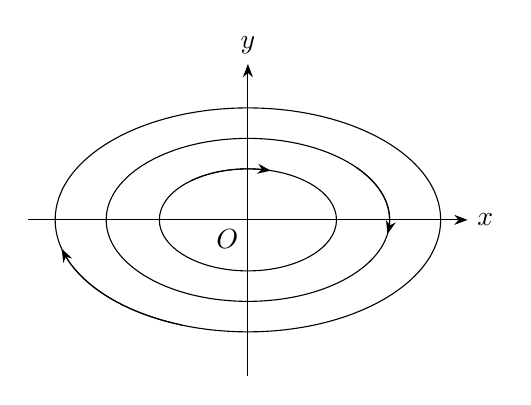
\begin{tikzpicture}[scale=0.9,>=Stealth]
			\draw[->] (-3.1,0)--(3.1,0) node[right] {$x$};
			\draw[->] (0,-2.2)--(0,2.2) node[above] {$y$};
			\node[below left] at (0,0) {$O$};
			\draw (0,0) ellipse (1.25 and 0.72);
			\draw (0,0) ellipse (2.00 and 1.15);
			\draw (0,0) ellipse (2.72 and 1.58);
			\draw[->] plot[domain=130:75,samples=20]
				({1.25*cos(\x)},{0.72*sin(\x)});
			\draw[->] plot[domain=40:-10,samples=20]
				({2*cos(\x)},{1.15*sin(\x)});
			\draw[->] plot[domain=-110:-165,samples=20]
				({2.72*cos(\x)},{1.58*sin(\x)});
		\end{tikzpicture}

		\small $k>0$ 时的相图
	\end{minipage}
	\hfill
	\begin{minipage}{0.46\textwidth}
		\centering
		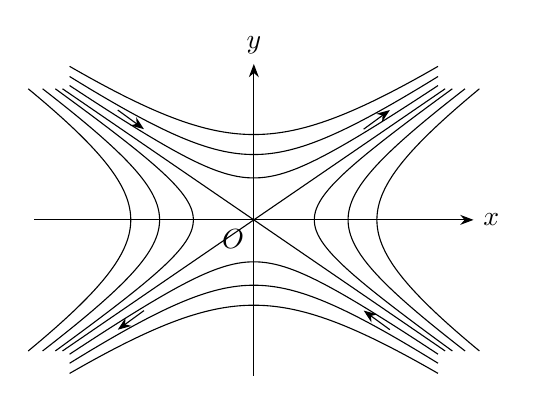
\begin{tikzpicture}[scale=0.9,>=Stealth]
			\draw[->] (-3.1,0)--(3.1,0) node[right] {$x$};
			\draw[->] (0,-2.2)--(0,2.2) node[above] {$y$};
			\node[below left] at (0,0) {$O$};
			\draw (-2.7,-1.85)--(2.7,1.85);
			\draw (-2.7,1.85)--(2.7,-1.85);
			\foreach \a in {0.35,0.85,1.45}{
				\draw plot[domain=-2.6:2.6,samples=80]
					(\x,{sqrt(0.48*\x*\x+\a)});
				\draw plot[domain=-2.6:2.6,samples=80]
					(\x,{-sqrt(0.48*\x*\x+\a)});
				\draw plot[domain=-1.85:1.85,samples=80]
					({sqrt(2.08*\x*\x+2.08*\a)},\x);
				\draw plot[domain=-1.85:1.85,samples=80]
					({-sqrt(2.08*\x*\x+2.08*\a)},\x);
			}
			\draw[->] (1.55,1.28)--(1.92,1.55);
			\draw[->] (-1.92,1.55)--(-1.55,1.28);
			\draw[->] (1.92,-1.55)--(1.55,-1.28);
			\draw[->] (-1.55,-1.28)--(-1.92,-1.55);
		\end{tikzpicture}

		\small $k<0$ 时的相图
	\end{minipage}
\end{figure}

进一步看，
\[
	\dfrac{m}{2}y^2
	\qquad\text{与}\qquad
	\dfrac{k}{2}x^2
\]
分别表示振子的动能与势能，所以 $H(x,y)$ 是系统的总机械能。
关系 $H(x,y)=C$ 表明沿任意一条轨道总机械能恒定不变，因而称该系统为
\textbf{保守系统}。它也是一个平面 Hamilton 系统，其运动轨道位于能量等位线上。
特别地，当 $k>0$ 时，相图中的闭轨道说明弹簧振子的自由振动是周期运动。

上面的方程是更一般的 Newton 系统
\[
	\dfrac{\dd^2x}{\dd t^2}+g(x)=0
\]
的特殊情形。仍令 $y=\dfrac{\dd x}{\dd t}$，方程可化为
\[
	y\,\dd y+g(x)\,\dd x=0.
\]
它具有总机械能
\[
	H(x,y)=\dfrac{1}{2}y^2+G(x),
	\qquad
	G(x)=\int_0^x g(s)\,\dd s.
\]
因此其积分曲线为
\[
	H(x,y)=C.
\]
由
\[
	y=\pm\sqrt{2\bigl(C-G(x)\bigr)}
\]
可知，$x(t)$ 可通过求解变量分离方程
\[
	\dfrac{\dd x}{\dd t}
	=\pm\sqrt{2\bigl(C-G(x)\bigr)}
\]
得到。

\subsection*{四、Riccati 方程}

\begin{definition}\label{def:Riccati方程}
	Riccati 方程是一类右端关于未知函数为二次多项式的一阶微分方程，写成
\[
	\dfrac{\dd x}{\dd t}
	=a(t)x^2+b(t)x+c(t),
\]
其中 $a,b,c$ 在区间 $I$ 上连续，且 $a(t)\neq 0$。
\end{definition}
若已知一个特解
$\phi(t)$，作变换
\[
	y=x-\phi(t),
\]
便可将原方程化为 Bernoulli 方程
\[
	\dfrac{\dd y}{\dd t}
	=\bigl(2a(t)\phi(t)+b(t)\bigr)y+a(t)y^2,
\]
从而用初等积分法求出通解。

下面考虑形式较为具体的 Riccati 方程
\[
	\dfrac{\dd x}{\dd t}=-x^2+ct^m,
\]
其中 $c$ 为常数，且 $t\neq 0$、$x\neq 0$。当 $m=0$ 时，该方程已经是
变量分离方程；当 $m=-2$ 时，作变换 $y=tx$，可化为
\[
	\dfrac{\dd y}{\dd t}
	=\dfrac{-y^2+y+c}{t},
\]
仍是变量分离方程。

当
\[
	m=\dfrac{-4k}{2k+1}
\]
时，通过变换
\[
	t=\tau^{-\dfrac{1}{m+1}},
	\qquad
	x=\left(\dfrac{c}{m+1}\right)
	\dfrac{1}{\tau-y\tau^2},
\]
原方程仍可化为同一类型
\[
	\dfrac{\dd y}{\dd\tau}
	=-y^2+c'\tau^n,
\]
其中
\[
	c'=\dfrac{c}{(m+1)^2},
	\qquad
	n=\dfrac{-4(k-1)}{2(k-1)+1}.
\]
重复上述过程 $k$ 次后，指数便降为零，从而得到变量分离方程。类似地，
当
\[
	m=\dfrac{-4k}{2k-1}
\]
时也可作同样的逐次化简。因此
\[
	m=0,\ -2,\ \dfrac{-4k}{2k\pm 1},
	\qquad k=1,2,\ldots
\]
是该 Riccati 方程能够用初等积分法求解的充分条件。Liouville 于 1841 年证明，
这一条件也是必要的。

这个例子说明，并非所有微分方程都能用初等积分法写出通解，即使方程的形式
看起来很简单也是如此。因此，在解析求解之外，还需要从方程本身出发研究解的
存在性、唯一性、周期性、有界性与稳定性等性质。

\setchapterimage{figure/Chapter3封面图}
\setchapterintro{}
\chapter{线性方程}\label{chap:线性方程}

考虑微分方程组
\[
	\dfrac{\dd \vect{x}}{\dd t}=\vect{f}(\vect{x}),
\]
其中 $\vect{x},\vect{f}\in\R^n$。若函数 $\vect{f}(\vect{x})$ 在
$\vect{x}=\vect{x}_0$ 处具有 Taylor 展开
\[
	\vect{f}(\vect{x})
	=\vect{f}(\vect{x}_0)
	+A(\vect{x}-\vect{x}_0)
	+\vect{R}(\vect{x}),
\]
其中 $\norm{\vect{R}(\vect{x})}$ 是
$\norm{\vect{x}-\vect{x}_0}$ 的高阶无穷小，$A$ 为 $n\times n$ 阶矩阵，
则在 $\vect{x}=\vect{x}_0$ 附近，可以用线性部分
\[
	\vect{f}(\vect{x}_0)+A(\vect{x}-\vect{x}_0)
\]
近似 $\vect{f}(\vect{x})$。因此，原方程组在 $\vect{x}_0$ 附近的解可由线性方程组
\[
	\dfrac{\dd \vect{x}}{\dd t}
	=\vect{f}(\vect{x}_0)+A(\vect{x}-\vect{x}_0)
\]
的解来近似。从这个意义上说，研究线性微分方程及线性微分方程组，
是进一步研究一般非线性微分方程及微分方程组的基础。

\section{存在性与唯一性}\label{sec:线性方程组的存在性与唯一性}

考虑含 $n$ 个未知函数的一阶线性微分方程组
\[
	\begin{cases}
		\dfrac{\dd x_1}{\dd t}
		=a_{11}(t)x_1+a_{12}(t)x_2+\cdots+a_{1n}(t)x_n+f_1(t),\\
		\dfrac{\dd x_2}{\dd t}
		=a_{21}(t)x_1+a_{22}(t)x_2+\cdots+a_{2n}(t)x_n+f_2(t),\\
		\hspace{4.5cm}\vdots\\
		\dfrac{\dd x_n}{\dd t}
		=a_{n1}(t)x_1+a_{n2}(t)x_2+\cdots+a_{nn}(t)x_n+f_n(t).
	\end{cases}
\]
其中已知函数 $a_{ij}(t)$、$f_i(t)$（$i,j=1,2,\ldots,n$）都是区间
$[\alpha,\beta]$ 上的连续函数。令
\[
	A(t)=
	\begin{pmatrix}
		a_{11}(t) & \cdots & a_{1n}(t)\\
		a_{21}(t) & \cdots & a_{2n}(t)\\
		\vdots    & \ddots & \vdots\\
		a_{n1}(t) & \cdots & a_{nn}(t)
	\end{pmatrix},
	\qquad
	\vect{f}(t)=
	\begin{pmatrix}
		f_1(t)\\
		f_2(t)\\
		\vdots\\
		f_n(t)
	\end{pmatrix},
	\qquad
	\vect{x}=
	\begin{pmatrix}
		x_1\\
		x_2\\
		\vdots\\
		x_n
	\end{pmatrix}.
\]
\begin{definition}\label{def:齐次与非齐次线性方程组}
	上述方程组可写成矩阵形式
\[
	\dfrac{\dd \vect{x}}{\dd t}
	=A(t)\vect{x}+\vect{f}(t).
\]
当 $\vect{f}(t)\equiv\boldsymbol{0}$ 时，称该方程组为\textbf{齐次线性方程组}；
否则称为\textbf{非齐次线性方程组}。

\end{definition}
\begin{theorem}\label{thm:线性方程组的存在唯一性}
	设 $A(t)$ 是区间 $[\alpha,\beta]$ 上的 $n\times n$ 阶连续矩阵函数，
	$\vect{f}(t)$ 是该区间上的 $n$ 维连续列向量函数。则对任意
	$t_0\in[\alpha,\beta]$ 及任意常向量 $\vect{x}^{\,0}\in\R^n$，
	初值问题
	\[
		\dfrac{\dd \vect{x}}{\dd t}
		=A(t)\vect{x}+\vect{f}(t),
		\qquad
		\vect{x}(t_0)=\vect{x}^{\,0}
	\]
	在整个区间 $[\alpha,\beta]$ 上存在唯一解。
\end{theorem}

为证明这一定理，先介绍矩阵函数的一些基本性质。矩阵函数的加法、乘法
与常数矩阵相同。若
\[
	A(t)=\bigl(a_{ij}(t)\bigr),
\]
且每个元素 $a_{ij}(t)$ 都是连续函数或可微函数，则分别称 $A(t)$ 为
连续矩阵函数或可微矩阵函数。在可微的情形下，
\[
	\dfrac{\dd A(t)}{\dd t}
	=\left(\dfrac{\dd a_{ij}(t)}{\dd t}\right).
\]
矩阵函数的导数满足
\[
	\dfrac{\dd}{\dd t}\bigl(A_1(t)+A_2(t)\bigr)
	=\dfrac{\dd A_1(t)}{\dd t}
	+\dfrac{\dd A_2(t)}{\dd t},
\]
\[
	\dfrac{\dd}{\dd t}\bigl(A_1(t)A_2(t)\bigr)
	=\dfrac{\dd A_1(t)}{\dd t}A_2(t)
	+A_1(t)\dfrac{\dd A_2(t)}{\dd t}.
\]

若 $A(t)=\bigl(a_{ij}(t)\bigr)$ 的每个元素在 $[\alpha,\beta]$ 上可积，
则称 $A(t)$ 在该区间上可积，并定义
\[
	\int_\alpha^\beta A(t)\,\dd t
	=\left(\int_\alpha^\beta a_{ij}(t)\,\dd t\right).
\]

\begin{definition}\label{def:矩阵与向量的范数}
	对 $n\times n$ 阶矩阵 $A=(a_{ij})$ 与 $n$ 维向量
	$\vect{x}=(x_1,\ldots,x_n)^{\mathsf T}$，分别定义范数
	\[
		\norm{A}=\sum_{i,j=1}^{n}|a_{ij}|,
		\qquad
		\norm{\vect{x}}=\sum_{i=1}^{n}|x_i|.
	\]
\end{definition}

对任意 $n\times n$ 阶矩阵 $A_1,A_2$、$n$ 维向量
$\vect{x}_1,\vect{x}_2$ 及标量 $\gamma\in\R$（或 $\C$），有
\[
	\norm{A_1+A_2}\leqslant\norm{A_1}+\norm{A_2},
	\qquad
	\norm{\vect{x}_1+\vect{x}_2}
	\leqslant\norm{\vect{x}_1}+\norm{\vect{x}_2},
\]
\[
	\norm{\gamma A}=|\gamma|\norm{A},
	\qquad
	\norm{\gamma\vect{x}}=|\gamma|\norm{\vect{x}},
\]
\[
	\norm{A_1A_2}\leqslant\norm{A_1}\norm{A_2},
	\qquad
	\norm{A\vect{x}}\leqslant\norm{A}\norm{\vect{x}},
\]
以及
\[
	\norm{\int_\alpha^\beta A(t)\,\dd t}
	\leqslant
	\int_\alpha^\beta\norm{A(t)}\,\dd t.
\]

\begin{definition}\label{def:矩阵函数序列的收敛}
	设
	\[
		A_k(t)=\bigl(a_{ij}^{(k)}(t)\bigr)
	\]
	是 $n\times n$ 阶矩阵函数序列。若对所有 $i,j=1,2,\ldots,n$，
	函数序列 $\{a_{ij}^{(k)}(t)\}$ 都在 $[\alpha,\beta]$ 上收敛或一致收敛，
	则称 $\{A_k(t)\}$ 在该区间上收敛或一致收敛。

	类似地，矩阵函数项级数
	\[
		\sum_{k=1}^{\infty}A_k(t)
	\]
	在 $[\alpha,\beta]$ 上收敛或一致收敛，是指对任意
	$i,j=1,2,\ldots,n$，函数项级数
	\[
		\sum_{k=1}^{\infty}a_{ij}^{(k)}(t)
	\]
	在该区间上收敛或一致收敛。
\end{definition}

\begin{proof}[定理的证明]
	\textbf{第一步：化为等价积分方程。}
	初值问题等价于
	\[
		\vect{x}(t)
		=\vect{x}^{\,0}
		+\int_{t_0}^{t}
		\bigl(A(\tau)\vect{x}(\tau)+\vect{f}(\tau)\bigr)\,\dd\tau.
	\]
	事实上，微分方程的解积分后满足上式；反之，上式右端连续可微，
	对 $t$ 求导并令 $t=t_0$，即可恢复微分方程和初值条件。

	\textbf{第二步：构造逐次逼近序列。}
	令
	\[
		\vect{x}_0(t)\equiv\vect{x}^{\,0},
	\]
	并递归定义
	\[
		\vect{x}_k(t)
		=\vect{x}^{\,0}
		+\int_{t_0}^{t}
		\bigl(A(\tau)\vect{x}_{k-1}(\tau)
		+\vect{f}(\tau)\bigr)\,\dd\tau,
		\qquad k=1,2,\ldots.
	\]
	由连续函数的积分性质可知，每个 $\vect{x}_k(t)$ 都在
	$[\alpha,\beta]$ 上有定义且连续。

	\textbf{第三步：证明逐次逼近序列一致收敛。}
	由于 $A(t)$ 与 $\vect{f}(t)$ 在闭区间上连续，存在常数 $M>0$，使
	\[
		\norm{A(t)}\leqslant M,
		\qquad
		\norm{\vect{f}(t)}\leqslant M,
		\qquad \alpha\leqslant t\leqslant\beta.
	\]
	由递推式归纳可得，对任意正整数 $j$，
	\[
		\norm{\vect{x}_j(t)-\vect{x}_{j-1}(t)}
		\leqslant
		\bigl(\norm{\vect{x}^{\,0}}+1\bigr)
		\dfrac{M^j}{j!}|t-t_0|^j.
	\]
	证明时，$j=1$ 的情形直接由积分估计得到；若对 $j=m$ 成立，则
	\[
		\begin{aligned}
		\norm{\vect{x}_{m+1}(t)-\vect{x}_m(t)}
		&\leqslant
		\left|
		\int_{t_0}^{t}
		\norm{A(\tau)}
		\norm{\vect{x}_m(\tau)-\vect{x}_{m-1}(\tau)}
		\,\dd\tau
		\right|\\
		&\leqslant
		M\bigl(\norm{\vect{x}^{\,0}}+1\bigr)
		\dfrac{M^m}{m!}
		\left|
		\int_{t_0}^{t}|\tau-t_0|^m\,\dd\tau
		\right|\\
		&=
		\bigl(\norm{\vect{x}^{\,0}}+1\bigr)
		\dfrac{M^{m+1}}{(m+1)!}|t-t_0|^{m+1}.
		\end{aligned}
	\]
	又因为级数
	\[
		\sum_{j=1}^{\infty}\dfrac{M^j}{j!}|t-t_0|^j
	\]
	在 $[\alpha,\beta]$ 上一致收敛，所以
	\[
		\vect{x}_0(t)
		+\sum_{j=1}^{\infty}
		\bigl(\vect{x}_j(t)-\vect{x}_{j-1}(t)\bigr)
	\]
	一致收敛。它的前 $k$ 项之和正是 $\vect{x}_k(t)$，故
	$\{\vect{x}_k(t)\}$ 一致收敛。

	\textbf{第四步：验证极限函数是解。}
	设
	\[
		\lim_{k\to\infty}\vect{x}_k(t)=\vect{x}(t).
	\]
	连续函数序列的一致极限仍连续。对递推式两端令 $k\to\infty$，
	并利用一致收敛性将极限移入积分号内，得到
	\[
		\vect{x}(t)
		=\vect{x}^{\,0}
		+\int_{t_0}^{t}
		\bigl(A(\tau)\vect{x}(\tau)+\vect{f}(\tau)\bigr)\,\dd\tau.
	\]
	因此 $\vect{x}(t)$ 满足等价积分方程，从而是原初值问题的解。

	\textbf{第五步：证明解的唯一性。}
	设 $\widetilde{\vect{x}}(t)$ 是同一区间上的另一个解，并令
	\[
		\vect{y}(t)=\vect{x}(t)-\widetilde{\vect{x}}(t).
	\]
	则
	\[
		\vect{y}(t)
		=\int_{t_0}^{t}A(\tau)\vect{y}(\tau)\,\dd\tau.
	\]
	取 $L>0$ 使 $\norm{\vect{y}(t)}\leqslant L$。与前面的估计相同，
	对任意正整数 $k$ 都有
	\[
		\norm{\vect{y}(t)}
		\leqslant
		\dfrac{LM^k}{k!}|t-t_0|^k,
		\qquad \alpha\leqslant t\leqslant\beta.
	\]
	令 $k\to\infty$，右端趋于零，故
	$\vect{y}(t)\equiv\boldsymbol{0}$，即
	$\vect{x}(t)\equiv\widetilde{\vect{x}}(t)$。
\end{proof}

\section{齐次线性方程组的通解结构}\label{sec:齐次线性方程组的通解结构}

本节讨论齐次线性微分方程组
\[
	\dfrac{\dd\vect{x}}{\dd t}=A(t)\vect{x},
\]
其中 $A(t)$ 是区间 $[\alpha,\beta]$ 上的 $n\times n$ 阶连续矩阵函数。

\begin{theorem}\label{thm:齐次线性方程组的解空间}
	如果 $\vect{x}_1(t)$ 和 $\vect{x}_2(t)$ 是上述齐次线性方程组的两个解，则
	\[
		\vect{x}(t)
		=C_1\vect{x}_1(t)+C_2\vect{x}_2(t)
	\]
	也是该方程组的解，其中 $C_1,C_2$ 为任意常数。并且，方程组全部解的集合
	$\mathcal{S}$ 是一个 $n$ 维线性空间。
\end{theorem}

\begin{proof}
	由求导的线性性可直接验证任意两个解的线性组合仍是解。

	任取 $\R^n$（或 $\C^n$）中的一组基
	$\vect{x}_1^{\,0},\ldots,\vect{x}_n^{\,0}$，并固定
	$t_0\in[\alpha,\beta]$。由定理~\ref{thm:线性方程组的存在唯一性}，对每个
	$k=1,\ldots,n$，存在唯一解 $\vect{x}_k(t)$ 满足
	\[
		\vect{x}_k(t_0)=\vect{x}_k^{\,0}.
	\]
	若
	\[
		\sum_{k=1}^{n}C_k\vect{x}_k(t)\equiv\boldsymbol{0},
	\]
	在 $t=t_0$ 处取值得
	\[
		\sum_{k=1}^{n}C_k\vect{x}_k^{\,0}=\boldsymbol{0}.
	\]
	由于初始向量线性无关，必有 $C_1=\cdots=C_n=0$，故
	$\vect{x}_1(t),\ldots,\vect{x}_n(t)$ 线性无关。

	另一方面，任取方程组的解 $\vect{x}(t)$，可将其初值唯一地写成
	\[
		\vect{x}(t_0)
		=\sum_{k=1}^{n}C_k\vect{x}_k^{\,0}.
	\]
	由叠加原理，$\sum\limits_{k=1}^{n}C_k\vect{x}_k(t)$ 也是方程组的解，
	并与 $\vect{x}(t)$ 具有相同初值。再由唯一性，
	\[
		\vect{x}(t)
		=\sum_{k=1}^{n}C_k\vect{x}_k(t).
	\]
	因此这 $n$ 个解构成 $\mathcal{S}$ 的一组基，故
	$\dim\mathcal{S}=n$。
\end{proof}

上述证明说明：固定 $t_0$ 后，每个初始向量
$\vect{x}^{\,0}\in\R^n$（或 $\C^n$）都唯一对应方程组的一个解。
映射
\[
	\sigma:\vect{x}^{\,0}\longmapsto\vect{x}(t)
\]
给出了初始向量空间与解空间 $\mathcal{S}$ 之间的线性同构。

\begin{definition}\label{def:基本解组}
	齐次线性方程组的任意 $n$ 个线性无关解
	\[
		\bigl\{\vect{x}_k(t):k=1,2,\ldots,n\bigr\}
	\]
	称为该方程组的一个\textbf{基本解组}。
\end{definition}

基本解组一般不唯一。一旦得到一个基本解组，方程组的通解便可写成
\[
	\vect{x}(t)
	=\sum_{k=1}^{n}C_k\vect{x}_k(t),
\]
其中 $C_1,\ldots,C_n$ 为任意常数。因此，求齐次线性方程组的通解，
可归结为求它的 $n$ 个线性无关特解。

设
\[
	\vect{x}_k(t)=
	\begin{pmatrix}
		x_{1k}(t)\\
		x_{2k}(t)\\
		\vdots\\
		x_{nk}(t)
	\end{pmatrix},
	\qquad k=1,2,\ldots,n,
\]
是方程组的 $n$ 个解。

\begin{definition}\label{def:解矩阵与Wronski行列式}
	由这些解作为列向量构成的矩阵
	\[
		X(t)
		=\bigl(\vect{x}_1(t),\vect{x}_2(t),\ldots,\vect{x}_n(t)\bigr)
		=
		\begin{pmatrix}
			x_{11}(t) & x_{12}(t) & \cdots & x_{1n}(t)\\
			x_{21}(t) & x_{22}(t) & \cdots & x_{2n}(t)\\
			\vdots    & \vdots    & \ddots & \vdots\\
			x_{n1}(t) & x_{n2}(t) & \cdots & x_{nn}(t)
		\end{pmatrix}
	\]
	称为该方程组的一个\textbf{解矩阵}，其行列式
	\[
		W(t)=\det X(t)
	\]
	称为这组解的 \textbf{Wronski 行列式}。
\end{definition}

由线性代数可知，若一般的 $n$ 个向量函数线性相关，则其 Wronski
行列式恒为零。对于齐次线性方程组的解，反命题也成立。

\begin{lemma}\label{lem:行列式的导数}
	设 $B(t)$ 是可微的 $n\times n$ 阶矩阵，其第 $k$ 行为
	$\vect{r}_k(t)$。则
	\[
		\dfrac{\dd}{\dd t}\det B(t)
		=
		\sum_{k=1}^{n}
		\det
		\begin{pmatrix}
			\vect{r}_1(t)\\
			\vdots\\
			\vect{r}_{k-1}(t)\\
			\dfrac{\dd\vect{r}_k(t)}{\dd t}\\
			\vect{r}_{k+1}(t)\\
			\vdots\\
			\vect{r}_n(t)
		\end{pmatrix}.
	\]
\end{lemma}

\begin{proof}
	将行列式写成 Leibniz 展开式并逐项求导；乘积求导所得的第 $k$ 组项，
	正好组成把原行列式第 $k$ 行换成其导数后的行列式。
\end{proof}

\begin{theorem}\label{thm:Wronski判别与Liouville公式}
	齐次线性方程组的解组
	$\{\vect{x}_k(t):k=1,2,\ldots,n\}$ 线性无关的充分必要条件是：
	其 Wronski 行列式在某点 $t_0\in[\alpha,\beta]$ 处不为零。
	并且
	\[
		\det X(t)
		=\det X(t_0)
		\exp\left(
		\int_{t_0}^{t}\operatorname{tr}A(\tau)\,\dd\tau
		\right),
	\]
	其中
	\[
		\operatorname{tr}A(t)=\sum_{k=1}^{n}a_{kk}(t)
	\]
	是矩阵 $A(t)$ 的迹。上述等式称为\textbf{Liouville 公式}。
\end{theorem}

\begin{proof}
	由于 $X'(t)=A(t)X(t)$，解矩阵的第 $k$ 行导数可写成
	\[
		\dfrac{\dd\vect{r}_k(t)}{\dd t}
		=\sum_{j=1}^{n}a_{kj}(t)\vect{r}_j(t).
	\]
	由引理~\ref{lem:行列式的导数}及行列式对各行的线性性，将第 $k$ 行导数代入后，
	当 $j\neq k$ 时行列式含有两个相同的行，因而等于零；仅
	$j=k$ 的一项保留下来。因此
	\[
		\begin{aligned}
		\dfrac{\dd}{\dd t}\det X(t)
		&=\sum_{k=1}^{n}a_{kk}(t)\det X(t)\\
		&=\operatorname{tr}A(t)\det X(t).
		\end{aligned}
	\]
	解这个一阶线性方程便得到 Liouville 公式。

	若 $\det X(t_0)\neq 0$，则
	$\vect{x}_1(t_0),\ldots,\vect{x}_n(t_0)$ 线性无关，从而这些解线性无关。
	反之，若 $\det X(t_0)=0$，则存在不全为零的常数
	$C_1,\ldots,C_n$，使
	\[
		\sum_{k=1}^{n}C_k\vect{x}_k(t_0)=\boldsymbol{0}.
	\]
	该线性组合是齐次方程组满足零初值的解，由唯一性只能恒为零，
	故这组解线性相关。充分必要性得证。
\end{proof}

由 Liouville 公式可知，齐次线性方程组的解矩阵行列式或者恒为零，
或者在整个区间上处处不为零。这个结论只适用于由同一个齐次线性方程组的
解构成的矩阵。一般向量函数没有这种性质，例如
\[
	\begin{pmatrix}
		t\\
		0
	\end{pmatrix},
	\qquad
	\begin{pmatrix}
		t^2\\
		0
	\end{pmatrix}
\]
作为向量函数是线性无关的，但它们的 Wronski 行列式恒等于零。

\begin{definition}\label{def:基本解矩阵与标准解矩阵}
	当解组 $\{\vect{x}_k(t):k=1,2,\ldots,n\}$ 是一个基本解组时，
	相应的解矩阵 $X(t)$ 称为方程组的一个\textbf{基本解矩阵}。
	特别地，若在某点 $t_0$ 有
	\[
		X(t_0)=I,
	\]
	则称 $X(t)$ 为以 $t_0$ 为基点的\textbf{标准解矩阵}。
\end{definition}

若 $X(t)$ 是一个基本解矩阵，则齐次方程组的任一解都可表示为
\[
	\vect{x}(t)=X(t)\vect{c},
\]
其中 $\vect{c}$ 为常向量；反之，对任意常向量 $\vect{c}$，
$X(t)\vect{c}$ 都是方程组的解。

若再给定初值条件
\[
	\vect{x}(t_0)=\vect{x}^{\,0},
\]
则
\[
	\vect{c}=X^{-1}(t_0)\vect{x}^{\,0},
\]
从而初值问题的解为
\[
	\vect{x}(t)=X(t,t_0)\vect{x}^{\,0},
\]
其中
\[
	X(t,t_0):=X(t)X^{-1}(t_0)
\]
是以 $t_0$ 为基点的标准解矩阵。

\section{非齐次线性方程组的通解}\label{sec:非齐次线性方程组的通解}

本节利用第~\ref{sec:齐次线性方程组的通解结构}节的结果，进一步讨论非齐次线性方程组
\[
	\dfrac{\dd\vect{x}}{\dd t}=A(t)\vect{x}+\vect{f}(t)
\]
的解的结构，其中 $A(t)$ 是区间 $[\alpha,\beta]$ 上的 $n\times n$ 阶连续矩阵函数，
$\vect{f}(t)$ 是 $[\alpha,\beta]$ 上的 $n$ 维连续列向量函数。当
$\vect{f}(t)\equiv\boldsymbol{0}$ 时，方程组化为
\[
	\dfrac{\dd\vect{x}}{\dd t}=A(t)\vect{x},
\]
称为与原方程组相应的齐次线性方程组。

容易验证，若 $\vect{x}_1^{\,*}(t)$ 和 $\vect{x}_2^{\,*}(t)$ 是非齐次方程组的两个解，
则 $\vect{x}_1^{\,*}(t)-\vect{x}_2^{\,*}(t)$ 是相应齐次方程组的解；反之，
若 $\vect{x}^{\,*}(t)$ 和 $\vect{x}(t)$ 分别是非齐次方程组和相应齐次方程组的解，
则 $\vect{x}^{\,*}(t)+\vect{x}(t)$ 仍是非齐次方程组的解。

\begin{theorem}\label{thm:非齐次线性方程组的通解结构}
	若 $\vect{x}^{\,*}(t)$ 是非齐次线性方程组的一个解，$X(t)$ 是相应齐次线性方程组的
	基本解矩阵，则非齐次线性方程组的通解为
	\[
		\vect{x}(t)=X(t)\vect{c}+\vect{x}^{\,*}(t),
	\]
	其中 $\vect{c}$ 是任意 $n$ 维常向量。
\end{theorem}

\begin{proof}
	若 $\vect{x}(t)$ 是非齐次方程组的任一解，则
	$\vect{x}(t)-\vect{x}^{\,*}(t)$ 是相应齐次方程组的解，故存在常向量
	$\vect{c}$，使得
	\[
		\vect{x}(t)-\vect{x}^{\,*}(t)=X(t)\vect{c}.
	\]
	反之，将 $X(t)\vect{c}+\vect{x}^{\,*}(t)$ 代入原方程组即可验证它是解。
\end{proof}

\begin{theorem}\label{thm:常数变易公式}
	设 $X(t)$ 是相应齐次线性方程组在 $[\alpha,\beta]$ 上的基本解矩阵，
	则非齐次线性方程组的通解为
	\[
		\vect{x}(t)
		=X(t)\vect{c}
		+X(t)\int_{t_0}^{t}X^{-1}(\tau)\vect{f}(\tau)\,\dd\tau,
	\]
	其中 $\vect{c}$ 为任意 $n$ 维常向量。满足初值条件
	\[
		\vect{x}(t_0)=\vect{x}^{\,0}
	\]
	的解为
	\[
		\vect{x}(t)
		=X(t,t_0)\vect{x}^{\,0}
		+\int_{t_0}^{t}X(t,\tau)\vect{f}(\tau)\,\dd\tau,
	\]
	其中 $t,t_0\in[\alpha,\beta]$，并且
	\[
		X(t,t_0)=X(t)X^{-1}(t_0).
	\]
\end{theorem}

上述通解表达式与初值问题的解表达式统称为\textbf{常数变易公式}。

\begin{proof}
	相应齐次线性方程组的通解为 $X(t)\vect{c}$。将常向量 $\vect{c}$ 变易为
	待定向量函数 $\vect{c}(t)$，设非齐次方程组有形如
	\[
		\vect{x}^{\,*}(t)=X(t)\vect{c}(t)
	\]
	的特解。代入非齐次方程组，得到
	\[
		\dfrac{\dd X(t)}{\dd t}\vect{c}(t)
		+X(t)\dfrac{\dd\vect{c}(t)}{\dd t}
		=A(t)X(t)\vect{c}(t)+\vect{f}(t).
	\]
	由于 $X(t)$ 是齐次方程组的解矩阵，故
	\[
		\dfrac{\dd X(t)}{\dd t}=A(t)X(t),
	\]
	从而
	\[
		X(t)\dfrac{\dd\vect{c}(t)}{\dd t}=\vect{f}(t).
	\]
	基本解矩阵 $X(t)$ 可逆，因此
	\[
		\dfrac{\dd\vect{c}(t)}{\dd t}=X^{-1}(t)\vect{f}(t).
	\]
	两端积分可得
	\[
		\vect{c}(t)
		=\vect{c}^{\,0}
		+\int_{t_0}^{t}X^{-1}(\tau)\vect{f}(\tau)\,\dd\tau,
	\]
	其中 $\vect{c}^{\,0}$ 为常向量。特别地，取 $\vect{c}^{\,0}=\boldsymbol{0}$，
	便得到一个特解
	\[
		\vect{x}^{\,*}(t)
		=X(t)\int_{t_0}^{t}X^{-1}(\tau)\vect{f}(\tau)\,\dd\tau.
	\]
	结合定理~\ref{thm:非齐次线性方程组的通解结构}，便得到定理中的通解表达式。

	再由 $X(t,\tau)=X(t)X^{-1}(\tau)$，并令初值为
	$\vect{x}(t_0)=\vect{x}^{\,0}$，即可得到定理中的初值解表达式。
\end{proof}

虽然定理~\ref{thm:Wronski判别与Liouville公式}已经给出了判别一个解矩阵是否为基本解矩阵的方法，但一般来说，
求齐次线性微分方程组的基本解矩阵仍不是容易的事。对于常系数矩阵
$A(t)=A$ 的情形，将在下一章讨论其基本解矩阵的求法。

\subsection*{集中脉冲与影响函数}
\phantomsection\label{sec:green-response}
由定理~\ref{thm:常数变易公式}，非齐次方程的解可以表示为齐次方程的解与一个积分之和。对于标量方程 $y'=a(t)y+f(t)$，这个积分表示非齐次项对解的影响。下面先考察非齐次项集中在一个时刻附近的情形。


\begin{definition}[光滑函数、支撑与测试函数]\label{def:support-test}
在开集 $U\subset\R^n$ 上，$C^r(U)$ 表示所有总阶数不超过 $r$ 的偏导数都存在且连续的函数；
$C^\infty(U)$ 表示任意阶偏导数都存在且连续的函数，亦称光滑函数。
函数 $f$ 的支撑（也称支集）定义为相对于 $U$ 的闭包
\[
 \operatorname{supp}f=\overline{\{x\in U:f(x)\ne0\}}^{\,U}.
\]
若这个闭集是 $U$ 中的紧集，称 $f$ 有紧支撑。
光滑紧支撑函数称为测试函数，全体记为 $C_c^\infty(U)$。
在有限维空间内，本书的光滑向量函数指各分量均光滑。
\end{definition}
\begin{example}[光滑凸起与截断]\label{ex:smooth-cutoff}
令
\[
 b(s)=\begin{cases}e^{-1/s},&s>0,\\0,&s\leq0,\end{cases}
 \qquad \chi(x)=\frac{b(4-|x|^2)}{b(4-|x|^2)+b(|x|^2-1)}.
\]
每阶右导数都是 $e^{-1/s}$ 乘以 $s^{-1}$ 的多项式，在 $s\downarrow0$ 时趋于零，
所以 $b$ 光滑。分母处处为正，故 $\chi$ 光滑，且 $0\leq\chi\leq1$，
在 $|x|\leq1$ 时为 1，在 $|x|\geq2$ 时为零。$\chi(x/r)$ 称尺度为 $r$ 的截断函数。
此外，$b(1-|x|^2)$ 是非负、非零且紧支撑的光滑函数；除以其正积分即可使积分为 1。
\end{example}
\begin{definition}[单位集中质量的记号]
对连续函数 $f$，记 $\langle\delta_\xi,f\rangle=f(\xi)$。
这表示对函数取值的线性规则，不表示一个通常的函数 $\delta_\xi(s)$。
光滑函数序列 $h_N$ 趋向 $\delta_\xi$，在这里是指
\[
 \int h_N(s)\psi(s)\,ds\longrightarrow\psi(\xi)
 \quad\text{对每个 }\psi\in C_c^\infty(\R)\text{ 成立}.
\]
下面将证明上述极限对在给定点附近连续的函数也成立。
\end{definition}

\begin{definition}[$\delta$ 型序列]
设 $h_N\geq0$ 为光滑函数，$\displaystyle\int_\R h_N(s)\,\dd s=1$，
且存在 $\varepsilon_N\downarrow0$，使 $h_N$ 在 $[-\varepsilon_N,\varepsilon_N]$ 外为零。
称 $(h_N)$ 为一个 $\delta$ 型序列。记号 $\delta$ 表示其对测试函数积分的极限，
不是一个处处有限的通常函数。
\end{definition}
\begin{lemma}
若 $f$ 在 $\xi$ 附近连续，则
\[
 \lim_{N\to\infty}\int_\R h_N(s-\xi)f(s)\,\dd s=f(\xi).
\]
\end{lemma}
\begin{proof}
因为脉冲非负且积分为 1，先把常数 $f(\xi)$ 写成
$f(\xi)\displaystyle\int h_N(s-\xi)\,ds$。于是
\begin{align*}
 \left|\int h_N(s-\xi)f(s)\,ds-f(\xi)\right|
 &=\left|\int h_N(s-\xi)(f(s)-f(\xi))\,ds\right|\\
 &\leq\sup_{|s-\xi|\leq\varepsilon_N}|f(s)-f(\xi)|
       \int h_N(s-\xi)\,ds\\
 &=\sup_{|s-\xi|\leq\varepsilon_N}|f(s)-f(\xi)|.
\end{align*}
由支集条件，被积函数在 $\xi$ 的小邻域外恒为零。
给定任意 $\eta>0$，连续性给出 $\delta>0$，使 $|s-\xi|<\delta$ 时
$|f(s)-f(\xi)|<\eta$。充分大的 $N$ 满足 $\varepsilon_N<\delta$，
所以上述差小于 $\eta$，极限成立。
\end{proof}

\begin{definition}[推迟影响函数]
对 $y'=a(t)y+f(t)$，给定零初值 $y(t_0)=0$。
在 $\xi>t_0$ 加入单位集中脉冲所产生的极限响应，称为在 $\xi$ 施加扰动的
\textbf{影响函数}，亦称推迟 Green 函数，记作 $G(t,\xi)$。
“推迟”表示扰动发生之前响应为零。
\end{definition}
\begin{theorem}
设 $a$ 连续，则在 $t\ne\xi$ 时
\[
 G(t,\xi)=
 \begin{cases}
 0,&t<\xi,\\
 \exp\displaystyle\int_\xi^t a(s)\,\dd s,&t>\xi.
 \end{cases}
\]
在 $t=\xi$ 处的右极限与左极限之差为 1。对连续 $f$ 和 $t\geq t_0$，
\[
 y(t)=\int_{t_0}^tG(t,\xi)f(\xi)\,\dd\xi
\]
是零初值问题的唯一解。
\end{theorem}
\begin{proof}
把 $f(t)$ 换成 $h_N(t-\xi)$。由本章已证的常数变易公式，响应为
\[
 y_N(t)=\int_{t_0}^t
 \exp\left(\int_s^t a(u)\,\dd u\right)h_N(s-\xi)\,\dd s.
\]
固定 $t<\xi$ 时，充分大的 $N$ 使积分区间与脉冲支集不相交，因此极限为零。
固定 $t>\xi$ 时，脉冲支集最终包含在积分区间内部，前一引理给出所述指数函数。
由 $a$ 连续，指数在 $t\downarrow\xi$ 时趋于 1，所以跳跃为 1。

最后的积分公式由常数变易公式直接得到。也可对该积分关于 $t$ 求导：对积分上限求导得 $f(t)$，
对被积函数求导后积分得 $a(t)y(t)$。在 $t=t_0$ 时积分为零，故满足初值条件。唯一性由
定理~\ref{thm:线性方程组的存在唯一性} 保证。
\end{proof}
\begin{remark}
边界点 $t=\xi$ 处的单点赋值不影响上式积分。
如果脉冲恰好位于初值时刻，应另外约定左右侧初值，不能把脉冲跨越的跳跃忽略。
对于向量方程，将指数函数换成矩阵 $X(t)X(s)^{-1}$，即可用同样的方法证明。
\end{remark}

图~\ref{fig:ode-tikz-pulse-green} 将光滑脉冲的集中过程与极限响应分开表示；空心点不指定 $t=\xi$ 处的单点取值。
\begin{center}
\begin{minipage}{0.96\linewidth}
\centering
% TikZ mathematical illustration; compiled with the main document.
\begin{tikzpicture}[>=Stealth,font=\small]
\begin{scope}[x=1.1cm,y=1cm]
 \draw[->,gray] (0,0)--(4,0) node[right]{$t$};
 \draw[->,gray] (.2,0)--(.2,3.2) node[above]{$h_N(t-\xi)$};
 \draw[gray,dashed] (2,0)--(2,3);
\draw[GreenMain,thick,domain=1.00100:2.99900,samples=90] plot (\x,{exp(1-1/(1-((\x-2)/1.0)^2))/(1.0*1.20690032)});
\draw[GoldMain,thick,domain=1.50050:2.49950,samples=90] plot (\x,{exp(1-1/(1-((\x-2)/0.5)^2))/(0.5*1.20690032)});
\draw[GreenDark,thick,domain=1.70030:2.29970,samples=90] plot (\x,{exp(1-1/(1-((\x-2)/0.3)^2))/(0.3*1.20690032)});

 \node[below] at (2,0){$\xi$};\node at (2,-.6){支集缩小，面积保持为 1};
\end{scope}
\begin{scope}[shift={(6.5,0)},x=1.1cm,y=1.8cm]
 \draw[->,gray] (0,0)--(4.4,0) node[right]{$t$};
 \draw[->,gray] (0,0)--(0,1.7) node[above]{$G(t,\xi)$};
 \draw[GreenMain,thick] (0,0)--(1,0);
 \draw[GreenMain,thick,domain=1:4,samples=65] plot (\x,{exp(-.7*(\x-1))});
 \draw[GoldMain,dashed] (1,0)--(1,1);
 \draw[fill=white,GreenMain] (1,0) circle(1.8pt);\draw[fill=white,GreenMain] (1,1) circle(1.8pt);
 \node[below] at (1,0){$\xi$};\node[left] at (0,1){$1$};
 \node at (2,-.34){$a(t)=-0.7$};
\end{scope}
\end{tikzpicture}
\captionof{figure}{左：单位面积光滑集中脉冲。右：$a=-0.7$ 时推迟影响函数在扰动时刻产生单位跳跃。}
\label{fig:ode-tikz-pulse-green}
\end{minipage}
\end{center}

\section{高阶线性方程}\label{sec:高阶线性方程}

$n$ 阶线性微分方程的一般形式为
\[
	\dfrac{\dd^n x}{\dd t^n}
	+a_1(t)\dfrac{\dd^{n-1}x}{\dd t^{n-1}}
	+\cdots+a_n(t)x=f(t),
\]
其中系数 $a_1(t),a_2(t),\ldots,a_n(t)$ 都在区间
$[\alpha,\beta]$ 上连续。当 $f(t)\equiv 0$ 时，
上述方程化为相应的齐次线性微分方程
\[
	\dfrac{\dd^n x}{\dd t^n}
	+a_1(t)\dfrac{\dd^{n-1}x}{\dd t^{n-1}}
	+\cdots+a_n(t)x=0.
\]

令
\[
	x_1=x,
	\qquad
	x_2=\dfrac{\dd x}{\dd t},
	\qquad\ldots\qquad
	x_n=\dfrac{\dd^{n-1}x}{\dd t^{n-1}},
\]
则原 $n$ 阶非齐次方程可化为一阶线性微分方程组
\[
	\dfrac{\dd\vect{x}}{\dd t}
	=A(t)\vect{x}+\vect{f}(t),
\]
其中
\[
	A(t)=
	\begin{pmatrix}
		0       & 1          & 0          & \cdots & 0\\
		0       & 0          & 1          & \cdots & 0\\
		\vdots  & \vdots     & \vdots     & \ddots & \vdots\\
		0       & 0          & 0          & \cdots & 1\\
		-a_n(t) & -a_{n-1}(t)& -a_{n-2}(t)& \cdots & -a_1(t)
	\end{pmatrix},
\]
\[
	\vect{f}(t)=
	\begin{pmatrix}
		0\\
		0\\
		\vdots\\
		0\\
		f(t)
	\end{pmatrix},
	\qquad
	\vect{x}=
	\begin{pmatrix}
		x_1\\
		x_2\\
		\vdots\\
		x_{n-1}\\
		x_n
	\end{pmatrix}.
\]

当 $f(t)\equiv 0$ 时，上述一阶方程组成为齐次线性微分方程组
\[
	\dfrac{\dd\vect{x}}{\dd t}=A(t)\vect{x}.
\]
显然，由原 $n$ 阶非齐次方程的任一解 $x=\phi(t)$，
可得到上述一阶方程组的一个解
\[
	\begin{pmatrix}
		\phi(t)\\
		\phi'(t)\\
		\vdots\\
		\phi^{(n-1)}(t)
	\end{pmatrix}.
\]
反之，上述一阶方程组任一解的第一个分量就是原 $n$ 阶非齐次方程的解。
特别地，满足初值条件
\[
	x(t_0)=x_0,
	\qquad
	x'(t_0)=x_0^{1},
	\qquad\ldots\qquad
	x^{(n-1)}(t_0)=x_0^{n-1}
\]
的解，由定理~\ref{thm:线性方程组的存在唯一性}知，在区间
$[\alpha,\beta]$ 上存在并且唯一。

\begin{definition}\label{def:高阶线性方程的Wronski行列式}
	设 $x_1(t),x_2(t),\ldots,x_n(t)$ 是上述 $n$ 阶齐次方程的 $n$ 个解，称
	\[
		W(t)=
		\begin{vmatrix}
			x_1(t) & x_2(t) & \cdots & x_n(t)\\
			x_1'(t) & x_2'(t) & \cdots & x_n'(t)\\
			\vdots & \vdots & \ddots & \vdots\\
			x_1^{(n-1)}(t) & x_2^{(n-1)}(t) & \cdots & x_n^{(n-1)}(t)
		\end{vmatrix}
	\]
	为解组 $\{x_k(t):k=1,2,\ldots,n\}$ 的 \textbf{Wronski 行列式}。
\end{definition}

\begin{definition}\label{def:高阶齐次线性方程的基本解组}
	上述 $n$ 阶齐次方程的任意 $n$ 个线性无关解的全体，
	称为该方程的一个\textbf{基本解组}。
\end{definition}

利用上述高阶方程与一阶方程组的对应关系，可以把前几节的结果直接推广到
高阶线性方程。

\begin{theorem}\label{thm:高阶齐次线性方程的通解}
	上述 $n$ 阶齐次线性微分方程在区间
	$[\alpha,\beta]$ 上存在 $n$ 个线性无关的解
	$x_1(t),x_2(t),\ldots,x_n(t)$，并且其通解为
	\[
		x(t)=\sum_{k=1}^{n}C_kx_k(t),
	\]
	其中 $C_1,C_2,\ldots,C_n$ 是任意常数。
\end{theorem}

\begin{proof}
	该 $n$ 阶齐次方程与相应的一阶齐次线性方程组等价。
	由定理~\ref{thm:齐次线性方程组的解空间}，该方程组的解空间为
	$n$ 维。取其一个基本解矩阵，各列的第一个分量便给出高阶方程的
	$n$ 个线性无关解，方程组的通解公式随即给出上述结论。
\end{proof}

\begin{theorem}\label{thm:高阶齐次线性方程的Wronski判别}
	上述 $n$ 阶齐次方程的解组
	$\{x_k(t):k=1,2,\ldots,n\}$ 线性无关的充分必要条件是：
	它的 Wronski 行列式 $W(t)$ 在区间 $[\alpha,\beta]$ 上恒不为零；
	这又等价于 $W(t)$ 在区间内某点 $t_0$ 处不为零。并且
	\[
		W(t)=W(t_0)
		\exp\left(-\int_{t_0}^{t}a_1(\tau)\,\dd\tau\right).
	\]
\end{theorem}

\begin{proof}
	上述 Wronski 行列式正是相应一阶方程组解矩阵的行列式。
	由定理~\ref{thm:Wronski判别与Liouville公式}，线性无关性等价于该行列式
	在某点不为零。又因伴随矩阵 $A(t)$ 的迹为 $-a_1(t)$，将其代入
	定理~\ref{thm:Wronski判别与Liouville公式}中的 Liouville 公式，
	便得到上述等式。
\end{proof}

如果预先知道上述 $n$ 阶齐次方程的一个非平凡解
$x=\phi(t)$，并且 $\phi(t)\neq 0$，还可以通过变量替换
\[
	x=\phi(t)y
\]
把原方程降低一阶。事实上，由 Leibniz 公式
\[
	\dfrac{\dd^k}{\dd t^k}\bigl(\phi(t)y(t)\bigr)
	=\sum_{j=0}^{k}\binom{k}{j}
	\phi^{(k-j)}(t)y^{(j)}(t),
\]
将代换式及其各阶导数代入该齐次方程，可得
\[
	\phi(t)\dfrac{\dd^ny}{\dd t^n}
	+b_1(t)\dfrac{\dd^{n-1}y}{\dd t^{n-1}}
	+\cdots
	+b_{n-1}(t)\dfrac{\dd y}{\dd t}
	+b_n(t)y=0.
\]
该方程必有解 $y(t)\equiv 1$，因为 $x=\phi(t)$ 是原齐次方程的解，
故 $b_n(t)\equiv 0$。令
\[
	v=\dfrac{\dd y}{\dd t},
\]
原方程便化为关于 $v$ 的 $n-1$ 阶齐次线性微分方程
\[
	\phi(t)\dfrac{\dd^{n-1}v}{\dd t^{n-1}}
	+b_1(t)\dfrac{\dd^{n-2}v}{\dd t^{n-2}}
	+\cdots+b_{n-1}(t)v=0.
\]

下面把非齐次线性方程组的常数变易公式应用到上述 $n$ 阶非齐次方程。

\begin{theorem}\label{thm:高阶非齐次线性方程的常数变易公式}
	设 $\{x_k(t):k=1,2,\ldots,n\}$ 是上述 $n$ 阶齐次方程在
	$[\alpha,\beta]$ 上的一个基本解组，则原 $n$ 阶非齐次方程的通解为
	\[
		x(t)=\sum_{k=1}^{n}C_kx_k(t)+x^{*}(t),
	\]
	其中 $C_1,C_2,\ldots,C_n$ 为任意常数，而
	\[
		x^{*}(t)
		=\sum_{k=1}^{n}\int_{t_0}^{t}
		\dfrac{x_k(t)W_k(\tau)}{W(\tau)}f(\tau)\,\dd\tau
	\]
	是原 $n$ 阶非齐次方程的一个特解。这里 $W(t)$ 是基本解组的
	Wronski 行列式，$W_k(t)$ 是 $W(t)$ 中第 $n$ 行第 $k$ 列元素的代数余子式。
\end{theorem}

\begin{proof}
	由基本解组构成相应一阶齐次方程组的基本解矩阵
	\[
		X(t)=
		\begin{pmatrix}
			x_1(t) & x_2(t) & \cdots & x_n(t)\\
			x_1'(t) & x_2'(t) & \cdots & x_n'(t)\\
			\vdots & \vdots & \ddots & \vdots\\
			x_1^{(n-1)}(t) & x_2^{(n-1)}(t) & \cdots & x_n^{(n-1)}(t)
		\end{pmatrix}.
	\]
	根据定理~\ref{thm:常数变易公式}，相应一阶非齐次方程组有特解
	\[
		\vect{x}^{\,*}(t)
		=X(t)\int_{t_0}^{t}X^{-1}(\tau)\vect{f}(\tau)\,\dd\tau.
	\]
	由于 $\vect{f}(\tau)$ 只有第 $n$ 个分量不为零，而逆矩阵的元素满足
	\[
		\bigl(X^{-1}(\tau)\bigr)_{kn}
		=\dfrac{W_k(\tau)}{W(\tau)},
	\]
	取上述向量特解的第一个分量，即得到定理所给的高阶方程特解。再结合
	定理~\ref{thm:非齐次线性方程组的通解结构}即可得到通解。
\end{proof}


\section{复值解和级数解法}\label{sec:复值解和级数解法}

我们首先介绍复值函数的基本概念。设 $z(t)$ 是定义在区间
$[\alpha,\beta]$ 上的复值函数，记
\[
	z(t)=x(t)+\mathrm{i}y(t),
\]
其中 $x(t)$ 和 $y(t)$ 是实值函数。复值函数的连续性和可微性均按实部与虚部分别定义；
若 $x(t)$ 和 $y(t)$ 在 $[\alpha,\beta]$ 上可微，则
\[
	\dfrac{\dd z}{\dd t}
	=\dfrac{\dd x}{\dd t}
	+\mathrm{i}\dfrac{\dd y}{\dd t}.
\]

由定义立即得到复值函数的求导法则：
\[
	\dfrac{\dd}{\dd t}\bigl(z_1(t)+z_2(t)\bigr)
	=\dfrac{\dd z_1}{\dd t}+\dfrac{\dd z_2}{\dd t},
\]
\[
	\dfrac{\dd}{\dd t}\bigl(Cz(t)\bigr)
	=C\dfrac{\dd z}{\dd t},
\]
\[
	\dfrac{\dd}{\dd t}\bigl(z_1(t)z_2(t)\bigr)
	=\dfrac{\dd z_1}{\dd t}z_2(t)
	+z_1(t)\dfrac{\dd z_2}{\dd t},
\]
\[
	\dfrac{\dd}{\dd t}\left(\dfrac{z_1(t)}{z_2(t)}\right)
	=\dfrac{\dfrac{\dd z_1}{\dd t}z_2(t)
	-z_1(t)\dfrac{\dd z_2}{\dd t}}{z_2^2(t)},
	\qquad z_2(t)\neq 0,
\]
其中 $C$ 为任意复常数。

复数的指数形式在后面的讨论中十分重要。对任意复数
$\lambda=a+\mathrm{i}b$，定义
\[
	\mathrm{e}^{\lambda}
	=\mathrm{e}^{a+\mathrm{i}b}
	=\mathrm{e}^{a}\bigl(\cos b+\mathrm{i}\sin b\bigr).
\]
这里 $\mathrm{e}^{a}$ 取通常的实数值。由定义容易验证
\[
	\mathrm{e}^{\lambda_1}\mathrm{e}^{\lambda_2}
	=\mathrm{e}^{\lambda_1+\lambda_2}.
\]
若 $t$ 为实变量，则根据上述定义有
\[
	\mathrm{e}^{\lambda t}
	=\mathrm{e}^{at}\cos(bt)
	+\mathrm{i}\mathrm{e}^{at}\sin(bt),
\]
从而
\[
	\dfrac{\dd}{\dd t}\bigl(\mathrm{e}^{\lambda t}\bigr)
	=\lambda\mathrm{e}^{\lambda t}.
\]

类似地，可以定义 $n\times n$ 阶复值矩阵函数
\[
	A(t)=A_R(t)+\mathrm{i}A_I(t),
\]
其中 $A_R(t)$ 和 $A_I(t)$ 是实矩阵函数。复值矩阵函数的连续性、
可微性与可积性均由其实部和虚部分别定义。例如
\[
	\dfrac{\dd A(t)}{\dd t}
	=\dfrac{\dd A_R(t)}{\dd t}
	+\mathrm{i}\dfrac{\dd A_I(t)}{\dd t},
\]
以及
\[
	\int_{\alpha}^{\beta}A(t)\,\dd t
	=\int_{\alpha}^{\beta}A_R(t)\,\dd t
	+\mathrm{i}\int_{\alpha}^{\beta}A_I(t)\,\dd t.
\]
复值向量函数也作同样定义。特别地，复值向量函数
$\vect{z}(t)=\vect{x}(t)+\mathrm{i}\vect{y}(t)$ 与其共轭函数
$\overline{\vect{z}}(t)=\vect{x}(t)-\mathrm{i}\vect{y}(t)$ 在
$[\alpha,\beta]$ 上线性无关，当且仅当实向量函数
$\vect{x}(t),\vect{y}(t)$ 在该区间上线性无关。

考虑复值线性方程组
\[
	\dfrac{\dd\vect{z}}{\dd t}
	=A(t)\vect{z}+\vect{f}(t).
\]

\begin{proposition}\label{thm:复值线性方程组的实化}
	设 $A(t)=A_R(t)+\mathrm{i}A_I(t)$ 是 $[\alpha,\beta]$ 上的
	$n\times n$ 阶复值连续矩阵，
	$\vect{f}(t)=\vect{f}_R(t)+\mathrm{i}\vect{f}_I(t)$ 是该区间上的
	$n$ 维复值连续列向量。复值向量函数
	$\vect{z}(t)=\vect{x}(t)+\mathrm{i}\vect{y}(t)$ 是上述复值线性方程组
	的解，当且仅当实向量函数
	$\vect{x}(t),\vect{y}(t)$ 满足实方程组
	\[
		\dfrac{\dd}{\dd t}
		\begin{pmatrix}
			\vect{x}\\
			\vect{y}
		\end{pmatrix}
		=
		\begin{pmatrix}
			A_R(t) & -A_I(t)\\
			A_I(t) & A_R(t)
		\end{pmatrix}
		\begin{pmatrix}
			\vect{x}\\
			\vect{y}
		\end{pmatrix}
		+
		\begin{pmatrix}
			\vect{f}_R(t)\\
			\vect{f}_I(t)
		\end{pmatrix}.
	\]
\end{proposition}

\begin{proof}
	将 $A=A_R+\mathrm{i}A_I$、$\vect{z}=\vect{x}+\mathrm{i}\vect{y}$
	和 $\vect{f}=\vect{f}_R+\mathrm{i}\vect{f}_I$ 代入该复值线性方程组，
	比较实部与虚部即得。
\end{proof}

根据定理~\ref{thm:复值线性方程组的实化}，前面关于实线性方程组的结论
都可以推广到实自变量的复值解。对实系数齐次线性方程组还有下面的结论。

\begin{proposition}\label{thm:实系数齐次方程组的复值解}
	设 $A(t)$ 为实值连续矩阵，则复值向量函数
	$\vect{z}(t)=\vect{x}(t)+\mathrm{i}\vect{y}(t)$ 是方程组

	\[ 	\dfrac{\dd\vect{z}}{\dd t}=A(t)\vect{z}
 \]
	的解，当且仅当其实部 $\vect{x}(t)$ 和虚部 $\vect{y}(t)$ 都是
	方程组的实值解。
\end{proposition}

\begin{proof}
	这是定理~\ref{thm:复值线性方程组的实化}在
	$A_I(t)\equiv 0$、$\vect{f}(t)\equiv\vect{0}$ 时的直接推论。
\end{proof}

对于实系数齐次高阶线性微分方程，利用其与一阶线性方程组的对应关系，
可得到完全类似的结论：复值解的实部和虚部仍分别是原方程的实值解。

\begin{definition}\label{def:实解析函数}
	实变量函数 $x(t)$ 称为在点 $t=t_0$ 处\textbf{解析}，如果存在
	$\rho>0$，使得当 $|t-t_0|<\rho$ 时，$x(t)$ 可以展开为收敛幂级数
	\[
		x(t)=\sum_{j=0}^{\infty}c_j(t-t_0)^j,
	\]
	其中 $c_j$ 为常数。
\end{definition}

为保证由形式计算得到的幂级数确实收敛，需要下面的 Cauchy 定理。

\begin{theorem}[Cauchy 定理]\label{thm:Cauchy解析解定理}
	设函数 $f(t,x)$ 在矩形区域
	\[
		R=\bigl\{(t,x)\in\R^2:
		|t-t_0|<\alpha,\ |x-x_0|<\beta\bigr\}
	\]
	上可以展开为关于 $t-t_0$ 和 $x-x_0$ 的收敛幂级数
	\[
		f(t,x)=\sum_{k,l=0}^{\infty}
		\gamma_{kl}(t-t_0)^k(x-x_0)^l.
	\]
	则初值问题
	\[
		\dfrac{\dd x}{\dd t}=f(t,x),
		\qquad x(t_0)=x_0
	\]
	在 $t_0$ 附近存在唯一的解析解。
\end{theorem}

\begin{proof}
	先设上述初值问题有形式幂级数解
	\[
		x(t)=x_0+\sum_{j=1}^{\infty}c_j(t-t_0)^j.
	\]
	将其代入方程并比较同次幂系数，可得
	\[
		c_1=\gamma_{00},
		\qquad
		c_2=\dfrac{1}{2!}
		\bigl(\gamma_{10}+\gamma_{01}\gamma_{00}\bigr),
	\]
	一般地，
	\[
		c_n=\dfrac{1}{n!}x^{(n)}(t_0)
		=P_n\bigl(\gamma_{00},\gamma_{01},\gamma_{10},
		\ldots,\gamma_{n-1,0}\bigr),
		\qquad n=1,2,\ldots,
	\]
	其中 $P_n$ 是具有正系数的多项式。因此所有 $c_n$ 均由递推关系
	唯一确定，只需证明上述形式幂级数收敛。

	任取 $0<\alpha_1<\alpha$、$0<\beta_1<\beta$。由 $f(t,x)$ 的展开级数
	绝对收敛，存在常数 $M>0$，使得
	\[
		|\gamma_{kl}|\alpha_1^k\beta_1^l\leq M,
		\qquad k,l=0,1,\ldots.
	\]
	于是可以构造优级数
	\[
		F(t,x)=\sum_{k,l=0}^{\infty}
		\dfrac{M}{\alpha_1^k\beta_1^l}
		(t-t_0)^k(x-x_0)^l,
	\]
	它在相应的小矩形内收敛，并且
	\[
		F(t,x)=
		\dfrac{M}
		{\left(1-\dfrac{t-t_0}{\alpha_1}\right)
		 \left(1-\dfrac{x-x_0}{\beta_1}\right)}.
	\]
	考虑方程
	\[
		\dfrac{\dd x}{\dd t}=F(t,x),
		\qquad x(t_0)=x_0
	\]
	可由分离变量法求得
	\[
		x(t)=x_0+\beta_1-\beta_1
		\sqrt{1+\dfrac{2\alpha_1M}{\beta_1}
		\ln\left(1-\dfrac{t-t_0}{\alpha_1}\right)}.
	\]
	该函数在 $t_0$ 附近解析。设其幂级数系数为 $\widetilde c_n$，
	则 $\widetilde c_n\geq 0$；由 $P_n$ 的正系数性以及上述系数估计可得
	$|c_n|\leq\widetilde c_n$。故原形式幂级数由收敛级数控制，从而在
	$t_0$ 附近收敛。系数的唯一性同时给出解析解的唯一性。
\end{proof}

上述结论可以推广到有限维一阶方程组。

\begin{corollary}\label{prop:Cauchy定理的有限维推广}
	设
	\[
		\vect{x}=(x_1,\ldots,x_n)^{\mathsf T},
		\qquad
		\vect{f}=(f_1,\ldots,f_n)^{\mathsf T}.
	\]
	若每个分量 $f_i(t,\vect{x})$ 都在
	$(t_0,\vect{x}^{,0})$ 的某个邻域内解析，则初值问题
	\[
		\dfrac{\dd\vect{x}}{\dd t}=\vect{f}(t,\vect{x}),
		\qquad
		\vect{x}(t_0)=\vect{x}^{,0}
	\]
	在 $t_0$ 附近存在唯一的解析解。
\end{corollary}

\begin{proof}
	令 $z=t-t_0$、$\vect{u}=\vect{x}-\vect{x}^{,0}$，则初值问题化为
	\[
		\dfrac{\dd\vect{u}}{\dd z}
		=\vect{f}(t_0+z,\vect{x}^{,0}+\vect{u}),
		\qquad \vect{u}(0)=\vect{0}.
	\]
	采用多重指标记号
	$\mu=(\mu_1,\ldots,\mu_n)\in\N^n$、
	$|\mu|=\mu_1+\cdots+\mu_n$、
	$\vect{u}^{\mu}=u_1^{\mu_1}\cdots u_n^{\mu_n}$，可写成
	\[
		f_i(t_0+z,\vect{x}^{,0}+\vect{u})
		=\sum_{k=0}^{\infty}\sum_{\mu\in\N^n}
		\gamma_{i,k,\mu}z^k\vect{u}^{\mu}.
	\]
	设形式幂级数
	\[
		u_i(z)=\sum_{m=1}^{\infty}c_{i,m}z^m,
		\qquad i=1,\ldots,n.
	\]
	代入方程组并比较同次幂系数，即可依次唯一确定所有 $c_{i,m}$。

	由各分量级数的绝对收敛性，可取 $a,b,M>0$，使得
	\[
		|\gamma_{i,k,\mu}|
		\leq\dfrac{M}{a^k b^{|\mu|}}.
	\]
	考虑正项优级数
	\[
		\Phi(z,w)
		=\sum_{k=0}^{\infty}\sum_{\mu\in\N^n}
		\dfrac{M}{a^k b^{|\mu|}}z^kw^{|\mu|}
		=\dfrac{M}{\left(1-\dfrac{z}{a}\right)
		\left(1-\dfrac{w}{b}\right)^n}.
	\]
	相应标量初值问题
	\[
		\dfrac{\dd w}{\dd z}=\Phi(z,w),
		\qquad w(0)=0
	\]
	有解
	\[
		w(z)=b\left[
		1-\left(
		1+\dfrac{(n+1)Ma}{b}\ln\left(1-\dfrac{z}{a}\right)
		\right)^{\!\dfrac{1}{n+1}}
		\right],
	\]
	它在 $z=0$ 附近解析。若
	$w(z)=\sum_{m=1}^{\infty}d_mz^m$，则 $d_m\geq0$。
	由递推关系逐项比较可得 $|c_{i,m}|\leq d_m$，故每个
	$u_i(z)$ 均在 $z=0$ 附近绝对收敛。其和逐项求导并代回方程组，
	便得到所需解析解；系数递推的唯一性给出解析解的唯一性。
\end{proof}

考虑二阶齐次线性微分方程
\[
	\dfrac{\dd^2x}{\dd t^2}
	+a(t)\dfrac{\dd x}{\dd t}+b(t)x=0.
\]

\begin{proposition}\label{thm:二阶解析系数方程的幂级数解}
	若上述二阶方程的系数 $a(t),b(t)$
	在区间 $|t-t_0|<\rho$ 内均可展开为关于 $t-t_0$ 的收敛幂级数，
	则该方程在此区间内存在收敛的幂级数解
	\[
		x(t)=\sum_{j=0}^{\infty}c_j(t-t_0)^j.
	\]
	其中 $c_0,c_1$ 为任意常数，它们可由 $t_0$ 处的初值确定；
	$c_2,c_3,\ldots$ 则由 $c_0,c_1$ 出发，通过递推公式依次确定。
\end{proposition}

\begin{proof}
	令 $y=\dfrac{\dd x}{\dd t}$，则原二阶方程等价于一阶方程组
	\[
		\begin{cases}
			\dfrac{\dd x}{\dd t}=y,\\[6pt]
			\dfrac{\dd y}{\dd t}=-b(t)x-a(t)y.
		\end{cases}
	\]
	其右端关于 $t,x,y$ 解析。由命题
	\ref{prop:Cauchy定理的有限维推广}，任意初值
	$x(t_0)=c_0$、$x'(t_0)=c_1$ 都唯一确定一个解析解。
	把 $a(t),b(t)$ 及所设幂级数代入原方程并比较同次幂，
	即可依次确定其余系数。对每个
	$r<\rho$ 应用同一结论并利用解的唯一性作解析延拓，便知该级数在
	$|t-t_0|<\rho$ 内收敛。
\end{proof}

为了计算上述二阶方程的幂级数解，先将
\[
	a(t)=\sum_{j=0}^{\infty}a_j(t-t_0)^j,
	\qquad
	b(t)=\sum_{j=0}^{\infty}b_j(t-t_0)^j
\]
代入方程，再比较 $t-t_0$ 的同次幂系数，即可得到关于 $c_j$ 的递推关系。

\begin{example}\label{ex:Legendre方程的幂级数解}
	在 $t=0$ 附近求解 Legendre 方程
	\[
		(1-t^2)\dfrac{\dd^2x}{\dd t^2}
		-2t\dfrac{\dd x}{\dd t}+L(L+1)x=0.
	\]

	\begin{solution}
		设
		\[
			x(t)=\sum_{j=0}^{\infty}c_jt^j.
		\]
		代入方程得到
		\[
			(1-t^2)\sum_{j=2}^{\infty}j(j-1)c_jt^{j-2}
			-2t\sum_{j=1}^{\infty}jc_jt^{j-1}
			+L(L+1)\sum_{j=0}^{\infty}c_jt^j=0.
		\]
		合并同类项得
		\[
			\sum_{j=0}^{\infty}
			\Bigl\{(j+2)(j+1)c_{j+2}
			+(L+j+1)(L-j)c_j\Bigr\}t^j=0,
		\]
		故
		\[
			(j+2)(j+1)c_{j+2}
			+(L+j+1)(L-j)c_j=0,
			\qquad j=0,1,\ldots.
		\]
		于是
		\[
		\begin{aligned}
			c_{2j}
			&=(-1)^j
			\dfrac{(L-2j+2)\cdots(L-2)L\cdot(L+1)(L+3)\cdots(L+2j-1)}{(2j)!}c_0\\
			c_{2j+1}
			&=(-1)^j
			\dfrac{(L-2j+1)\cdots(L-3)(L-1)\cdot(L+2)(L+4)\cdots(L+2j)}{(2j+1)!}c_1
		\end{aligned}
		\]
		其中 $j=1,2,\ldots$。
		分别取 $(c_0,c_1)=(1,0)$ 与 $(0,1)$，得到两个解
		$x_1(t),x_2(t)$。它们满足
		\[
			W(x_1,x_2)(0)=1,
		\]
		因而构成 Legendre 方程的基本解组。由此即得到该方程的通解。
	\end{solution}
\end{example}

如果系数 $a(t),b(t)$ 在 $t=t_0$ 处不解析，例如分母中出现
$t-t_0$ 的幂，可以尝试寻找形如
\[
	x(t)=(t-t_0)^{\nu}\sum_{j=0}^{\infty}c_j(t-t_0)^j
\]
的形式级数解，其中 $\nu$ 和 $c_j$ 均为待定常数。这就是幂级数法的推广。

\begin{example}\label{ex:Bessel方程的幂级数解}
	在 $t=0$ 附近用幂级数法求解 Bessel 方程
	\[
		t^2\dfrac{\dd^2x}{\dd t^2}
		+t\dfrac{\dd x}{\dd t}
		+(t^2-n^2)x=0,
	\]
	其中常数 $n\geq0$。

	\begin{solution}
		将 Bessel 方程除以 $t^2$，写成
		$x''+a(t)x'+b(t)x=0$ 的形式时，
		$a(t)=\dfrac{1}{t}$、$b(t)=1-\dfrac{n^2}{t^2}$，
		它们在 $t=0$ 处均不解析。设
		\[
			x(t)=t^{\nu}\sum_{j=0}^{\infty}c_jt^j,
			\qquad c_0\neq0.
		\]
		代入 Bessel 方程并合并同类项，得到
		\[
			\sum_{j=0}^{\infty}
			\bigl((\nu+j)^2-n^2\bigr)c_jt^{\nu+j}
			+\sum_{j=0}^{\infty}c_jt^{\nu+j+2}=0.
		\]
		比较各次幂系数可得
		\[
		\begin{aligned}
			&\nu^2-n^2=0,\\
			&c_1\bigl((\nu+1)^2-n^2\bigr)=0,\\
			&c_j\bigl((\nu+j)^2-n^2\bigr)+c_{j-2}=0,
			\qquad j=2,3,\ldots.
		\end{aligned}
		\]
		因此 $\nu=n$ 或 $\nu=-n$。当 $\nu=n$ 时，
		\[
			c_{2j+1}=0,
			\qquad j=0,1,\ldots,
		\]
		且
		\[
			c_{2j}
			=\dfrac{(-1)^j}
			{2^{2j}(n+1)(n+2)\cdots(n+j)j!}\,c_0,
			\qquad j=1,2,\ldots.
		\]
		由此得到一个含任意常数 $c_0$ 的解。取
		\[
			c_0=\dfrac{1}{2^n\Gamma(n+1)},
		\]
		所得函数称为 $n$ 阶 Bessel 函数。

		这里 Gamma 函数在 $s>0$ 时定义为
		\[
			\Gamma(s)=\int_{0}^{+\infty}x^{s-1}\mathrm{e}^{-x}\,\dd x,
		\]
		当 $s<0$ 且 $s$ 不是整数时，由递推公式
		\[
			\Gamma(s)=\dfrac{1}{s}\Gamma(s+1)
		\]
		定义。

		若 $\nu=-n$，并且 $2n$ 不是整数，则可以类似地得到另一解。
		当取
		\[
			c_0=\dfrac{1}{2^{-n}\Gamma(-n+1)}
		\]
		时，所得函数称为 $-n$ 阶 Bessel 函数。
	\end{solution}
\end{example}

\setchapterimage{figure/Chapter4封面图}
\setchapterintro{}
\chapter{常系数线性方程}\label{chap:常系数线性方程}

考虑一般的 $n$ 阶常系数线性微分方程
\[
	\dfrac{\dd^n x}{\dd t^n}
	+a_1\dfrac{\dd^{n-1}x}{\dd t^{n-1}}
	+\cdots
	+a_{n-1}\dfrac{\dd x}{\dd t}
	+a_nx=f(t),
\]
其中 $a_1,a_2,\ldots,a_n$ 都是常数。引入微分算子
\[
	D=\dfrac{\dd}{\dd t},
	\qquad
	D^n=\dfrac{\dd^n}{\dd t^n},
\]
则上述方程可以简写为
\[
	P(D)x=f(t),
\]
其中
\[
	P(D)=D^n+a_1D^{n-1}+\cdots+a_{n-1}D+a_n
\]
是关于 $D$ 的 $n$ 次多项式。

算子 $D$ 可以看作从连续可微函数空间 $C^1(J)$ 到连续函数空间
$C^0(J)$ 的映射，其中 $J$ 是函数的定义域。$C^1(J)$ 是
$C^0(J)$ 的子空间，二者都是线性空间，而 $D$ 是其上的线性算子。

由第三章可知，非齐次线性方程的通解由一个特解与相应齐次方程通解之和构成。
因此，首先研究齐次方程
\[
	\dfrac{\dd^n x}{\dd t^n}
	+a_1\dfrac{\dd^{n-1}x}{\dd t^{n-1}}
	+\cdots
	+a_{n-1}\dfrac{\dd x}{\dd t}
	+a_nx=0.
\]
一旦确定了这个齐次方程的通解，原非齐次方程的特解原则上可由常数变易法得到。

\section{齐次问题}\label{sec:常系数线性方程的齐次问题}

设齐次方程具有形如
\[
	x(t)=\mathrm{e}^{\lambda t}
\]
的解，其中 $\lambda$ 为待定常数。代入齐次方程可得
\[
	P(D)\mathrm{e}^{\lambda t}=P(\lambda)\mathrm{e}^{\lambda t}=0,
\]
从而问题化为多项式方程
\[
	P(\lambda)
	=\lambda^n+a_1\lambda^{n-1}+\cdots+a_{n-1}\lambda+a_n=0
\]
的求根问题。多项式 $P(\lambda)$ 称为\textbf{特征多项式}，
$P(\lambda)=0$ 称为\textbf{特征方程}，它的根称为\textbf{特征根}；
相应的指数函数解称为\textbf{特征解}。

\begin{theorem}\label{thm:互异特征根的基本解组}
	若特征方程有 $n$ 个互异的根
	$\lambda_1,\lambda_2,\ldots,\lambda_n$，则齐次方程有基本解组
	\[
		\mathrm{e}^{\lambda_1t},\mathrm{e}^{\lambda_2t},\ldots,\mathrm{e}^{\lambda_nt}.
	\]
\end{theorem}

\begin{proof}
	这些函数显然都是齐次方程的解。它们的 Wronski 行列式为
	\[
		\begin{aligned}
		W(t)
		&=
		\begin{vmatrix}
			1&1&\cdots&1\\
			\lambda_1&\lambda_2&\cdots&\lambda_n\\
			\lambda_1^2&\lambda_2^2&\cdots&\lambda_n^2\\
			\vdots&\vdots&&\vdots\\
			\lambda_1^{n-1}&\lambda_2^{n-1}&\cdots&\lambda_n^{n-1}
		\end{vmatrix}
		\mathrm{e}^{(\lambda_1+\lambda_2+\cdots+\lambda_n)t}\\
		&=\prod_{1\leq j<k\leq n}(\lambda_k-\lambda_j)\mathrm{e}^{-a_1t}\neq0.
		\end{aligned}
	\]
	这里使用了 Vandermonde 行列式以及根与系数的关系
	$\lambda_1+\cdots+\lambda_n=-a_1$。故这些解线性无关，因而构成基本解组。
\end{proof}

\begin{theorem}\label{thm:重特征根的基本解组}
	设特征方程只有 $r$ 个互异的根
	$\lambda_1,\lambda_2,\ldots,\lambda_r$，其重数分别为
	$n_1,n_2,\ldots,n_r$，其中
	\[
		n_1+n_2+\cdots+n_r=n.
	\]
	则对每个 $i=1,2,\ldots,r$，函数
	\[
		\mathrm{e}^{\lambda_it},
		t\mathrm{e}^{\lambda_it},
		\ldots,
		t^{n_i-1}\mathrm{e}^{\lambda_it}
	\]
	都是齐次方程的解；将各组函数合在一起，便得到该方程的一个基本解组。
\end{theorem}

\begin{proof}
	证明分为两步。

	先固定 $i$。对任意非负整数 $l$，由 Leibniz 公式或算子恒等式
	$D^m(\mathrm{e}^{\lambda t}u)=\mathrm{e}^{\lambda t}(D+\lambda)^mu$，有
	\[
		P(D)\bigl(t^l\mathrm{e}^{\lambda t}\bigr)
		=\mathrm{e}^{\lambda t}P(D+\lambda)t^l
		=\mathrm{e}^{\lambda t}
		\sum_{k=0}^{l}\binom{l}{k}P^{(k)}(\lambda)t^{l-k}.
	\]
	若 $\lambda_i$ 是 $n_i$ 重根，则
	\[
		P(\lambda_i)=P'(\lambda_i)=\cdots
		=P^{(n_i-1)}(\lambda_i)=0.
	\]
	因此当 $l=0,1,\ldots,n_i-1$ 时，
	$t^l\mathrm{e}^{\lambda_it}$ 都是齐次方程的解。若
	\[
		\sum_{k=0}^{n_i-1}C_kt^k\mathrm{e}^{\lambda_it}\equiv0,
	\]
	由于 $\mathrm{e}^{\lambda_it}\neq0$，便有
	$\sum\limits_{k=0}^{n_i-1}C_kt^k\equiv0$，从而所有 $C_k$ 均为零。
	故同一特征根对应的这一组解线性无关。

	再证明不同特征根所对应的各组解合在一起仍然线性无关。
	若存在恒等式
	\[
		\mathrm{e}^{\lambda_1t}\phi_1(t)
		+\mathrm{e}^{\lambda_2t}\phi_2(t)
		+\cdots
		+\mathrm{e}^{\lambda_rt}\phi_r(t)\equiv0,
	\]
	其中 $\deg\phi_i<n_i$，则除以 $\mathrm{e}^{\lambda_1t}$ 
	\[
	\phi_1(t)
	+\mathrm{e}^{\lambda_2t-\lambda_1t}\phi_2(t)
	+\cdots
	+\mathrm{e}^{\lambda_rt-\lambda_1t}\phi_r(t)\equiv0,\]
	求一次导数
	\[	\phi_1'(t)
	+\mathrm{e}^{\lambda_2t-\lambda_1t}[\phi_2'(t)+(\lambda_2-\lambda_1)\phi_2(t)]
	+\cdots
	+\mathrm{e}^{\lambda_rt-\lambda_1t}[\phi_r'(t)+(\lambda_r-\lambda_1)\phi_r(t)]\equiv0,\]
	后面的项次数不变，连续作用
	$n_1$ 次微分算子。第一项被消去，其余各项仍是非零指数函数与同次数多项式的乘积。
	再依次消去第二项、第三项，最终得到
	\[
		\mathrm{e}^{\mu t}\pi(t)\equiv0,
	\]
	其中 $\pi(t)$ 是不恒为零的多项式。这与
	$\mathrm{e}^{\mu t}\neq0$ 矛盾。因此所有 $\phi_i$ 都只能恒为零，各组解合在一起线性无关。
	这些解的总数为 $n_1+\cdots+n_r=n$，故它们构成齐次方程的基本解组。
\end{proof}

\noindent\textbf{补充：利用 Jordan 块构造重根对应的解}\quad
固定特征根 $\lambda_i$，记 $m=n_i$。由于
\[
	P(z)=(z-\lambda_i)^mQ_i(z),
\]
只要构造出 $(D-\lambda_i)^mx=0$ 的解，就得到原齐次方程的解。
令
\[
	y_1=x,\qquad y_2=(D-\lambda_i)x,\qquad\ldots,\qquad
	y_m=(D-\lambda_i)^{m-1}x,
\]
则方程 $(D-\lambda_i)^mx=0$ 等价于一阶方程组
\[
	\vect{y}'=J_i\vect{y},\qquad
	J_i=\lambda_iI_m+N_m,\qquad
	N_m=
	\begin{pmatrix}
		0&1&0&\cdots&0\\
		0&0&1&\ddots&\vdots\\
		\vdots&\ddots&\ddots&\ddots&0\\
		0&\cdots&0&0&1\\
		0&\cdots&\cdots&0&0
	\end{pmatrix}_{m\times m}.
\]
这里 $J_i$ 是一个 $m$ 阶 Jordan 块；当 $m=1$ 时，取 $N_1=(0)$。
作代换 $\vect{y}=\mathrm{e}^{\lambda_it}\vect{u}$，方程组化为
\[
	\vect{u}'=N_m\vect{u},
	\qquad
	u_1'=u_2,\quad\ldots,\quad u_{m-1}'=u_m,\quad u_m'=0.
\]
从最后一个方程开始逐次积分，得到
\[
	u_m=c_m,\qquad u_{m-1}=c_{m-1}+c_mt,\qquad\ldots,\qquad
	u_1=c_1+c_2t+\cdots+c_m\dfrac{t^{m-1}}{(m-1)!}.
\]
因此，取第一分量便得到
\[
	x(t)=\mathrm{e}^{\lambda_it}
	\left(c_1+c_2t+\cdots+c_m\dfrac{t^{m-1}}{(m-1)!}\right).
\]
分别令 $(c_1,\ldots,c_m)$ 为各个标准基向量，就构造出
\[
	\mathrm{e}^{\lambda_it},\quad
	t\mathrm{e}^{\lambda_it},\quad\ldots,\quad
	\dfrac{t^{m-1}}{(m-1)!}\mathrm{e}^{\lambda_it}.
\]
将各函数乘以相应的非零常数 $0!,1!,\ldots,(m-1)!$，即得定理中的
$\mathrm{e}^{\lambda_it},t\mathrm{e}^{\lambda_it},\ldots,
t^{n_i-1}\mathrm{e}^{\lambda_it}$。
上述构造也可写成矩阵形式
\[
	\vect{y}(t)=\mathrm{e}^{\lambda_it}
	\left(I_m+tN_m+\cdots+\dfrac{t^{m-1}}{(m-1)!}N_m^{m-1}\right)\vect{c}.
\]
由于 $N_m^m=0$，括号中的有限和就是 $\mathrm{e}^{tN_m}$，
从而整个矩阵为 $\mathrm{e}^{tJ_i}$；矩阵指数的定义及一般性质将在
第~\ref{sec:常系数线性方程组}~节中讨论。

上述结论先是在复数域中讨论的。对实系数方程，成对出现的共轭复根可以转化为实函数解。

\begin{corollary}\label{cor:实系数常系数方程的基本解组}
	设实系数齐次线性方程具有 $r$ 个互异的实特征根
	$\lambda_1,\lambda_2,\ldots,\lambda_r$，其重数分别为
	$n_1,n_2,\ldots,n_r$；又具有 $l$ 对互异的复特征根
	\[
		\alpha_1\pm\mathrm{i}\beta_1,
		\alpha_2\pm\mathrm{i}\beta_2,
		\ldots,
		\alpha_l\pm\mathrm{i}\beta_l,
	\]
	其重数分别为 $m_1,m_2,\ldots,m_l$，并且
	\[
		\sum_{k=1}^{r}n_k+2\sum_{j=1}^{l}m_j=n.
	\]
	则该方程的下列实函数组成一个基本解组：
	\[
		\begin{gathered}
			t^q\mathrm{e}^{\lambda_kt},
			\qquad q=0,1,\ldots,n_k-1,
			\quad k=1,2,\ldots,r,\\
			t^q\mathrm{e}^{\alpha_jt}\cos\beta_jt,
			\qquad q=0,1,\ldots,m_j-1,
			\quad j=1,2,\ldots,l,\\
			t^q\mathrm{e}^{\alpha_jt}\sin\beta_jt,
			\qquad q=0,1,\ldots,m_j-1,
			\quad j=1,2,\ldots,l.
		\end{gathered}
	\]
\end{corollary}

\begin{proof}
	由命题~\ref{thm:实系数齐次方程组的复值解}，实系数齐次线性方程的复值解
	$x(t)=u(t)+\mathrm{i} v(t)$ 的实部 $u(t)$ 与虚部 $v(t)$ 仍是该方程的解。
	将定理~\ref{thm:重特征根的基本解组} 中共轭复根对应的解取实部和虚部，
	便得到上述实函数。原来的 $n$ 个复值解线性无关，且它们都可由上述
	$n$ 个实函数作常系数线性组合表示，因此这些实函数也线性无关，从而构成基本解组。
\end{proof}

\section{非齐次问题}\label{sec:常系数线性方程的非齐次问题}

对一般问题来说，利用常数变易法求非齐次方程的特解，计算可能相当复杂。
针对几类特殊而常见的函数，可以采用更简便的\textbf{算子解法}。

考虑非齐次线性方程
\[
	P(D)x=f(t).
\]
将 $P(D)$ 的逆算子形式地记为 $\dfrac{1}{P(D)}$，则可将方程的一个特解写成
\[
	x(t)=\dfrac{1}{P(D)}f(t).
\]
先说明逆算子记号的含义。例如，$\dfrac{1}{D}$ 作用于可积函数 $f(t)$ 时，
\[
	\dfrac{1}{D}f(t)=\int f(t)\,\dd t.
\]
由于这里只需求任意一个特解，可以在每次积分时选取一个方便的原函数，
而不计积分常数。以下算子等式都在这个意义下理解。

逆算子 $\dfrac{1}{P(D)}$ 具有下列基本性质。

\noindent\textbf{性质 1}\quad
\[
	\dfrac{1}{D^n}f(t)
	=\underbrace{\int\cdots\int}_{n\text{ 次}}f(t)\,(\dd t)^n,
\]
即作 $n$ 次积分。

\noindent\textbf{性质 2}\quad 逆算子的作用是线性的，即
\[
	\dfrac{1}{P(D)}\bigl(\alpha f_1(t)+\beta f_2(t)\bigr)
	=\alpha\dfrac{1}{P(D)}f_1(t)
	+\beta\dfrac{1}{P(D)}f_2(t).
\]

\noindent\textbf{性质 3}\quad 若 $P(D)=P_1(D)P_2(D)$，则
\[
	\dfrac{1}{P(D)}
	=\dfrac{1}{P_1(D)}\dfrac{1}{P_2(D)}
	=\dfrac{1}{P_2(D)}\dfrac{1}{P_1(D)}.
\]

这些性质均可由微分算子 $P(D)$ 的线性及可交换性直接验证。
下面给出三种重要的计算公式。

\begin{proposition}\label{thm:逆算子的三种计算方法}
	逆算子 $\dfrac{1}{P(D)}$ 有以下计算方法。

	\textup{i）解析展开法（解析相除法）}\quad
	设 $f_k(t)$ 是 $k$ 次多项式。若 $\dfrac{1}{P(x)}$ 在 $x=0$ 处解析，且
	\[
		\dfrac{1}{P(x)}=Q_k(x)+H_k(x),
	\]
	其中 $Q_k(x)$ 是 $k$ 次多项式，$H_k(x)$ 只含 $k+1$ 次及以上的项，则
	\[
		\dfrac{1}{P(D)}f_k(t)=Q_k(D)f_k(t).
	\]

	\textup{ii）代换法}\quad 若 $P(\lambda)\neq0$，则
	\[
		\dfrac{1}{P(D)}\mathrm{e}^{\lambda t}
		=\dfrac{1}{P(\lambda)}\mathrm{e}^{\lambda t}.
	\]

	\textup{iii）二项式法}\quad 对任意适当的函数 $v(t)$，有
	\[
		\dfrac{1}{P(D)}\bigl(\mathrm{e}^{\lambda t}v(t)\bigr)
		=\mathrm{e}^{\lambda t}\dfrac{1}{P(D+\lambda)}v(t).
	\]
\end{proposition}

\begin{proof}
	对解析展开法，由于 $f_k(t)$ 是 $k$ 次多项式，故
	$D^{k+i}f_k(t)=0$（$i\geq1$）。因此 $H_k(D)f_k(t)=0$，从而只留下
	$Q_k(D)f_k(t)$。

	对代换法，由
	\[
		P(D)\mathrm{e}^{\lambda t}=P(\lambda)\mathrm{e}^{\lambda t}
	\]
	即可得到结论。

	对二项式法，由 Leibniz 公式，对任意正整数 $m$ 有
	\[
		\begin{aligned}
		D^m\bigl(\mathrm{e}^{\lambda t}v(t)\bigr)
		&=\sum_{j=0}^{m}\binom{m}{j}
		D^j\mathrm{e}^{\lambda t}\,D^{m-j}v(t)\\
		&=\mathrm{e}^{\lambda t}
		\sum_{j=0}^{m}\binom{m}{j}\lambda^jD^{m-j}v(t)\\
		&=\mathrm{e}^{\lambda t}(D+\lambda)^mv(t).
		\end{aligned}
	\]
	于是
	\[
		P(D)\bigl(\mathrm{e}^{\lambda t}v(t)\bigr)
		=\mathrm{e}^{\lambda t}P(D+\lambda)v(t).
	\]
	将 $v(t)$ 换成 $\dfrac{1}{P(D+\lambda)}v(t)$，便得
	\[
		P(D)\left[
		\mathrm{e}^{\lambda t}\dfrac{1}{P(D+\lambda)}v(t)
		\right]
		=\mathrm{e}^{\lambda t}v(t),
	\]
	即得二项式法公式。
\end{proof}

\noindent\textbf{注 4.1}\quad
解析展开法最直接、最常用的一个情形是
\[
	\dfrac{1}{1-D}f_k(t)
	=\bigl(1+D+D^2+\cdots+D^k\bigr)f_k(t).
\]

\noindent\textbf{注 4.2}\quad
对只含 $D^2$ 的多项式，可由代换法得到
\[
	\dfrac{1}{P(D^2)}
	\begin{Bmatrix}
		\cos at\\
		\sin at
	\end{Bmatrix}
	=\dfrac{1}{P(-a^2)}
	\begin{Bmatrix}
		\cos at\\
		\sin at
	\end{Bmatrix},
	\qquad P(-a^2)\neq0.
\]
事实上，对辅助函数 $\mathrm{e}^{\mathrm{i}at}$ 应用代换法，有
\[
	\dfrac{1}{P(D^2)}\mathrm{e}^{\mathrm{i}at}
	=\dfrac{1}{P\bigl((\mathrm{i}a)^2\bigr)}\mathrm{e}^{\mathrm{i}at}
	=\dfrac{1}{P(-a^2)}\mathrm{e}^{\mathrm{i}at}.
\]
分别取实部和虚部即得上述公式。

\noindent\textbf{注 4.3}\quad
当 $P(\lambda)=0$ 时不能直接使用代换法，但仍可使用二项式法：
\[
	\dfrac{1}{P(D)}\mathrm{e}^{\lambda t}
	=\mathrm{e}^{\lambda t}\dfrac{1}{P(D+\lambda)}\,1.
\]

\subsection*{准多项式、平移不变性与共振}
\phantomsection\label{sec:quasipolynomials}
定理~\ref{thm:重特征根的基本解组} 给出的解具有 $e^{\lambda t}p(t)$ 的形式。下面用函数的平移说明这类解与常系数线性方程的关系。
\begin{definition}
函数 $e^{\lambda t}p(t)$（$p$ 为复系数多项式）称为\textbf{准多项式}。
记 $$E_\lambda^m=\{e^{\lambda t}p(t):\deg p<m\}$$
对光滑函数定义 $T_sf(t)=f(t+s)$、$Df=f'$。
子空间 $V$ 若满足 $T_sV=V$ 对所有 $s\in\R$ 成立，称为平移不变。
\end{definition}

对给定的 $t$，取值映射 $f\mapsto f(t)$ 是函数空间上的线性函数。


\begin{theorem}\label{thm:arnold-translation}
$C^\infty(\R,\C)$ 的每个有限维平移不变子空间，是某个常系数齐次线性方程的全部解空间；
它是若干个 $E_\lambda^{m_\lambda}$ 的直和。
\end{theorem}
\begin{proof}
设 $V$ 是有限维平移不变子空间，先设 $\dim V=n>0$。我们先证明 $V$ 对求导算子 $D$ 不变。

对每个 $t\in\R$，定义线性函数 $\varphi_t\in V^*$ 为 $\varphi_t(f)=f(t)$。这些线性函数张成 $V^*$：否则，它们的公共零空间含有非零函数 $f\in V$，于是 $f(t)=0$ 对一切 $t\in\R$ 成立，矛盾。因此可选取 $t_1,\ldots,t_n$，使 $\varphi_{t_1},\ldots,\varphi_{t_n}$ 构成 $V^*$ 的一组基。由此得到同构
\[
 E:V\longrightarrow\C^n,\qquad f\longmapsto(f(t_1),\ldots,f(t_n)).
\]

任取 $f\in V$。由于 $V$ 平移不变，$T_sf\in V$。在上述同构给出的坐标下，$T_sf$ 的坐标为
\[
 E(T_sf)=(f(t_1+s),\ldots,f(t_n+s)),
\]
它关于 $s$ 可导。故 $V$ 中存在极限
\[
 g=\lim_{s\to0}\frac{T_sf-f}{s}\in V.
\]
对任意 $t\in\R$，$\varphi_t$ 是有限维空间 $V$ 上的线性函数，因而连续。于是
\[
 g(t)=\lim_{s\to0}\frac{f(t+s)-f(t)}s=f'(t).
\]
故 $Df=g\in V$，即 $V$ 是 $D$ 的不变子空间。令 $A=D|_V\in\operatorname{End}(V)$。

设 $A$ 的特征多项式为 $p(z)=\det(zI-A)$。由 Hamilton--Cayley 定理，$p(A)=0$，因此对任意 $f\in V$，有
\[
 p(D)f=p(A)f=0.
\]
记方程 $p(D)f=0$ 的全部解构成的空间为 $W$，则 $V\subseteq W$。因为 $p$ 是 $n$ 次首一多项式，常系数线性方程的解空间维数定理给出 $\dim W=n=\dim V$，故 $V=W$。

在复数域上将 $p$ 分解为
\[
 p(z)=\prod_{j=1}^{r}(z-\lambda_j)^{m_j},
\]
其中 $\lambda_1,\ldots,\lambda_r$ 两两不同。由重特征根的基本解组定理，
\[
 V=W=\bigoplus_{j=1}^{r}E_{\lambda_j}^{m_j}.
\]
若 $V=\{0\}$，取零阶方程 $f=0$；此时直和为空直和，结论仍成立。
\end{proof}

\begin{proposition}[非齐次项与共振]
设 $P$ 为多项式，设 \(\lambda\) 是 \(P\) 的 \(\nu\) 重根，也就是$P(\lambda+z)=z^\nu Q(z)$，$Q(0)\ne0$。
若 $f=e^{\lambda t}p(t)$，$\deg p<k$，则 $P(D)y=f$ 有特解
\[
 y=e^{\lambda t}t^\nu q(t),
\]
$\deg q<k$。
\end{proposition}
\begin{proof}
在 $E_\lambda^m$ 中取基 $e_j(t)=e^{\lambda t}t^j/j!$，$0\leq j<m$。
直接求导得到 $(D-\lambda I)e_0=0$、$(D-\lambda I)e_j=e_{j-1}$。
因此 $N=D-\lambda I$ 在这个空间中是幂零算子。

由 $P(\lambda+z)=z^\nu Q(z)$，有 $P(D)=N^\nu Q(N)$。
$Q(N)$ 的矩阵是对角元全为 $Q(0)\ne0$ 的三角矩阵，故可逆；
$N^\nu$ 则把 $E_\lambda^{k+\nu}$ 满射到 $E_\lambda^k$。
所以任意 $f\in E_\lambda^k$ 都有一个原像
\[
 y=e^{\lambda t}\sum_{j=0}^{k+\nu-1}c_jt^j.
\]

把其中次数小于 $\nu$ 的项记为 $y_0$。
它被 $N^\nu$ 消去，故 
\[
 P(D)y_0=Q(N)N^\nu y_0=0.
\]
于是 $y-y_0$ 仍为特解，而它的多项式部分可提出 $t^\nu$，
余下次数小于 $k$，得到所述形式。
$\nu=0$ 时无需去掉低次项，同一论证给出非共振情形。
\end{proof}

\begin{example}
求方程
\[
 (D-2)^2y=e^{2t}(1+t)
\]
的一个特解。特征多项式 $P(r)=(r-2)^2$ 以 $2$ 为二重根，而右端多项式 $1+t$ 为一次多项式，因此可设
\[
 y_p=e^{2t}t^2(At+B).
\]
利用 $(D-2)(e^{2t}u)=e^{2t}u'$，代入方程得
\[
 (At^3+Bt^2)''=6At+2B=1+t.
\]
比较系数，得 $A=\dfrac16$，$B=\dfrac12$，故一个特解为
\[
 y_p=e^{2t}\left(\frac{t^3}{6}+\frac{t^2}{2}\right).
\]
\end{example}

\section{常系数线性方程组}\label{sec:常系数线性方程组}

考虑常系数齐次线性方程组
\[
	\dfrac{\dd}{\dd t}
	\begin{pmatrix}
		x_1\\
		\vdots\\
		x_n
	\end{pmatrix}
	=
	\begin{pmatrix}
		a_{11}&\cdots&a_{1n}\\
		\vdots&&\vdots\\
		a_{n1}&\cdots&a_{nn}
	\end{pmatrix}
	\begin{pmatrix}
		x_1\\
		\vdots\\
		x_n
	\end{pmatrix}.
\]
由于下面需要使用特征值，先在复数域上讨论。令
\[
	\vect{x}=(x_1,x_2,\ldots,x_n)^{\mathsf T},
	\qquad
	A=(a_{ij})_{n\times n},
\]
则方程组可简写为
\[
	\vect{x}'=A\vect{x}.
\]
设它具有形如
\[
	\vect{x}(t)=\vect{c}\,\mathrm{e}^{\lambda t}
\]
的特解，其中 $\lambda\in\C$，非零向量
$\vect{c}=(c_1,c_2,\ldots,c_n)^{\mathsf T}\in\C^n$。代入方程组得到
\[
	(\lambda I-A)\vect{c}=\vect{0}.
\]
因此，问题化为求矩阵 $A$ 的特征值及相应特征向量。方程
\[
	\det(\lambda I-A)=0
\]
称为矩阵 $A$ 的特征方程。

\begin{proposition}\label{thm:互异特征值常系数方程组的基本解组}
	若矩阵 $A$ 有 $n$ 个互异的特征值
	$\lambda_1,\lambda_2,\ldots,\lambda_n$，相应的特征向量为
	$\vect{c}^{(1)},\vect{c}^{(2)},\ldots,\vect{c}^{(n)}$，则方程组
	$\vect{x}'=A\vect{x}$ 有基本解组
	\[
		\vect{c}^{(1)}\mathrm{e}^{\lambda_1t},
		\vect{c}^{(2)}\mathrm{e}^{\lambda_2t},
		\ldots,
		\vect{c}^{(n)}\mathrm{e}^{\lambda_nt}.
	\]
\end{proposition}

\begin{proof}
	每个函数都是方程组的解。互异特征值所对应的特征向量线性无关，故在
	$t=0$ 时，上述 $n$ 个解向量组成的矩阵可逆。由基本解组的判别条件，
	它们构成方程组的基本解组。
\end{proof}

当 $A$ 不可对角化时，需要借助矩阵指数函数与 Jordan 标准形处理。

\subsection*{一、矩阵指数函数}

记全体 $n$ 阶复方阵组成的线性空间为 $\mathscr{M}(n)$，并定义矩阵范数
\[
	\norm{A}=\sum_{i,j=1}^{n}\abs{a_{ij}},
	\qquad A=(a_{ij})\in\mathscr{M}(n).
\]

\begin{lemma}\label{lem:矩阵指数级数的收敛性}
	空间 $\mathscr{M}(n)$ 关于上述范数是完备的，并且对任意
	$A,B\in\mathscr{M}(n)$，有
	\[
		\norm{AB}\leq\norm{A}\norm{B}.
	\]
	特别地，当 $k\geq1$ 时，$\norm{A^k}\leq\norm{A}^k$。此外，矩阵幂级数
	\[
		I+A+\dfrac{1}{2!}A^2+\cdots+\dfrac{1}{k!}A^k+\cdots
	\]
	绝对收敛。
\end{lemma}

\begin{proof}
	完备性由有限维线性空间的完备性得到。矩阵乘法的分量估计直接给出
	$\norm{AB}\leq\norm{A}\norm{B}$，进而归纳得到
	$\norm{A^k}\leq\norm{A}^k$。令 $M=\norm{A}$，则
	\[
		\sum_{k=0}^{\infty}\norm{\dfrac{A^k}{k!}}
		\leq\sum_{k=0}^{\infty}\dfrac{M^k}{k!}
		=\mathrm{e}^{M}<\infty,
	\]
	故矩阵幂级数绝对收敛。
\end{proof}

\begin{definition}\label{def:矩阵指数函数}
	对任意 $A\in\mathscr{M}(n)$，定义
	\[
		\mathrm{e}^{A}=\sum_{k=0}^{\infty}\dfrac{A^k}{k!},
	\]
	称为矩阵 $A$ 的\textbf{指数函数}。
\end{definition}

由幂级数运算可得矩阵指数函数的基本性质：

\begin{enumerate}
	\item 若 $AB=BA$，则
	\[
		\mathrm{e}^{A+B}
		=\mathrm{e}^{A}\mathrm{e}^{B}
		=\mathrm{e}^{B}\mathrm{e}^{A}.
	\]
	\item $\bigl(\mathrm{e}^{A}\bigr)^{-1}=\mathrm{e}^{-A}$。
	\item 若 $P$ 可逆，则
	\[
		\mathrm{e}^{PAP^{-1}}=P\mathrm{e}^{A}P^{-1}.
	\]
\end{enumerate}

利用矩阵指数函数，可以简洁地表述常系数线性方程组的基本结果。

\begin{theorem}\label{thm:常系数线性方程组的矩阵指数解}
	对齐次方程组 $\vect{x}'=A\vect{x}$，矩阵
	\[
		X(t)=\mathrm{e}^{tA}
	\]
	是其标准解矩阵，即 $X(0)=I$。非齐次方程组
	\[
		\vect{x}'=A\vect{x}+\vect{f}(t)
	\]
	的通解为
	\[
		\vect{x}(t)
		=\mathrm{e}^{tA}\vect{c}
		+\int_{t_0}^{t}\mathrm{e}^{(t-s)A}\vect{f}(s)\,\dd s,
	\]
	其中 $\vect{c}$ 为任意常向量。
\end{theorem}

\begin{proof}
	在任意有限区间上，$\mathrm{e}^{tA}$ 的幂级数及其逐项求导级数一致收敛，故
	\[
		\dfrac{\dd}{\dd t}\mathrm{e}^{tA}
		=A+tA^2+\dfrac{t^2}{2!}A^3+\cdots
		=A\mathrm{e}^{tA}.
	\]
	又 $\mathrm{e}^{0A}=I$，所以 $\mathrm{e}^{tA}$ 是标准解矩阵。
	非齐次方程的通解公式则由常数变易公式直接得到。
\end{proof}

\subsection*{二、标准解矩阵的初等表达}

由定义可知，标准解矩阵 $\mathrm{e}^{tA}$ 是一个无穷和。下面利用 Jordan 标准形，
把它写成初等函数的有限和。

存在可逆矩阵 $P$，使得
\[
	P^{-1}AP
	=J
	=\operatorname{diag}(J_1,J_2,\ldots,J_s),
\]
其中 $J_i$ 是 $n_i$ 阶 Jordan 块：
\[
	J_i=
	\begin{pmatrix}
		\lambda_i&1&0&\cdots&0\\
		0&\lambda_i&1&\ddots&\vdots\\
		\vdots&\ddots&\ddots&\ddots&0\\
		0&\cdots&0&\lambda_i&1\\
		0&\cdots&\cdots&0&\lambda_i
	\end{pmatrix}_{n_i\times n_i},
	\qquad i=1,2,\ldots,s,
\]
且 $n_1+n_2+\cdots+n_s=n$。作变量代换 $\vect{x}=P\vect{y}$，
原齐次方程组化为
\[
	\vect{y}'=J\vect{y}.
\]
由矩阵指数函数的相似不变性，
\[
	\mathrm{e}^{tA}=P\mathrm{e}^{tJ}P^{-1},
	\qquad
	\mathrm{e}^{tA}P=P\mathrm{e}^{tJ}
\]
$P\mathrm{e}^{tJ}$也是原方程组的一个基本解矩阵。因此只需计算各 Jordan 块的指数函数。

写成
\[
	J_i=\lambda_iI+Z_i,
	\qquad
	Z_i=
	\begin{pmatrix}
		0&1&0&\cdots&0\\
		0&0&1&\ddots&\vdots\\
		\vdots&\ddots&\ddots&\ddots&0\\
		0&\cdots&0&0&1\\
		0&\cdots&\cdots&0&0
	\end{pmatrix}_{n_i\times n_i}.
\]
矩阵 $Z_i$ 是幂零矩阵，$Z_i^{n_i}=0$，从而
\[
	\mathrm{e}^{tZ_i}
	=I+tZ_i+\dfrac{t^2}{2!}Z_i^2+\cdots
	+\dfrac{t^{n_i-1}}{(n_i-1)!}Z_i^{n_i-1}.
\]
由于 $\lambda_iI$ 与 $Z_i$ 可交换，
\[
	\mathrm{e}^{tJ_i}
	=\mathrm{e}^{\lambda_it}\mathrm{e}^{tZ_i}
	=\mathrm{e}^{\lambda_it}
	\begin{pmatrix}
		1&t&\dfrac{t^2}{2!}&\cdots&\dfrac{t^{n_i-1}}{(n_i-1)!}\\
		0&1&t&\cdots&\dfrac{t^{n_i-2}}{(n_i-2)!}\\
		\vdots&\ddots&\ddots&\ddots&\vdots\\
		0&\cdots&0&1&t\\
		0&\cdots&\cdots&0&1
	\end{pmatrix}.
\]

将 $P$ 按照 Jordan 块分为列块
\[
	P=(P_1,P_2,\ldots,P_s),
	\qquad
	P_i=(\vect{p}_1,\vect{p}_2,\ldots,\vect{p}_{n_i}),
\]
则
\[
	P\mathrm{e}^{tJ}
	=\bigl(P_1\mathrm{e}^{tJ_1},
	P_2\mathrm{e}^{tJ_2},\ldots,
	P_s\mathrm{e}^{tJ_s}\bigr).
\]
其中
\[
	P_i\mathrm{e}^{tJ_i}
	=\mathrm{e}^{\lambda_it}
	\left(
	\vect{p}_1,
	t\vect{p}_1+\vect{p}_2,
	\ldots,
	\dfrac{t^{n_i-1}}{(n_i-1)!}\vect{p}_1
	+\cdots+t\vect{p}_{n_i-1}+\vect{p}_{n_i}
	\right).
\]
因此，与特征值 $\lambda_i$ 对应的每个解向量都具有形式
\[
	\vect{x}(t)
	=\mathrm{e}^{\lambda_it}
	\left[
		\vect{c}_0+\dfrac{t}{1!}\vect{c}_1+\cdots
		+\dfrac{t^{n_i-1}}{(n_i-1)!}\vect{c}_{n_i-1}
	\right].
\]
这就是基本解组的有限和表达。

\subsection*{三、重特征根情形的结论}

设矩阵 $A$ 有互异的特征值
$\lambda_1,\lambda_2,\ldots,\lambda_s$，其代数重数分别为
$n_1,n_2,\ldots,n_s$，且 $n_1+n_2+\cdots+n_s=n$。

\begin{lemma}\label{lem:广义特征子空间分解}
	令
	\[
		V_i
		=\left\{
		\vect{c}\in\C^n:
		(A-\lambda_iI)^{n_i}\vect{c}=\vect{0}
		\right\}.
	\]
	则 $V_i$ 是 $n_i$ 维的 $A$-不变子空间，并且
	\[
		\C^n=V_1\oplus V_2\oplus\cdots\oplus V_s.
	\]
\end{lemma}
\begin{lemma}[待定系数的确定]\label{lem:向量多项式解的递推条件}
	设 $\lambda_i$ 是 $A$ 的 $n_i$ 重特征值，则向量函数
	\[
		\vect{x}(t)
		=\mathrm{e}^{\lambda_it}
		\left[
			\vect{c}_0+\dfrac{t}{1!}\vect{c}_1+\cdots
			+\dfrac{t^{n_i-1}}{(n_i-1)!}\vect{c}_{n_i-1}
		\right]
	\]
	是齐次方程组$\vect{x}'=A\vect{x}$的非零解，当且仅当系数向量满足
	\[
		\begin{cases}
			(A-\lambda_iI)^{n_i}\vect{c}_0=\vect{0},
			\qquad \vect{c}_0\neq\vect{0},\\
			\vect{c}_1=(A-\lambda_iI)\vect{c}_0,\\
			\vect{c}_2=(A-\lambda_iI)\vect{c}_1,\\
			\hspace{2.5cm}\vdots\\
			\vect{c}_{n_i-1}
			=(A-\lambda_iI)\vect{c}_{n_i-2}.
		\end{cases}
	\]
\end{lemma}

\begin{proof}
	将上述待定式代入 $\vect{x}'=A\vect{x}$，消去公因子
	$\mathrm{e}^{\lambda_it}$ 后比较 $t$ 的同次幂，得到
	\[
		(A-\lambda_iI)\vect{c}_0=\vect{c}_1,
		\quad\ldots,\quad
		(A-\lambda_iI)\vect{c}_{n_i-2}=\vect{c}_{n_i-1},
		\quad
		(A-\lambda_iI)\vect{c}_{n_i-1}=\vect{0}.
	\]
	于是
	$(A-\lambda_iI)^k\vect{c}_0=\vect{c}_k$，并且
	$(A-\lambda_iI)^{n_i}\vect{c}_0=\vect{0}$。反之，若这些递推关系成立，
	直接代回即可验证该函数是解。为得到非零解，必须有
	$\vect{c}_0\neq\vect{0}$。
\end{proof}

\begin{theorem}\label{thm:重特征值常系数方程组的基本解组}
	设 $A$ 有互不相同的特征值
	$\lambda_1,\lambda_2,\ldots,\lambda_s$，其重数分别为
	$n_1,n_2,\ldots,n_s$，且 $n_1+n_2+\cdots+n_s=n$。
	则齐次线性方程组有基本解组
	\[
		\begin{gathered}
		\mathrm{e}^{\lambda_1t}\vect{P}^{(1)}_1(t),
		\ldots,
		\mathrm{e}^{\lambda_1t}\vect{P}^{(1)}_{n_1}(t),\\
		\mathrm{e}^{\lambda_2t}\vect{P}^{(2)}_1(t),
		\ldots,
		\mathrm{e}^{\lambda_2t}\vect{P}^{(2)}_{n_2}(t),\\
		\hspace{3.5cm}\vdots\\
		\mathrm{e}^{\lambda_st}\vect{P}^{(s)}_1(t),
		\ldots,
		\mathrm{e}^{\lambda_st}\vect{P}^{(s)}_{n_s}(t).
		\end{gathered}
	\]
	这里，对每个 $i=1,2,\ldots,s$，
	\[
		\vect{P}^{(i)}_j(t)
		=\vect{c}^{(i)}_{j0}
		+\dfrac{t}{1!}\vect{c}^{(i)}_{j1}
		+\cdots
		+\dfrac{t^{n_i-1}}{(n_i-1)!}
		\vect{c}^{(i)}_{j(n_i-1)},
		\qquad j=1,2,\ldots,n_i,
	\]
	且零次项向量
	$\vect{c}^{(i)}_{10},\ldots,\vect{c}^{(i)}_{n_i0}$
	构成广义特征子空间 $V_i$ 的一组基，其余系数由递推关系
	\[
		\vect{c}^{(i)}_{jk}
		=(A-\lambda_iI)^k\vect{c}^{(i)}_{j0}
	\]
	确定。当 $A$ 为实矩阵时，可将共轭复解的实部与虚部分别取出，得到实基本解组。
\end{theorem}

\begin{proof}
	由引理~\ref{lem:向量多项式解的递推条件}，上述 $n$ 个函数都是方程组的解。
	令它们组成解矩阵 $X(t)$，则 $X(0)$ 的列向量恰为各子空间 $V_i$ 所选的基。
	由引理~\ref{lem:广义特征子空间分解}，这些列向量合在一起构成
	$\C^n$ 的一组基，故 $\det X(0)\neq0$。因此上述 $n$ 个解线性无关，
	构成方程组的基本解组。
\end{proof}

\section{矩阵指数与线性递推}\label{sec:linear-evolution}
由定理~\ref{thm:常系数线性方程组的矩阵指数解}，常系数齐次线性方程组的标准解矩阵为 $e^{tA}$。本节先证明线性单参数群可以用矩阵指数表示，再讨论 Euler 极限和常系数线性递推的解法。

以下将 $n$ 阶实一般线性群记为 $GL(n,\R)$。

\begin{definition}[线性单参数群]
设 $g^t\in GL(n,\R)$ 随 $t\in\R$ 光滑变化，且
$g^0=I$、$g^{t+s}=g^tg^s$。称 $(g^t)$ 为线性单参数群，
$A=\left.\dfrac{\dd}{\dd t}g^t\right|_{t=0}$ 为其\textbf{无穷小生成元}。
\end{definition}
\begin{theorem}
每个线性单参数群唯一表示为 $g^t=e^{tA}$。
\end{theorem}
\begin{proof}
首先由 $g^{t+h}=g^hg^t$，在固定 $t$ 时作差商：
\[
 \frac{g^{t+h}-g^t}{h}=\frac{g^h-I}{h}\,g^t.
\]
令 $h\to0$，生成元的定义给出 $(g^t)'=Ag^t$。
又因为 $g^0=I$，对任意初始向量 $x_0$，曲线 $x(t)=g^tx_0$ 满足
\[
 x'=Ax,\qquad x(0)=x_0.
\]
由定理~\ref{thm:常系数线性方程组的矩阵指数解}，这一初值问题的解是
$e^{tA}x_0$；唯一性说明 $g^tx_0=e^{tA}x_0$ 对所有 $x_0$ 成立。
因此两个线性算子相同。

若另有矩阵 $B$ 也满足 $g^t=e^{tB}$，对 $t=0$ 求导得到 $A=B$。
故无穷小生成元唯一。
\end{proof}

\begin{theorem}(Euler 极限)0
对任意方阵 $A$，
\[
 e^A=\lim_{m\to\infty}\left(I+\frac Am\right)^m.
\]
\end{theorem}
\begin{proof}
取次乘性矩阵范数，令 $a=\|A\|$。二项式展开为
\[
 \begin{aligned}
 \left(I+\frac Am\right)^m&=\sum_{k=0}^m c_{m,k}A^k,\\
 c_{m,k}&=\frac1{k!}\prod_{j=0}^{k-1}\left(1-\frac jm\right).
\end{aligned}
\]
对固定 $k$，当 $m\to\infty$ 时 $c_{m,k}\to1/k!$；并且
$0\leq c_{m,k}\leq1/k!$。把 $k>m$ 时的 $c_{m,k}$ 定义为零，则可统一比较无穷级数。

给定 $\eta>0$，先由数项指数级数的收敛性选 $K$，使
$2\sum_{k>K}a^k/k!<\eta/2$。随后对 $m>K$，将误差分为有限项之和与级数余项：
\begin{align*}
 \left\|e^A-\left(I+\frac Am\right)^m\right\|
 &\leq\sum_{k=0}^K\left|\frac1{k!}-c_{m,k}\right|a^k
       +2\sum_{k>K}\frac{a^k}{k!}.
\end{align*}
前一部分只有有限项，可令 $m$ 足够大使其小于 $\eta/2$；后一部分已由上述估计控制。
总差小于 $\eta$，因此范数极限成立。
\end{proof}
对于方程组 $x'=Ax$，取步长 $t/m$，Euler 逐次近似的每一步为 $x\mapsto x+(t/m)Ax$。
重复这一计算后，由上述极限得到方程组的解,这也就是后面Peano引理的思想。

\begin{proposition}[迹与体积]
对实方阵 $A$，
\[
 \det(I+\varepsilon A)=1+\varepsilon\operatorname{tr}A+O(\varepsilon^2),
 \qquad \det e^{tA}=e^{t\operatorname{tr}A}>0.
\]
上述矩阵指数所确定的线性变换，将区域体积变为原来的 $e^{t\operatorname{tr}A}$ 倍；迹为零时保持体积。
\end{proposition}
\begin{proof}
把行列式按列的多线性展开。零次项是 1，恰好一列取自
$\varepsilon A$ 的项之和是 $\varepsilon\sum_i a_{ii}$，其余项至少为二次。
再由 Euler 极限和行列式的连续性，
\[
 \det e^{tA}=\lim_m
 \left(1+\frac{t\operatorname{tr}A}{m}+O(m^{-2})\right)^m
 =e^{t\operatorname{tr}A}.
\]
线性变换前后体积之比为行列式的绝对值；此处行列式严格为正，故体积之比就是行列式本身。
这也是定理~\ref{thm:Wronski判别与Liouville公式} 在常系数情形下的结论。
\end{proof}

\begin{definition}[常系数线性递推]
满足 $a_{j+k}=c_1a_{j+k-1}+\cdots+c_ka_j$ 的序列称为 $k$ 阶常系数线性递推。令
$$u_j = \begin{pmatrix} a_j \\ a_{j+1} \\ a_{j+2} \\ \vdots \\ a_{j+k-1} \end{pmatrix}$$
它满足 $u_{j+1}=Bu_j$，其中 $B$ 是对应的相伴矩阵(Companion Matrix)。
\[B = \begin{pmatrix} 
	0 & 1 & 0 & \dots & 0 \\ 
	0 & 0 & 1 & \dots & 0 \\ 
	\vdots & \vdots & \vdots & \ddots & \vdots \\
	0 & 0 & 0 & \dots & 1 \\ 
	c_k & c_{k-1} & c_{k-2} & \dots & c_1 \end{pmatrix}\]
\end{definition}
\begin{proposition}
递推的解为 $u_j=B^ju_0$。若 $B$ 的特征值 $\lambda \neq 0$，那么每个分量是
$j^r\lambda^j$ 的有限线性组合；$r$ 小于相应 Jordan 块的大小。
零特征值对应的部分仅在有限个初始时刻非零。
\end{proposition}
\begin{proof}
递推关系给出 $u_1=Bu_0$。若已有 $u_j=B^ju_0$，则
\[
 u_{j+1}=Bu_j=B^{j+1}u_0,
\]
故归纳得到所有非负整数时刻的公式。

令 $B=PJP^{-1}$，则 $B^j=PJ^jP^{-1}$。
在大小为 $s$ 的 Jordan 块 $J_\lambda=\lambda I+N$ 中，$N^s=0$，
且 $N$ 与 $\lambda I$ 交换，所以二项式给出
\[
 J_\lambda^j=\sum_{r=0}^{\min(j,s-1)}\binom jr\lambda^{j-r}N^r.
\]
当 $\lambda\ne0$，可提出 $\lambda^j$；
\[
 \binom jr=j(j-1)\cdots(j-r+1)/r!
\]
 是 $j$ 的 $r$ 次多项式。
所以该块的每个矩阵元都是 $\lambda^j$ 乘以次数至多 $s-1$ 的多项式。
当 $\lambda=0$，该块就是 $N$，其 $j$ 次幂对 $j\geq s$ 为零。
最后乘上固定矩阵 $P,P^{-1}$，只对这些矩阵元作有限线性组合，因此结论保持。
\end{proof}
例如 Fibonacci 递推的矩阵有特征值
$\lambda_\pm=(1\pm\sqrt5)/2$，由初值 $a_0=0,a_1=1$ 得
\[
 a_j=(\lambda_+^j-\lambda_-^j)/\sqrt5.
\]
\section{保守系统的主振动}\label{sec:normal-modes}
设 $A$ 为实对称矩阵，势能
$U(x)=\dfrac12\langle Ax,x\rangle$，运动方程为 $\ddot x=-Ax$。以弹簧振子系统为例,这是一个无阻尼的保守力学系统,比如无阻尼的弹簧振子,它的运动具备周期性。我们说这是一种振动。从数学上看振动是方程解 $x(t)$ 随时间 $t$ 呈现的正弦/余弦周期性波动（简谐运动）.

由线性代数的谱定理，实对称矩阵 $A$ 必可正交对角化

存在一组正交的单位特征向量基 $\{v_1, v_2, \dots, v_n\}$对应的特征值为 $a_1, a_2, \dots, a_n$（满足 $A v_j = a_j v_j$）。

如果做正交坐标变换 $x = Sq$（其中 $S$ 的列向量为 $v_j$）原方程就被完全解耦为 $n$ 个相互独立的标量方程 $$\ddot{q}_j = -a_j q_j \quad (j = 1, 2, \dots, n)$$
\begin{definition}
在 $A$ 的单位特征向量方向上的独立标量振动称为\textbf{主振动}。
若特征值 $a_j>0$，称 $\omega_j=\sqrt{a_j}$ 为该主振动的\textbf{固有频率}。
\end{definition}
\begin{theorem}
若 $A$ 非退化，则在正交坐标中方程分解为
$\ddot q_j=-a_jq_j$。即使 $a_j$ 重复，也不需要时间多项式乘子。

\end{theorem}
\begin{proof}
由实对称矩阵的谱定理，取正交矩阵 $S$，使
\[
 S^TAS=\operatorname{diag}(a_1,\ldots,a_n),
\]
令 $x=Sq$。
由于变换正交，动能仍为 $\dfrac12\sum_j\dot q_j^2$，各个方程相互独立。
$a_j>0$ 时解为 $c_j\cos\omega_jt+d_j\sin\omega_jt$；
$a_j<0$ 时为两个实指数之和。这一分解在重根时仍成立，原因是有完整的正交特征基。

\end{proof}

正定势下的稳定性将在 Lyapunov 直接法中由能量严格证明，见命题~\ref{prop:normal-mode-stability}。

二维位置轨迹是 Lissajous 曲线
$(a\cos(\omega_1t+\alpha),b\cos(\omega_2t+\beta))$。
两个频率之比为有理数时，轨迹闭合；比值为无理数时的稠密性将在环面线性流一节证明。
恒等式 $T_n(\cos t)=\cos nt$ 定义 Chebyshev 多项式：
$T_0=1,T_1=x,T_{n+1}=2xT_n-T_{n-1}$，递推直接来自余弦加法公式。
这说明部分 Lissajous 曲线可以写成多项式的图像。


\setchapterimage{figure/Chapter5封面图}
\setchapterintro{}
\chapter{一般理论}\label{chap:一般理论}

\section{Picard 存在唯一性定理}\label{sec:Picard存在唯一性定理}

考虑一阶微分方程
\[
	\dfrac{\dd x}{\dd t}=f(t,x)
\]
以及初值问题
\[
	\dfrac{\dd x}{\dd t}=f(t,x),
	\qquad
	x(t_0)=x_0.
\]
设函数 $f(t,x)$ 在矩形区域
\[
	R=\bigl\{(t,x)\in\R^2:\abs{t-t_0}\leq a,\ \abs{x-x_0}\leq b\bigr\}
\]
上连续。

\begin{definition}\label{def:关于x的Lipschitz条件}
	若存在常数 $L>0$，使得对任意
	$(t,x_1),(t,x_2)\in R$，都有
	\[
		\abs{f(t,x_1)-f(t,x_2)}
		\leq L\abs{x_1-x_2},
	\]
	则称函数 $f(t,x)$ 在 $R$ 上关于变量 $x$ 满足
	\textbf{Lipschitz 条件}，并称 $L$ 为一个 Lipschitz 常数。
\end{definition}

\begin{theorem}[Picard 存在唯一性定理]\label{thm:Picard存在唯一性定理}
	设函数 $f(t,x)$ 在矩形区域 $R$ 上连续，并且关于变量 $x$
	满足 Lipschitz 条件。令
	\[
		M=\max_{(t,x)\in R}\abs{f(t,x)},
		\qquad
		h=\min\left\{a,\dfrac{b}{M}\right\},
	\]
	则初值问题
	\[
	\dfrac{\dd x}{\dd t}=f(t,x),
	\qquad
	x(t_0)=x_0.
	\]在区间
	\[
		I=[t_0-h,t_0+h]
	\]
	上存在唯一解。当 $M=0$ 时，约定取 $h=a$。
\end{theorem}

\begin{proof}
	只证明右半区间 $[t_0,t_0+h]$ 上的结论，左半区间上的证明完全相同。

	\noindent\textbf{第一步}\quad
	初值问题与积分方程
	\[
		x(t)=x_0+\int_{t_0}^{t}f\bigl(\tau,x(\tau)\bigr)\dd\tau
	\]
	等价。事实上，初值问题的解经积分后满足该积分方程；反过来，
	积分方程的连续解由微积分基本定理可知连续可微，并满足原初值问题。

	\noindent\textbf{第二步}\quad
	取
	\[
		\varphi_0(t)\equiv x_0,
	\]
	并递归定义 Picard 迭代函数
	\[
		\varphi_n(t)
		=x_0+\int_{t_0}^{t}
		f\bigl(\tau,\varphi_{n-1}(\tau)\bigr)\dd\tau,
		\qquad n=1,2,\ldots.
	\]
	用归纳法可知，每个 $\varphi_n$ 都在 $[t_0,t_0+h]$ 上有定义且连续，
	并且
	\[
		\abs{\varphi_n(t)-x_0}\leq b.
	\]
	事实上，结论对 $\varphi_0$ 显然成立。若对 $\varphi_k$ 成立，
	则 $(t,\varphi_k(t))\in R$，因而 $\varphi_{k+1}$ 有定义且连续，并且
	\[
		\begin{aligned}
			\abs{\varphi_{k+1}(t)-x_0}
			&\leq\int_{t_0}^{t}
			\abs{f\bigl(\tau,\varphi_k(\tau)\bigr)}\dd\tau\\
			&\leq M(t-t_0)
			\leq Mh
			\leq b.
		\end{aligned}
	\]

	\noindent\textbf{第三步}\quad
	证明函数序列 $\{\varphi_n\}$ 一致收敛。考虑伸缩级数
	\[
		\varphi_0(t)
		+\sum_{k=1}^{\infty}
		\bigl(\varphi_k(t)-\varphi_{k-1}(t)\bigr),
	\]
	它的第 $n$ 个部分和正是 $\varphi_n(t)$。由 Lipschitz 条件和归纳法可得
	\[
		\abs{\varphi_k(t)-\varphi_{k-1}(t)}
		\leq
		\dfrac{ML^{k-1}}{k!}(t-t_0)^k
		\leq
		\dfrac{ML^{k-1}h^k}{k!}.
	\]
	这里 $k=1$ 时结论由 $\abs{f(t,x_0)}\leq M$ 得到；若结论对 $k$
	成立，则
	\[
		\begin{aligned}
			\abs{\varphi_{k+1}(t)-\varphi_k(t)}
			&\leq L\int_{t_0}^{t}
			\abs{\varphi_k(\tau)-\varphi_{k-1}(\tau)}\dd\tau\\
			&\leq
			\dfrac{ML^k}{(k+1)!}(t-t_0)^{k+1}.
		\end{aligned}
	\]
	数项级数
	\[
		\sum_{k=1}^{\infty}\dfrac{ML^{k-1}h^k}{k!}
	\]
	收敛，故由 Weierstrass 判别法，上述函数项级数一致收敛。
	记 $\varphi_n\to\varphi$，则 $\varphi$ 连续，且
	$\abs{\varphi(t)-x_0}\leq b$。

	\noindent\textbf{第四步}\quad
	证明极限函数 $\varphi$ 满足积分方程。由 Lipschitz 条件，
	\[
		\abs{
			f\bigl(t,\varphi_n(t)\bigr)
			-f\bigl(t,\varphi(t)\bigr)
		}
		\leq L\abs{\varphi_n(t)-\varphi(t)},
	\]
	所以 $f(t,\varphi_n(t))$ 一致收敛于 $f(t,\varphi(t))$。在迭代式中
	令 $n\to\infty$，可以逐项取极限，得到
	\[
		\begin{aligned}
			\varphi(t)
			&=x_0+\lim_{n\to\infty}
			\int_{t_0}^{t}
			f\bigl(\tau,\varphi_{n-1}(\tau)\bigr)\dd\tau\\
			&=x_0+\int_{t_0}^{t}
			f\bigl(\tau,\varphi(\tau)\bigr)\dd\tau.
		\end{aligned}
	\]
	因此 $\varphi$ 是原初值问题的解。

	\noindent\textbf{第五步}\quad
	证明解的唯一性。设 $\varphi$ 和 $\psi$ 都是初值问题在
	$[t_0,t_0+h]$ 上的解，则
	\[
		\begin{aligned}
			\abs{\varphi(t)-\psi(t)}
			&\leq\int_{t_0}^{t}
			\abs{
				f\bigl(\tau,\varphi(\tau)\bigr)
				-f\bigl(\tau,\psi(\tau)\bigr)
			}\dd\tau\\
			&\leq L\int_{t_0}^{t}
			\abs{\varphi(\tau)-\psi(\tau)}\dd\tau.
		\end{aligned}
	\]
	令
	\[
		v(t)=\int_{t_0}^{t}
		\abs{\varphi(\tau)-\psi(\tau)}\dd\tau,
	\]
	则 $v(t)\geq0$，$v(t_0)=0$，并且
	\[
		v'(t)\leq Lv(t).
	\]
	于是
	\[
		\dfrac{\dd}{\dd t}
		\left(\mathrm{e}^{-L(t-t_0)}v(t)\right)\leq0.
	\]
	故 $\mathrm{e}^{-L(t-t_0)}v(t)\leq v(t_0)=0$。结合 $v(t)\geq0$
	可知 $v(t)\equiv0$，从而 $\varphi(t)\equiv\psi(t)$。
	左右两个半区间合并后，定理得证。
\end{proof}


\subsection*{有限维情形}

考虑 $n$ 维一阶微分方程组
\[
	\dfrac{\dd\vect{x}}{\dd t}
	=\vect{f}(t,\vect{x}),
	\qquad
	\vect{x}(t_0)=\vect{x}_0,
\]
其中
\[
	\vect{x}
	=\begin{pmatrix}
		x_1\\
		x_2\\
		\vdots\\
		x_n
	\end{pmatrix},
	\qquad
	\vect{f}
	=\begin{pmatrix}
		f_1\\
		f_2\\
		\vdots\\
		f_n
	\end{pmatrix}.
\]
在 $\R^n$ 上取一个固定的向量范数 $\norm{\cdot}$，并记
\[
	\Omega
	=\left\{
		(t,\vect{x})\in\R\times\R^n:
		\abs{t-t_0}\leq a,\ 
		\norm{\vect{x}-\vect{x}_0}\leq b
	\right\}.
\]

\begin{definition}\label{def:向量函数的Lipschitz条件}
	若存在常数 $L>0$，使得对任意
	$(t,\vect{x}),(t,\vect{y})\in\Omega$，都有
	\[
		\norm{
			\vect{f}(t,\vect{x})
			-\vect{f}(t,\vect{y})
		}
		\leq
		L\norm{\vect{x}-\vect{y}},
	\]
	则称 $\vect{f}(t,\vect{x})$ 在 $\Omega$ 上关于向量变量
	$\vect{x}$ 满足 \textbf{Lipschitz 条件}。
\end{definition}

\begin{theorem}[有限维 Picard 存在唯一性定理]
	\label{thm:有限维Picard存在唯一性定理}
	设向量函数
	$\vect{f}\colon\Omega\to\R^n$ 连续，并且关于 $\vect{x}$
	满足 Lipschitz 条件。令
	\[
		M=\max_{(t,\vect{x})\in\Omega}
		\norm{\vect{f}(t,\vect{x})},
		\qquad
		h=\min\left\{a,\dfrac{b}{M}\right\},
	\]
	则上述初值问题在区间
	\[
		I=[t_0-h,t_0+h]
	\]
	上存在唯一的向量值解
	$\vect{x}\in C^1(I,\R^n)$。当 $M=0$ 时，约定取 $h=a$。
\end{theorem}

\begin{proof}
	仍只证明右半区间 $[t_0,t_0+h]$ 上的结论。

	\noindent\textbf{第一步}\quad
	逐分量积分可知，初值问题等价于向量积分方程
	\[
		\vect{x}(t)
		=\vect{x}_0
		+\int_{t_0}^{t}
		\vect{f}\bigl(\tau,\vect{x}(\tau)\bigr)\dd\tau.
	\]

	\noindent\textbf{第二步}\quad
	定义 Picard 迭代函数
	\[
		\vect{\varphi}_0(t)\equiv\vect{x}_0,
	\]
	\[
		\vect{\varphi}_n(t)
		=\vect{x}_0
		+\int_{t_0}^{t}
		\vect{f}\bigl(\tau,\vect{\varphi}_{n-1}(\tau)\bigr)\dd\tau,
		\qquad n=1,2,\ldots.
	\]
	利用向量积分的范数估计并作归纳，有
	\[
		\begin{aligned}
			\norm{\vect{\varphi}_{k+1}(t)-\vect{x}_0}
			&\leq
			\int_{t_0}^{t}
			\norm{
				\vect{f}\bigl(\tau,\vect{\varphi}_k(\tau)\bigr)
			}\dd\tau\\
			&\leq M(t-t_0)
			\leq Mh
			\leq b.
		\end{aligned}
	\]
	因此每个 $\vect{\varphi}_n$ 都在该区间上有定义且连续，
	并且其图像始终位于 $\Omega$ 中。

	\noindent\textbf{第三步}\quad
	与一维情形相同，由 Lipschitz 条件归纳得到
	\[
		\norm{
			\vect{\varphi}_k(t)-\vect{\varphi}_{k-1}(t)
		}
		\leq
		\dfrac{ML^{k-1}}{k!}(t-t_0)^k
		\leq
		\dfrac{ML^{k-1}h^k}{k!}.
	\]
	数项级数
	\[
		\sum_{k=1}^{\infty}
		\dfrac{ML^{k-1}h^k}{k!}
	\]
	收敛，故向量函数项级数
	\[
		\vect{\varphi}_0(t)
		+\sum_{k=1}^{\infty}
		\bigl(
			\vect{\varphi}_k(t)-\vect{\varphi}_{k-1}(t)
		\bigr)
	\]
	一致收敛。记 $\vect{\varphi}_n\to\vect{\varphi}$，则
	$\vect{\varphi}$ 连续，并且
	\[
		\norm{\vect{\varphi}(t)-\vect{x}_0}\leq b.
	\]

	\noindent\textbf{第四步}\quad
	由 Lipschitz 条件，
	\[
		\norm{
			\vect{f}\bigl(t,\vect{\varphi}_n(t)\bigr)
			-\vect{f}\bigl(t,\vect{\varphi}(t)\bigr)
		}
		\leq
		L\norm{\vect{\varphi}_n(t)-\vect{\varphi}(t)}.
	\]
	所以
	$\vect{f}(t,\vect{\varphi}_n(t))$
	一致收敛于
	$\vect{f}(t,\vect{\varphi}(t))$。在迭代式中取极限，得到
	\[
		\vect{\varphi}(t)
		=\vect{x}_0
		+\int_{t_0}^{t}
		\vect{f}\bigl(\tau,\vect{\varphi}(\tau)\bigr)\dd\tau.
	\]
	因此 $\vect{\varphi}$ 是原初值问题的解。

	\noindent\textbf{第五步}\quad
	设 $\vect{\varphi}$ 与 $\vect{\psi}$ 是两个解，则
	\[
		\norm{\vect{\varphi}(t)-\vect{\psi}(t)}
		\leq
		L\int_{t_0}^{t}
		\norm{\vect{\varphi}(\tau)-\vect{\psi}(\tau)}\dd\tau.
	\]
	令
	\[
		v(t)=
		\int_{t_0}^{t}
		\norm{\vect{\varphi}(\tau)-\vect{\psi}(\tau)}\dd\tau,
	\]
	则 $v(t)\geq0$，$v(t_0)=0$，并且 $v'(t)\leq Lv(t)$。于是
	\[
		\dfrac{\dd}{\dd t}
		\left(\mathrm{e}^{-L(t-t_0)}v(t)\right)\leq0,
	\]
	从而 $v(t)\equiv0$，即
	$\vect{\varphi}(t)\equiv\vect{\psi}(t)$。
	左半区间上的证明相同，故初值问题在 $I$ 上的解存在且唯一。
\end{proof}

\noindent\textbf{注 5.1}\quad
在实际应用中，直接验证关于 $x$ 的 Lipschitz 条件有时并不方便。
若偏导数 $\dfrac{\partial f}{\partial x}$ 在矩形区域 $R$ 上连续，则它在
$R$ 上有界。取
\[
L=\max_{(t,x)\in R}
\abs{\dfrac{\partial f}{\partial x}(t,x)},
\]
由 Lagrange 中值定理可得
\[
\abs{f(t,x_1)-f(t,x_2)}
\leq L\abs{x_1-x_2},
\]
故 $f$ 关于 $x$ 满足 Lipschitz 条件。

\noindent\textbf{注 5.2}\quad
对于一阶线性方程
\[
\dfrac{\dd x}{\dd t}=a(t)x+f(t),
\]
若 $a(t)$ 与 $f(t)$ 在区间 $[\alpha,\beta]$ 上连续，则 Picard
存在唯一性定理的条件成立。由于方程右端对 $x$ 没有定义域限制，
Picard 迭代函数可在整个区间 $[\alpha,\beta]$ 上逐次构造并一致收敛，
所以任意以 $t_0\in[\alpha,\beta]$ 为初始时刻的解都可延拓到整个区间。

\noindent\textbf{注 5.3}\quad
Picard 存在唯一性定理不仅给出解的存在唯一性，而且给出了构造近似解的方法。
若 $\varphi$ 是初值问题在 $[t_0-h,t_0+h]$ 上的解，则第 $n$ 次
Picard 近似满足误差估计
\[
\abs{\varphi_n(t)-\varphi(t)}
\leq
\dfrac{ML^n}{(n+1)!}h^{n+1}.
\]
这一估计可由
$\abs{\varphi_0(t)-\varphi(t)}\leq M\abs{t-t_0}$
和 Lipschitz 条件递推得到。

\subsection*{Picard迭代的压缩映射解释}
\phantomsection\label{sec:picard-contraction}
前面的 Picard 证明利用阶乘估计证明逐次逼近序列收敛。若适当缩小时间区间，还可将相应的积分算子看作压缩映射，从而由压缩映射定理得到解的存在性与唯一性。

\begin{definition}
度量空间 $(M,d)$ 中，
若映射 $A:M\to M$ 满足存在同一个常数 $0\leq\lambda<1$，使
\[
 d(Ax,Ay)\leq\lambda d(x,y)
\]
 对所有 $x,y\in M$ 成立，则称它为压缩映射。
满足 $Ax=x$ 的点称不动点。
\end{definition}
\begin{theorem}[压缩映射定理]\label{thm:arnold-banach}
非空完备度量空间上的压缩映射有唯一不动点 $x_*$。
任意初值的迭代 $x_{n+1}=Ax_n$ 收敛到它，并有
\[
 \begin{aligned}
 d(x_n,x_*)&\leq\frac{\lambda^n}{1-\lambda}d(x_0,Ax_0),\\
 d(x,x_*)&\leq\frac{d(x,Ax)}{1-\lambda}.
\end{aligned}
\]
\end{theorem}
\begin{proof}
\textbf{第一步：构造 Cauchy 序列。}
固定 $x_0\in M$，令 $x_{n+1}=Ax_n$，记 $d_0=d(x_1,x_0)$。
反复应用压缩条件，得到
$d(x_{j+1},x_j)\leq\lambda^jd_0$。
对 $m>n$，三角不等式和几何级数给出
\[
 \begin{aligned}
 d(x_m,x_n)&\leq\sum_{j=n}^{m-1}d(x_{j+1},x_j)\\
 &\leq d_0\sum_{j=n}^{m-1}\lambda^j\\
 &\leq\frac{\lambda^n}{1-\lambda}d_0.
\end{aligned}
\]
右端不依赖 $m$，且随 $n\to\infty$ 趋于零，所以这是 Cauchy 序列。
由完备性，存在 $x_*\in M$ 使 $x_n\to x_*$。

\textbf{第二步：验证不动点并证明唯一性。}
由压缩估计，$A$ 连续，故
\[
 Ax_*=\lim Ax_n=\lim x_{n+1}=x_*.
\]
若 $Ay_*=y_*$，则
\[
 d(x_*,y_*)\leq\lambda d(x_*,y_*).
\]
由于 $1-\lambda>0$，只能有 $d(x_*,y_*)=0$，即 $x_*=y_*$。

\textbf{第三步：误差估计。}
让第一步的不等式中 $m\to\infty$，便得到迭代误差界。
对任意近似点 $x$，另由
\[
 \begin{aligned}
 d(x,x_*)&\leq d(x,Ax)+d(Ax,Ax_*)\\
 &\leq d(x,Ax)+\lambda d(x,x_*)
\end{aligned}
\]
移项得到残差界 $d(x,x_*)\leq d(x,Ax)/(1-\lambda)$。
\end{proof}
只要求 $d(Ax,Ay)<d(x,y)$ 不够。例如
$A(x)=\log(1+e^x)$ 在 $\R$ 上满足 $0<A'(x)<1$，却始终 $A(x)>x$ 而没有不动点。
因此，压缩条件中必须存在一个对所有点都适用且严格小于 1 的常数。

\begin{proposition}[Picard 算子]
在矩形 $|t-t_0|\leq a,\ |x-x_0|\leq b$ 上，设 $|f|\leq M$，且 $f$ 关于 $x$
的 Lipschitz 常数为 $L$。取 $h\leq a$，$Mh\leq b$、$Lh<1$。
则
\[
 (Au)(t)=x_0+\int_{t_0}^tf(s,u(s))\,\dd s
\]
在连续函数的闭集 $\{u:\|u-x_0\|_\infty\leq b\}$ 上为压缩映射。
\end{proposition}
\begin{proof}
令 $J=[t_0-h,t_0+h]$，在 $C(J,\R^n)$ 上取一致范数。
连续函数列若依一致范数 Cauchy，便一致收敛到连续函数，故该空间完备。
集合 $\mathcal M=\{u:\|u-x_0\|_\infty\leq b\}$ 是闭集，且包含常函数 $u=x_0$，
因此是非空完备度量空间。

若 $u\in\mathcal M$，则所有 $(t,u(t))$ 都在给定矩形内，所以积分有定义，且
\[
 |(Au)(t)-x_0|\leq\left|\int_{t_0}^t M\,ds\right|
 \leq Mh\leq b.
\]
这证明 $A\mathcal M\subset\mathcal M$。
对任意 $u,w\in\mathcal M$，Lipschitz 条件给出
\[
 |(Au)(t)-(Aw)(t)|\leq L|t-t_0|\|u-w\|_\infty.
\]
取上确界得 
\[
 \|Au-Aw\|_\infty\leq Lh\|u-w\|_\infty.
\]
由于 $Lh<1$，压缩映射定理适用。
其不动点满足积分方程，右端连续，所以对时间可微，微分后满足原初值问题。
反过来，每个处于此矩形内的解积分后也是不动点，唯一性随之成立。
\end{proof}

\section{Peano 存在性定理}\label{sec:Peano存在性定理}

\begin{definition}\label{def:一致有界与等度连续}
	函数族 $\mathcal{F}=\{f(t)\}$ 称为在有界闭区间
	$[\alpha,\beta]$ 上\textbf{一致有界}的，如果存在常数 $M_0>0$，
	使得对任意 $f\in\mathcal{F}$，都有
	\[
		\abs{f(t)}\leq M_0,
		\qquad t\in[\alpha,\beta].
	\]

	函数族 $\mathcal{F}$ 称为在 $[\alpha,\beta]$ 上\textbf{等度连续}的，
	如果对任意 $\eps>0$，存在只与 $\eps$ 有关的常数
	$\delta(\eps)>0$，使得对任意 $f\in\mathcal{F}$，只要
	$t,s\in[\alpha,\beta]$ 且 $\abs{t-s}<\delta(\eps)$，就有
	\[
		\abs{f(t)-f(s)}<\eps.
	\]
\end{definition}

一致有界的函数族中的每个函数都是有界函数，等度连续的函数族中的每个函数
都是一致连续函数，但反之一般不成立。

\begin{lemma}(Ascoli--Arzelà 引理)\label{lem:AscoliArzela引理}
	定义在有界闭区间 $[\alpha,\beta]$ 上的一致有界且等度连续的无穷函数族
	$\mathcal{F}$，必含有一个在 $[\alpha,\beta]$ 上一致收敛的函数序列。
\end{lemma}

\begin{proof}
	由一致有界性，存在 $M_0>0$，使得对任意 $f\in\mathcal{F}$，
	\[
		\abs{f(t)}\leq M_0,
		\qquad t\in[\alpha,\beta].
	\]
	因此 $\mathcal{F}$ 中所有函数的图像都位于矩形区域
	\[
		R_0
		=\left\{
			(t,x)\in\R^2:
			\alpha\leq t\leq\beta,\ 
			-M_0\leq x\leq M_0
		\right\}
	\]
	内。

	取 $s_1=\dfrac{M_0}{2}$。由等度连续性，存在
	$\delta_1>0$，使得对任意 $f\in\mathcal{F}$，当
	$\abs{t-\bar t}<\delta_1$ 时都有
	\[
		\abs{f(t)-f(\bar t)}\leq s_1.
	\]
	用平行于坐标轴的直线将 $R_0$ 分成有限多个高为 $s_1$、
	宽不超过 $\delta_1$ 的小矩形。每个函数的图像在任一竖直长条内
	至多经过两个相邻的小矩形，因而被包含在某个高为 $2s_1$ 的多边形中。
	这样的多边形只有有限多个，所以至少有一个多边形 $S_1$
	包含 $\mathcal{F}$ 中无穷多个函数的图像，记这些函数组成的子族为
	$\mathcal{F}_1$。

	再取 $s_2=\dfrac{M_0}{2^2}$。对 $\mathcal{F}_1$ 重复上述构造，
	可在 $S_1$ 内找到一个高为 $2s_2$ 的多边形 $S_2$，其中仍包含
	$\mathcal{F}_1$ 中无穷多个函数的图像，记相应的无穷子族为
	$\mathcal{F}_2$。这一嵌套构造如图所示。

\begin{center}
	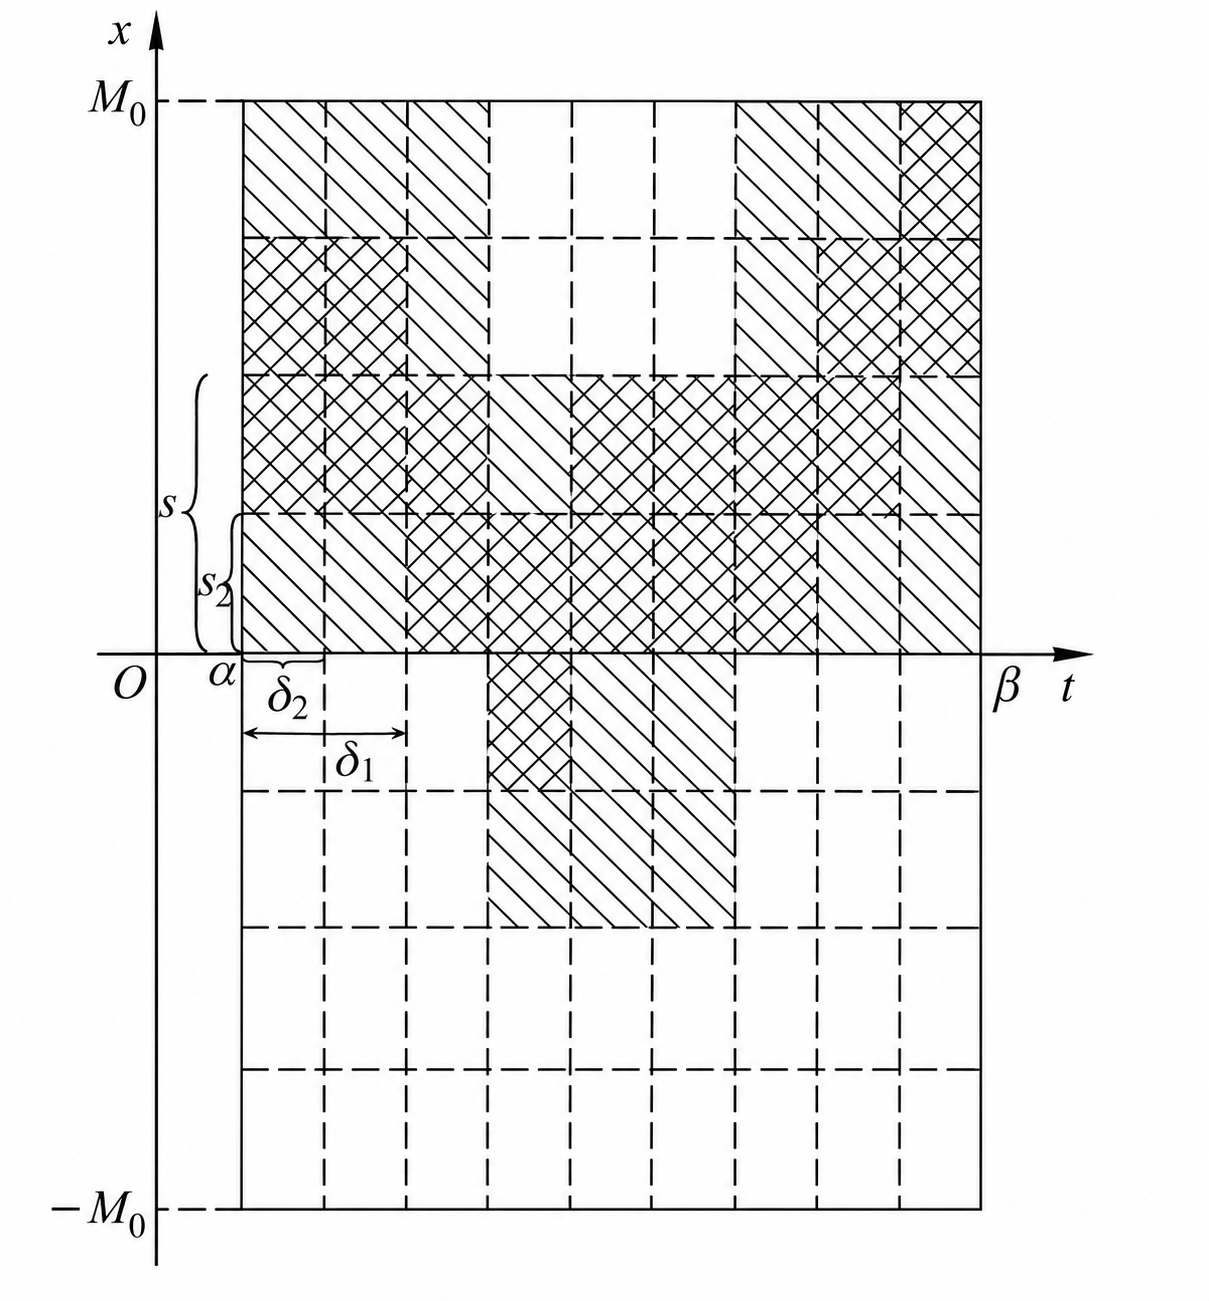
\includegraphics[width=0.5\linewidth]{figure/111}
\end{center}

	一般地，令
	\[
		s_k=\dfrac{M_0}{2^k}.
	\]
	可依次得到多边形 $S_k$ 及无穷函数族 $\mathcal{F}_k$，使得
	\[
		\mathcal{F}\supset\mathcal{F}_1
		\supset\cdots\supset\mathcal{F}_k\supset\cdots,
	\]
	并且对任意 $f_1^{(k)},f_2^{(k)}\in\mathcal{F}_k$，
	\[
		\abs{f_1^{(k)}(t)-f_2^{(k)}(t)}
		\leq2s_k
		=\dfrac{M_0}{2^{k-1}},
		\qquad t\in[\alpha,\beta].
	\]
	依次选取互不相同的 $f_k\in\mathcal{F}_k$。由于函数族逐层嵌套，
	对任意 $l\geq k$ 都有
	\[
		\abs{f_k(t)-f_l(t)}
		\leq\dfrac{M_0}{2^{k-1}},
		\qquad t\in[\alpha,\beta].
	\]
	故 $\{f_k\}$ 在 $[\alpha,\beta]$ 上一致满足 Cauchy 收敛准则，
	从而一致收敛。
\end{proof}

仍考虑初值问题
\[
	\dfrac{\dd x}{\dd t}=f(t,x),
	\qquad
	x(t_0)=x_0,
\]
但这里只要求 $f(t,x)$ 在矩形区域
\[
	R=\left\{
		(t,x)\in\R^2:
		\abs{t-t_0}\leq a,\ 
		\abs{x-x_0}\leq b
	\right\}
\]
上连续，不要求它关于 $x$ 满足 Lipschitz 条件。此时解仍然存在，
但不一定唯一。

\begin{theorem}(Peano 存在性定理)\label{thm:Peano存在性定理}
	若 $f(t,x)$ 在矩形区域 $R$ 上连续，则上述初值问题在区间
	\[
		I=[t_0-h,t_0+h]
	\]
	上至少有一个解，其中
	\[
		M=\max_{(t,x)\in R}\abs{f(t,x)},
		\qquad
		h=\min\left\{a,\dfrac{b}{M}\right\}.
	\]
	当 $M=0$ 时，约定取 $h=a$。
\end{theorem}

\begin{proof}
	\noindent\textbf{第一步：构造 Euler 折线。}\quad
	由
	\[
		\abs{x(t)-x_0}\leq M\abs{t-t_0}
	\]
	可知，为使所构造曲线的图像不越出 $R$，只需取
	$h=\min\{a,\dfrac{b}{M}\}$。

	任取正整数 $n$，令
	\[
		t_k=t_0+\dfrac{kh}{n},
		\qquad k=0,\pm1,\pm2,\ldots,\pm n,
	\]
	从而把区间 $I$ 分成 $2n$ 等份。从点
	$P_0=(t_0,x_0)$ 出发，以斜率 $f(t_0,x_0)$ 作直线段至
	$t=t_1$，记其端点为 $P_1=(t_1,x_1)$；再从 $P_1$ 出发，
	以斜率 $f(t_1,x_1)$ 作下一段。如此继续，得到
	\[
		x_{k+1}
		=x_k+f(t_k,x_k)(t_{k+1}-t_k),
		\qquad k=0,1,\ldots,n-1.
	\]
	向左作完全相同的构造，即得到整段 Euler 折线。

	\begin{figure}[htbp]
		\centering
		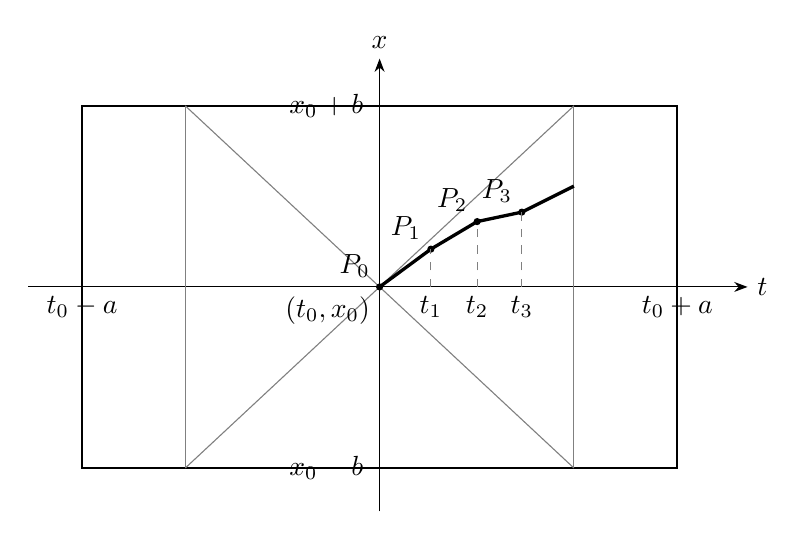
\begin{tikzpicture}[x=1.05cm,y=1cm,>=Stealth]
			\draw[->] (-4.25,0)--(4.45,0) node[right] {$t$};
			\draw[->] (0,-2.85)--(0,2.9) node[above] {$x$};
			\draw[thick] (-3.6,-2.3) rectangle (3.6,2.3);
			\draw[gray] (-2.35,-2.3)--(-2.35,2.3);
			\draw[gray] (2.35,-2.3)--(2.35,2.3);
			\draw[gray] (0,0)--(2.35,2.3);
			\draw[gray] (0,0)--(2.35,-2.3);
			\draw[gray] (0,0)--(-2.35,2.3);
			\draw[gray] (0,0)--(-2.35,-2.3);

			\draw[very thick]
				(0,0)
				--(0.62,0.48)
				--(1.18,0.83)
				--(1.72,0.95)
				--(2.35,1.28);
			\foreach \x/\y/\name in
				{0/0/P_0,0.62/0.48/P_1,1.18/0.83/P_2,1.72/0.95/P_3}
				{\fill (\x,\y) circle (1.3pt);
				 \node[above left] at (\x,\y) {$\name$};}
			\foreach \x/\y/\lab in
				{0.62/0.48/t_1,1.18/0.83/t_2,1.72/0.95/t_3}
				{\draw[dashed,gray] (\x,0)--(\x,\y);
				 \node[below] at (\x,0) {$\lab$};}

			\node[below left] at (0,0) {$(t_0,x_0)$};
			\node[left] at (-0.08,2.3) {$x_0+b$};
			\node[left] at (-0.08,-2.3) {$x_0-b$};
			\node[below] at (-3.6,0) {$t_0-a$};
			\node[below] at (3.6,0) {$t_0+a$};
		\end{tikzpicture}
		\caption{Euler 折线的构造}
		\label{fig:Euler折线构造}
	\end{figure}

	记所构造的折线函数为 $\varphi_n(t)$。对
	$s=0,1,\ldots,n-1$，它可写成
	\[
		\varphi_n(t)=
		\begin{cases}
			x_0+\displaystyle\sum_{k=0}^{s-1}
			f(t_k,x_k)(t_{k+1}-t_k)
			+f(t_s,x_s)(t-t_s),
			& t\in[t_s,t_{s+1}],\\[1.2em]
			x_0+\displaystyle\sum_{k=-s+1}^{0}
			f(t_k,x_k)(t_{k-1}-t_k)
			+f(t_{-s},x_{-s})(t-t_{-s}),
			& t\in(t_{-s-1},t_{-s}].
		\end{cases}
	\]
	当求和的下限大于上限时，约定该和为零。

	\noindent\textbf{第二步：证明 Euler 折线序列收敛。}\quad
	对任意 $n$，$\varphi_n$ 的图像始终位于 $R$ 内，故
	$\{\varphi_n\}$ 一致有界。每一段折线的斜率绝对值都不超过 $M$，
	因此对任意 $t,s\in I$，
	\[
		\abs{\varphi_n(t)-\varphi_n(s)}
		\leq M\abs{t-s}.
	\]
	所以 $\{\varphi_n\}$ 等度连续。由引理
	\ref{lem:AscoliArzela引理}，存在子序列
	$\{\varphi_{n_k}\}$ 在 $I$ 上一致收敛。记
	\[
		\varphi_{n_k}(t)\longrightarrow\varphi(t),
		\qquad t\in I.
	\]

	\noindent\textbf{第三步：证明 Euler 折线满足近似积分方程。}\quad
	只在 $[t_0,t_0+h]$ 上证明，左半区间完全相同。若
	$t\in[t_s,t_{s+1}]$，则对 $k=0,1,\ldots,s-1$，令
	\[
		d_n(k)
		=\int_{t_k}^{t_{k+1}}
		\left[
			f(t_k,x_k)-f\bigl(\tau,\varphi_n(\tau)\bigr)
		\right]\dd\tau,
	\]
	并令
	\[
		d_n^*(t)
		=\int_{t_s}^{t}
		\left[
			f(t_s,x_s)-f\bigl(\tau,\varphi_n(\tau)\bigr)
		\right]\dd\tau.
	\]
	于是利用积分的可加性可得
	\[
		\varphi_n(t)
		=x_0+\int_{t_0}^{t}
		f\bigl(\tau,\varphi_n(\tau)\bigr)\dd\tau
		+\sigma_n(t),
	\]
	其中
	\[
		\sigma_n(t)
		=\sum_{k=0}^{s-1}d_n(k)+d_n^*(t).
	\]

	下面证明 $\sigma_n\to0$。由于 $f$ 在紧集 $R$ 上一致连续，
	对任意 $\eps>0$，存在 $\delta>0$，使得当
	\[
		\abs{\tau-t_k}<\delta,
		\qquad
		\abs{\varphi_n(\tau)-x_k}<\delta
	\]
	时，有
	\[
		\abs{
			f(t_k,x_k)-f\bigl(\tau,\varphi_n(\tau)\bigr)
		}
		<\dfrac{\eps}{h}.
	\]
	当 $n$ 充分大时，
	\[
		\abs{t_{k+1}-t_k}
		=\dfrac{h}{n}<\delta,
	\]
	并且在每个小区间上
	\[
		\abs{\varphi_n(\tau)-x_k}
		\leq M\abs{\tau-t_k}
		\leq\dfrac{Mh}{n}<\delta.
	\]
	于是
	\[
		\abs{d_n(k)}<\dfrac{\eps}{n},
		\qquad
		\abs{d_n^*(t)}<\dfrac{\eps}{n}.
	\]
	因为 $s\leq n-1$，所以
	\[
		\abs{\sigma_n(t)}
		<\dfrac{s}{n}\eps+\dfrac{\eps}{n}
		\leq\eps.
	\]
	故 $\sigma_n(t)\to0$，而且收敛关于 $t$ 是一致的。

	\noindent\textbf{第四步：取极限。}\quad
	由 $\varphi_{n_k}\to\varphi$ 的一致收敛以及 $f$ 在 $R$ 上的一致连续性，
	\[
		f\bigl(t,\varphi_{n_k}(t)\bigr)
		\longrightarrow
		f\bigl(t,\varphi(t)\bigr)
	\]
	也一致成立。在近似积分方程中令 $k\to\infty$，得到
	\[
		\varphi(t)
		=x_0+\int_{t_0}^{t}
		f\bigl(\tau,\varphi(\tau)\bigr)\dd\tau,
		\qquad t\in I.
	\]
	因此 $\varphi$ 满足原初值问题的等价积分方程，从而是原初值问题的解。
\end{proof}

从几何上看，Euler 折线法给出了一种用折线逼近积分曲线的方法。

\begin{definition}\label{def:epsilon逼近解}
	定义在区间 $[\alpha,\beta]$ 上的函数 $x=\varphi(t)$
	称为上述初值问题在该区间上的一个 \textbf{$\eps$-逼近解}，如果
	$\varphi(t_0)=x_0$，并且满足：
	\begin{enumerate}
		\item $\varphi$ 在 $[\alpha,\beta]$ 上连续，除有限多个点外处处
			连续可微，并且在这些分点处的左、右导数都存在；
		\item 对任意 $t\in[\alpha,\beta]$，点
			$(t,\varphi(t))$ 都位于矩形区域 $R$ 内；
		\item 对任意 $t\in[\alpha,\beta]$，
			\[
				\abs{
					\dfrac{\dd\varphi(t)}{\dd t}
					-f\bigl(t,\varphi(t)\bigr)
				}\leq\eps.
			\]
	\end{enumerate}
	在不可微的分点处，若 $t\neq\beta$，上式中的导数取右导数；
	当 $t=\beta$ 时取左导数。
\end{definition}

\begin{proposition}\label{prop:Peano条件下epsilon逼近解的存在性}
	若 $f(t,x)$ 在矩形区域 $R$ 上连续，则对任意 $\eps>0$，
	初值问题在区间 $I=[t_0-h,t_0+h]$ 上存在 $\eps$-逼近解。
	由 Euler 折线得到的逼近解在右半区间上还满足
	\[
		\abs{\varphi(t)-\varphi(s)}
		\leq M\abs{t-s},
		\qquad t,s\in[t_0,t_0+h],
	\]
	其中
	\[
		h=\min\left\{a,\dfrac{b}{M}\right\},
		\qquad
		M=\max_{(t,x)\in R}\abs{f(t,x)}.
	\]
\end{proposition}

\subsection*{唯一性条件下的Euler折线}
Peano 定理利用紧性从 Euler 折线中抽取收敛子列。若另有 Lipschitz 条件，则第~\ref{sec:picard-contraction}~节的残差估计还能控制整个近似序列。
必要时缩小共同存在区间，仍记其半长为 $h$，并使 $Lh<1$。在该区间的连续函数闭集上，令
\[
 (Au)(t)=x_0+\int_{t_0}^tf(s,u(s))\,ds.
\]
记初值问题的解为 $x$，则 $Ax=x$，且对任一留在该闭集内的近似曲线 $u$，
\[
 \|u-x\|_\infty\leq\|u-Au\|_\infty/(1-Lh).
\]
在 Peano 定理的证明中已经得到 Euler 折线 $u_n$ 满足
\[
 u_n=Au_n+\sigma_n,\qquad\|\sigma_n\|_\infty\longrightarrow0.
\]
代入残差估计，便有
\[
 \|u_n-x\|_\infty\leq\frac{\|\sigma_n\|_\infty}{1-Lh}\longrightarrow0.
\]
因此在这个共同小区间上，整个 Euler 折线序列均一致收敛到解，而不只是某个子序列。

\section{解的延拓}\label{sec:解的延拓}

前面所得的存在性定理只保证初值问题在初始点附近有解。现在讨论：
已经得到的局部解能否继续向两端延伸，以及它最终能延伸到什么地方。

设 $f(t,x)$ 在开区域 $G\subset\R^2$ 内连续，$x=\varphi(t)$
是方程
\[
	\dfrac{\dd x}{\dd t}=f(t,x)
\]
在闭区间 $[\alpha,\beta]$ 上的一个解，并且其图像位于 $G$ 内。
由于
\[
	Q=\bigl(\beta,\varphi(\beta)\bigr)\in G,
\]
可在 $Q$ 的附近取一个完全落在 $G$ 内的小矩形。由定理
\ref{thm:Peano存在性定理}，
存在 $h_1>0$，使初值问题
\[
	\dfrac{\dd x}{\dd t}=f(t,x),
	\qquad x(\beta)=\varphi(\beta)
\]
在 $[\beta-h_1,\beta+h_1]$ 上有解 $x=\varphi_1(t)$。
同理，在左端点处存在 $h_2>0$ 以及定义在
$[\alpha-h_2,\alpha+h_2]$ 上的解 $x=\varphi_2(t)$，满足
$\varphi_2(\alpha)=\varphi(\alpha)$。于是分段函数
\[
	\psi(t)=
	\begin{cases}
		\varphi_2(t), & t\in[\alpha-h_2,\alpha],\\
		\varphi(t),   & t\in[\alpha,\beta],\\
		\varphi_1(t), & t\in[\beta,\beta+h_1]
	\end{cases}
\]
仍是原方程的解，并把 $\varphi$ 延伸到了更大的区间
$[\alpha-h_2,\beta+h_1]$ 上。几何上，这相当于在原积分曲线的两个端点
继续接上新的积分曲线段。

\begin{figure}[htbp]
	\centering
	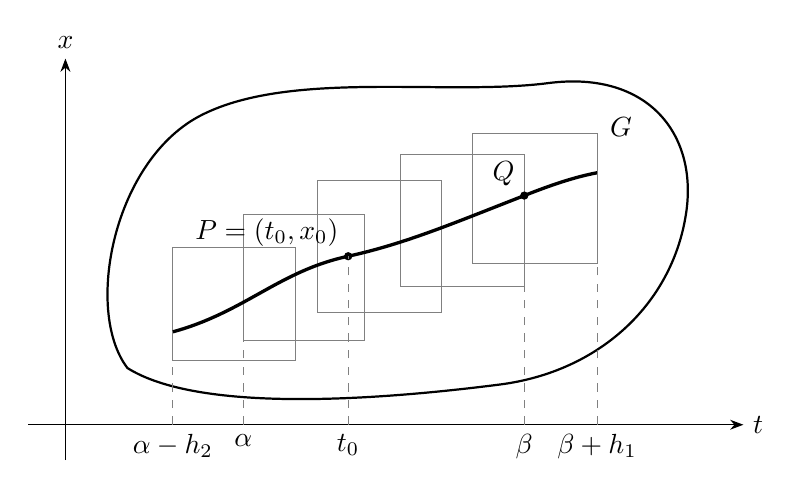
\begin{tikzpicture}[x=1.05cm,y=1cm,>=Stealth]
		\draw[->] (-0.45,0)--(8.2,0) node[right] {$t$};
		\draw[->] (0,-0.45)--(0,4.65) node[above] {$x$};

		\draw[thick]
			(0.75,0.72)
			.. controls (0.22,1.45) and (0.58,3.38) .. (1.66,3.94)
			.. controls (2.75,4.51) and (4.62,4.17) .. (5.85,4.34)
			.. controls (7.06,4.50) and (7.67,3.67) .. (7.50,2.64)
			.. controls (7.32,1.52) and (6.45,0.67) .. (5.25,0.51)
			.. controls (3.68,0.30) and (1.60,0.16) .. cycle;
		\node at (6.72,3.78) {$G$};

		\draw[gray] (1.30,0.82) rectangle (2.78,2.25);
		\draw[gray] (2.15,1.07) rectangle (3.62,2.67);
		\draw[gray] (3.05,1.43) rectangle (4.55,3.10);
		\draw[gray] (4.05,1.75) rectangle (5.55,3.43);
		\draw[gray] (4.92,2.05) rectangle (6.43,3.70);

		\draw[very thick]
			(1.30,1.18)
			.. controls (2.17,1.43) and (2.58,1.95) .. (3.42,2.14)
			.. controls (4.12,2.30) and (4.74,2.58) .. (5.55,2.91)
			.. controls (5.91,3.06) and (6.18,3.15) .. (6.43,3.20);

		\fill (3.42,2.14) circle (1.5pt)
			node[above left] {$P=(t_0,x_0)$};
		\fill (5.55,2.91) circle (1.5pt)
			node[above left] {$Q$};

		\foreach \u/\v/\lab in
			{1.30/1.18/{\alpha-h_2},2.15/1.42/{\alpha},3.42/2.14/{t_0},5.55/2.91/{\beta},6.43/3.20/{\beta+h_1}}
			{
				\draw[dashed,gray] (\u,0)--(\u,\v);
				\node[below] at (\u,0) {$\lab$};
			}
	\end{tikzpicture}
	\caption{解的延拓}
	\label{fig:解的延拓}
\end{figure}

\begin{definition}\label{def:解的延拓与饱和解}
	设 $x=\varphi(t)$ 与 $x=\psi(t)$ 分别是定义在区间 $J_1,J_2$
	上的解。若 $J_1\subset J_2$，且 $\psi(t)=\varphi(t)$ 对所有
	$t\in J_1$ 成立，则称 $\psi$ 是 $\varphi$ 在 $J_2$ 上的
	\textbf{延拓}。若一个解不能再延拓到任何更大的区间，则称它为
	\textbf{饱和解}或\textbf{极大解}。
\end{definition}

\begin{theorem}[有限端点延拓判据]\label{thm:有限端点延拓判据}
	设 $f(t,x)$ 在区域 $G$ 内有界，并且关于 $x$ 局部满足
	Lipschitz 条件。若初值问题的饱和解 $x=\varphi(t)$ 的最大存在
	区间为
	\[
		-\infty<\alpha<t<\beta<+\infty,
	\]
	则极限
	\[
		\varphi(\alpha+0)
		=\lim_{t\to\alpha^+}\varphi(t),
		\qquad
		\varphi(\beta-0)
		=\lim_{t\to\beta^-}\varphi(t)
	\]
	都存在，且
	\[
		\bigl(\alpha,\varphi(\alpha+0)\bigr),
		\qquad
		\bigl(\beta,\varphi(\beta-0)\bigr)
	\]
	均为 $G$ 的边界点。
\end{theorem}

\begin{proof}
	设 $\abs{f(t,x)}\leq M$。当
	$\alpha<t_2<t_1<\beta$ 时，由积分方程，
	\[
		\begin{aligned}
		\abs{\varphi(t_1)-\varphi(t_2)}
		&=\abs{\int_{t_2}^{t_1}
		f\bigl(t,\varphi(t)\bigr)\dd t}\\
		&\leq M\abs{t_1-t_2}.
		\end{aligned}
	\]
	因此当 $t_1,t_2\to\alpha^+$ 时，
	$\varphi(t_1)-\varphi(t_2)\to0$。由 Cauchy 收敛准则，
	$\varphi(\alpha+0)$ 存在；同理，
	$\varphi(\beta-0)$ 存在。

	若 $\bigl(\alpha,\varphi(\alpha+0)\bigr)$ 是 $G$ 的内点，则可由
	Picard 存在唯一性定理将解延拓到某个区间
	\[
		\alpha-h_*<t<\beta,
		\qquad h_*>0,
	\]
	这与 $(\alpha,\beta)$ 为最大存在区间矛盾。故
	$\bigl(\alpha,\varphi(\alpha+0)\bigr)$ 为 $G$ 的边界点；右端点的
	结论同理。
\end{proof}

沿选定的解分支不断重复上述过程，可以得到饱和解；严格地说，也可由极大原理
保证其存在。饱和解的存在区间必为开区间。事实上，若右端点 $b$ 有限且
属于其存在区间，则 $(b,\varphi(b))\in G$，由定理
\ref{thm:Peano存在性定理} 还可越过
$b$ 继续延拓，这与饱和性矛盾；左端点同理。

为刻画积分曲线与边界的接近程度，定义点 $(t_0,x_0)$ 到集合
$D\subset\R^2$ 的距离为
\[
	\rho\bigl((t_0,x_0),D\bigr)
	=\inf_{(t,x)\in D}
	\sqrt{(t-t_0)^2+(x-x_0)^2}.
\]

定理 \ref{thm:有限端点延拓判据} 的两个附加条件---$f$ 在整个
$G$ 内有界，以及最大存在区间的端点有限---在下面的结论中都不再要求。
相应地，下面只能断言积分曲线延拓到区域的边界；若该边界位于无穷远处，
并不意味着 $\varphi(t)$ 在某个有限端点有极限。

\begin{theorem}[解的延拓定理]\label{thm:解的延拓定理}
	设 $G$ 为 $\R^2$ 上的一个开区域，$f(t,x)$ 在 $G$ 内连续。
	并且关于 $x$ 局部满足 Lipschitz 条件。
	对于方程的任一饱和解 $x=\varphi(t)$，积分曲线
	$x=\varphi(t)$ 必能达到 $G$ 的边界。特别地，当 $G$ 为有界区域，
	且饱和解 $x=\varphi(t)$ 的存在区间为 $(a,b)$ 时，
	\[
		\lim_{t\to b^-}
		\rho\bigl((t,\varphi(t)),\partial G\bigr)=0,
		\qquad
		\lim_{t\to a^+}
		\rho\bigl((t,\varphi(t)),\partial G\bigr)=0.
	\]
\end{theorem}

\begin{proof}
	把饱和解 $\varphi(t)$ 的最大存在区间记为 $J$。只证明
	$t\to b^-$ 时的结论；$t\to a^+$ 时完全类似。令
	\[
		J_+=J\cap[t_0,+\infty).
	\]

	\noindent\textbf{情形 1}
	若 $J_+=[t_0,+\infty)$，即 $b=+\infty$，则积分曲线在 $G$ 内
	可以延拓到无穷，因而在无穷远处达到 $\partial G$。

	\noindent\textbf{情形 2}
	若 $J_+=[t_0,b)$ 且 $b<+\infty$，则只需证明
	\[
		\lim_{t\to b^-}\bigl(t,\varphi(t)\bigr)\in\partial G.
	\]
	换言之，积分曲线不能始终停留在 $G$ 内的某个有界闭区域中。
	也就是说，对于任意有界闭区域
	$G_1\subset G$，不可能有
	\[
		\bigl(t,\varphi(t)\bigr)\in G_1,
		\qquad \forall t\in J_+.
	\]
	反设存在这样的 $G_1$。由于 $G_1$ 为有界闭集，且 $f$ 在
	$G_1$ 上连续，故存在常数 $K>0$，使得
	\[
		\abs{f(t,x)}\leq K,
		\qquad \forall (t,x)\in G_1.
	\]
	于是
	\[
		\abs{\varphi'(t)}
		=\abs{f\bigl(t,\varphi(t)\bigr)}
		\leq K,
		\qquad \forall t\in J_+.
	\]
	由微分中值定理，对于任意 $t_1,t_2\in J_+$，都有
	\[
		\abs{\varphi(t_2)-\varphi(t_1)}
		\leq K\abs{t_2-t_1}.
	\]
	因此，当 $t\to b^-$ 时，$\varphi(t)$ 满足 Cauchy 收敛准则，
	故极限存在。设
	\[
		\lim_{t\to b^-}\varphi(t)=x_*.
	\]
	由于 $G_1$ 为闭集，所以 $(b,x_*)\in G_1\subset G$。定义
	\[
		\varphi_*(t)=
		\begin{cases}
			\varphi(t), & t\in[t_0,b),\\
			x_*, & t=b.
		\end{cases}
	\]
	显然 $\varphi_*(t)$ 在 $[t_0,b]$ 上连续。对 $\varphi(t)$ 满足的
	等价积分方程在 $t\to b^-$ 时取极限，得到
	\[
		\varphi_*(t)
		=x_0+\int_{t_0}^{t}
		f\bigl(s,\varphi_*(s)\bigr)\dd s,
		\qquad t\in[t_0,b].
	\]
	故 $\varphi_*(t)$ 是原初值问题在 $[t_0,b]$ 上的解。再由定理
	\ref{thm:Peano存在性定理}，它还可从点 $(b,x_*)$ 向右延拓，
	这与 $J_+=[t_0,b)$ 是最大存在区间矛盾。

	因此积分曲线不可能停留在 $G$ 内的任何有界闭区域中，只能向
	$G$ 的边界任意接近。当 $G$ 有界时，这正说明
	\[
		\rho\bigl((t,\varphi(t)),\partial G\bigr)\to0,
		\qquad t\to b^-.
	\]
	左端的结论同理可得。
\end{proof}

\begin{proposition}[有限维紧集延拓判据]\label{prop:compact-extension-vector}
设 $G\subset\R\times\R^n$ 为开集，$f:G\to\R^n$ 连续，且关于 $x$ 局部满足 Lipschitz 条件。
若解 $x(t)$ 定义在 $[t_0,\beta)$，$\beta<\infty$，并且其图像始终包含在某个紧集 $K\subset G$ 中，
则该解能够越过 $\beta$ 延拓。左端点有相同结论。
\end{proposition}
\begin{proof}
这正是前面延拓证明的有限维形式。连续性与紧性给出 $\sup_K|f|=M<\infty$，故
\[
 |x(t)-x(s)|\leq M|t-s|,\qquad t_0\leq s,t<\beta.
\]
因此 $t\uparrow\beta$ 时 $x(t)$ 满足 Cauchy 准则，在 $\R^n$ 中有极限 $x_*$。
$K$ 为闭集，故 $(\beta,x_*)\in K\subset G$。
令 $x(\beta)=x_*$，在积分方程中取极限，知延长的函数仍满足积分方程。
再在 $(\beta,x_*)$ 应用有限维 Picard 定理，便可将解继续接到 $\beta$ 右侧。
由唯一性两段解相容。反向时间给出左端结论。
\end{proof}

由定理可知，当 $G$ 无界时，一个解向右延拓只有两种可能：或者存在于
$[t_0,+\infty)$；或者只存在于 $[t_0,m)$，其中 $m<+\infty$，并且当
$t\to m^-$ 时，$\varphi(t)$ 无界，或点
$(t,\varphi(t))$ 趋近于 $G$ 的边界。

现在考虑无界带形区域
\[
	G=\bigl\{(t,x)\in\R^2:T_0<t<T_1,\ -\infty<x<+\infty\bigr\}.
\]

\begin{corollary}\label{cor:有界饱和解的全区间存在性}
	若 $f(t,x)$ 在上述带形区域 $G$ 内连续，并且饱和解
	$x=\varphi(t)$ 有界，则它的存在区间必为 $(T_0,T_1)$。
\end{corollary}

\begin{proof}
	设 $\varphi$ 的存在区间为 $(a,b)$。若 $b<T_1$，取
	$t_0\in(a,b)$，并设 $\abs{\varphi(t)}\leq M$。当 $t\in[t_0,b)$ 时，
	积分曲线位于紧集
	\[
		[t_0,b]\times[-M,M]\subset G
	\]
	内，这与定理 \ref{thm:解的延拓定理} 矛盾。因此 $b=T_1$；
	同理可得 $a=T_0$。
\end{proof}

\begin{corollary}[全空间中有界解的全局存在性]
	\label{cor:全空间中有界解的全局存在性}
	设 $f(t,x)$ 在 $\R^2$ 内连续，并且关于 $x$ 局部满足 Lipschitz
	条件。若初值问题的解 $x=\varphi(t)$ 有界，则它的最大存在区间为
	\[
		(-\infty,+\infty).
	\]
\end{corollary}

\begin{proof}
	由定理 \ref{thm:解的延拓定理}，解的积分曲线只能趋近
	$\R^2$ 的边界。又因 $\varphi(t)$ 有界，故只能有
	$\abs{t}\to+\infty$，从而其最大存在区间为
	$(-\infty,+\infty)$。
\end{proof}

\begin{theorem}[自治系统的有界内陷区域]\label{thm:自治系统的有界内陷区域}
	考虑自治系统
	\[
		\dfrac{\dd\vect{x}}{\dd t}=\vect{f}(\vect{x}),
		\qquad
		\vect{x}(t_0)=\vect{x}_0.
	\]
	设 $\vect{f}$ 在区域 $D\subset\R^n$ 上连续，并且关于
	$\vect{x}$ 局部满足 Lipschitz 条件。若解的轨道
	$\vect{x}=\vect{\varphi}(t,\vect{x}_0)$ 始终停留在有界区域
	\[
		\Gamma\subset D\subset\R^n,
		\qquad
		\rho(\Gamma,\partial D)>0,
	\]
	则该解可延拓到 $(-\infty,+\infty)$。
\end{theorem}

\begin{proof}
	把自治系统看成 $(t,\vect{x})$ 空间中的方程组，并取定义区域
	\[
		G=D\times(-\infty,+\infty).
	\]
	由定理 \ref{thm:解的延拓定理}，若解不能延拓到整个实轴，则其
	积分曲线必须趋近 $G$ 的边界。可是轨道始终在 $\Gamma$ 内，
	并且 $\rho(\Gamma,\partial D)>0$；时间变量也可在
	$(-\infty,+\infty)$ 中任意延伸，故积分曲线不可能趋近
	$\partial G$。矛盾。
\end{proof}

\begin{theorem}[线性增长条件下的全局存在性]
	\label{cor:线性增长条件下的全区间存在性}
	设 $f(t,x)$ 在 $\R^2$ 内连续，并且关于 $x$ 局部满足 Lipschitz
	条件。若存在常数 $N>0$，使得
	\[
		\abs{f(t,x)}\leq N\abs{x},
		\qquad (t,x)\in\R^2,
	\]
	则初值问题的任一解都存在于 $(-\infty,+\infty)$ 上。
\end{theorem}

\begin{proof}
	设饱和解 $x=\varphi(t)$ 的存在区间为 $(a,b)$。只需证明
	$b=+\infty$。反设 $b<+\infty$，固定 $t_0\in(a,b)$。若 $\varphi$ 在
	$(t_0,b)$ 上无界，则对任意充分大的 $K$，可取
	$t_K\in(t_0,b)$，使 $\abs{\varphi(t_K)}=K$，并取 $t_K$ 之前
	最后一次达到 $\abs{\varphi(t_0)}+1$ 的时刻 $\tau_K$。在
	$[\tau_K,t_K]$ 上 $\abs{\varphi(t)}>0$，且
	\[
		\dfrac{\dd}{\dd t}\abs{\varphi(t)}
		\leq\abs{f\bigl(t,\varphi(t)\bigr)}
		\leq N\abs{\varphi(t)}.
	\]
	积分得到
	\[
		\ln\dfrac{\abs{\varphi(t_K)}}{\abs{\varphi(\tau_K)}}
		\leq N(t_K-\tau_K)
		\leq N(b-t_0),
	\]
	从而
	\[
		K\leq
		\bigl(\abs{\varphi(t_0)}+1\bigr)\mathrm{e}^{N(b-t_0)}.
	\]
	这与 $K$ 可任意大矛盾。因此 $\varphi$ 在 $(t_0,b)$ 上有界，
	由推论 \ref{cor:全空间中有界解的全局存在性} 可知它可以延拓到
	$+\infty$，仍与 $b<+\infty$ 矛盾。
	故 $b=+\infty$；左端同理。
\end{proof}

\begin{corollary}[有界向量场下的延拓]
	\label{cor:有界向量场下的延拓}
	考虑自治系统
	\[
		\dfrac{\dd\vect{x}}{\dd t}=\vect{f}(\vect{x}),
		\qquad
		\vect{x}(t_0)=\vect{x}_0.
	\]
	设 $\vect{f}$ 在区域 $D\subset\R^n$ 上连续有界，并且关于
	$\vect{x}$ 局部满足 Lipschitz 条件。若一条饱和解的轨道在其两个
	时间端点附近都具有无限的几何长度，则该解存在于
	$(-\infty,+\infty)$ 上。
\end{corollary}

\begin{proof}
	设 $\norm{\vect{f}(\vect{x})}\leq M$。若右端点 $b$ 有限，则
	轨道从 $t_0$ 到 $b$ 的弧长至多为
	\[
		\int_{t_0}^{b}
		\norm{\vect{f}\bigl(\vect{x}(t)\bigr)}\dd t
		\leq M(b-t_0),
	\]
	与右端附近弧长无限矛盾。因此 $b=+\infty$；左端同理。
\end{proof}

\begin{corollary}[全空间中有界向量场的全局存在性]
	\label{cor:全空间中有界向量场的全局存在性}
	若 $\vect{f}:\R^n\to\R^n$ 连续有界，并且关于 $\vect{x}$ 局部
	满足 Lipschitz 条件，则自治初值问题
	\[
		\dfrac{\dd\vect{x}}{\dd t}=\vect{f}(\vect{x}),
		\qquad
		\vect{x}(t_0)=\vect{x}_0
	\]
	的解存在于 $(-\infty,+\infty)$ 上。
\end{corollary}

\begin{proof}
	设 $\norm{\vect{f}(\vect{x})}\leq M$。若解的右端点 $b$ 有限，
	则当 $t_0\leq t<b$ 时，
	\[
		\norm{\vect{x}(t)}
		\leq\norm{\vect{x}_0}+M\abs{t-t_0}
		\leq\norm{\vect{x}_0}+M(b-t_0).
	\]
	故该解在右端点附近有界。由推论
	\ref{cor:全空间中有界解的全局存在性}，它可延拓到
	$+\infty$，矛盾。左端同理。
\end{proof}

上述结论可推广到有限维方程组。

\begin{theorem}[Wintner 定理]\label{cor:Wintner延拓定理}
	设向量函数 $\vect{f}(t,\vect{x})$ 在
	$(t,\vect{x})$ 全空间内连续，并且关于 $\vect{x}$ 局部满足
	Lipschitz 条件。又设
	\[
		\norm{\vect{f}(t,\vect{x})}\leq L(r),
		\qquad
		r=\norm{\vect{x}}
		=\left(\sum_{i=1}^{n}x_i^2\right)^{\!1/2},
	\]
	其中 $L(r)$ 在 $r\geq0$ 上连续，在 $r>0$ 时为正，且对任意
	$\alpha>0$ 都有
	\[
		\int_{\alpha}^{+\infty}\dfrac{\dd r}{L(r)}=+\infty.
	\]
	则初值问题
	\[
		\dfrac{\dd\vect{x}}{\dd t}=\vect{f}(t,\vect{x}),
		\qquad
		\vect{x}(t_0)=\vect{x}_0
	\]
	的解存在于 $(-\infty,+\infty)$ 上。
\end{theorem}

\begin{proof}
	设饱和解 $\vect{x}=\vect{x}(t)$ 的存在区间为 $(a,b)$，并令
	$r(t)=\norm{\vect{x}(t)}$。只证 $b=+\infty$。反设 $b<+\infty$ 且
	$r(t)$ 在 $(t_0,b)$ 上无界。对任意充分大的 $K$，取
	$t_K\in(t_0,b)$ 与 $\tau_K<t_K$，使
	\[
		r(t_K)=K,
		\qquad
		r(\tau_K)=r(t_0)+1,
		\qquad
		r(t)>0\quad(t\in[\tau_K,t_K]).
	\]
	在此区间上，由 Cauchy--Schwarz 不等式，
	\[
		\dfrac{\dd r}{\dd t}
		=\dfrac{\left\langle\vect{x},\vect{x}'\right\rangle}
		{\norm{\vect{x}}}
		\leq\norm{\vect{x}'}
		\leq L(r).
	\]
	因此
	\[
		\int_{r(t_0)+1}^{K}\dfrac{\dd r}{L(r)}
		\leq t_K-\tau_K
		\leq b-t_0.
	\]
	令 $K\to+\infty$，便与积分发散条件矛盾。所以 $r(t)$ 在
	$(t_0,b)$ 上有界。此时向量版的延拓定理表明该解可越过 $b$
	继续延拓，故 $b=+\infty$。左端同理。
\end{proof}

\subsection*{利用能量证明解的全局存在性}
第二章中保守系统的能量守恒也可用于讨论解的延拓。若势能有下界，则由能量守恒可得速度有界；在有限时间区间内积分，又可得位置有界。
\begin{theorem}[能量与全局延拓]\label{thm:energy-global-extension}
设 $U\in C^2(\R^n)$ 有下界，$m_i>0$。则
$m_i\ddot x_i=-\partial_iU(x)$ 的每个解都能双向延拓到整条时间轴。
\end{theorem}
\begin{proof}
把二阶方程写成状态变量 $(x,v)$ 的一阶方程
$\dot x_i=v_i,\ \dot v_i=-\partial_iU(x)/m_i$。其向量场为 $C^1$，
所以每个初值有唯一最大解。沿该解计算
\[
 \frac{d}{dt}\left(\frac12\sum_i m_iv_i^2+U(x)\right)
 =\sum_i v_i\bigl(m_i\dot v_i+\partial_iU(x)\bigr)=0.
\]
设常能量为 $E_0$，取 $C$ 使 $U(x)\geq-C$，再令 $m_*:=\min_i m_i>0$。
于是
\[
 \begin{aligned}
 \frac{m_*}{2}|v(t)|^2&\leq\frac12\sum_i m_iv_i(t)^2\\
 &=E_0-U(x(t))\\
 &\leq E_0+C.
\end{aligned}
\]
因此存在与时间无关的 $M$，使 $|v(t)|\leq M$。
若最大正向存在端点 $\beta$ 有限，则对 $t_0\leq t<\beta$，
\[
 |x(t)|\leq |x(t_0)|+\int_{t_0}^t|v(s)|\,ds
 \leq |x(t_0)|+M(\beta-t_0).
\]
所以 $(x(t),v(t))$ 始终留在整个状态空间中的一个紧球内。
命题~\ref{prop:compact-extension-vector} 说明解可越过 $\beta$ 延拓，与最大性矛盾。
负向时间同样有
$|x(t)|\leq|x(t_0)|+M|t-t_0|$，故负向端点也不可能有限。
两个方向的最大端点分别为 $+\infty$ 和 $-\infty$。
\end{proof}

\section{微分不等式与比较定理}\label{sec:微分不等式与比较定理}

\begin{theorem}(Gronwall 不等式)\label{thm:Gronwall不等式}
	设 $x(t),f(t)$ 为区间 $[t_0,t_1]$ 上的实连续函数，$f(t)\geq0$。
	若存在实常数 $g$，使得
	\[
		x(t)\leq g+\int_{t_0}^{t}f(\tau)x(\tau)\dd\tau,
		\qquad t\in[t_0,t_1],
	\]
	则
	\[
		x(t)\leq g\exp\left(\int_{t_0}^{t}f(\tau)\dd\tau\right),
		\qquad t\in[t_0,t_1].
	\]
\end{theorem}

\begin{proof}
	令
	\[
		y(t)=g+\int_{t_0}^{t}f(\tau)x(\tau)\dd\tau.
	\]
	则 $x(t)\leq y(t)$，并且
	\[
		y'(t)=f(t)x(t)\leq f(t)y(t).
	\]
	因此
	\[
		\dfrac{\dd}{\dd t}
		\left\{
		\exp\left(-\int_{t_0}^{t}f(\tau)\dd\tau\right)y(t)
		\right\}\leq0.
	\]
	从 $t_0$ 到 $t$ 积分，得到
	\[
		\exp\left(-\int_{t_0}^{t}f(\tau)\dd\tau\right)y(t)
		\leq y(t_0)=g.
	\]
	故
	\[
		x(t)\leq y(t)
		\leq g\exp\left(\int_{t_0}^{t}f(\tau)\dd\tau\right).
	\]
\end{proof}

\begin{theorem}(推广的 Gronwall 不等式)\label{thm:推广的Gronwall不等式}
	设 $x(t),g(t)$ 为区间 $[t_0,t_1]$ 上的实连续函数，函数
	$f(t)\geq0$ 在区间 $[t_0,t_1]$ 上可积。若它们满足
	\[
		x(t)\leq g(t)+\int_{t_0}^{t}f(\tau)x(\tau)\dd\tau,
		\qquad t\in[t_0,t_1],
	\]
	则当 $t\in[t_0,t_1]$ 时，
	\[
		x(t)\leq g(t)
		+\int_{t_0}^{t}f(\tau)g(\tau)
		\exp\left(\int_{\tau}^{t}f(s)\dd s\right)\dd\tau.
	\]
\end{theorem}

\begin{proof}
	先设 $f(t)$ 连续。在已知不等式两边分别乘以 $f(t)$，得到
	\[
		f(t)x(t)\leq f(t)g(t)
		+f(t)\int_{t_0}^{t}f(\tau)x(\tau)\dd\tau.
	\]
	令
	\[
		H(t)=\int_{t_0}^{t}f(\tau)x(\tau)\dd\tau,
	\]
	则上式可写成
	\[
		\dfrac{\dd H(t)}{\dd t}-f(t)H(t)\leq f(t)g(t).
	\]
	两边分别乘以
	\[
		\exp\left(-\int_{t_0}^{t}f(\tau)\dd\tau\right),
	\]
	得到
	\[
		\dfrac{\dd}{\dd t}
		\left\{
		H(t)\exp\left(-\int_{t_0}^{t}f(\tau)\dd\tau\right)
		\right\}
		\leq f(t)g(t)
		\exp\left(-\int_{t_0}^{t}f(\tau)\dd\tau\right).
	\]
	在上式两边从 $t_0$ 到 $t$ 积分，得
	\[
		H(t)\exp\left(-\int_{t_0}^{t}f(\tau)\dd\tau\right)
		\leq
		\int_{t_0}^{t}f(\tau)g(\tau)
		\exp\left(\int_{\tau}^{t_0}f(s)\dd s\right)\dd\tau.
	\]
	即
	\[
		H(t)\leq
		\int_{t_0}^{t}f(\tau)g(\tau)
		\exp\left(\int_{\tau}^{t}f(s)\dd s\right)\dd\tau.
	\]
	再由原不等式得到
	\[
		x(t)\leq g(t)+H(t)
		\leq g(t)
		+\int_{t_0}^{t}f(\tau)g(\tau)
		\exp\left(\int_{\tau}^{t}f(s)\dd s\right)\dd\tau.
	\]

	当 $f$ 仅为可积函数时，对原不等式右端逐次代入。对任意
	$n=0,1,2,\ldots$，可得
	\[
	\begin{aligned}
		x(t)\leq{}&g(t)
		+\int_{t_0}^{t}f(\tau)g(\tau)
		\sum_{k=0}^{n}\dfrac{1}{k!}
		\left(\int_{\tau}^{t}f(s)\dd s\right)^k\dd\tau
		+R_n(t),
	\end{aligned}
	\]
	其中
	\[
		R_n(t)=\int_{t_0}^{t}f(\tau)x(\tau)
		\dfrac{1}{(n+1)!}
		\left(\int_{\tau}^{t}f(s)\dd s\right)^{n+1}\dd\tau.
	\]
	由于 $x$ 在闭区间上有界，且 $f$ 可积，所以 $R_n(t)\to0$；
	同时上式中的级数绝对收敛。令 $n\to\infty$，便得到同一结论。
\end{proof}

\begin{corollary}\label{cor:Gronwall单调函数推论}
	在定理 \ref{thm:推广的Gronwall不等式} 的条件下，如果附加条件
	$g(t)$ 连续且导数 $g'(t)\geq0$，则
	\[
		x(t)\leq g(t)
		\exp\left(\int_{t_0}^{t}f(\tau)\dd\tau\right),
		\qquad t\in[t_0,t_1].
	\]
\end{corollary}

\begin{proof}
	对定理 \ref{thm:推广的Gronwall不等式} 的结论作分部积分，得到
	\[
	\begin{aligned}
		x(t)\leq{}&g(t_0)
		\exp\left(\int_{t_0}^{t}f(\tau)\dd\tau\right)\\
		&+\int_{t_0}^{t}g'(\tau)
		\exp\left(\int_{\tau}^{t}f(s)\dd s\right)\dd\tau\\
		\leq{}&\exp\left(\int_{t_0}^{t}f(\tau)\dd\tau\right)
		\left\{g(t_0)+\int_{t_0}^{t}g'(\tau)\dd\tau\right\}\\
		={}&g(t)\exp\left(\int_{t_0}^{t}f(\tau)\dd\tau\right).
	\end{aligned}
	\]
\end{proof}

利用推论 \ref{cor:Gronwall单调函数推论} 可以直接给出定理
\ref{thm:Gronwall不等式} 的结论。

\begin{theorem}\label{thm:第一比较定理}(第一比较定理)
	设函数 $f(t,x)$ 和 $F(t,x)$ 都在平面区域 $G$ 内连续，且满足
	\[
		f(t,x)<F(t,x).
	\]
	设 $(t_0,x_0)\in G$，$\varphi(t)$ 和 $\Phi(t)$ 分别是初值问题
	\[
		\dfrac{\dd x}{\dd t}=f(t,x),
		\qquad x(t_0)=x_0
	\]
	和初值问题
	\[
		\dfrac{\dd x}{\dd t}=F(t,x),
		\qquad x(t_0)=x_0
	\]
	的解，且都在区间 $(a,b)$ 上有定义，则
	\[
		\varphi(t)<\Phi(t),
		\qquad \forall t\in(t_0,b),
	\]
	并且
	\[
		\varphi(t)>\Phi(t),
		\qquad \forall t\in(a,t_0).
	\]
\end{theorem}

\begin{proof}
	只证明 $t\in(t_0,b)$ 时的结论，另一侧完全类似。用反证法，令
	\[
		\psi(t)=\varphi(t)-\Phi(t).
	\]
	由假设，
	\[
		\psi'(t_0)=f(t_0,x_0)-F(t_0,x_0)<0,
		\qquad \psi(t_0)=0.
	\]
	因此存在 $\delta>0$，使得当 $t\in(t_0,t_0+\delta)$ 时，
	$\psi(t)<0$。若结论不成立，则存在 $t_1\in(t_0,b)$，使得
	$\psi(t_1)=0$。令
	\[
		\beta=\inf\bigl\{t:\psi(t)=0, t\in(t_0,b)\bigr\}.
	\]
	则 $\psi(\beta)=0$，且当 $t\in(t_0,\beta)$ 时，$\psi(t)<0$，
	由此可知 $\psi'(\beta)\geq0$。另一方面，由
	$\varphi(\beta)=\Phi(\beta)$，令 $x_\beta=\varphi(\beta)$，则
	\[
		\psi'(\beta)
		=f(\beta,x_\beta)-F(\beta,x_\beta)<0,
	\]
	矛盾。因此 $\varphi(t)<\Phi(t)$ 对所有 $t\in(t_0,b)$ 成立。
\end{proof}

\begin{definition}\label{def:最大解与最小解}
	设 $f(t,x)$ 在矩形区域
	\[
		R=\bigl\{(t,x)\in\R^2:
		\abs{t-t_0}\leq a,
		\ \abs{x-x_0}\leq b\bigr\}
	\]
	上连续，令
	\[
		M=\max\bigl\{\abs{f(t,x)}:(t,x)\in R\bigr\},
		\qquad
		h=\min\left\{a,\dfrac{b}{M}\right\}.
	\]
	设 $\varphi(t)$ 和 $\Phi(t)$ 分别是初值问题
	\[
		\dfrac{\dd x}{\dd t}=f(t,x),
		\qquad x(t_0)=x_0
	\]
	在区间 $I=[t_0-h,t_0+h]$ 上的两个解，并且对于该初值问题的
	任意一个解 $\psi(t)$，当 $t\in I$ 时都有
	\[
		\varphi(t)\leq\psi(t)\leq\Phi(t),
	\]
	则称 $\varphi(t)$ 和 $\Phi(t)$ 分别为该初值问题的
	\textbf{最小解}和\textbf{最大解}。
\end{definition}

由定义可知，最大解和最小解都是唯一的。由下面的定理，初值问题的最大解
和最小解均存在；类似于解的延拓定理，还可以把它们延拓到区域 $G$ 的边界。

\begin{proposition}\label{thm:最大解与最小解的局部存在性}
	设 $f(t,x),M,h$ 如定义 \ref{def:最大解与最小解} 所述，
	则存在 $\delta>0$，使得 $\delta<h$，并且在区间
	$[t_0-\delta,t_0+\delta]$ 上，初值问题的最大解和最小解均存在。
\end{proposition}

\begin{proof}
	取一单调下降且收敛于零的正数数列 $\{\eps_m\}$。对
	$m=1,2,\ldots$，考虑初值问题
	\[
		\dfrac{\dd x}{\dd t}=f(t,x)+\eps_m,
		\qquad x(t_0)=x_0.
	\]
	由定理 \ref{thm:Peano存在性定理}，该初值问题在区间
	$I_m=[t_0-h_m,t_0+h_m]$ 上至少有一个解 $x=\varphi_m(t)$，其中
	\[
		h_m=\min\left\{a,\dfrac{b}{M_m}\right\},
		\qquad
		M_m=\max\bigl\{\abs{f(t,x)+\eps_m}:(t,x)\in R\bigr\}.
	\]
	易知 $h_m\to h$。因此存在正数 $\delta_1<h$，使得原初值问题
	的解和上述各个初值问题的解都在区间
	$[t_0-\delta_1,t_0+\delta_1]$ 上有定义。

	另一方面，$x=\varphi_m(t)$ 满足积分方程
	\[
		\varphi_m(t)=x_0+\int_{t_0}^{t}
		\bigl(f(\tau,\varphi_m(\tau))+\eps_m\bigr)\dd\tau.
	\]
	故对 $[t_0-\delta_1,t_0+\delta_1]$ 上任意两点 $t_1,t_2$，有
	\[
	\begin{aligned}
		\abs{\varphi_m(t_1)-\varphi_m(t_2)}
		&\leq
		\abs{\int_{t_1}^{t_2}
		\abs{f(\tau,\varphi_m(\tau))+\eps_m}\dd\tau}\\
		&\leq(M+\eps_1)\abs{t_1-t_2}.
	\end{aligned}
	\]
	并且
	\[
		\abs{\varphi_m(t)}
		\leq\abs{x_0}+\abs{\varphi_m(t)-x_0}
		\leq\abs{x_0}+b.
	\]
	因此函数族 $\{\varphi_m(t)\}$ 在
	$[t_0-\delta_1,t_0+\delta_1]$ 上等度连续且一致有界。
	由 Ascoli--Arzelà 引理，$\{\varphi_m(t)\}$ 中存在一个在该区间上
	一致收敛的子序列。不妨仍记为 $\{\varphi_m(t)\}$，令
	\[
		\lim_{m\to\infty}\varphi_m(t)=\Phi(t).
	\]
	在积分方程两边取极限，即知 $\Phi(t)$ 是原初值问题的解。

	又由定理 \ref{thm:第一比较定理}，对原初值问题的任意一个解
	$\varphi(t)$ 以及 $m=1,2,\ldots$，都有
	\[
		\varphi(t)<\varphi_m(t),
		\qquad \forall t\in(t_0,t_0+\delta_1),
	\]
	以及
	\[
		\varphi(t)>\varphi_m(t),
		\qquad \forall t\in(t_0-\delta_1,t_0).
	\]
	因此
	\[
		\varphi(t)\leq\Phi(t),
		\qquad \forall t\in(t_0,t_0+\delta_1),
	\]
	并且
	\[
		\varphi(t)\geq\Phi(t),
		\qquad \forall t\in(t_0-\delta_1,t_0).
	\]

	同理可证，存在 $\delta_2>0$，使得 $\delta_2<h$，并且在区间
	$[t_0-\delta_2,t_0+\delta_2]$ 上，原初值问题存在解 $\Psi(t)$，
	使得对任意一个解 $\varphi(t)$，有
	\[
		\varphi(t)\geq\Psi(t),
		\qquad \forall t\in(t_0,t_0+\delta_2),
	\]
	以及
	\[
		\varphi(t)\leq\Psi(t),
		\qquad \forall t\in(t_0-\delta_2,t_0).
	\]
	取 $\delta=\min\{\delta_1,\delta_2\}$，令
	\[
		Z(t)=
		\begin{cases}
			\Phi(t), & t\in[t_0,t_0+\delta),\\
			\Psi(t), & t\in(t_0-\delta,t_0),
		\end{cases}
	\]
	以及
	\[
		W(t)=
		\begin{cases}
			\Psi(t), & t\in[t_0,t_0+\delta),\\
			\Phi(t), & t\in(t_0-\delta,t_0).
		\end{cases}
	\]
	则 $Z(t)$ 和 $W(t)$ 分别是原初值问题的最大解和最小解。
\end{proof}

\begin{theorem}(第二比较定理)\label{thm:第二比较定理}
	设函数 $f(t,x)$ 和 $F(t,x)$ 都在平面区域 $G$ 内连续，且满足
	\[
		f(t,x)\leq F(t,x).
	\]
	设 $(t_0,x_0)\in G$，$\varphi(t)$ 和 $\Phi(t)$ 分别是初值问题
	\[
		\dfrac{\dd x}{\dd t}=f(t,x),
		\qquad x(t_0)=x_0
	\]
	和初值问题
	\[
		\dfrac{\dd x}{\dd t}=F(t,x),
		\qquad x(t_0)=x_0
	\]
	的解，且都在区间 $(a,b)$ 上有定义。若 $\Phi(t)$ 是后一初值问题
	在区间 $(t_0,b)$ 上的最大解和在区间 $(a,t_0)$ 上的最小解，则
	\[
		\varphi(t)\leq\Phi(t),
		\qquad \forall t\in(t_0,b),
	\]
	并且
	\[
		\varphi(t)\geq\Phi(t),
		\qquad \forall t\in(a,t_0).
	\]
\end{theorem}

\begin{proof}
	取 $\eps_m\downarrow0$，在任意包含 $t_0$ 的紧子区间上考虑
	\[
		\dfrac{\dd x}{\dd t}=F(t,x)+\eps_m,
		\qquad x(t_0)=x_0.
	\]
	按照定理 \ref{thm:最大解与最小解的局部存在性} 的构造，可取其解
	$\Phi_m(t)$，使 $\Phi_m(t)$ 一致收敛于后一初值问题右侧的最大解、
	左侧的最小解，即 $\Phi(t)$。由于
	\[
		f(t,x)\leq F(t,x)<F(t,x)+\eps_m,
	\]
	由定理 \ref{thm:第一比较定理}，
	\[
		\varphi(t)<\Phi_m(t)\quad(t>t_0),
		\qquad
		\varphi(t)>\Phi_m(t)\quad(t<t_0).
	\]
	令 $m\to\infty$，即得所需结论。
\end{proof}
\section{解对初值和参数的依赖性}\label{sec:解对初值和参数的依赖性}

更一般地，考虑初值问题
\[
	\dfrac{\dd\vect{x}}{\dd t}
	=\vect{f}(t,\vect{x},\vect{\lambda}),
	\qquad
	\vect{x}(t_0)=\vect{x}_0,
\]
其中
\[
	\vect{x},\vect{x}_0,\vect{f}\in\R^n,
	\qquad
	\vect{\lambda}\in\R^m.
\]
作平移变换
\[
	\widetilde{t}=t-t_0,
	\qquad
	\widetilde{\vect{x}}=\vect{x}-\vect{x}_0,
\]
并仍用 $t,\vect{x}$ 表示新变量，则上述初值问题化为
\[
	\dfrac{\dd\vect{x}}{\dd t}
	=\vect{f}(t+t_0,\vect{x}+\vect{x}_0,\vect{\lambda}),
	\qquad
	\vect{x}(0)=\vect{0}.
\]
这样，初值固定为 $(0,\vect{0})$，而 $t_0,\vect{x}_0$ 可以与
$\vect{\lambda}$ 一样看成参数。因此，解对初值的依赖性问题可以归结为
解对参数的依赖性问题。下面讨论初值问题
\[
	\dfrac{\dd\vect{x}}{\dd t}
	=\vect{f}(t,\vect{x},\vect{\lambda}),
	\qquad
	\vect{x}(0)=\vect{0}
\]
的解对参数 $\vect{\lambda}$ 的依赖性。

\begin{theorem}(连续依赖性定理)\label{thm:连续依赖性定理}
	设函数
	\[
		\vect{f}:G\subset\R\times\R^n\times\R^m\longrightarrow\R^n
	\]
	连续，其中
	\[
		G=\left\{
		(t,\vect{x},\vect{\lambda})\in\R\times\R^n\times\R^m:
		\abs{t}\leq a,
		\norm{\vect{x}}\leq b,
		\norm{\vect{\lambda}-\vect{\lambda}_0}\leq c
		\right\},
	\]
	并且 $\vect{f}$ 关于 $\vect{x}$ 满足 Lipschitz 条件
	\[
		\norm{
		\vect{f}(t,\vect{x}_1,\vect{\lambda})
		-\vect{f}(t,\vect{x}_2,\vect{\lambda})
		}
		\leq L\norm{\vect{x}_1-\vect{x}_2},
		\qquad L\geq0.
	\]
	则上述初值问题的解 $\vect{\varphi}(t,\vect{\lambda})$ 在区域
	\[
		D=\left\{
		(t,\vect{\lambda})\in\R\times\R^m:
		\abs{t}\leq h,
		\norm{\vect{\lambda}-\vect{\lambda}_0}\leq c
		\right\}
	\]
	上连续，其中
	\[
		h=\min\left\{a,\dfrac{b}{M}\right\},
		\qquad
		M=\max\left\{
		\norm{\vect{f}(t,\vect{x},\vect{\lambda})}:
		(t,\vect{x},\vect{\lambda})\in G
		\right\}.
	\]
\end{theorem}

\begin{proof}
	证明方法与 Picard 存在唯一性定理相同，只需在迭代过程中同时考虑
	参数 $\vect{\lambda}$ 的连续性。下面给出证明要点。

	第一步，将初值问题化为等价的积分方程
	\[
		\vect{x}(t)
		=\int_0^t
		\vect{f}(\tau,\vect{x}(\tau),\vect{\lambda})\dd\tau.
	\]

	第二步，构造 Picard 逐次逼近函数列
	$\{\vect{\varphi}_k(t,\vect{\lambda})\}$：
	\[
		\vect{\varphi}_0(t,\vect{\lambda})=\vect{0},
	\]
	\[
		\vect{\varphi}_{k+1}(t,\vect{\lambda})\mathrel{:=}
		\int_0^t
		\vect{f}\bigl(
		\tau,\vect{\varphi}_k(\tau,\vect{\lambda}),\vect{\lambda}
		\bigr)\dd\tau,
		\qquad (t,\vect{\lambda})\in D.
	\]
	由归纳法可知，每个 $\vect{\varphi}_k(t,\vect{\lambda})$ 都在
	$D$ 上连续。

	第三步，与 Picard 存在唯一性定理中的估计相同，有
	\[
		\norm{
		\vect{\varphi}_k(t,\vect{\lambda})
		-\vect{\varphi}_{k-1}(t,\vect{\lambda})
		}
		\leq
		\dfrac{ML^{k-1}}{k!}\abs{t}^k.
	\]
	因此函数列 $\{\vect{\varphi}_k(t,\vect{\lambda})\}$ 在 $D$ 上
	一致收敛。

	第四步，令
	\[
		\lim_{k\to\infty}\vect{\varphi}_k(t,\vect{\lambda})
		=\vect{\varphi}(t,\vect{\lambda}).
	\]
	容易验证 $\vect{\varphi}(t,\vect{\lambda})$ 是所考察初值问题的解。
	由于各 $\vect{\varphi}_k$ 在 $D$ 上连续且收敛一致，故
	$\vect{\varphi}$ 在 $D$ 上连续。

	第五步，解的唯一性证明与 Picard 存在唯一性定理完全相同。
\end{proof}

下面给出解对初值的整体连续依赖性定理。

\begin{theorem}(整体连续依赖性定理)\label{thm:整体连续依赖性定理}
	设函数
	\[
		\vect{f}:G\subset\R\times\R^n\longrightarrow\R^n
	\]
	连续，$G$ 为开区域，并且 $\vect{f}$ 关于 $\vect{x}$ 局部满足
	Lipschitz 条件，即对每个 $P\in G$，存在矩形邻域
	$\Omega(P)\subset G$，使 $\vect{f}$ 在 $\Omega(P)$ 内关于
	$\vect{x}$ 满足 Lipschitz 条件。设
	$\vect{x}=\vect{\xi}(t)$ 是方程组
	\[
		\dfrac{\dd\vect{x}}{\dd t}=\vect{f}(t,\vect{x})
	\]
	的一个解，它至少在区间 $[a,b]$ 上有定义。则存在 $\delta>0$，
	使得当初始点 $(t_0,\vect{x}_0)$ 满足
	\[
		a\leq t_0\leq b,
		\qquad
		\norm{\vect{x}_0-\vect{\xi}(t_0)}\leq\delta
	\]
	时，满足初值条件 $\vect{x}(t_0)=\vect{x}_0$ 的解
	$\vect{\varphi}(t;t_0,\vect{x}_0)$ 至少在 $[a,b]$ 上存在，
	并且它在区域
	\[
		D_\delta=\left\{
		(t,t_0,\vect{x}_0)\in\R\times\R\times\R^n:
		t,t_0\in[a,b],
		\norm{\vect{x}_0-\vect{\xi}(t_0)}\leq\delta
		\right\}
	\]
	上关于 $(t,t_0,\vect{x}_0)$ 连续。
\end{theorem}

\begin{proof}
	仍采用逐次逼近法，但与定理 \ref{thm:连续依赖性定理} 的证明稍有不同。

	第一步，先把 Lipschitz 常数一致化。积分曲线段
	\[
		\Gamma=\left\{
		(t,\vect{x}):\vect{x}=\vect{\xi}(t),\ a\leq t\leq b
		\right\}
	\]
	是 $G$ 内的有界闭集。用有限个小矩形邻域
	$B(P_j)$，$j=1,2,\ldots,m$，覆盖 $\Gamma$，并设
	$\vect{f}$ 在 $B(P_j)$ 内的 Lipschitz 常数为 $L_j$。
	比较这些邻域到曲线段的最小距离，可取 $d>0$，使管状邻域
	\[
		\Sigma_d=\left\{
		(t,\vect{x})\in G:
		a\leq t\leq b,
		\norm{\vect{x}-\vect{\xi}(t)}\leq d
		\right\}
	\]
	包含在这些矩形邻域的并集内，并且 $\vect{f}$ 在 $\Sigma_d$ 内
	关于 $\vect{x}$ 满足 Lipschitz 条件，其 Lipschitz 常数可取为
	\[
		L=\max\{L_1,L_2,\ldots,L_m\}.
	\]

	\begin{figure}[htbp]
		\centering
		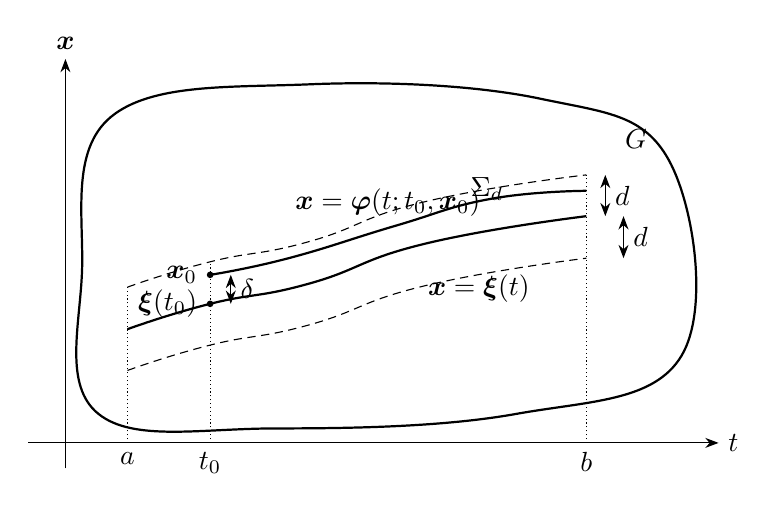
\begin{tikzpicture}[x=1.05cm,y=0.92cm,>=Stealth]
			\draw[->] (0,0.35) -- (8.35,0.35) node[right] {$t$};
			\draw[->] (0.45,0) -- (0.45,5.65) node[above] {$\vect{x}$};

			\draw[thick]
				plot[smooth cycle,tension=0.65] coordinates {
				(0.85,0.75) (0.65,2.7) (1.0,4.85) (3.4,5.3)
				(6.2,5.1) (7.75,4.25) (7.9,1.55) (5.9,0.75) (3.0,0.55)
				};
			\node at (7.35,4.55) {$G$};

			\draw[densely dashed]
				plot[smooth,tension=0.85] coordinates {
				(1.2,2.5) (2.2,2.85) (3.4,3.13) (4.8,3.68) (6.75,4.05)
				};
			\draw[densely dashed]
				plot[smooth,tension=0.85] coordinates {
				(1.2,1.35) (2.2,1.7) (3.4,1.98) (4.8,2.52) (6.75,2.9)
				};
			\draw[thick]
				plot[smooth,tension=0.85] coordinates {
				(1.2,1.92) (2.2,2.27) (3.4,2.55) (4.8,3.1) (6.75,3.48)
				};
			\node[below] at (5.45,2.8) {$\vect{x}=\vect{\xi}(t)$};
			\node at (5.55,3.85) {$\Sigma_d$};

			\draw[thick]
				plot[smooth,tension=0.8] coordinates {
				(2.2,2.67) (3.15,2.9) (4.45,3.35) (5.6,3.72) (6.75,3.83)
				};
			\node[above] at (4.35,3.34)
				{$\vect{x}=\vect{\varphi}(t;t_0,\vect{x}_0)$};

			\draw[densely dotted] (1.2,0.35) -- (1.2,2.5);
			\draw[densely dotted] (2.2,0.35) -- (2.2,2.85);
			\draw[densely dotted] (6.75,0.35) -- (6.75,4.05);
			\node[below] at (1.2,0.35) {$a$};
			\node[below] at (2.2,0.35) {$t_0$};
			\node[below] at (6.75,0.35) {$b$};

			\fill (2.2,2.27) circle (1.2pt);
			\fill (2.2,2.67) circle (1.2pt);
			\node[left] at (2.16,2.27) {$\vect{\xi}(t_0)$};
			\node[left] at (2.16,2.67) {$\vect{x}_0$};
			\draw[<->] (2.45,2.27) -- (2.45,2.67)
				node[midway,right] {$\delta$};

			\draw[<->] (6.98,3.48) -- (6.98,4.05)
				node[midway,right] {$d$};
			\draw[<->] (7.2,2.9) -- (7.2,3.48)
				node[midway,right] {$d$};
		\end{tikzpicture}
		\caption{解关于初值的整体连续依赖性}
		\label{fig:解关于初值的整体连续依赖性}
	\end{figure}

	第二步，在上述管状邻域内构造 Picard 逐次逼近函数列：
	\[
		\vect{\varphi}_0(t;t_0,\vect{x}_0)
		=\vect{x}_0+\vect{\xi}(t)-\vect{\xi}(t_0),
	\]
	\[
		\vect{\varphi}_{k+1}(t;t_0,\vect{x}_0)
		=\vect{x}_0+
		\int_{t_0}^t
		\vect{f}\bigl(
		\tau,\vect{\varphi}_k(\tau;t_0,\vect{x}_0)
		\bigr)\dd\tau.
	\]

	第三步，取
	\[
		\delta=\dfrac{1}{2}e^{-L(b-a)}d,
	\]
	显然 $0<\delta<d$。下面用归纳法证明，在 $D_\delta$ 上有
	\[
		\norm{
		\vect{\varphi}_k(t;t_0,\vect{x}_0)-\vect{\xi}(t)
		}<d,
	\]
	以及
	\[
		\norm{
		\vect{\varphi}_{k+1}(t;t_0,\vect{x}_0)
		-\vect{\varphi}_k(t;t_0,\vect{x}_0)
		}
		\leq
		\dfrac{(L\abs{t-t_0})^{k+1}}{(k+1)!}
		\norm{\vect{x}_0-\vect{\xi}(t_0)},
		\qquad k=0,1,2,\ldots.
	\]
	当 $k=0$ 时，
	\[
		\norm{
		\vect{\varphi}_0(t;t_0,\vect{x}_0)-\vect{\xi}(t)
		}
		=\norm{\vect{x}_0-\vect{\xi}(t_0)}
		\leq\delta<d.
	\]
	又有
	\begin{align*}
		&\norm{
		\vect{\varphi}_1(t;t_0,\vect{x}_0)
		-\vect{\varphi}_0(t;t_0,\vect{x}_0)
		}\\
		={}&\norm{
		\int_{t_0}^t
		\vect{f}\bigl(\tau,\vect{\varphi}_0(\tau;t_0,\vect{x}_0)\bigr)
		\dd\tau-\vect{\xi}(t)+\vect{\xi}(t_0)
		}\\
		={}&\norm{
		\int_{t_0}^t
		\left[
		\vect{f}\bigl(\tau,\vect{\varphi}_0(\tau;t_0,\vect{x}_0)\bigr)
		-\vect{f}(\tau,\vect{\xi}(\tau))
		\right]\dd\tau
		}\\
		\leq{}&L\abs{
		\int_{t_0}^t
		\norm{
		\vect{\varphi}_0(\tau;t_0,\vect{x}_0)-\vect{\xi}(\tau)
		}\dd\tau
		}\\
		={}&L\norm{\vect{x}_0-\vect{\xi}(t_0)}\abs{t-t_0}.
	\end{align*}
	所以两个估计式对 $k=0$ 成立。

	假设它们对 $k\leq s-1$ 成立，则当 $k=s$ 时，
	\begin{align*}
		&\norm{
		\vect{\varphi}_s(t;t_0,\vect{x}_0)-\vect{\xi}(t)
		}\\
		={}&\norm{
		\sum_{k=1}^s
		\bigl(
		\vect{\varphi}_k(t;t_0,\vect{x}_0)
		-\vect{\varphi}_{k-1}(t;t_0,\vect{x}_0)
		\bigr)
		+\vect{\varphi}_0(t;t_0,\vect{x}_0)-\vect{\xi}(t)
		}\\
		\leq{}&
		\sum_{k=1}^s
		\dfrac{(L\abs{t-t_0})^k}{k!}
		\norm{\vect{x}_0-\vect{\xi}(t_0)}
		+\norm{\vect{x}_0-\vect{\xi}(t_0)}\\
		\leq{}&e^{L\abs{t-t_0}}\delta
		\leq e^{L(b-a)}\delta<d.
	\end{align*}
	这就证明了第一个估计。再利用 Lipschitz 条件，与上面相同地可得
	\[
		\norm{
		\vect{\varphi}_{s+1}(t;t_0,\vect{x}_0)
		-\vect{\varphi}_s(t;t_0,\vect{x}_0)
		}
		\leq
		\dfrac{(L\abs{t-t_0})^{s+1}}{(s+1)!}
		\norm{\vect{x}_0-\vect{\xi}(t_0)},
	\]
	故第二个估计也成立。

	第四步，由上述估计，函数列
	\[
		\{\vect{\varphi}_k(t;t_0,\vect{x}_0)\}
	\]
	在 $D_\delta$ 上一致收敛。
	令其极限为 $\vect{\varphi}(t;t_0,\vect{x}_0)$，则它满足所考察的
	积分方程，因而是相应初值问题的解。又因各
	$\vect{\varphi}_k$ 连续且收敛一致，故
	$\vect{\varphi}$ 在 $D_\delta$ 上连续。唯一性由 Lipschitz 条件得到。
\end{proof}
\ref{thm:连续依赖性定理}与\ref{thm:整体连续依赖性定理}的区别，\ref{thm:整体连续依赖性定理}是\ref{thm:连续依赖性定理}的一个加强，\ref{thm:连续依赖性定理}只保证了解关于参数在初值附近的一个小区间上连续，但是\ref{thm:整体连续依赖性定理}在确保一个解存在的基础上，能够保证解在整个区间上连续。

下面进一步讨论解对参数的可微依赖性。

\begin{theorem}($C^1$ 依赖性定理)\label{thm:C1依赖性定理}
	设 $G$ 与定理 \ref{thm:连续依赖性定理} 中相同，函数
	\[
		\vect{f}:G\longrightarrow\R^n
	\]
	连续，并且关于 $\vect{x}$ 和 $\vect{\lambda}$ 具有连续的偏导数。
	则初值问题
	\[\frac{\dd \vect x}{\dd t}=\vect{f}(t,\vect x,\vect\lambda)\qquad \vect{x}(0)=0\]
	的解 $\vect{\varphi}(t,\vect{\lambda})$ 在区域
	\[
		D=\left\{
		(t,\vect{\lambda})\in\R\times\R^m:
		\abs{t}\leq h,
		\norm{\vect{\lambda}-\vect{\lambda}_0}\leq c
		\right\}
	\]
	上连续可微，其中 $h,M$ 与定理 \ref{thm:连续依赖性定理} 中相同。
\end{theorem}

\begin{proof}
	关于这个问题我们介绍两个证明方法：
	
	\textbf{法一：}第一步，初值问题等价于积分方程
	\[
		\vect{x}(t)=\int_0^t
		\vect{f}\bigl(\tau,\vect{x}(\tau),\vect{\lambda}\bigr)\dd\tau.
	\]
	构造逐次逼近函数列
	\[
		\vect{\varphi}_0(t,\vect{\lambda})=\vect{0},
	\]
	\[
		\vect{\varphi}_{k+1}(t,\vect{\lambda})
		=\int_0^t
		\vect{f}\bigl(
		\tau,\vect{\varphi}_k(\tau,\vect{\lambda}),\vect{\lambda}
		\bigr)\dd\tau.
	\]

	第二步，由于 $\vect{f}$ 关于 $\vect{x},\vect{\lambda}$ 的偏导数连续，
	且 $G$ 为有界闭集，故 $\vect{f}$ 关于 $\vect{x},\vect{\lambda}$
	均满足 Lipschitz 条件。由定理 \ref{thm:连续依赖性定理}，
	$\vect{\varphi}_k$ 在 $D$ 上一致收敛于初值问题唯一的连续解
	$\vect{\varphi}$。

	第三步，证明函数列
	\[
		\left\{
		\dfrac{\partial\vect{\varphi}_k}{\partial\vect{\lambda}}
		\right\}
	\]
	一致收敛。这里
	\[
		\dfrac{\partial\vect{\varphi}_k}
		{\partial\vect{\lambda}}
	\]
	是 $n\times m$ 矩阵。由逐次逼近公式可知，每个
	$\vect{\varphi}_k$ 都连续可微。记
	\[
		\mat{P}_k(t,\vect{\lambda})
		\mathrel{:=}
		\dfrac{\partial\vect{\varphi}_k}
		{\partial\vect{\lambda}}(t,\vect{\lambda}),
	\]
	并记
	\[
		\begin{aligned}
		\mat{A}_k(t,\vect{\lambda})
		&\mathrel{:=}
		\dfrac{\partial\vect{f}}{\partial\vect{x}}
		\bigl(t,\vect{\varphi}_k(t,\vect{\lambda}),\vect{\lambda}\bigr),\\
		\mat{B}_k(t,\vect{\lambda})
		&\mathrel{:=}
		\dfrac{\partial\vect{f}}{\partial\vect{\lambda}}
		\bigl(t,\vect{\varphi}_k(t,\vect{\lambda}),\vect{\lambda}\bigr).
		\end{aligned}
	\]
	则
	\[
		\mat{P}_{k+1}(t,\vect{\lambda})
		=\int_0^t\left[
		\mat{A}_k(\tau,\vect{\lambda})
		\mat{P}_k(\tau,\vect{\lambda})
		+\mat{B}_k(\tau,\vect{\lambda})
		\right]\dd\tau.
	\]
	根据 Cauchy 收敛准则，只需对每个固定的
	$s=1,2,\ldots$，证明函数列
	\[
		v_{k,s}(t,\vect{\lambda})\mathrel{:=}
		\norm{
		\mat{P}_{k+s}(t,\vect{\lambda})
		-\mat{P}_k(t,\vect{\lambda})
		}
	\]
	当 $k\to\infty$ 时一致趋于零。

	第四步，由于 $G$ 为有界闭集，且 $\vect{f}$ 的偏导数连续，故存在常数
	$M_1>0$，使得
	\[
		\norm{\mat{A}_k(t,\vect{\lambda})}\leq M_1,
		\qquad
		\norm{\mat{B}_k(t,\vect{\lambda})}\leq M_1,
		\qquad (t,\vect{\lambda})\in D,
	\]
	其中矩阵范数取诱导范数。注意到 $\mat{P}_0=\mat{0}$，从而
	\[
		\norm{\mat{P}_1(t,\vect{\lambda})}
		\leq M_1\abs{t}.
	\]
	由归纳法可得
	\[
		\norm{\mat{P}_k(t,\vect{\lambda})}
		\leq M_1\abs{t}
		+\dfrac{(M_1\abs{t})^2}{2!}
		+\cdots
		+\dfrac{(M_1\abs{t})^k}{k!}.
	\]
	因此
	\[
		\norm{\mat{P}_k(t,\vect{\lambda})}
		\leq\beta\mathrel{:=}e^{M_1h},
		\qquad k=1,2,\ldots.
	\]

	记
	\[
		\mat{A}(t,\vect{\lambda})
		\mathrel{:=}
		\dfrac{\partial\vect{f}}{\partial\vect{x}}
		\bigl(t,\vect{\varphi}(t,\vect{\lambda}),\vect{\lambda}\bigr).
	\]
	由上面的逐次逼近公式及矩阵范数的次乘性，有
	\[
		v_{k+1,s}(t,\vect{\lambda})
		\leq M_1\abs{\int_0^t
		v_{k,s}(\tau,\vect{\lambda})\dd\tau}
		+d_{k,s}(t,\vect{\lambda}),
	\]
	其中
	\[
	\begin{aligned}
		d_{k,s}(t,\vect{\lambda})
		={}&\norm{\int_0^t
		\bigl[\mat{A}_{k+s}(\tau,\vect{\lambda})
		-\mat{A}(\tau,\vect{\lambda})\bigr]
		\mat{P}_{k+s}(\tau,\vect{\lambda})\dd\tau}\\
		&+\norm{\int_0^t
		\bigl[\mat{A}(\tau,\vect{\lambda})
		-\mat{A}_k(\tau,\vect{\lambda})\bigr]
		\mat{P}_k(\tau,\vect{\lambda})\dd\tau}\\
		&+\norm{\int_0^t
		\bigl[\mat{B}_{k+s}(\tau,\vect{\lambda})
		-\mat{B}_k(\tau,\vect{\lambda})\bigr]\dd\tau}.
	\end{aligned}
	\]
	这里利用了
	\[
		\begin{aligned}
		\mat{A}_{k+s}\mat{P}_{k+s}-\mat{A}_k\mat{P}_k
		={}&\mat{A}(\mat{P}_{k+s}-\mat{P}_k)
		+(\mat{A}_{k+s}-\mat{A})\mat{P}_{k+s}\\
		&+(\mat{A}-\mat{A}_k)\mat{P}_k.
		\end{aligned}
	\]
	由于 $\vect{\varphi}_k$ 一致收敛于 $\vect{\varphi}$，且
	$\vect{f}$ 的偏导数连续，$\mat{A}_k$ 与 $\mat{B}_k$ 分别在
	$D$ 上一致收敛。结合 $\mat{P}_k$ 的一致有界性可知，存在
	$\varepsilon_k>0$，$\varepsilon_k\to0$，使得对任意
	$s=1,2,\ldots$，都有
	\[
		d_{k,s}(t,\vect{\lambda})\leq\varepsilon_k,
		\qquad (t,\vect{\lambda})\in D.
	\]
	因此
	\[
		v_{k+1,s}(t,\vect{\lambda})
		\leq M_1\abs{\int_0^t
		v_{k,s}(\tau,\vect{\lambda})\dd\tau}
		+\varepsilon_k.
	\]

	函数 $v_{k,s}$ 连续且非负，由前面的估计有
	\[
		v_{k,s}(t,\vect{\lambda})\leq2\beta.
	\]
	因此
	\[
		v_{k+1,s}(t,\vect{\lambda})
		\leq2\beta M_1\abs{t}+\varepsilon_k.
	\]
	归纳可得
	\[
		v_{k+m,s}(t,\vect{\lambda})
		\leq
		2\beta\dfrac{(M_1\abs{t})^m}{m!}
		+\sum_{j=0}^{m-1}
		\varepsilon_{k+m-1-j}
		\dfrac{(M_1\abs{t})^j}{j!}.
	\]
	令
	\[
		E_k\mathrel{:=}\sup\{\varepsilon_k,\varepsilon_{k+1},\ldots\},
	\]
	则 $E_k\downarrow0$，并且
	\[
		v_{k+m,s}(t,\vect{\lambda})
		\leq
		2\beta\dfrac{(M_1\abs{t})^m}{m!}
		+e^{M_1h}E_k.
	\]
	任给 $\varepsilon>0$，取充分大的 $N$，则当
	$m>N/2$ 且 $k>N/2$ 时，上式右端的两项分别小于
	$\varepsilon/2$。因此当 $k>N$ 时，
	\[
		v_{k,s}(t,\vect{\lambda})<\varepsilon,
	\]
	这就证明了函数列 $\{\mat{P}_k\}$ 在 $D$ 上一致收敛。

	第五步，由函数列及其偏导数的一致收敛性，
	\[
		\lim_{k\to\infty}
		\dfrac{\partial\vect{\varphi}_k}{\partial\vect{\lambda}}
		=\dfrac{\partial\vect{\varphi}}{\partial\vect{\lambda}},
	\]
	并且 $\dfrac{\partial\vect{\varphi}}
	{\partial\vect{\lambda}}$ 连续。另一方面，
	\[
		\dfrac{\dd}{\dd t}\vect{\varphi}(t,\vect{\lambda})
		=\vect{f}\bigl(
		t,\vect{\varphi}(t,\vect{\lambda}),\vect{\lambda}
		\bigr)
	\]
	在 $D$ 上连续。因此 $\vect{\varphi}(t,\vect{\lambda})$ 关于
	$(t,\vect{\lambda})$ 连续可微。
	
	\textbf{法二：利用增量方程与Gronwall估计。}
先由线性方程确定参数导数应满足的方程，再证明解的增量与该线性近似之差为高阶小量。
记
\[
 A(t,\lambda)=D_xf(t,\varphi(t,\lambda),\lambda),\qquad
 B(t,\lambda)=D_\lambda f(t,\varphi(t,\lambda),\lambda).
\]
这里用 $f,\varphi,\lambda$ 简记原来的向量函数与参数。由线性方程的存在唯一性，矩阵初值问题
\[
 Z'=AZ+B,\qquad Z(0,\lambda)=0
\]
有唯一解。其列分别满足线性非齐次方程；由已经证明的连续依赖性，$Z$ 关于 $(t,\lambda)$ 连续。

对参数增量 $\Delta\lambda$，记相应的解的增量为
\[
 \Delta x(t)=\varphi(t,\lambda+\Delta\lambda)-\varphi(t,\lambda).
\]
连续依赖性使它在固定紧时间段上一致趋于零。对 $f$ 使用带积分余项的一阶展开，得到
\begin{align*}
 (\Delta x)'&=(A+E_1)\Delta x+(B+E_2)\Delta\lambda,\\
 \Delta x(0)&=0,
\end{align*}
其中 $E_1,E_2$ 分别为 $n\times n,n\times m$ 矩阵，并且
\[
 \sup_{|t|\leq h}\bigl(\|E_1\|+\|E_2\|\bigr)\longrightarrow0
 \qquad(\Delta\lambda\to0).
\]
这一一致性来自 $D_xf,D_\lambda f$ 在所考察紧邻域上的一致连续性。

令 $u=\Delta x-Z\Delta\lambda$。将上式与 $Z'=AZ+B$ 相减，得
\[
 u'=(A+E_1)u+(E_1Z+E_2)\Delta\lambda,\qquad u(0)=0.
\]
取常数 $N$ 控制 $\|A\|$，并以 $\eta(\Delta\lambda)\to0$ 同时控制
$\|E_1\|$ 和 $\|E_1Z+E_2\|$。积分后使用 Gronwall 不等式，正负时间分别估计，均得到
\[
 \|u(t)\|\leq h\eta(\Delta\lambda)
 e^{(N+\eta(\Delta\lambda))h}\|\Delta\lambda\|,
 \qquad |t|\leq h.
\]
因此
\[
 \sup_{|t|\leq h}
 \frac{\|\varphi(t,\lambda+\Delta\lambda)-\varphi(t,\lambda)-Z(t,\lambda)\Delta\lambda\|}
 {\|\Delta\lambda\|}\longrightarrow0.
\]
所以 $D_\lambda\varphi=Z$。由 $Z$ 的连续性，参数导数连续；又
$\partial_t\varphi=f(t,\varphi,\lambda)$ 连续，从而得到所需的联合 $C^1$ 依赖性。
\end{proof}

\begin{corollary}\label{cor:解对初值和参数的偏导方程}
	设 $x,\lambda$ 均为一维变量，记初值问题的解为
	$\varphi(t;t_0,x_0,\lambda)$。根据定理
	\ref{thm:C1依赖性定理}，有以下结论：

	$z\mathrel{:=}\partial\varphi/\partial t_0$ 满足
	\[
		\dfrac{\dd z}{\dd t}
		=\dfrac{\partial f}{\partial x}
		\bigl(t,\varphi(t;t_0,x_0,\lambda),\lambda\bigr)z,
		\qquad
		z(t_0)=-f(t_0,x_0,\lambda).
	\]

	$z\mathrel{:=}\partial\varphi/\partial x_0$ 满足
	\[
		\dfrac{\dd z}{\dd t}
		=\dfrac{\partial f}{\partial x}
		\bigl(t,\varphi(t;t_0,x_0,\lambda),\lambda\bigr)z,
		\qquad
		z(t_0)=1.
	\]

	$z\mathrel{:=}\partial\varphi/\partial\lambda$ 满足
	\[
		\dfrac{\dd z}{\dd t}
		=\dfrac{\partial f}{\partial x}
		\bigl(t,\varphi(t;t_0,x_0,\lambda),\lambda\bigr)z
		+\dfrac{\partial f}{\partial\lambda}
		\bigl(t,\varphi(t;t_0,x_0,\lambda),\lambda\bigr),
		\qquad
		z(t_0)=0.
	\]
\end{corollary}
\begin{proposition}[初值导数的矩阵变分方程]\label{prop:matrix-variation}
设有限维方程 $x'=f(t,x)$ 的右端 $f$ 连续，且偏导矩阵 $D_xf$ 存在并连续，记解为 $\varphi(t;t_0,\xi)$。
在解共同存在的区间内，矩阵
\[
 Z(t)=D_\xi\varphi(t;t_0,\xi)
\]
满足
\[
 Z'=D_xf(t,\varphi(t;t_0,\xi))Z,\qquad Z(t_0)=I.
\]
\end{proposition}
\begin{proof}
本章解的依赖性一节所用的平移把初值 $\xi$ 变成参数，因此 $C^1$ 依赖性定理保证这个导数存在且连续。
对积分方程
\[
 \varphi(t;t_0,\xi)=\xi+\int_{t_0}^t f(s,\varphi(s;t_0,\xi))\,ds
\]
关于 $\xi$ 求导。在固定紧时间段内，相关导数连续，可交换参数微分与积分，得到
\[
 Z(t)=I+\int_{t_0}^tD_xf(s,\varphi(s;t_0,\xi))Z(s)\,ds.
\]
再对 $t$ 求导即得方程，取 $t=t_0$ 得到初始矩阵 $I$。
该矩阵方程逐列是一阶线性初值问题，故解唯一。
\end{proof}

\begin{corollary}($C^r$ 依赖性推论)\label{cor:Cr依赖性推论}
	设 $r\in\N$，$r\geq1$，$G$ 与定理
	\ref{thm:连续依赖性定理} 中相同，函数
	\[
	\vect{f}:G\longrightarrow\R^n
	\]
	连续，并且关于 $\vect{x}$ 和 $\vect{\lambda}$ 具有直到 $r$ 阶的
	连续偏导数，即所有总阶数不超过 $r$ 的关于
	$\vect{x},\vect{\lambda}$ 的混合偏导数均存在且在 $G$ 上连续。
	则初值问题
	\[
	\frac{\dd\vect{x}}{\dd t}
	=
	\vect{f}(t,\vect{x},\vect{\lambda}),
	\qquad
	\vect{x}(0)=\vect{0}
	\]
	的解 $\vect{\varphi}(t,\vect{\lambda})$ 在区域
	\[
	D=
	\left\{
	(t,\vect{\lambda})\in\R\times\R^m:
	\abs{t}\leq h,\;
	\norm{\vect{\lambda}-\vect{\lambda}_0}\leq c
	\right\}
	\]
	上关于参数 $\vect{\lambda}$ 连续 $r$ 阶可微，其中 $h,M$
	与定理 \ref{thm:连续依赖性定理} 中相同。
	
	若进一步 $\vect{f}$ 关于
	$t,\vect{x},\vect{\lambda}$ 具有直到 $r$ 阶的连续偏导数，
	则 $\vect{\varphi}(t,\vect{\lambda})$ 在 $D$ 上关于
	$(t,\vect{\lambda})$ 连续 $r$ 阶可微。
\end{corollary}

\begin{proof}
	记
	\[
	\vect{\lambda}
	=
	(\lambda_1,\lambda_2,\ldots,\lambda_m).
	\]
	对多重指标
	\[
	\alpha=(\alpha_1,\alpha_2,\ldots,\alpha_m)\in\N_0^m
	\]
	记
	\[
	\abs{\alpha}
	=
	\alpha_1+\alpha_2+\cdots+\alpha_m,
	\]
	以及
	\[
	\partial_{\vect{\lambda}}^\alpha
	=
	\frac{
		\partial^{\abs{\alpha}}
	}{
		\partial\lambda_1^{\alpha_1}
		\partial\lambda_2^{\alpha_2}
		\cdots
		\partial\lambda_m^{\alpha_m}
	}.
	\]
	
	下面对参数偏导数的阶数作归纳。
	
	当 $\abs{\alpha}=1$ 时，结论就是定理
	\ref{thm:C1依赖性定理}，因此
	\[
	\partial_{\vect{\lambda}}^\alpha
	\vect{\varphi}(t,\vect{\lambda})
	\]
	存在并且在 $D$ 上连续。
	
	假设对某个 $k$，$1\leq k<r$，所有满足
	\[
	\abs{\beta}\leq k
	\]
	的多重指标 $\beta$，都有
	\[
	\partial_{\vect{\lambda}}^\beta
	\vect{\varphi}(t,\vect{\lambda})
	\]
	存在并且在 $D$ 上连续。下面证明所有 $k+1$ 阶参数偏导数
	也存在且连续。
	
	记
	\[
	\mat{A}(t,\vect{\lambda})
	\mathrel{:=}
	\frac{\partial\vect{f}}{\partial\vect{x}}
	\bigl(
	t,\vect{\varphi}(t,\vect{\lambda}),\vect{\lambda}
	\bigr).
	\]
	由一阶情形，
	\[
	\vect{z}_j
	\mathrel{:=}
	\frac{\partial\vect{\varphi}}{\partial\lambda_j}
	\]
	满足
	\[
	\frac{\dd\vect{z}_j}{\dd t}
	=
	\mat{A}(t,\vect{\lambda})\vect{z}_j
	+
	\frac{\partial\vect{f}}{\partial\lambda_j}
	\bigl(
	t,\vect{\varphi}(t,\vect{\lambda}),\vect{\lambda}
	\bigr),
	\qquad
	\vect{z}_j(0,\vect{\lambda})=\vect{0}.
	\]
	
	一般地，由归纳假设以及链式法则，对于任意满足
	$1\leq\abs{\beta}\leq k$ 的多重指标 $\beta$，记
	\[
	\vect{z}_{\beta}
	\mathrel{:=}
	\partial_{\vect{\lambda}}^\beta
	\vect{\varphi},
	\]
	则 $\vect{z}_{\beta}$ 满足形如
	\[
	\frac{\dd\vect{z}_{\beta}}{\dd t}
	=
	\mat{A}(t,\vect{\lambda})\vect{z}_{\beta}
	+
	\vect{F}_{\beta}(t,\vect{\lambda}),
	\qquad
	\vect{z}_{\beta}(0,\vect{\lambda})=\vect{0}
	\]
	的线性非齐次方程，其中
	$\vect{F}_{\beta}$ 仅由
	$\vect{f}$ 的不超过 $\abs{\beta}$ 阶的
	$\vect{x},\vect{\lambda}$ 偏导数以及
	\[
	\partial_{\vect{\lambda}}^\gamma
	\vect{\varphi},
	\qquad
	\abs{\gamma}<\abs{\beta},
	\]
	经过有限次加法和乘法构成。
	
	现在任取满足
	\[
	\abs{\alpha}=k+1
	\]
	的多重指标 $\alpha$。取某个 $j$ 使得
	$\alpha_j\geq1$，并令
	\[
	\beta=\alpha-\vect{e}_j,
	\]
	其中 $\vect{e}_j$ 为第 $j$ 个坐标方向的单位多重指标，
	则 $\abs{\beta}=k$。
	
	由归纳假设，
	\[
	\vect{z}_{\beta}
	=
	\partial_{\vect{\lambda}}^\beta
	\vect{\varphi}
	\]
	存在且连续，并且满足
	\[
	\frac{\dd\vect{z}_{\beta}}{\dd t}
	=
	\mat{A}\vect{z}_{\beta}
	+
	\vect{F}_{\beta}.
	\]
	由于 $\vect{f}$ 关于
	$\vect{x},\vect{\lambda}$ 具有直到 $k+1$ 阶的连续偏导数，
	再结合归纳假设可知
	\[
	\mat{A}(t,\vect{\lambda}),
	\qquad
	\vect{F}_{\beta}(t,\vect{\lambda})
	\]
	关于 $\lambda_j$ 均连续可微。
	
	形式上对上式关于 $\lambda_j$ 求偏导，应有
	\[
	\frac{\dd\vect{z}_{\alpha}}{\dd t}
	=
	\mat{A}\vect{z}_{\alpha}
	+
	\frac{\partial\mat{A}}{\partial\lambda_j}
	\vect{z}_{\beta}
	+
	\frac{\partial\vect{F}_{\beta}}{\partial\lambda_j},
	\qquad
	\vect{z}_{\alpha}(0,\vect{\lambda})=\vect{0},
	\]
	其中
	\[
	\vect{z}_{\alpha}
	\mathrel{:=}
	\partial_{\vect{\lambda}}^\alpha
	\vect{\varphi}.
	\]
	上式右端连续，因此这个线性初值问题在
	$\abs{t}\leq h$ 上存在唯一解。
	
	下面证明这个解确实等于
	\[
	\frac{\partial\vect{z}_{\beta}}{\partial\lambda_j}.
	\]
	令参数 $\lambda_j$ 有改变量 $\Delta\lambda_j$，并记
	\[
	\Delta\vect{z}_{\beta}
	=
	\vect{z}_{\beta}
	(t,\vect{\lambda}+\Delta\lambda_j\vect{e}_j)
	-
	\vect{z}_{\beta}(t,\vect{\lambda}).
	\]
	再令
	\[
	\Delta\vect{u}
	=
	\Delta\vect{z}_{\beta}
	-
	\vect{z}_{\alpha}(t,\vect{\lambda})
	\Delta\lambda_j.
	\]
	由 $\mat{A}$ 与 $\vect{F}_{\beta}$ 关于 $\lambda_j$
	连续可微，利用中值公式可将相应增量写成
	\[
	\Delta\mat{A}
	=
	\left(
	\frac{\partial\mat{A}}{\partial\lambda_j}
	+\mat{\varepsilon}_1
	\right)\Delta\lambda_j,
	\]
	以及
	\[
	\Delta\vect{F}_{\beta}
	=
	\left(
	\frac{\partial\vect{F}_{\beta}}{\partial\lambda_j}
	+\vect{\varepsilon}_2
	\right)\Delta\lambda_j,
	\]
	其中当 $\Delta\lambda_j\to0$ 时，
	\[
	\norm{\mat{\varepsilon}_1}\longrightarrow0,
	\qquad
	\norm{\vect{\varepsilon}_2}\longrightarrow0,
	\]
	并且上述收敛在 $D$ 上一致。
	
	将增量方程与 $\vect{z}_{\alpha}$ 所满足的方程相减，
	可得
	\[
	\Delta\vect{u}(t)
	=
	\int_0^t
	\left[
	\mat{A}(\tau,\vect{\lambda})
	\Delta\vect{u}(\tau)
	+
	\vect{\varepsilon}
	(\tau,\vect{\lambda},\Delta\lambda_j)
	\Delta\lambda_j
	\right]\dd\tau,
	\]
	其中
	\[
	\sup_D
	\norm{
		\vect{\varepsilon}
		(\tau,\vect{\lambda},\Delta\lambda_j)
	}
	\longrightarrow0
	\qquad
	(\Delta\lambda_j\to0).
	\]
	
	由于 $\mat{A}$ 在 $D$ 上连续，故存在常数 $N>0$，
	使得
	\[
	\norm{\mat{A}(t,\vect{\lambda})}\leq N.
	\]
	于是
	\[
	\norm{\Delta\vect{u}(t)}
	\leq
	N
	\abs{
		\int_0^t
		\norm{\Delta\vect{u}(\tau)}
		\dd\tau
	}
	+
	h\varepsilon
	\abs{\Delta\lambda_j},
	\]
	其中 $\varepsilon\to0$ 当
	$\Delta\lambda_j\to0$。
	
	由 Gronwall 不等式，
	\[
	\norm{\Delta\vect{u}(t)}
	\leq
	h\varepsilon
	e^{Nh}
	\abs{\Delta\lambda_j}.
	\]
	因此
	\[
	\lim_{\Delta\lambda_j\to0}
	\frac{
		\norm{
			\Delta\vect{z}_{\beta}
			-
			\vect{z}_{\alpha}
			\Delta\lambda_j
		}
	}{
		\abs{\Delta\lambda_j}
	}
	=0.
	\]
	这说明
	\[
	\frac{\partial\vect{z}_{\beta}}{\partial\lambda_j}
	=
	\vect{z}_{\alpha},
	\]
	即
	\[
	\partial_{\vect{\lambda}}^\alpha
	\vect{\varphi}
	\]
	存在。又由于 $\vect{z}_{\alpha}$ 是系数和非齐次项均连续的
	线性方程的解，由连续依赖性定理可知
	$\vect{z}_{\alpha}$ 在 $D$ 上连续。
	
	故所有 $k+1$ 阶参数偏导数均存在且连续。
	由数学归纳法，
	$\vect{\varphi}(t,\vect{\lambda})$ 关于
	$\vect{\lambda}$ 连续 $r$ 阶可微。
	
	最后，若 $\vect{f}$ 关于
	$t,\vect{x},\vect{\lambda}$ 具有直到 $r$ 阶的连续偏导数，
	则
	\[
	\frac{\partial\vect{\varphi}}{\partial t}
	=
	\vect{f}
	\bigl(
	t,\vect{\varphi}(t,\vect{\lambda}),\vect{\lambda}
	\bigr).
	\]
	已经证明 $\vect{\varphi}$ 关于 $\vect{\lambda}$
	具有直到 $r$ 阶连续偏导数。再对上式关于
	$t,\vect{\lambda}$ 逐次求偏导，并利用链式法则，
	可依次得到所有总阶数不超过 $r$ 的含 $t$ 的混合偏导数
	均存在且连续。因此
	\[
	\vect{\varphi}\in C^r(D).
	\]
\end{proof}

\section{局部逆与沿解移动的坐标}\label{sec:inverse-moving-coordinates}
前面已经证明解对初值和参数的 $C^1$、$C^r$ 依赖性。下面先用压缩映射定理证明局部逆的存在性，再通过沿已知解的坐标变换消去方程中的常数项和线性项。
局部逆的证明使用第~\ref{sec:picard-contraction}~节的压缩映射定理。

\begin{definition}[赋范空间、Banach 空间与有界算子]\label{def:banach-operator}
向量空间 $X$ 上的范数满足正定性、$\|ax\|=|a|\|x\|$ 及三角不等式；
由距离 $d(x,y)=\|x-y\|$ 得到的空间称赋范空间。若此距离下每个 Cauchy 列都收敛，称 Banach 空间。
线性映射 $T:X\to Y$ 有界，是指存在 $C$ 使 $\|Tx\|\leq C\|x\|$；其算子范数为
\[
 \|T\|=\sup_{\|x\|\leq1}\|Tx\|.
\]
它满足 $\|Tx\|\leq\|T\|\|x\|$ 与 $\|ST\|\leq\|S\|\|T\|$。
线性有界等价于连续：有界估计直接保证连续；反之在零点使用连续性，再缩放向量即得有界估计。
\end{definition}
\begin{lemma}[Neumann 级数]\label{lem:neumann-series}
若 $X$ 为 Banach 空间，$T:X\to X$ 线性有界且 $\|T\|<1$，则
\[
 (I-T)^{-1}=\sum_{j=0}^\infty T^j,
 \qquad\|(I-T)^{-1}\|\leq\frac1{1-\|T\|}.
\]
\end{lemma}
\begin{proof}
对每个 $x$，级数各项的范数由 $\|T\|^j\|x\|$ 控制，故由完备性收敛，记其和为 $Sx$。
这一估计同时证明 $S$ 线性有界。有限和满足
$(I-T)\sum_{j=0}^mT^j=\sum_{j=0}^mT^j(I-T)=I-T^{m+1}$。
令 $m\to\infty$，右边趋于 $I$，所以 $S$ 是双侧逆，范数估计由几何级数得到。
\end{proof}

\begin{theorem}[由压缩映射得到局部逆]\label{thm:local-inverse}
若 $F\in C^1$，且 $DF(x_0)$ 可逆，则 $F$ 在 $x_0$ 附近有 $C^1$ 局部逆。
\end{theorem}
\begin{proof}
先平移自变量和函数值，使所考察的点及其像均为原点，再左乘 $DF(x_0)^{-1}$，只需研究
$F(0)=0,DF(0)=I$ 的情形。写 $F(x)=x+R(x)$，则 $R(0)=0,DR(0)=0$。
由 $DR$ 连续，可取闭球 $B_r$，使其中 $\|DR\|\leq\theta<1$。
球的凸性与微积分中值估计给出
\[
 |R(x)-R(z)|\leq\theta|x-z|,
\]
特别地 $|R(x)|\leq\theta r$。

给定 $|y|<(1-\theta)r$，定义 $A_y(x)=y-R(x)$。
于是 $|A_y(x)|\leq|y|+\theta r\leq r$，且其压缩常数为 $\theta$。
因此存在唯一 $G(y)\in B_r$ 满足 $G(y)+R(G(y))=y$。
对 $y,z$ 的不动点方程相减，得到
\[
 |G(y)-G(z)|\leq|y-z|+\theta|G(y)-G(z)|,
\]
所以 $G$ 为 Lipschitz 连续，常数不超过 $(1-\theta)^{-1}$。

还要证明逆可微。固定 $y$，令 $x=G(y)$、$u=G(y+v)-G(y)$。
由刚得的界，$|u|\leq(1-\theta)^{-1}|v|$。
Taylor 公式给出 
\[
 v=F(x+u)-F(x)=DF(x)u+o(|u|).
\]
$DF(x)=I+DR(x)$ 可逆，其逆由收敛 Neumann 级数给出，故
\[
 u=DF(x)^{-1}v+o(|v|).
\]
于是 
\[
 DG(y)=DF(G(y))^{-1}.
\]
右端连续，所以 $G\in C^1$；而 $F$ 在小球内的单射性还可由
$|F(x)-F(z)|\geq(1-\theta)|x-z|$ 直接验证。
这给出了局部互逆的两个映射。
\end{proof}

\paragraph{沿解移动坐标与消去线性部分。}
设 $\varphi$ 是已知解，令 $x=\varphi(t)+\xi$，则新的右端在 $\xi=0$ 处为零。
令 $A(t)=D_xf(t,\varphi(t))$，写新方程为
\[
 \dot\xi=A(t)\xi+R(t,\xi),
\]
其中 $R(t,\xi)=o(|\xi|)$。
若 $X'=A(t)X$、$X(t_0)=I$，令 $\xi=X(t)\eta$，则
\[
 \dot\eta=X(t)^{-1}R(t,X(t)\eta).
\]
新方程在 $\eta=0$ 的常数项和线性项同时为零。
由近似解 $\eta(t)\equiv\eta_0$ 的积分残差
$o(|\eta_0|)$，结合前述误差估计，得到相应的解满足
\[
 \eta(t)=\eta_0+o(|\eta_0|).
\]
回到原坐标，即得解对初值的导数为 $X(t)$，这与本章
命题~\ref{prop:matrix-variation} 一致。

\setchapterimage{figure/Chapter6封面图}
\setchapterintro{}
\chapter{定性理论初步}\label{chap:qualitative}

\section{动力系统概念}\label{sec:动力系统概念}

在上一章研究的微分方程组中，如果右端函数只依赖于状态变量
$\vect{x}$，即
\[
	\dfrac{\dd\vect{x}}{\dd t}=\vect{f}(\vect{x}),
	\qquad \vect{x}\in\R^n,
\]
则称它为\textbf{自治微分方程组}或\textbf{自治系统}。

\begin{definition}\label{def:相空间向量场与轨道}
	状态变量 $\vect{x}$ 所在的空间 $\R^n$ 称为自治系统的
	\textbf{相空间}；相空间中每一点 $\vect{x}$ 处的向量
	$\vect{f}(\vect{x})$ 构成自治系统的\textbf{向量场}；解曲线在
	相空间中的像称为自治系统的\textbf{轨道}。
\end{definition}

\begin{definition}\label{def:平衡点与闭轨}
	若 $\vect{x}_0\in\R^n$ 满足
	\[
		\vect{f}(\vect{x}_0)=\vect{0},
	\]
	则称 $\vect{x}_0$ 为自治系统的\textbf{平衡点}，也称为
	\textbf{奇点}。此时从 $\vect{x}_0$ 出发的解是常值解
	$\vect{x}(t)\equiv\vect{x}_0$。

	若非常值解 $\vect{\varphi}(t;t_0,\vect{x}_0)$ 是 $t$ 的周期函数，
	则它在相空间中的轨道是一条闭曲线，称为\textbf{闭轨}或
	\textbf{周期轨}。
\end{definition}

自治系统的解具有以下基本性质，这些性质是非自治系统所不具备的。

\begin{proposition}\label{thm:自治系统解的基本性质}
	设自治系统满足解的存在唯一性条件，并且每个解的存在区间均为
	$(-\infty,+\infty)$。则其解
	$\vect{\varphi}(t;t_0,\vect{x}_0)$ 具有下列性质：

	\textnormal{(i)} \textbf{积分曲线的平移不变性}：对任意常数
	$\tau$，函数
	$\vect{\varphi}(t+\tau;t_0,\vect{x}_0)$ 也是该自治系统的解，且
	\[
		\vect{\varphi}(t-t_0;0,\vect{x}_0)
		\equiv\vect{\varphi}(t;t_0,\vect{x}_0).
	\]
	因此，初始时刻取为 $0$ 的解
	\[
		\vect{\varphi}(t,\vect{x}_0)
		\mathrel{:=}\vect{\varphi}(t;0,\vect{x}_0)
	\]
	的性质代表了该自治系统一切解的性质。

	\textnormal{(ii)} \textbf{群性质}：
	\[
		\vect{\varphi}(0,\vect{x}_0)=\vect{x}_0,
		\qquad
		\vect{\varphi}\bigl(t,\vect{\varphi}(s,\vect{x}_0)\bigr)
		=\vect{\varphi}(t+s,\vect{x}_0),
		\qquad \forall t,s\in\R.
	\]

	\textnormal{(iii)} \textbf{轨道唯一性}：通过相空间中的任意一点，
	只有该自治系统唯一的一条轨道。
\end{proposition}

\begin{proof}
	性质 \textnormal{(i)} 的前半部分可由自治系统直接验证。对任意
	$(t_0,\vect{x}_0)$，函数
	\[
		\vect{x}=\vect{\varphi}(t-t_0;0,\vect{x}_0)
	\]
	也是自治系统的解，并且与
	$\vect{\varphi}(t;t_0,\vect{x}_0)$ 满足同一初值条件
	$\vect{x}(t_0)=\vect{x}_0$。由解的唯一性，必有
	\[
		\vect{\varphi}(t;t_0,\vect{x}_0)
		\equiv\vect{\varphi}(t-t_0;0,\vect{x}_0).
	\]

	由性质 \textnormal{(i)}，
	$\vect{\varphi}\bigl(t,\vect{\varphi}(s,\vect{x}_0)\bigr)$ 和
	$\vect{\varphi}(t+s,\vect{x}_0)$ 都是自治系统的解。令 $t=0$，有
	\[
		\vect{\varphi}\bigl(0,\vect{\varphi}(s,\vect{x}_0)\bigr)
		=\vect{\varphi}(s,\vect{x}_0),
	\]
	故这两个解满足相同的初值条件。由解的唯一性，
	\[
		\vect{\varphi}\bigl(t,\vect{\varphi}(s,\vect{x}_0)\bigr)
		=\vect{\varphi}(t+s,\vect{x}_0),
	\]
	性质 \textnormal{(ii)} 得证。

	对于性质 \textnormal{(iii)}，设由
	$\vect{\varphi}(t-t_0,\vect{x}_0)$ 和
	$\vect{\varphi}(t-\widetilde{t}_0,\widetilde{\vect{x}}_0)$ 所确定的
	两条轨道相交，则存在 $t_1,t_2$，使得
	\[
		\vect{\varphi}(t_1-t_0,\vect{x}_0)
		=\vect{\varphi}(t_2-\widetilde{t}_0,\widetilde{\vect{x}}_0).
	\]
	由群性质，
	\begin{align*}
		\vect{\varphi}(t-t_0,\vect{x}_0)
		&=\vect{\varphi}\bigl(
		t-t_1,\vect{\varphi}(t_1-t_0,\vect{x}_0)
		\bigr)\\
		&=\vect{\varphi}\bigl(
		t-t_1,\vect{\varphi}(t_2-\widetilde{t}_0,
		\widetilde{\vect{x}}_0)
		\bigr)\\
		&=\vect{\varphi}
		(t-t_1+t_2-\widetilde{t}_0,\widetilde{\vect{x}}_0).
	\end{align*}
	这表明两解在相空间中由相同的几何点组成，即两条轨道重合。因此，
	自治系统的两条轨道要么完全重合，要么永不相交。
\end{proof}

上述定理假设自治系统的每个解都在 $(-\infty,+\infty)$ 上存在。
若原自治系统不满足这一条件，可以考虑归一化系统
\[
	\dfrac{\dd\vect{x}}{\dd t}
	=\dfrac{\vect{f}(\vect{x})}
	{\sqrt{1+\norm{\vect{f}(\vect{x})}^2}}.
\]
原自治系统与归一化系统在相空间中具有相同的轨道。另一方面，归一化
系统的右端满足
\[
	\norm{
	\dfrac{\vect{f}(\vect{x})}
	{\sqrt{1+\norm{\vect{f}(\vect{x})}^2}}
	}\leq1,
\]
所以由定理 \ref{thm:解的延拓定理}，归一化系统的解的存在区间为
$(-\infty,+\infty)$。因此，在研究自治系统的轨道结构时，不妨假设
它的解都在 $(-\infty,+\infty)$ 上存在。

下面说明两个系统具有相同轨道。设
$\vect{x}=\vect{\psi}(t)$ 是归一化系统满足初值条件
$\vect{x}(0)=\vect{x}_0$ 的解，令
\[
	s=w(t)\mathrel{:=}
	\int_0^t
	\dfrac{\dd\tau}
	{\sqrt{1+\norm{\vect{f}(\vect{\psi}(\tau))}^2}}.
\]
由于 $w'(t)>0$，故 $s=w(t)$ 有光滑的反函数 $t=w^{-1}(s)$。令
\[
	\vect{\phi}(s)=\vect{\psi}\bigl(w^{-1}(s)\bigr),
\]
则
\[
	\dfrac{\dd\vect{\phi}}{\dd s}
	=\dfrac{\vect{\psi}'(t)}{w'(t)}
	=\vect{f}(\vect{\phi}(s)),
	\qquad
	\vect{\phi}(0)=\vect{x}_0.
\]
所以，若把原自治系统的自变量记为 $s$，则
$\vect{x}=\vect{\phi}(s)$ 是它满足初值条件
$\vect{x}(0)=\vect{x}_0$ 的解。从几何上看，
$\vect{\phi}(s)$ 与 $\vect{\psi}(t)$ 在相空间中表示同一条曲线，只是
参数表示不同。这就证明了两个系统具有相同的轨道。

现在将定理 \ref{thm:自治系统解的基本性质} 中解的性质归纳起来。简记
\[
	\vect{\varphi}^{t}(\vect{x})
	\mathrel{:=}\vect{\varphi}(t,\vect{x}),
\]
则单参数变换族
$\{\vect{\varphi}^{t}:t\in\R\}$ 满足：

\textnormal{(1)} $\vect{\varphi}^{t}:\R^n\to\R^n$ 是连续的；

\textnormal{(2)} $\vect{\varphi}^{0}$ 为恒同变换，即
$\vect{\varphi}^{0}(\vect{x})\equiv\vect{x}$；

\textnormal{(3)}
$\vect{\varphi}^{t}\circ\vect{\varphi}^{s}
=\vect{\varphi}^{t+s}$。

\begin{definition}\label{def:动力系统与流}
	满足上述三条性质的单参数连续变换族
	$\{\vect{\varphi}^{t}:t\in\R\}$ 称为一个\textbf{动力系统}，
	也称为\textbf{流}。由于参数 $t$ 在 $\R$ 中连续取值，它也称为
	\textbf{连续动力系统}。若参数 $t$ 仅在 $\Z$ 中取值，则称
	$\{\vect{\varphi}^{t}:t\in\Z\}$ 为\textbf{离散动力系统}。
\end{definition}

对于非自治系统
\[
	\dfrac{\dd\vect{x}}{\dd t}=\vect{f}(t,\vect{x}),
\]
上述性质一般不再成立。然而，在高一维的相空间中仍可以定义相应的
动力系统。事实上，在 $(\vect{x},\theta)$ 所在的相空间
$\R^n\times\R$ 上考虑自治系统
\[
	\begin{cases}
		\dfrac{\dd\vect{x}}{\dd t}=\vect{f}(\theta,\vect{x}),\\[6pt]
		\dfrac{\dd\theta}{\dd t}=1.
	\end{cases}
\]
该系统与原非自治系统等价，称为原系统的\textbf{扭扩系统}
（suspension system）。

\subsection*{相流的体积变化}
\phantomsection\label{sec:nonlinear-volume}
由命题~\ref{prop:matrix-variation}，相流对初值的导数满足线性变分方程。将定理~\ref{thm:Wronski判别与Liouville公式} 应用于该方程，即可求出相流的 Jacobi 行列式，进而讨论体积的变化。
\begin{definition}
Euclidean 空间上 $C^1$ 向量场的散度定义为
$\operatorname{div}v=\sum_i\partial_i v_i=\operatorname{tr}Dv$。
若 $D$ 是初始区域，记 $D(t)=\varphi^t(D)$，$V(t)$ 为其体积。
以下假定 $D$ 有界且闭包上的流在所考察时间段内存在。
\end{definition}
\begin{theorem}[非线性 Liouville 公式]\label{thm:nonlinear-liouville}
\[
 \det D\varphi^t(x)
 =\exp\int_0^t\operatorname{div}v(\varphi^s(x))\,ds,
 \qquad V'(t)=\int_{D(t)}\operatorname{div}v(y)\,dy.
\]
散度为零时，相流保持体积。
\end{theorem}
\begin{proof}
固定初值 $x$，令 $Z(t)=D\varphi^t(x)$。命题~\ref{prop:matrix-variation} 给出
\[
 Z'(t)=Dv(\varphi^t(x))Z(t),\qquad Z(0)=I.
\]
这是系数连续的线性矩阵方程。应用线性 Liouville 公式，得到
\[
 J(t,x):=\det Z(t)
 =\exp\left(\int_0^t\operatorname{tr}Dv(\varphi^s(x))\,ds\right)>0.
\]
流的逆是反向时间流，故 $\varphi^t$ 在所考察区域上为微分同胚。
换元公式因而给出 
\[
 V(t)=\displaystyle\int_DJ(t,x)\,dx,
\]
这里不必再对行列式取绝对值。
对上式求导，有
\[
 \partial_tJ(t,x)=\operatorname{div}v(\varphi^t(x))J(t,x).
\]
由于初值闭包和时间段紧，右端连续且一致有界，可在积分号下求导。因此
\begin{align*}
 V'(t)&=\int_D\operatorname{div}v(\varphi^t(x))J(t,x)\,dx\\
 &=\int_{D(t)}\operatorname{div}v(y)\,dy.
\end{align*}
若散度恒为零，则 $J=1$，从而每个这样的区域都保持体积。
\end{proof}

\section{Lyapunov 稳定性}\label{sec:Lyapunov稳定性}

考虑微分方程组
\[
	\dfrac{\dd\vect{x}}{\dd t}=\vect{f}(t,\vect{x}),
\]
设 $\vect{x}=\vect{\varphi}(t)$ 是它在区间 $[t_0,+\infty)$ 上有定义的
一个特解。

\begin{definition}\label{def:Lyapunov稳定性}
	称解 $\vect{x}=\vect{\varphi}(t)$ 是 \textbf{Lyapunov 稳定的}，
	如果对任意 $\varepsilon>0$，都存在
	$\delta=\delta(t_0,\varepsilon)>0$，使得只要
	\[
		\norm{\vect{x}_0-\vect{\varphi}(t_0)}<\delta,
	\]
	满足初值条件 $\vect{x}(t_0)=\vect{x}_0$ 的解
	$\vect{x}=\vect{x}(t;t_0,\vect{x}_0)$ 就在
	$[t_0,+\infty)$ 上有定义，并且
	\[
		\norm{
		\vect{x}(t;t_0,\vect{x}_0)-\vect{\varphi}(t)
		}<\varepsilon,
		\qquad \forall t\geq t_0.
	\]

	若 $\vect{\varphi}(t)$ 是 Lyapunov 稳定的，并且存在常数
	$\delta_0>0$，使得当
	$\norm{\vect{x}_0-\vect{\varphi}(t_0)}<\delta_0$ 时，
	\[
		\lim_{t\to+\infty}
		\norm{
		\vect{x}(t;t_0,\vect{x}_0)-\vect{\varphi}(t)
		}=0,
	\]
	则称它是\textbf{渐近稳定的}。此时，
	$\vect{\varphi}(t_0)$ 的 $\delta_0$ 邻域称为一个\textbf{吸引区域}；
	若可取 $\delta_0=+\infty$，则称该解是\textbf{全局渐近稳定的}。

	若存在 $\varepsilon>0$，使得对任意 $\delta>0$，都能找到满足
	$\norm{\vect{x}_0-\vect{\varphi}(t_0)}<\delta$ 的初值
	$\vect{x}_0$ 以及某个 $t_1>t_0$，使
	\[
		\norm{
		\vect{x}(t_1;t_0,\vect{x}_0)-\vect{\varphi}(t_1)
		}=\varepsilon,
	\]
	则称解 $\vect{x}=\vect{\varphi}(t)$ 是\textbf{不稳定的}。
\end{definition}

渐近稳定包含两层含义：附近的解始终保持接近，即稳定性；并且最终趋于
所考察的解，即吸引性。三种情形可用下面的简化示意图表示。

\begin{figure}[htbp]
	\centering
	\begin{tikzpicture}[x=1cm,y=1cm,>=Stealth]
		\begin{scope}[shift={(0,0)}]
			\draw (0,0) circle (1.55);
			\draw (0,0) circle (1.02);
			\draw (0,0) circle (0.42);
			\fill (0,0) circle (1.3pt);
			\draw[->,thick]
				plot[smooth,tension=0.8] coordinates
				{(0.25,0.15) (0.62,0.48) (0.42,0.78) (-0.28,0.66)
				(-0.68,0.2) (-0.42,-0.55) (0.35,-0.65)};
			\draw[->] (0.04,0.02) -- (0.92,0.02) node[midway,above] {$\varepsilon$};
			\draw[->] (0.02,-0.03) -- (-0.38,-0.15) node[midway,below] {$\delta$};
			\node at (1.22,-1.16) {$G$};
			\node[below] at (0,-1.78) {稳定};
		\end{scope}

		\begin{scope}[shift={(4.15,0)}]
			\draw (0,0) circle (1.55);
			\draw (0,0) circle (1.02);
			\draw (0,0) circle (0.42);
			\fill (0,0) circle (1.3pt);
			\draw[->,thick]
				plot[smooth,tension=0.8] coordinates
				{(-0.78,0.52) (-0.62,-0.42) (0.38,-0.68) (0.68,0.05)
				(0.18,0.46) (-0.35,0.15) (-0.1,-0.18) (0.02,-0.04)};
			\draw[->] (0.04,0.02) -- (0.92,0.02) node[midway,above] {$\varepsilon$};
			\draw[->] (0.02,-0.03) -- (-0.38,-0.15) node[midway,below] {$\delta$};
			\node at (1.22,-1.16) {$G$};
			\node[below] at (0,-1.78) {渐近稳定};
		\end{scope}

		\begin{scope}[shift={(8.3,0)}]
			\draw (0,0) circle (1.55);
			\draw (0,0) circle (1.02);
			\draw (0,0) circle (0.42);
			\fill (0,0) circle (1.3pt);
			\draw[->,thick]
				plot[smooth,tension=0.8] coordinates
				{(0.25,-0.05) (0.52,-0.35) (0.9,-0.58) (1.35,-0.38)
				(1.72,-0.05)};
			\draw[->] (0.04,0.02) -- (0.92,0.02) node[midway,above] {$\varepsilon$};
			\draw[->] (0.02,-0.03) -- (-0.38,-0.15) node[midway,below] {$\delta$};
			\node at (1.22,-1.16) {$G$};
			\node[below] at (0,-1.78) {不稳定};
		\end{scope}
	\end{tikzpicture}
	\caption{零解的稳定性、渐近稳定性与不稳定性}
	\label{fig:零解的三种稳定性情形}
\end{figure}

下面针对零解给出稳定性的判别方法。任一特解
$\vect{x}=\vect{\varphi}(t)$ 的稳定性问题，都可以通过变换
\[
	\vect{z}=\vect{x}-\vect{\varphi}(t)
\]
归结为零解的稳定性问题。事实上，原方程化为
\[
	\dfrac{\dd\vect{z}}{\dd t}
	=\widetilde{\vect{f}}(t,\vect{z})
	\mathrel{:=}
	\vect{f}\bigl(t,\vect{z}+\vect{\varphi}(t)\bigr)
	-\vect{f}\bigl(t,\vect{\varphi}(t)\bigr),
\]
且 $\widetilde{\vect{f}}(t,\vect{0})=\vect{0}$，所以原方程的特解
$\vect{\varphi}(t)$ 对应于变换后方程的零解。

判断稳定性的基本方法是研究方程的线性近似。设
$\vect{f}(t,\vect{0})=\vect{0}$，并且 $\vect{f}$ 关于
$\vect{x}$ 具有二阶连续偏导数。将 $\vect{f}(t,\vect{x})$ 关于
$\vect{x}$ 在 $\vect{0}$ 处作 Taylor 展开，可将方程写成
\[
	\dfrac{\dd\vect{x}}{\dd t}
	=A(t)\vect{x}+\vect{R}(t,\vect{x}),
\]
其中 $A(t)$ 是对 $t\geq t_0$ 连续的 $n\times n$ 阶矩阵函数，
$\vect{R}(t,\vect{x})$ 在区域
\[
	G=\left\{
	(t,\vect{x})\in\R^{n+1}:
	t\geq t_0,
	\norm{\vect{x}}\leq M
	\right\}
\]
上连续，关于 $\vect{x}$ 满足局部 Lipschitz 条件，并且对
$t\geq t_0$ 一致地满足
\[
	\vect{R}(t,\vect{0})\equiv\vect{0},
	\qquad
	\lim_{\norm{\vect{x}}\to0}
	\dfrac{\norm{\vect{R}(t,\vect{x})}}
	{\norm{\vect{x}}}=0.
\]

为了研究零解的稳定性，自然要先考察其线性部分
\[
	\dfrac{\dd\vect{x}}{\dd t}=A(t)\vect{x},
\]
它称为原方程关于零解的\textbf{线性变分方程组}或
\textbf{线性近似方程组}。

\begin{lemma}\label{lem:线性系统零解稳定性判据}
	设 $X(t)$ 是线性方程组满足 $X(t_0)=I$ 的基本解矩阵。

	\textnormal{(i)} 零解稳定，当且仅当该方程组的所有解在
	$t\geq t_0$ 时均有界，即存在常数 $K>0$，使
	\[
		\norm{X(t)}\leq K,
		\qquad \forall t\geq t_0.
	\]

	\textnormal{(ii)} 零解渐近稳定，当且仅当
	\[
		\lim_{t\to+\infty}\norm{X(t)}=0.
	\]
\end{lemma}

\begin{proof}
	先证 \textnormal{(i)} 的必要性。设零解稳定。取一个固定的
	$\varepsilon_0>0$，由稳定性可找到 $\delta_0>0$，使任一解
$\vect{x}(t)$ 只要 $\norm{\vect{x}(t_0)}<\delta_0$，便有
	\[
		\norm{\vect{x}(t)}<\varepsilon_0,
		\qquad \forall t\geq t_0.
	\]
	对任意非零初值 $\vect{x}_0$，令
	\[
		\vect{y}(t)
		\mathrel{:=}
		\dfrac{\delta_0}{2\norm{\vect{x}_0}}\vect{x}(t).
	\]
	由齐次线性方程组的线性性，$\vect{y}(t)$ 仍是解，且
	$\norm{\vect{y}(t_0)}<\delta_0$。因此
	\[
		\norm{X(t)\vect{x}_0}
		<\dfrac{2\varepsilon_0}{\delta_0}
		\norm{\vect{x}_0}.
	\]
	特别地，依次取 $\vect{x}_0$ 为 $\R^n$ 的标准正交基向量，便知
	$X(t)$ 的每一列均一致有界，从而 $X(t)$ 有界。

	反之，若 $\norm{X(t)}\leq K$，则满足初值
	$\vect{x}(t_0)=\vect{x}_0$ 的解为
	$\vect{x}(t)=X(t)\vect{x}_0$。任给 $\varepsilon>0$，取
	$\delta=\varepsilon/K$，便有
	\[
		\norm{\vect{x}(t)}
		\leq K\norm{\vect{x}_0}<\varepsilon,
		\qquad t\geq t_0,
	\]
	故零解稳定。

	再证 \textnormal{(ii)}。若 $\norm{X(t)}\to0$，则 $X(t)$ 在
	$[t_0,+\infty)$ 上有界，由 \textnormal{(i)} 知零解稳定；同时
	对任意初值 $\vect{x}_0$，
	\[
		\norm{\vect{x}(t)}
		\leq\norm{X(t)}\norm{\vect{x}_0}\longrightarrow0,
	\]
	故零解渐近稳定。反之，若零解渐近稳定，则存在一个吸引邻域。
	对每个标准基向量 $\vect{e}_j$，取充分小的常数 $c>0$，使
	$c\vect{e}_j$ 落在该吸引邻域内，于是
	$cX(t)\vect{e}_j\to\vect{0}$。因此 $X(t)$ 的每一列都趋于
	$\vect{0}$，从而 $\norm{X(t)}\to0$。
\end{proof}

当 $A(t)$ 为常矩阵 $A$ 时，由引理
\ref{lem:线性系统零解稳定性判据} 和第四章常系数齐次线性方程组的
解结构，可以得到下列结论。

\begin{theorem}\label{thm:常系数线性系统零解稳定性判据}
	设 $A$ 为常矩阵，则：

	\textnormal{(i)} 线性方程组
	\[
		\dfrac{\dd\vect{x}}{\dd t}=A\vect{x}
	\]
	的零解渐近稳定，当且仅当 $A$ 的全部特征根的实部均为负数。

	\textnormal{(ii)} 零解稳定，当且仅当 $A$ 的全部特征根的实部均
	非正，并且实部为零的特征根所对应的 Jordan 块都是一阶的。

	\textnormal{(iii)} 零解不稳定，当且仅当 $A$ 至少有一个特征根的
	实部为正，或者至少有一个实部为零的特征根所对应的 Jordan 块的
	阶数大于 $1$。
\end{theorem}

\begin{proof}
	由定理 \ref{thm:常系数线性方程组的矩阵指数解}，满足
	$X(t_0)=I$ 的基本解矩阵为
	\[
		X(t)=\mathrm{e}^{(t-t_0)A}.
	\]
	把 $A$ 化为 Jordan 标准形。若
	$J=\lambda I+N$ 是一个 $m$ 阶 Jordan 块，其中
	$N^m=0$，则
	\[
		\mathrm{e}^{(t-t_0)J}
		=\mathrm{e}^{\lambda(t-t_0)}
		\left[
		I+(t-t_0)N+\cdots+
		\dfrac{(t-t_0)^{m-1}}{(m-1)!}N^{m-1}
		\right].
	\]
	因此，每个 Jordan 块的增长或衰减由指数因子
	$\mathrm{e}^{\operatorname{Re}\lambda(t-t_0)}$ 与至多
	$m-1$ 次的多项式因子共同决定。

	若所有特征根的实部均为负，则指数衰减快于任意多项式增长，故
	$\norm{X(t)}\to0$；反之，只要存在实部非负的特征根，便有相应的
	解不趋于零。由引理 \ref{lem:线性系统零解稳定性判据} 的
	\textnormal{(ii)}，结论 \textnormal{(i)} 成立。

	若所有特征根的实部均非正，且实部为零的特征根所对应的 Jordan
	块均为一阶，则负实部对应的块趋于零，零实部对应的块保持有界，
	所以 $X(t)$ 有界，零解稳定。反之，实部为正的特征根产生指数增长；
	实部为零而阶数大于 $1$ 的 Jordan 块产生非零的多项式增长项。
	这两种情形都会使 $X(t)$ 无界。再由引理
	\ref{lem:线性系统零解稳定性判据} 的 \textnormal{(i)}，即得
	结论 \textnormal{(ii)} 和 \textnormal{(iii)}。
\end{proof}

下面回到非线性方程
\[
	\dfrac{\dd\vect{x}}{\dd t}
	=A\vect{x}+\vect{R}(t,\vect{x}),
\]
其中 $A$ 为常矩阵，且余项满足前述小量条件。

\begin{theorem}\label{thm:线性近似决定非线性系统稳定性}
	设 $A$ 为常矩阵，并且
	\[
		\lim_{\norm{\vect{x}}\to0}
		\dfrac{\norm{\vect{R}(t,\vect{x})}}
		{\norm{\vect{x}}}=0
	\]
	对 $t\geq t_0$ 一致成立，则：

	\textnormal{(i)} 当 $A$ 的全部特征根的实部均为负时，非线性方程
	的零解渐近稳定；

	\textnormal{(ii)} 当 $A$ 至少有一个特征根的实部为正时，非线性
	方程的零解不稳定。
\end{theorem}

\begin{proof}
	只证明结论 \textnormal{(i)}。取
	$\norm{\vect{x}_0}<M$，则满足初值条件
	$\vect{x}(t_0)=\vect{x}_0$ 的解
	$\vect{x}(t)=\vect{\varphi}(t)$ 对充分靠近 $t_0$ 的 $t$ 存在。
	设其最大存在区间为 $[t_0,t_1)$。由常数变易公式，
	\[
		\vect{\varphi}(t)
		=\mathrm{e}^{(t-t_0)A}\vect{x}_0
		+\int_{t_0}^t
		\mathrm{e}^{(t-s)A}
		\vect{R}(s,\vect{\varphi}(s))\dd s.
	\]

	由于 $A$ 的全部特征根的实部均为负，存在常数 $K>0$、
	$\rho>0$，使得
	\[
		\norm{\mathrm{e}^{(t-t_0)A}}
		\leq K\mathrm{e}^{-\rho(t-t_0)},
		\qquad t\geq t_0.
	\]
	这个估计可由第四章的 Jordan 标准形直接得到：对每个 Jordan 块，
	指数衰减因子可以控制相应的多项式因子。

	对上述 $K,\rho$，任取
	\[
		0<\alpha<\dfrac{\rho}{2K}.
	\]
	由余项的小量条件，可以取充分小的 $M>0$，使当
	$\norm{\vect{x}}<M$ 时，
	\[
		\norm{\vect{R}(t,\vect{x})}
		\leq\alpha\norm{\vect{x}}.
	\]
	由连续性，不妨仍用 $[t_0,t_1)$ 表示满足
	$\norm{\vect{\varphi}(t)}<M$ 的极大区间。于是对
	$t\in[t_0,t_1)$，
	\[
		\norm{\vect{\varphi}(t)}
		\leq K\norm{\vect{x}_0}\mathrm{e}^{-\rho(t-t_0)}
		+K\alpha\int_{t_0}^t
		\mathrm{e}^{-\rho(t-s)}
		\norm{\vect{\varphi}(s)}\dd s.
	\]
	等价地，
	\[
		\mathrm{e}^{\rho(t-t_0)}\norm{\vect{\varphi}(t)}
		\leq K\norm{\vect{x}_0}
		+K\alpha\int_{t_0}^t
		\mathrm{e}^{\rho(s-t_0)}
		\norm{\vect{\varphi}(s)}\dd s.
	\]
	由 Gronwall 不等式，
	\[
		\mathrm{e}^{\rho(t-t_0)}\norm{\vect{\varphi}(t)}
		\leq K\norm{\vect{x}_0}
		\mathrm{e}^{K\alpha(t-t_0)},
		\qquad t\in[t_0,t_1).
	\]
	因此
	\[
		\norm{\vect{\varphi}(t)}
		\leq K\norm{\vect{x}_0}
		\mathrm{e}^{-(\rho-K\alpha)(t-t_0)}
		<K\norm{\vect{x}_0}
		\mathrm{e}^{-\dfrac{\rho}{2}(t-t_0)}.
	\]
	取正数 $\sigma<M/K$，并考虑满足
	$\norm{\vect{x}_0}<\sigma$ 的初值。上式表明
	$\norm{\vect{\varphi}(t)}<K\sigma<M$，所以由解的延拓定理必有
	$t_1=+\infty$，并且
	\[
		\lim_{t\to+\infty}\vect{\varphi}(t)=\vect{0}.
	\]
	同时，任给 $\varepsilon>0$，再取
	$\norm{\vect{x}_0}<\min\{\sigma,\varepsilon/K\}$，便有
	$\norm{\vect{\varphi}(t)}<\varepsilon$ 对所有 $t\geq t_0$ 成立。
	故零解渐近稳定。
\end{proof}

由定理 \ref{thm:线性近似决定非线性系统稳定性} 可知，为了判定零解
是否渐近稳定，需要判断矩阵 $A$ 的全部特征根的实部是否均为负数。
当矩阵阶数较大时，无需求出全部特征根的精确值，可以使用下面的
Routh--Hurwitz 判据。

\begin{theorem}(Routh--Hurwitz 定理)\label{thm:RouthHurwitz定理}
	实系数多项式
	\[
		\lambda^n+a_1\lambda^{n-1}+\cdots
		+a_{n-1}\lambda+a_n
	\]
	的全部根的实部均为负数，当且仅当下面的 Routh--Hurwitz 矩阵
	\[
		D_n\mathrel{:=}
		\begin{pmatrix}
			a_1&1&0&0&\cdots&0\\
			a_3&a_2&a_1&1&\ddots&\vdots\\
			a_5&a_4&a_3&a_2&\ddots&0\\
			\vdots&\vdots&\vdots&\vdots&\ddots&1\\
			a_{2n-1}&a_{2n-2}&a_{2n-3}&a_{2n-4}&\cdots&a_n
		\end{pmatrix}_{n\times n}
	\]
	的全部顺序主子式均为正，即
	\[
		\Delta_1\mathrel{:=}a_1>0,
		\qquad
		\Delta_2\mathrel{:=}
		\begin{vmatrix}
			a_1&1\\
			a_3&a_2
		\end{vmatrix}>0,
	\]
	\[
		\Delta_3\mathrel{:=}
		\begin{vmatrix}
			a_1&1&0\\
			a_3&a_2&a_1\\
			a_5&a_4&a_3
		\end{vmatrix}>0,
		\qquad \ldots,
		\qquad
		\Delta_n\mathrel{:=}\det D_n>0.
	\]
	这里约定 $a_0=1$，并且当 $k<0$ 或 $k>n$ 时 $a_k=0$。
\end{theorem}

Routh--Hurwitz 定理的证明在我矩阵论的笔记里。

\subsection*{连续种群模型的平衡点}
下面应用 Lyapunov 稳定性与渐近稳定性的定义，讨论定义~\ref{def:continuous-logistic} 中种群模型的平衡点。
对于一维自治方程 $x'=f(x)$，右端函数在相邻平衡点之间的符号决定解的单调性。这里的右端函数光滑，故由 Picard 定理知解唯一。
\begin{proposition}[捕捞阈值]\label{prop:harvest-threshold}
定额捕捞模型在 $0<h<rK/4$ 时有两个正平衡点
\[
 x_\pm=\frac K2\left(1\pm\sqrt{1-\frac{4h}{rK}}\right).
\]
$x_-$ 不稳定，$x_+$ 渐近稳定。在临界值 $h=rK/4$ 时两者合并为
$K/2$；$h>rK/4$ 时没有平衡点，种群数量从任意正初值单调下降并在有限时间达到零。
比例捕捞模型在 $q<r$ 时有正的渐近稳定平衡点 $K(1-q/r)$；
$q\geq r$ 时每个正解趋于零。
\end{proposition}
\begin{proof}
定额模型右端是开口向下的抛物线，最大值为 $rK/4-h$。
当有两个根时，它在两根之间为正，在两根外为负。
所以 $x_-$ 两侧的运动都离开它，而 $x_+$ 两侧的运动都指向它。
由解的唯一性，解不能穿过平衡点；单调有界解的极限必须是右端的零点，故得所述稳定性。

临界时右端为 $-(r/K)(x-K/2)^2$，从右侧趋近平衡点而从左侧离开，因而它是半稳定的。
超临界时令 $c=h-rK/4>0$，有 $\dot x\leq-c$，故不迟于时间 $x(0)/c$ 达到零。
达到零以后原方程会给出负数；种群模型在此已失去物理适用性。

比例模型右端为 $x[(r-q)-rx/K]$，按其零点两侧的符号作同样分析。
当 $q\geq r$ 时正解递减且非负，若极限为正，右端将有严格负的极限，
与收敛矛盾，所以极限为零。无捕捞情形的解由分离变量得到
\[
 x(t)=\frac{K}{1+(K/x_0-1)e^{-rt}},\qquad x_0>0.
\]
它也直接验证了 $K$ 对所有正初值的吸引性。
\end{proof}

\section{Lyapunov 直接法}\label{sec:Lyapunov直接法}

上一节的线性近似法不能完全处理矩阵 $A$ 具有实部为零的特征根时的
临界情形，因为此时方程的高阶项也可能影响稳定性。Lyapunov 直接法
不需求出微分方程的解，而是通过构造适当的辅助函数直接判断稳定性，
因而也称为 Lyapunov 第二方法。

为简单起见，只考虑自治系统
\[
	\dfrac{\dd\vect{x}}{\dd t}=\vect{f}(\vect{x}),
\]
其中 $\vect{x}\in\R^n$，$\vect{f}(\vect{0})=\vect{0}$，并且
$\vect{f}$ 在区域
\[
	G=\left\{
	\vect{x}\in\R^n:\norm{\vect{x}}\leq M
	\right\}
\]
内连续可微。于是相应初值问题的解存在且唯一，并且
$\vect{x}=\vect{0}$ 是该系统的零解。

\begin{definition}\label{def:正定与半正定函数}
	设连续实函数 $V(\vect{x})$ 定义在闭区域
	\[
		\left\{
		\vect{x}\in\R^n:\norm{\vect{x}}\leq M_1
		\right\},
		\qquad 0<M_1\leq M,
	\]
	且 $V(\vect{0})=0$。

	若恒有 $V(\vect{x})\geq0$，则称 $V$ 为\textbf{常正函数}或
	\textbf{半正定函数}；若对一切 $\vect{x}\neq\vect{0}$ 都有
	$V(\vect{x})>0$，则称 $V$ 为\textbf{定正函数}或
	\textbf{正定函数}。若 $-V$ 为常正函数或定正函数，则分别称
	$V$ 为\textbf{常负函数}或\textbf{定负函数}。
\end{definition}

例如，$V(x,y)=(x+y)^2$ 是常正函数，而
$V(x,y)=x^2+y^2$ 是定正函数。对于二次型
\[
	V(x,y)=ax^2+bxy+cy^2,
\]
当 $a>0$ 且 $b^2-4ac<0$ 时，它是定正函数；当 $a<0$ 且
$b^2-4ac<0$ 时，它是定负函数。

取连续可微函数 $V(\vect{x})$，沿自治系统的任一解
$\vect{x}(t)$ 求导，得到
\[
	\left.\dfrac{\dd V}{\dd t}\right|_{\vect{x}'=\vect{f}(\vect{x})}
	\mathrel{:=}
	\dfrac{\dd V(\vect{x}(t))}{\dd t}
	=\sum_{i=1}^n
	\dfrac{\partial V}{\partial x_i}
	\dfrac{\dd x_i}{\dd t}
	=\sum_{i=1}^n
	\dfrac{\partial V}{\partial x_i}f_i(\vect{x}).
\]
以下简记这个沿轨道的导数为 $\dot V(\vect{x})$。

\begin{theorem}(Lyapunov 稳定性判据)\label{thm:Lyapunov稳定性判据}
	对于上述自治系统，有以下结论：

	\textnormal{(i)} 若存在定正函数 $V(\vect{x})$，使
	$\dot V(\vect{x})$ 为常负函数，则零解稳定。

	\textnormal{(ii)} 若存在定正函数 $V(\vect{x})$，使
	$\dot V(\vect{x})$ 为定负函数，则零解渐近稳定。

	\textnormal{(iii)} 若存在定正函数 $V(\vect{x})$，使
	$\dot V(\vect{x})$ 为定正函数，则零解不稳定。

	\textnormal{(iv)} 若存在满足 $V(\vect{0})=0$ 的连续可微函数
	$V(\vect{x})$ 和非负常数 $\mu$，使得在
	$\vect{x}=\vect{0}$ 的任意小邻域内都存在
	$\overline{\vect{x}}$，满足 $V(\overline{\vect{x}})>0$，并且
	\[
		\dot V(\vect{x}(t))
		=\mu V(\vect{x}(t))+W(\vect{x}(t)),
	\]
	其中当 $\mu=0$ 时，$W(\vect{x})$ 为定正函数；当
	$\mu\neq0$ 时，$W(\vect{x})$ 为常正函数，则零解不稳定。
\end{theorem}

满足上述稳定性判据的辅助函数 $V$ 通常称为
\textbf{Lyapunov 函数}。

\begin{proof}
	先证结论 \textnormal{(i)}。任取 $0<\varepsilon\leq M_1$。
	由 $V$ 的连续性和正定性，
	\[
		\eta(\varepsilon)
		\mathrel{:=}
		\min_{\varepsilon\leq\norm{\vect{x}}\leq M_1}
		V(\vect{x})>0.
	\]
	再由 $V(\vect{0})=0$ 及连续性，存在
	$0<\delta=\delta(\varepsilon)<\varepsilon$，使得
	\[
		\norm{\vect{x}}<\delta
		\quad\Longrightarrow\quad
		V(\vect{x})<\eta(\varepsilon).
	\]
	取 $\norm{\vect{x}_0}<\delta$，设满足初值条件
	$\vect{x}(t_0)=\vect{x}_0$ 的解为 $\vect{x}(t)$，其最大存在区间为
	$[t_0,t_1)$。由于 $\dot V\leq0$，对任意
	$t\in[t_0,t_1)$ 都有
	\[
		V(\vect{x}(t))
		\leq V(\vect{x}_0)<\eta(\varepsilon).
	\]
	由 $\eta(\varepsilon)$ 的定义及解的连续性可知，
	$\norm{\vect{x}(t)}<\varepsilon$ 在 $[t_0,t_1)$ 上成立。
	解始终留在该有界区域内，故由解的延拓定理必有
	$t_1=+\infty$。因此零解稳定。

	再证结论 \textnormal{(ii)}。由于 $\dot V$ 定负，由结论
	\textnormal{(i)}，零解已经稳定。取上面稳定性证明中的一个
	$\delta_0>0$。当 $\norm{\vect{x}_0}<\delta_0$ 时，相应解
	$\vect{x}(t)$ 对所有 $t\geq t_0$ 均有定义，并且
	$\norm{\vect{x}(t)}\leq M_1$。只需证明
	\[
		\lim_{t\to+\infty}\vect{x}(t)=\vect{0}.
	\]
	先证明
	\[
		\lim_{t\to+\infty}V(\vect{x}(t))=0.
	\]
	事实上，由于 $V(\vect{x}(t))\geq0$ 且
	$\dot V(\vect{x}(t))<0$，极限
	\[
		c\mathrel{:=}
		\lim_{t\to+\infty}V(\vect{x}(t))
	\]
	存在且 $c\geq0$。若 $c>0$，由 $V$ 的连续性、正定性以及
	$V(\vect{x}(t))\geq c$，存在 $\alpha>0$，使
	\[
		\norm{\vect{x}(t)}\geq\alpha,
		\qquad t\geq t_0.
	\]
	于是由 $\dot V$ 的连续性和定负性，
	\[
		m\mathrel{:=}
		\max_{\alpha\leq\norm{\vect{x}}\leq M_1}
		\dot V(\vect{x})<0.
	\]
	故 $\dot V(\vect{x}(t))\leq m$。在 $[t_0,t]$ 上积分，得到
	\[
		V(\vect{x}(t))
		\leq V(\vect{x}_0)+m(t-t_0).
	\]
	令 $t\to+\infty$，右端趋于 $-\infty$，与左端非负矛盾。因此
	$c=0$。

	若 $V(\vect{x}(t))\to0$ 而 $\vect{x}(t)$ 不趋于
	$\vect{0}$，由于 $\vect{x}(t)$ 有界，可取序列
	$t_k\to+\infty$，使
	$\vect{x}(t_k)\to\widetilde{\vect{x}}\neq\vect{0}$。由连续性，
	\[
		V(\widetilde{\vect{x}})
		=\lim_{k\to\infty}V(\vect{x}(t_k))=0,
	\]
	这与 $V$ 正定矛盾。故零解渐近稳定。

	最后证明结论 \textnormal{(iv)}。它同时包含结论
	\textnormal{(iii)}。任给 $0<\delta<M_1$，可取
	$\norm{\vect{x}_0}<\delta$ 且 $V(\vect{x}_0)>0$。设
	$\vect{x}(t)$ 是满足 $\vect{x}(t_0)=\vect{x}_0$ 的解。只需证明
	存在某个 $t>t_0$，使 $\norm{\vect{x}(t)}>M_1$。

	反设对所有 $t\geq t_0$ 都有
	\[
		\norm{\vect{x}(t)}\leq M_1.
	\]
	由于 $V$ 在闭球上连续，$V(\vect{x}(t))$ 必有界。另一方面，由
	常数变易公式，
	\[
		V(\vect{x}(t))
		=\mathrm{e}^{\mu(t-t_0)}
		\left[
		V(\vect{x}_0)
		+\int_{t_0}^t
		W(\vect{x}(\tau))
		\mathrm{e}^{-\mu(\tau-t_0)}\dd\tau
		\right].
	\]
	当 $\mu\neq0$ 时，$\mu>0$ 且 $W$ 常正，故
	\[
		V(\vect{x}(t))
		\geq V(\vect{x}_0)\mathrm{e}^{\mu(t-t_0)}
		\longrightarrow+\infty,
	\]
	与有界性矛盾。

	当 $\mu=0$ 时，$W$ 定正，且
	$V(\vect{x}(t))\geq V(\vect{x}_0)>0$。由 $V$ 的连续性及
	$V(\vect{0})=0$，存在 $\alpha>0$，使
	$\norm{\vect{x}(t)}\geq\alpha$。于是
	\[
		m\mathrel{:=}
		\min_{\alpha\leq\norm{\vect{x}}\leq M_1}
		W(\vect{x})>0,
	\]
	从而
	\[
		V(\vect{x}(t))
		\geq V(\vect{x}_0)+m(t-t_0)
		\longrightarrow+\infty,
	\]
	仍与有界性矛盾。因此零解不稳定。
\end{proof}

上述判据具有直观的几何意义。在二维情形中，若 $V$ 正定，则当
$c>0$ 充分小时，等值线
\[
	V(x_1,x_2)=c
\]
构成一族互不相交、相互嵌套并包围原点的闭曲线。当
$\dot V\leq0$ 时，轨道不能由闭曲线族的内部穿到外部；当
$\dot V<0$ 时，轨道由外向内穿过等值线并渐近趋于原点；在不稳定的
情形中，轨道则由内向外离开这些等值线。

\begin{figure}[htbp]
	\centering
	\begin{tikzpicture}[x=1cm,y=1cm,>=Stealth]
		\begin{scope}[shift={(0,0)}]
			\draw (0,0) ellipse (2.1 and 1.45);
			\draw (0,0) ellipse (1.55 and 1.05);
			\draw (0,0) ellipse (0.95 and 0.62);
			\fill (0,0) circle (1.3pt) node[above left] {$O$};
			\node[rotate=25] at (1.25,-0.72) {$V=c_3$};
			\node[rotate=25] at (0.92,-0.48) {$V=c_2$};
			\node[rotate=25] at (0.55,-0.24) {$V=c_1$};
			\node[below] at (0,-1.78) {$c_1<c_2<c_3$};
		\end{scope}

		\begin{scope}[shift={(5.5,0)}]
			\draw (0,0) ellipse (2.1 and 1.45);
			\draw (0,0) ellipse (1.55 and 1.05);
			\draw (0,0) ellipse (0.95 and 0.62);
			\fill (0,0) circle (1.3pt) node[above left] {$O$};
			\draw[->,thick]
				plot[smooth,tension=0.85] coordinates
				{(1.75,0.7) (1.1,0.9) (0.5,0.55) (0.75,0.05)
				(0.25,-0.35) (-0.2,-0.15) (-0.05,0.02)};
			\node at (1.35,-0.75) {$V=c$};
			\draw[->] (0.05,0.02) -- (0.85,0.02)
				node[midway,above] {$\delta$};
			\draw[->] (0.08,0.05) -- (-1.48,0.2)
				node[midway,above] {$\varepsilon$};
			\node[below] at (0,-1.78) {$\dot V<0$ 时轨道向内运动};
		\end{scope}
	\end{tikzpicture}
	\caption{Lyapunov 函数等值线与轨道的运动方向}
	\label{fig:Lyapunov函数等值线与轨道}
\end{figure}

在 $\dot V\leq0$ 但不定负时，还可以使用下面的判据。

\begin{theorem}\label{thm:Lyapunov半负定导数渐近稳定判据}
	若存在定正函数 $V(\vect{x})$，其沿自治系统的导数
	$\dot V(\vect{x})$ 为常负函数，并且集合
	\[
		E=\left\{
		\vect{x}:\dot V(\vect{x})=0
		\right\}
	\]
	中除零解外，不包含该自治系统的任何一条整条正半轨道，则零解
	渐近稳定。
\end{theorem}

\begin{proof}
	由定理 \ref{thm:Lyapunov稳定性判据} 的结论
	\textnormal{(i)}，零解稳定。取充分小的初值，使相应解
	$\vect{x}(t)$ 对所有 $t\geq t_0$ 都位于定义域内的一个紧球中。
	因为 $\dot V\leq0$，函数 $V(\vect{x}(t))$ 单调不增且有下界，
	所以存在极限
	\[
		\lim_{t\to+\infty}V(\vect{x}(t))=c\geq0.
	\]

	只需证明 $\vect{x}(t)\to\vect{0}$。反设不成立，则存在
	$\varepsilon>0$ 和序列 $t_k\to+\infty$，使
	$\norm{\vect{x}(t_k)}\geq\varepsilon$。由轨道有界，可取子列，仍记为
	$t_k$，使
	\[
		\vect{x}(t_k)\longrightarrow\vect{x}^{*},
		\qquad \norm{\vect{x}^{*}}\geq\varepsilon.
	\]
	记从 $\vect{x}^{*}$ 出发的解为 $\vect{y}(s)$，$s\geq0$。
	由稳定性和解的延拓定理，$\vect{y}(s)$ 在整个正半轴上有定义。
	由解对初值的连续依赖性，对每个固定的 $s\geq0$，有
	\[
		\vect{x}(t_k+s)\longrightarrow\vect{y}(s).
	\]
	另一方面，$t_k+s\to+\infty$，故由 $V$ 的连续性，
	\[
		V(\vect{y}(s))
		=\lim_{k\to\infty}V(\vect{x}(t_k+s))
		=c,
		\qquad \forall s\geq0.
	\]
	所以 $V$ 沿正半轨道 $\vect{y}(s)$ 恒为常数，从而
	$\dot V(\vect{y}(s))=0$。这说明整条正半轨道
	$\{\vect{y}(s):s\geq0\}$ 都包含在 $E$ 中。

	根据定理的假设，这条正半轨道只能是零解，因而
	$\vect{x}^{*}=\vect{0}$，这与
	$\norm{\vect{x}^{*}}\geq\varepsilon$ 矛盾。因此
	$\vect{x}(t)\to\vect{0}$。结合零解的稳定性，零解渐近稳定。
\end{proof}

\subsection*{主振动的能量与稳定性}
\begin{proposition}\label{prop:normal-mode-stability}
对第~\ref{sec:normal-modes}~节的系统 $\ddot x=-Ax$，若实对称矩阵 $A$ 正定，则零平衡稳定但不渐近稳定。
\end{proposition}
\begin{proof}
第~\ref{sec:normal-modes}~节的正交换元把方程写成 $\ddot q_j=-a_jq_j$，其中 $a_j>0$。
令 $p_j=\dot q_j$，取能量
\[
 E(q,p)=\frac12\sum_j(p_j^2+a_jq_j^2).
\]
记 $a_{\min}=\min_ja_j>0,a_{\max}=\max_ja_j$，则
\[
 \tfrac12\min\{1,a_{\min}\}(|q|^2+|p|^2)
 \leq E(q,p)
 \leq\tfrac12\max\{1,a_{\max}\}(|q|^2+|p|^2).
\]
所以 $E$ 是状态 $(q,p)$ 的正定二次型。沿解求导，
\[
 \dot E=\sum_jp_j(\dot p_j+a_jq_j)=0.
\]
由定理~\ref{thm:Lyapunov稳定性判据} 的第一种情形，零解稳定。
另一方面，任何非零初值的能量都严格为正并保持不变；若相应解趋于零，则连续性使其能量趋于零，矛盾。
因此它不渐近稳定。正交换元及其逆均连续，结论也适用于原坐标。
\end{proof}

\section{平面平衡点分析}\label{sec:平面平衡点分析}

前面关于平衡点 $O$ 附近轨道的“走法”，包括 $O$ 点稳定性在内的
性质，就是本节要讨论的平衡点的定性性质。考虑平面自治系统
\[
	\dfrac{\dd x}{\dd t}=X(x,y),
	\qquad
	\dfrac{\dd y}{\dd t}=Y(x,y),
\]
其中 $X(x,y)$ 和 $Y(x,y)$ 为连续函数，并对 $x,y$ 具有二阶连续偏导数，
因而系统满足解的存在唯一性条件。

若 $X(x,y)$ 与 $Y(x,y)$ 不同时为零，则可以消去自变量 $t$。当
$X(x,y)\neq0$ 时有
\[
	\dfrac{\dd y}{\dd x}=\dfrac{Y(x,y)}{X(x,y)};
\]
当 $Y(x,y)\neq0$ 时有
\[
	\dfrac{\dd x}{\dd y}=\dfrac{X(x,y)}{Y(x,y)}.
\]
这两个一阶微分方程所确定的积分曲线就是原系统的轨道。由解的
存在唯一性与对初值的连续依赖性可知，相平面上的每个非平衡点都有且
只有一条轨道通过，而且在该点的某个邻域内，轨道是一族互不相交的曲线。
称这样的点为\textbf{常点}。

因此，相图的局部结构问题集中在系统的平衡点附近。平衡点由方程组
\[
	X(x,y)=0,
	\qquad
	Y(x,y)=0
\]
确定。一个系统可以有多个平衡点，我们可分别将它们平移到原点，故下文
设所讨论的平衡点为 $O=(0,0)$。在原点作 Taylor 展开，系统可写成
\[
	\left\{
	\begin{aligned}
		\dfrac{\dd x}{\dd t}&=ax+by+R_1(x,y),\\
		\dfrac{\dd y}{\dd t}&=cx+dy+R_2(x,y),
	\end{aligned}
	\right.
\]
其中
\[
	R_j(x,y)=o\!\left(\sqrt{x^2+y^2}\right),
	\qquad j=1,2.
\]
对应的线性部分为
\[
	\left\{
	\begin{aligned}
		\dfrac{\dd x}{\dd t}&=ax+by,\\
		\dfrac{\dd y}{\dd t}&=cx+dy.
	\end{aligned}
	\right.
\]
下面先分析该线性系统平衡点的定性性质。

记其系数矩阵为
\[
	A=\begin{pmatrix}a&b\\c&d\end{pmatrix}.
\]
先考虑 $A$ 非退化的情形，即 $\det A\neq0$。此时 $A$ 在复数域中有
两个非零特征根 $\lambda_1,\lambda_2$。由 Jordan 标准形理论，存在
非奇异线性变换
\[
	\begin{pmatrix}u\\v\end{pmatrix}
	=P\begin{pmatrix}x\\y\end{pmatrix},
\]
使系统化为
\[
	\dfrac{\dd}{\dd t}\begin{pmatrix}u\\v\end{pmatrix}
	=PAP^{-1}\begin{pmatrix}u\\v\end{pmatrix}.
\]
其中 $J=PAP^{-1}$ 是下列三种实标准形之一：
\[
	\begin{pmatrix}\lambda&0\\0&\mu\end{pmatrix},
	\qquad
	\begin{pmatrix}\lambda&0\\1&\lambda\end{pmatrix},
	\qquad
	\begin{pmatrix}\alpha&\beta\\-\beta&\alpha\end{pmatrix}.
\]
这里 $\lambda,\mu,\alpha,\beta$ 均为实数，且
$\lambda\mu\beta\neq0$。前两种形式对应于 $A$ 只有实特征根的情形，
第三种形式对应于 $A$ 有一对共轭复根
$\lambda_{1,2}=\alpha\pm\mathrm{i}\beta$ 的情形。

具体的线性变换可以如下选取。若特征根
$\lambda_1=\lambda$、$\lambda_2=\mu$ 为相异实根，当 $b\neq0$ 时取
\[
	u=(d-\lambda_1)x-by,
	\qquad
	v=(d-\lambda_2)x-by;
\]
当 $c\neq0$ 时也可取
\[
	u=-cx+(a-\lambda_1)y,
	\qquad
	v=-cx+(a-\lambda_2)y.
\]
若 $\lambda_1=\lambda_2=\lambda$ 为相同实根，当 $b\neq0$ 时取
\[
	u=(\lambda-d)x+by,
	\qquad v=x;
\]
当 $c\neq0$ 时取
\[
	u=cx+(\lambda-a)y,
	\qquad v=y.
\]
若 $\lambda_{1,2}=\alpha\pm\mathrm{i}\beta$，$\beta\neq0$，则可取
\[
	u=-cx+(a-\alpha)y,
	\qquad v=\beta y,
\]
或
\[
	u=(d-\alpha)x-by,
	\qquad v=\beta x.
\]
这些变换均可将原系统化为相应标准形，而且这种线性变换不是唯一的。
由于可逆线性变换不改变平衡点的位置和相图结构，下面只讨论由三种
标准矩阵所定义的系统。

\subsection*{一、第一种标准形}

对第一种标准形分三种情形：
\[
	\begin{array}{ll}
	\textnormal{(I.1)}&\lambda=\mu,\\
	\textnormal{(I.2)}&\lambda\neq\mu\ \text{且}\ \lambda\mu>0,\\
	\textnormal{(I.3)}&\lambda\mu<0.
	\end{array}
\]

在情形 \textnormal{(I.1)} 中，系统为
\[
	\dfrac{\dd u}{\dd t}=\lambda u,
	\qquad
	\dfrac{\dd v}{\dd t}=\lambda v,
\]
其解为
\[
	u(t)=u_0e^{\lambda t},
	\qquad
	v(t)=v_0e^{\lambda t}.
\]
当 $\lambda<0$ 时轨道趋向平衡点 $O$，零解渐近稳定；当
$\lambda>0$ 时轨道远离平衡点 $O$，零解不稳定。又由
\[
	\dfrac{u}{v}=\dfrac{u_0}{v_0}
\]
可知，平衡点附近的轨道都是通过 $O$ 点的直线。这样的平衡点称为
\textbf{星形结点}（或\textbf{临界结点}）。

\begin{figure}[htbp]
	\centering
	\begin{tikzpicture}[>=Stealth,scale=.9]
		\begin{scope}[shift={(-3,0)}]
			\draw[->] (-2.1,0)--(2.1,0) node[right] {$u$};
			\draw[->] (0,-1.7)--(0,1.7) node[above] {$v$};
			\foreach \a in {0,30,...,330}{\draw[->] (\a:1.85)--(\a:.16);}
			\fill[white] (0,0) circle (2pt); \draw (0,0) circle (2pt) node[below left] {$O$};
			\node[below=7pt] at (0,-1.7) {稳定的星形结点（$\lambda<0$）};
		\end{scope}
		\begin{scope}[shift={(3,0)}]
			\draw[->] (-2.1,0)--(2.1,0) node[right] {$u$};
			\draw[->] (0,-1.7)--(0,1.7) node[above] {$v$};
			\foreach \a in {0,30,...,330}{\draw[->] (\a:.16)--(\a:1.85);}
			\fill[white] (0,0) circle (2pt); \draw (0,0) circle (2pt) node[below left] {$O$};
			\node[below=7pt] at (0,-1.7) {不稳定的星形结点（$\lambda>0$）};
		\end{scope}
	\end{tikzpicture}
	\caption{星形结点的相图}
	\label{fig:星形结点相图}
\end{figure}

在情形 \textnormal{(I.2)} 中，系统为
\[
	\dfrac{\dd u}{\dd t}=\lambda u,
	\qquad
	\dfrac{\dd v}{\dd t}=\mu v,
\]
其通解为
\[
	u(t)=u_0e^{\lambda t},
	\qquad
	v(t)=v_0e^{\mu t}.
\]
当 $\lambda<0$、$\mu<0$ 时原点渐近稳定；当 $\lambda>0$、$\mu>0$
时原点不稳定。由轨道方程
\[
	\dfrac{\dd v}{\dd u}=\dfrac{\mu}{\lambda}\dfrac{v}{u}
\]
解得
\[
	v=C|u|^{\mu/\lambda},
\]
其中 $C$ 为任意常数。因此，除坐标轴外，轨道构成一族以原点为顶点
的幂函数曲线。当 $|\lambda|<|\mu|$ 时，该曲线族与 $u$ 轴相切于
$O$；当 $|\mu|<|\lambda|$ 时，该曲线族与 $v$ 轴相切于 $O$。
坐标轴的正、负半轴也分别是系统的轨道。这样的平衡点称为
\textbf{两向结点}（或\textbf{正常结点}）。

\begin{figure}[htbp]
	\centering
	\begin{tikzpicture}[>=Stealth,scale=.86]
		\begin{scope}[shift={(-3.1,0)}]
			\draw[->] (-2.2,0)--(2.2,0) node[right] {$u$};
			\draw[->] (0,-1.75)--(0,1.75) node[above] {$v$};
			\foreach \s in {-1,1}{
				\draw[->] plot[smooth] coordinates {(2,1.35*\s) (1.25,.7*\s) (.55,.16*\s) (.12,.01*\s)};
				\draw[->] plot[smooth] coordinates {(-2,1.35*\s) (-1.25,.7*\s) (-.55,.16*\s) (-.12,.01*\s)};
			}
			\draw[->] (2,0)--(.12,0); \draw[->] (-2,0)--(-.12,0);
			\draw[->] (0,1.55)--(0,.12); \draw[->] (0,-1.55)--(0,-.12);
			\draw[fill=white] (0,0) circle (2pt) node[below left] {$O$};
			\node[below=7pt] at (0,-1.75) {稳定的两向结点（$\mu<\lambda<0$）};
		\end{scope}
		\begin{scope}[shift={(3.1,0)}]
			\draw[->] (-2.2,0)--(2.2,0) node[right] {$u$};
			\draw[->] (0,-1.75)--(0,1.75) node[above] {$v$};
			\foreach \s in {-1,1}{
				\draw[<-] plot[smooth] coordinates {(2,1.35*\s) (1.25,.7*\s) (.55,.16*\s) (.12,.01*\s)};
				\draw[<-] plot[smooth] coordinates {(-2,1.35*\s) (-1.25,.7*\s) (-.55,.16*\s) (-.12,.01*\s)};
			}
			\draw[<-] (2,0)--(.12,0); \draw[<-] (-2,0)--(-.12,0);
			\draw[<-] (0,1.55)--(0,.12); \draw[<-] (0,-1.55)--(0,-.12);
			\draw[fill=white] (0,0) circle (2pt) node[below left] {$O$};
			\node[below=7pt] at (0,-1.75) {不稳定的两向结点（$\lambda>\mu>0$）};
		\end{scope}
	\end{tikzpicture}
	\caption{两向结点的相图}
	\label{fig:两向结点相图}
\end{figure}

在情形 \textnormal{(I.3)} 中，由通解或轨道方程可知原点总是不稳定的，
并且除坐标轴外，轨道形成一族以两个坐标轴为渐近线的双曲线。当
$\lambda<0$、$\mu>0$ 时，轨道在 $t\to+\infty$ 时渐近于 $v$ 轴；
当 $\lambda>0$、$\mu<0$ 时，轨道在 $t\to+\infty$ 时渐近于 $u$ 轴。
这样的平衡点称为\textbf{鞍点}。

\begin{figure}[htbp]
	\centering
	\begin{tikzpicture}[>=Stealth,scale=.86]
		\foreach \shift/\lab in {-3.1/{\lambda<0,\ \mu>0},3.1/{\lambda>0,\ \mu<0}}{
			\begin{scope}[shift={(\shift,0)}]
				\draw[->] (-2.1,0)--(2.1,0) node[right] {$u$};
				\draw[->] (0,-1.75)--(0,1.75) node[above] {$v$};
				\foreach \sx in {-1,1}{\foreach \sy in {-1,1}{
					\draw plot[domain=.42:2,samples=35] ({\sx*\x},{\sy*.55/\x});
				}}
				\ifdim \shift pt<0pt
					\draw[->] (1.5,.37)--(.8,.69); \draw[->] (-1.5,.37)--(-.8,.69);
					\draw[->] (1.5,-.37)--(.8,-.69); \draw[->] (-1.5,-.37)--(-.8,-.69);
					\draw[->] (1.8,0)--(.2,0); \draw[->] (-1.8,0)--(-.2,0);
					\draw[->] (0,.2)--(0,1.5); \draw[->] (0,-.2)--(0,-1.5);
				\else
					\draw[<-] (1.5,.37)--(.8,.69); \draw[<-] (-1.5,.37)--(-.8,.69);
					\draw[<-] (1.5,-.37)--(.8,-.69); \draw[<-] (-1.5,-.37)--(-.8,-.69);
					\draw[<-] (1.8,0)--(.2,0); \draw[<-] (-1.8,0)--(-.2,0);
					\draw[<-] (0,.2)--(0,1.5); \draw[<-] (0,-.2)--(0,-1.5);
				\fi
				\draw[fill=white] (0,0) circle (2pt) node[below left] {$O$};
				\node[below=7pt] at (0,-1.75) {鞍点（$\lab$）};
			\end{scope}
		}
	\end{tikzpicture}
	\caption{鞍点的相图}
	\label{fig:鞍点相图}
\end{figure}

\subsection*{二、第二种标准形}

第二种标准形的矩阵具有一个二重实根，并且 Jordan 块为二阶。系统为
\[
	\dfrac{\dd u}{\dd t}=\lambda u,
	\qquad
	\dfrac{\dd v}{\dd t}=u+\lambda v.
\]
由通解容易看出，平衡点 $O$ 在 $\lambda<0$ 时渐近稳定，在
$\lambda>0$ 时不稳定。当 $u\neq0$ 时，轨道满足
\[
	\dfrac{\dd v}{\dd u}=\dfrac{1}{\lambda}+\dfrac{v}{u}.
\]
用常数变易公式得到
\[
	v=Cu+\dfrac{u}{\lambda}\ln|u|,
\]
其中 $C$ 为任意常数。因此 $\lim\limits_{u\to0}v=0$，并且 $v$ 轴的正、负
半轴本身也是轨道。又有
\[
	\lim_{u\to0}\dfrac{\dd v}{\dd u}
	=
	\begin{cases}
		+\infty,&\lambda<0,\\
		-\infty,&\lambda>0.
	\end{cases}
\]
故平衡点附近的轨道与 $v$ 轴相切于 $O$。这样的平衡点称为
\textbf{单向结点}（或\textbf{退化结点}）。

\begin{figure}[htbp]
	\centering
	\begin{tikzpicture}[>=Stealth,scale=.86]
		\begin{scope}[shift={(-3.1,0)}]
			\draw[->] (-2.2,0)--(2.2,0) node[right] {$u$};
			\draw[->] (0,-1.8)--(0,1.8) node[above] {$v$};
			\foreach \s in {-1,1}{
				\draw[->] (2,1.45*\s)..controls (1.4,.15*\s) and (1.35,-1.35*\s)..(0.06,0);
				\draw[->] (-2,-1.45*\s)..controls (-1.4,-.15*\s) and (-1.35,1.35*\s)..(-.06,0);
			}
			\draw[->] (0,1.6)--(0,.12); \draw[->] (0,-1.6)--(0,-.12);
			\draw[fill=white] (0,0) circle (2pt) node[below left] {$O$};
			\node[below=7pt] at (0,-1.8) {稳定的单向结点（$\lambda<0$）};
		\end{scope}
		\begin{scope}[shift={(3.1,0)}]
			\draw[->] (-2.2,0)--(2.2,0) node[right] {$u$};
			\draw[->] (0,-1.8)--(0,1.8) node[above] {$v$};
			\foreach \s in {-1,1}{
				\draw[<-] (2,1.45*\s)..controls (1.4,.15*\s) and (1.35,-1.35*\s)..(.06,0);
				\draw[<-] (-2,-1.45*\s)..controls (-1.4,-.15*\s) and (-1.35,1.35*\s)..(-.06,0);
			}
			\draw[<-] (0,1.6)--(0,.12); \draw[<-] (0,-1.6)--(0,-.12);
			\draw[fill=white] (0,0) circle (2pt) node[below left] {$O$};
			\node[below=7pt] at (0,-1.8) {不稳定的单向结点（$\lambda>0$）};
		\end{scope}
	\end{tikzpicture}
	\caption{单向结点的相图}
	\label{fig:单向结点相图}
\end{figure}

\subsection*{三、第三种标准形}

第三种标准形的矩阵有一对共轭复根
$\lambda_{1,2}=\alpha\pm\mathrm{i}\beta$，其中 $\beta\neq0$。取极坐标
\[
	u=r\cos\theta,
	\qquad
	v=r\sin\theta.
\]
由
\[
	\left\{
	\begin{aligned}
		\dot u&=\dot r\cos\theta-r\sin\theta\,\dot\theta,\\
		\dot v&=\dot r\sin\theta+r\cos\theta\,\dot\theta
	\end{aligned}
	\right.
\]
可得
\[
	\dot r=\dot u\cos\theta+\dot v\sin\theta,
	\qquad
	\dot\theta=\dfrac{-\dot u\sin\theta+\dot v\cos\theta}
	{\sqrt{u^2+v^2}}.
\]
于是系统化为
\[
	\dfrac{\dd r}{\dd t}=\alpha r,
	\qquad
	\dfrac{\dd\theta}{\dd t}=-\beta,
\]
从而
\[
	r(t)=\rho_0e^{\alpha t},
	\qquad
	\theta(t)=-\beta t+\delta,
\]
其中 $\rho_0,\delta$ 为任意常数。因此平衡点附近的轨道满足
\[
	r(\theta)=\left(\rho_0e^{\alpha\delta/\beta}\right)
	e^{-\alpha\theta/\beta}.
\]

当 $\alpha\neq0$ 时，轨道是一族螺线。若 $\alpha<0$，平衡点渐近
稳定；若 $\alpha>0$，平衡点不稳定。当 $\beta>0$ 时螺线顺时针旋转，
当 $\beta<0$ 时螺线逆时针旋转。这样的平衡点称为\textbf{焦点}。
当 $\alpha=0$ 时，$r(t)=\rho_0$，轨道是一族同心圆。此时平衡点稳定
但不渐近稳定，称为\textbf{中心}。

\begin{figure}[htbp]
	\centering
	\begin{tikzpicture}[>=Stealth,scale=.76]
		\begin{scope}[shift={(-4.5,0)}]
			\draw[->] (-2,0)--(2,0) node[right] {$u$}; \draw[->] (0,-1.7)--(0,1.7) node[above] {$v$};
			\draw[->,domain=0:690,samples=150,smooth,variable=\t]
				plot ({(1.9-.0025*\t)*cos(\t)},{(1.9-.0025*\t)*sin(\t)});
			\draw[fill=white] (0,0) circle (2pt) node[below left] {$O$};
			\node[below=7pt] at (0,-1.7) {稳定的焦点$\alpha<0$};
		\end{scope}
		\begin{scope}[shift={(0,0)}]
			\draw[->] (-2,0)--(2,0) node[right] {$u$}; \draw[->] (0,-1.7)--(0,1.7) node[above] {$v$};
			\draw[<-,domain=0:690,samples=150,smooth,variable=\t]
				plot ({(1.9-.0025*\t)*cos(\t)},{(1.9-.0025*\t)*sin(\t)});
			\draw[fill=white] (0,0) circle (2pt) node[below left] {$O$};
			\node[below=7pt] at (0,-1.7) {不稳定的焦点$\alpha>0$};
		\end{scope}
		\begin{scope}[shift={(4.5,0)}]
			\draw[->] (-2,0)--(2,0) node[right] {$u$}; \draw[->] (0,-1.7)--(0,1.7) node[above] {$v$};
			\foreach \r in {.55,1.05,1.5}{\draw (0,0) circle (\r); \draw[->] (\r,0) arc[start angle=0,end angle=55,radius=\r];}
			\draw[fill=white] (0,0) circle (2pt) node[below left] {$O$};
			\node[below=7pt] at (0,-1.7) {中心$\alpha=0$};
		\end{scope}
	\end{tikzpicture}
	\caption{焦点与中心的相图；改变 $\beta$ 的符号只改变旋转方向}
	\label{fig:焦点与中心相图}
\end{figure}

上述分析也可通过矩阵 $A$ 的迹、行列式及特征方程判别。记
\[
	T=\operatorname{tr}(A),
	\qquad
	D=\det(A),
	\qquad
	\Delta=T^2-4D.
\]
三者之间的关系如图 \ref{fig:平面线性系统分类图} 所示。其中抛物线
$\Delta=0$ 对应星形结点或单向结点，$T$ 轴对应退化平衡点，正半
$D$ 轴对应中心。

\begin{figure}[htbp]
	\centering
	\begin{tikzpicture}[>=Stealth,x=1.15cm,y=1cm]
		\draw[->] (-4.3,0)--(4.3,0) node[right] {$T$};
		\draw[->] (0,-1.2)--(0,4.4) node[above] {$D$};
		\draw[thick,domain=-4:4,samples=100] plot (\x,{\x*\x/4});
		\node at (-3.1,1.35) {$\Delta=0$}; \node at (3.1,1.35) {$\Delta=0$};
		\node[align=center] at (-2.25,2.35) {$\Delta<0$\\焦点};
		\node[align=center] at (2.25,2.35) {$\Delta<0$\\焦点};
		\node at (-3.15,.48) {$\Delta>0$，结点};
		\node at (3.15,.48) {$\Delta>0$，结点};
		\node at (-2.65,4.05) {$D>0,\ T<0$，稳定};
		\node at (2.65,4.05) {$D>0,\ T>0$，不稳定};
		\node at (0,3.25) [right] {$T=0,\ D>0$，中心};
		\node at (0,-.65) {$D<0$，鞍点};
	\end{tikzpicture}
	\caption{平面线性系统平衡点的分类与 $T,D,\Delta$ 的关系}
	\label{fig:平面线性系统分类图}
\end{figure}

由标准形的相图经过逆变换便可画出原系统的相图，但这种方法计算量
较大。实际作图时，可先由特征根判断平衡点的类型和稳定性，再利用下面
两条性质：第一，当 $t\to+\infty$ 或 $t\to-\infty$ 时，某些轨道将
沿确定的方向趋于平衡点，这些方向称为平衡点的\textbf{特殊方向}。
两向结点和鞍点有两个特殊方向，单向结点有一个特殊方向，星形结点有
无穷多个特殊方向，焦点和中心没有特殊方向；若某条直线给出特殊方向，
则被平衡点分开的两条射线都是系统的轨道。第二，线性系统的方向场关于
原点对称：若 $(P(x,y),Q(x,y))$ 是系统在 $(x,y)$ 点给出的方向，则
$(-P(x,y),-Q(x,y))$ 是系统在 $(-x,-y)$ 点给出的方向。

\medskip
\noindent\textbf{例 6.3}\quad 考虑平面线性系统
\[
	\left\{
	\begin{aligned}
		\dfrac{\dd x}{\dd t}&=3x,\\
		\dfrac{\dd y}{\dd t}&=2x+y.
	\end{aligned}
	\right.
\]
系数矩阵的特征方程为
\[
	\det(A-\lambda I)=\lambda^2-4\lambda+3
	=(\lambda-3)(\lambda-1).
\]
故 $\lambda_1=1$、$\lambda_2=3$，是一对相异正实根，原点是一个
不稳定的两向结点。相应的特征向量可取
\[
	\vect{\xi}_1=(0,1)^{\mathsf T},
	\qquad
	\vect{\xi}_2=(1,1)^{\mathsf T}.
\]
直线 $\ell_1$ 与 $\ell_2$ 分别沿这两个方向，并且其上的轨道都背离
原点。因为 $|\lambda_1|<|\lambda_2|$，除 $\ell_2$ 上的轨道外，
其余轨道都与 $\ell_1$ 相切于 $O$。见下图图一

\medskip
\noindent\textbf{例 6.4}\quad 考虑平面线性系统
\[
	\left\{
	\begin{aligned}
		\dfrac{\dd x}{\dd t}&=-x-y,\\
		\dfrac{\dd y}{\dd t}&=x-3y.
	\end{aligned}
	\right.
\]
系数矩阵只有二重特征根 $\lambda_{1,2}=-2$。为确定平衡点的类型，
求齐次线性方程组
\[
	(A-\lambda_1I)\vect{\xi}_1
	=
	\begin{pmatrix}1&-1\\1&-1\end{pmatrix}
	\begin{pmatrix}u_1\\v_1\end{pmatrix}
	=\vect{0}.
\]
由 $u_1-v_1=0$ 可取特征向量
$\vect{\xi}_1=(1,1)^{\mathsf T}$。线性无关的特征向量只有一个，故
$O$ 是稳定的单向结点。直线 $\ell_1$ 沿特征方向
$\vect{\xi}_1$，其上的轨道指向原点，其余轨道都与 $\ell_1$ 相切于
$O$。见下图图二

\begin{center}
	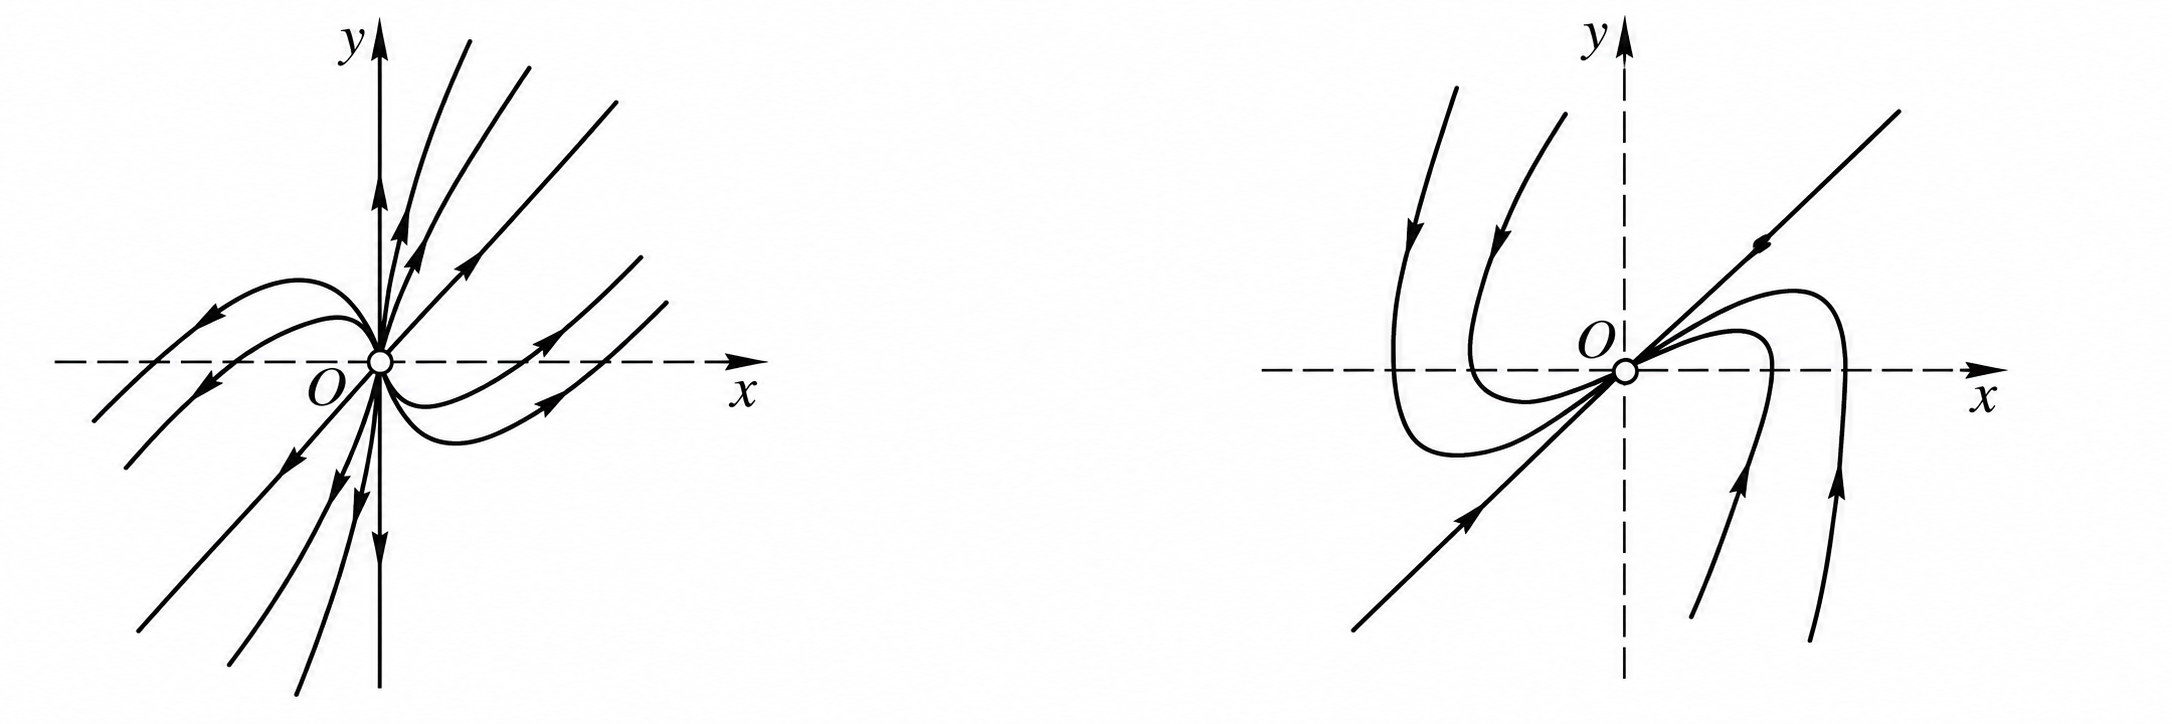
\includegraphics[width=0.7\linewidth]{figure/222}
	\label{fig:平面线性系统两例相图}
	\captionof{figure}{平面线性系统两例相图}
\end{center}


以上讨论了系数矩阵 $A$ 没有零特征根的各种情形。所有上述类型的
平衡点都称为\textbf{初等平衡点}，否则称为\textbf{退化平衡点}
（或\textbf{高阶平衡点}）。除中心以外的初等平衡点称为\textbf{粗的}，
其余平衡点称为\textbf{细的}。

下面一些内容的详细证明将在进一步关于常微分方程的学习中涉猎。
\begin{theorem}
	若非线性系统的线性部分具有粗的平衡点 $O$，则非线性系统在原点的
小邻域内与线性化系统具有相同的定性性质。
\end{theorem}
事实上，这时线性化系统的
特征根实部都不为零；即使原系统作微小改变，平衡点附近轨道的拓扑结构
仍与线性化系统相同。对于细的平衡点，非线性系统与其线性化系统未必
具有这种一致性。例如，线性部分为中心时，非线性系统的平衡点也可能
是焦点，这类情形需要进一步作中心焦点判定。

最后考虑退化平衡点，即 $\det A=0$。线性系统的特征方程为
\[
	\lambda^2-(a+d)\lambda=0,
\]
故特征根为
\[
	\lambda_1=0,
	\qquad
	\lambda_2=a+d.
\]
当 $a\neq0$ 或 $b\neq0$ 时，系统可写成
\[
	\dfrac{\dd x}{\dd t}=ax+by,
	\qquad
	\dfrac{\dd y}{\dd t}=k(ax+by),
\]
其中 $k$ 为常数。直线 $ax+by=0$ 上的所有点都是平衡点，称为
\textbf{奇线}。相空间中的轨道满足
\[
	\dfrac{\dd y}{\dd x}=k,
\]
因而是一族平行直线
\[
	y=kx+C_0.
\]
另一方面，沿轨道有
\[
	\dfrac{\dd}{\dd t}(ax+by)=\lambda_2(ax+by),
\]
从而
\[
	ax+by=C_1e^{\lambda_2t}.
\]
因此，当 $\lambda_2<0$ 时轨道趋近奇线上的点；当 $\lambda_2>0$ 时
轨道远离奇线上的点，相图见图 \ref{fig:非孤立退化平衡点相图}。
\newpage
\begin{center}
	\begin{tikzpicture}[>=Stealth,x=1cm,y=1cm]
		% a+d<0：轨道从两侧趋向奇线
		\begin{scope}[shift={(-3.45,0)}]
			\begin{scope}
				\clip (-2.5,-1.75) rectangle (2.5,2.05);
				\foreach \c in {-1.4,-.7,0,.7,1.4}{
					\pgfmathsetmacro{\ix}{\c/1.47}
					\pgfmathsetmacro{\iy}{.75*\ix}
					\draw[gray!75]
						plot[domain=-2.7:2.7,samples=2]
						(\x,{-.72*\x+\c});
					\draw[->]
						({\ix-1.05},{\iy+.756}) --
						({\ix-.13},{\iy+.0936});
					\draw[->]
						({\ix+1.05},{\iy-.756}) --
						({\ix+.13},{\iy-.0936});
					\fill[white] (\ix,\iy) circle (2.2pt);
					\draw (\ix,\iy) circle (2.2pt);
				}
				\draw[thick] (-2.35,-1.7625) -- (2.35,1.7625);
			\end{scope}
			\draw[->] (-2.55,0)--(2.55,0) node[right] {$x$};
			\draw[->] (0,-1.8)--(0,2.1) node[above] {$y$};
			\node[fill=white,inner sep=1pt,anchor=west]
				at (.72,.72) {$ax+by=0$};
			\node[below left] at (0,0) {$O$};
			\node at (0,-2.18) {$a^2+b^2\neq0$ 且 $a+d<0$};
		\end{scope}

		% a+d>0：轨道从奇线向两侧离开
		\begin{scope}[shift={(3.45,0)}]
			\begin{scope}
				\clip (-2.5,-1.75) rectangle (2.5,2.05);
				\foreach \c in {-1.4,-.7,0,.7,1.4}{
					\pgfmathsetmacro{\ix}{\c/1.47}
					\pgfmathsetmacro{\iy}{.75*\ix}
					\draw[gray!75]
						plot[domain=-2.7:2.7,samples=2]
						(\x,{-.72*\x+\c});
					\draw[->]
						({\ix-.13},{\iy+.0936}) --
						({\ix-1.05},{\iy+.756});
					\draw[->]
						({\ix+.13},{\iy-.0936}) --
						({\ix+1.05},{\iy-.756});
					\fill[white] (\ix,\iy) circle (2.2pt);
					\draw (\ix,\iy) circle (2.2pt);
				}
				\draw[thick] (-2.35,-1.7625) -- (2.35,1.7625);
			\end{scope}
			\draw[->] (-2.55,0)--(2.55,0) node[right] {$x$};
			\draw[->] (0,-1.8)--(0,2.1) node[above] {$y$};
			\node[fill=white,inner sep=1pt,anchor=west]
				at (.72,.72) {$ax+by=0$};
			\node[below left] at (0,0) {$O$};
			\node at (0,-2.18) {$a^2+b^2\neq0$ 且 $a+d>0$};
		\end{scope}
	\end{tikzpicture}
	\captionof{figure}{奇线附近轨道的趋近与远离}
	\label{fig:非孤立退化平衡点相图}
\end{center}

若 $\lambda_2=0$，则 $A$ 的两个特征根都为零，并且
$a+kb=0$。系统的通解为
\[
	x(t)=bC_0t+C_2,
	\qquad
	y(t)=dC_0t+(kC_2+C_0),
\]
其中 $C_0,C_2$ 为任意常数。此时轨道仍与奇线平行，轨道的走向由
$b,d,C_0$ 的符号确定，奇线将相平面分成的两部分中，轨道走向相反。
图 \ref{fig:双零特征根退化平衡点相图} 给出了 $b<0$、$d<0$
且 $a+d=0$ 时的相图。

\begin{center}
	\begin{tikzpicture}[>=Stealth,x=1cm,y=1cm]
		\begin{scope}
			\clip (-2.55,-2.05) rectangle (2.55,2.25);

			% 与奇线平行的轨道族
			\foreach \c in {-1.4,-.7,0,.7,1.4}{
				\draw[gray!75]
					plot[domain=-2.8:2.8,samples=2]
					(\x,{.78*\x+\c});
			}

			% 奇线上方的轨道向左下方运动
			\foreach \c in {.7,1.4}{
				\draw[->]
					(1.15,{.78*1.15+\c}) --
					(.20,{.78*.20+\c});
			}

			% 奇线下方的轨道向右上方运动
			\foreach \c in {-.7,-1.4}{
				\draw[->]
					(-1.15,{.78*(-1.15)+\c}) --
					(-.20,{.78*(-.20)+\c});
			}

			% 奇线由平衡点组成
			\draw[thick] (-2.45,-1.911) -- (2.45,1.911);
			\foreach \x in {-.72,0,.72}{
				\fill[white] (\x,{.78*\x}) circle (2.2pt);
				\draw (\x,{.78*\x}) circle (2.2pt);
			}
		\end{scope}

		\draw[dashed,->] (-2.65,0)--(2.65,0) node[right] {$x$};
		\draw[dashed,->] (0,-2.1)--(0,2.3) node[above] {$y$};
		\node[fill=white,inner sep=1pt,rotate=38]
			at (.95,.94) {$ax+by=0$};
		\node[below right] at (0,0) {$O$};
		\node at (0,-2.45) {$b<0,\ d<0$ 且 $a+d=0$};
	\end{tikzpicture}
	\captionof{figure}{双零特征根情形下奇线附近的轨道}
	\label{fig:双零特征根退化平衡点相图}
\end{center}

若 $a=b=0$，但 $c,d$ 不全为零，则 $cx+dy=0$ 为奇线，轨道是一族
平行于 $y$ 轴的直线。当 $d<0$ 时轨道趋近奇线，当 $d>0$ 时轨道
远离奇线，相图见图 \ref{fig:a等于b等于零退化平衡点相图}。
若 $a=b=c=d=0$，则平衡点充满整个相平面。

\begin{center}
	\begin{tikzpicture}[>=Stealth,x=1cm,y=1cm]
		% d<0：竖直轨道趋向奇线
		\begin{scope}[shift={(-3.35,0)}]
			\begin{scope}
				\clip (-2.35,-2.05) rectangle (2.35,2.2);
				\foreach \x in {-1.5,-.75,0,.75,1.5}{
					\pgfmathsetmacro{\iy}{.72*\x}
					\draw[gray!75] (\x,-2.2)--(\x,2.3);
					\draw[->] (\x,{\iy+1.18})--(\x,{\iy+.14});
					\draw[->] (\x,{\iy-1.18})--(\x,{\iy-.14});
					\fill[white] (\x,\iy) circle (2.2pt);
					\draw (\x,\iy) circle (2.2pt);
				}
				\draw[thick] (-2.35,-1.692)--(2.35,1.692);
			\end{scope}
			\draw[dashed,->] (-2.45,0)--(2.45,0) node[right] {$x$};
			\draw[dashed,->] (0,-2.1)--(0,2.3) node[above] {$y$};
			\node[fill=white,inner sep=1pt,anchor=west]
				at (.72,.72) {$cx+dy=0$};
			\node[below right] at (0,0) {$O$};
			\node at (0,-2.4) {$a=b=0$ 且 $d<0$};
		\end{scope}

		% d>0：竖直轨道远离奇线
		\begin{scope}[shift={(3.35,0)}]
			\begin{scope}
				\clip (-2.35,-2.05) rectangle (2.35,2.2);
				\foreach \x in {-1.5,-.75,0,.75,1.5}{
					\pgfmathsetmacro{\iy}{.72*\x}
					\draw[gray!75] (\x,-2.2)--(\x,2.3);
					\draw[->] (\x,{\iy+.14})--(\x,{\iy+1.18});
					\draw[->] (\x,{\iy-.14})--(\x,{\iy-1.18});
					\fill[white] (\x,\iy) circle (2.2pt);
					\draw (\x,\iy) circle (2.2pt);
				}
				\draw[thick] (-2.35,-1.692)--(2.35,1.692);
			\end{scope}
			\draw[dashed,->] (-2.45,0)--(2.45,0) node[right] {$x$};
			\draw[dashed,->] (0,-2.1)--(0,2.3) node[above] {$y$};
			\node[fill=white,inner sep=1pt,anchor=west]
				at (.72,.72) {$cx+dy=0$};
			\node[below right] at (0,0) {$O$};
			\node at (0,-2.4) {$a=b=0$ 且 $d>0$};
		\end{scope}
	\end{tikzpicture}
	\captionof{figure}{$a=b=0$ 时奇线附近的轨道}
	\label{fig:a等于b等于零退化平衡点相图}
\end{center}

\section{周期轨道与 Poincar\'e 映射}\label{sec:周期轨道与Poincare映射}

一个孤立的闭轨称为\textbf{极限环}。这里所谓孤立，是指在它的充分小邻域内不存在其他闭轨。极限环必为其他轨道的极限集合。

设 $\Gamma$ 是一个极限环，则在 $\Gamma$ 的内、外两侧均可取充分小的邻域，使其中不再含有其他闭轨。这些邻域内的轨道或者趋于 $\Gamma$，或者离开 $\Gamma$。由此可将极限环分为以下三类。

\begin{definition}[极限环的稳定性]
	\label{def:极限环的稳定性}
	设 $\Gamma$ 是极限环。
	\begin{enumerate}
		\item 当 $t\to+\infty$ 时，$\Gamma$ 内、外两侧的轨道都螺旋地趋于 $\Gamma$，则称 $\Gamma$ 为\textbf{稳定极限环}；
		\item 当 $t\to-\infty$ 时，$\Gamma$ 内、外两侧的轨道都螺旋地趋于 $\Gamma$，则称 $\Gamma$ 为\textbf{不稳定极限环}；
		\item 若 $\Gamma$ 一侧的轨道在 $t\to+\infty$ 时趋于 $\Gamma$，而另一侧的轨道在 $t\to-\infty$ 时趋于 $\Gamma$，则称 $\Gamma$ 为\textbf{半稳定极限环}。
	\end{enumerate}
\end{definition}

\begin{center}
	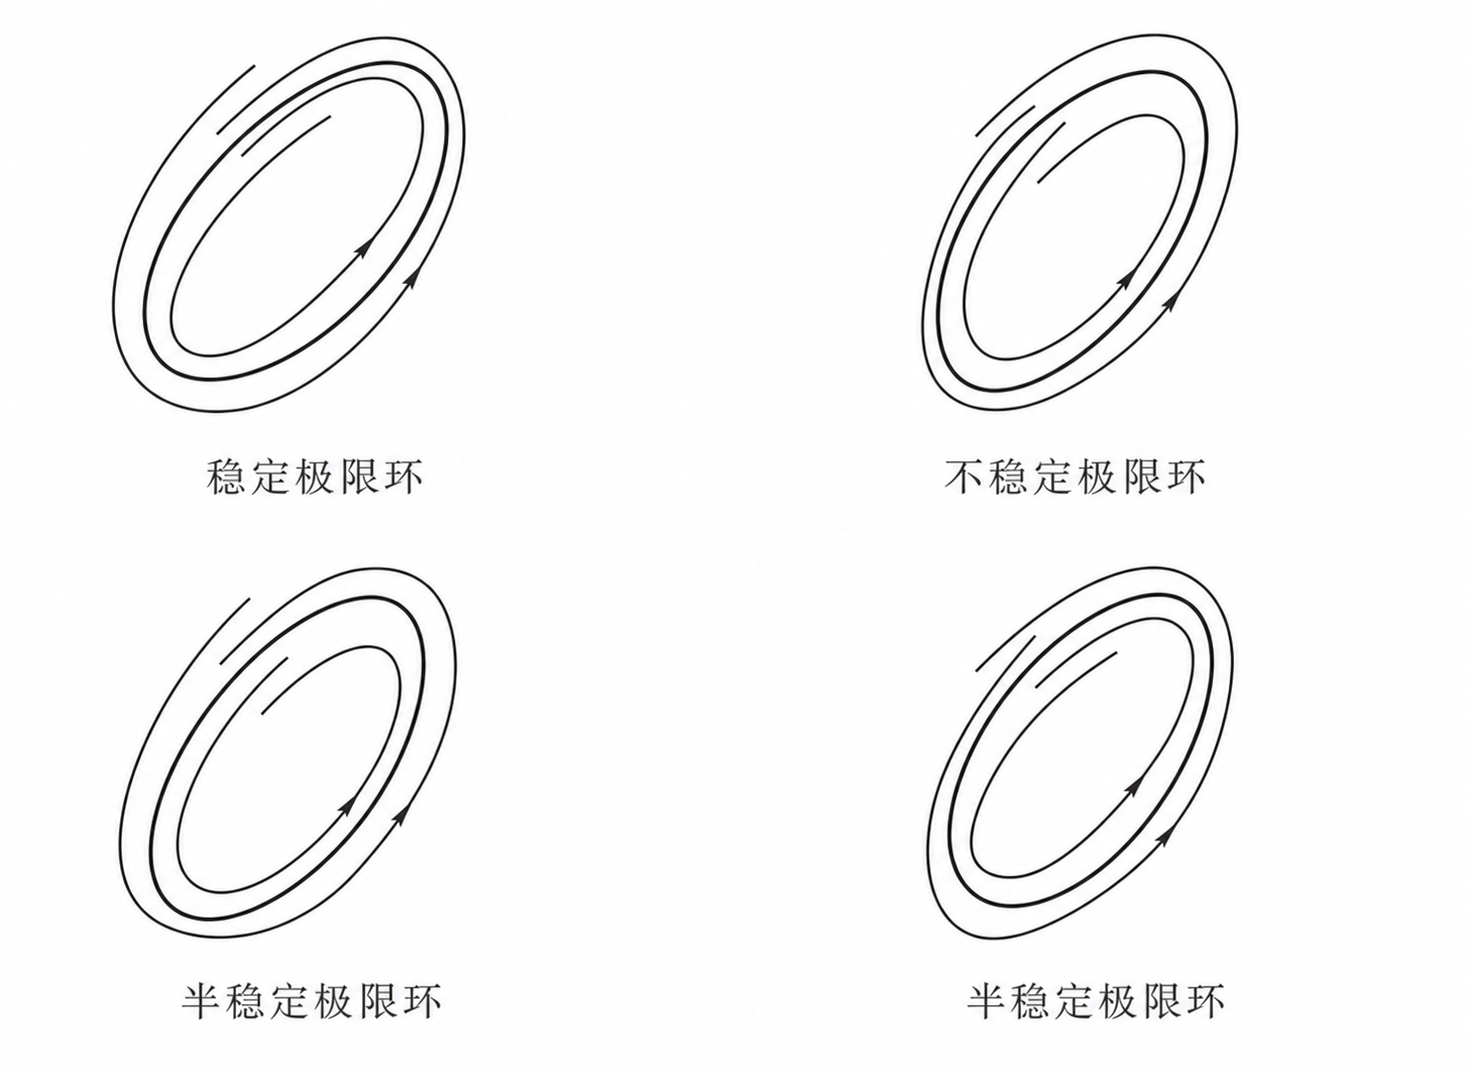
\includegraphics[width=0.6\linewidth]{figure/4}
\end{center}

\subsection*{轨道吸引与按时间参数的稳定}
\phantomsection\label{sec:orbital-versus-time}
前面的 Lyapunov 稳定性比较同一时刻的两个状态；极限环的稳定性则比较轨道与整个闭曲线的距离。为避免把两者混用，作如下区分。
\begin{definition}
周期轨道 $\Gamma$ 的轨道稳定性，是附近解始终与集合 $\Gamma$ 保持接近；
轨道吸引性是其到 $\Gamma$ 的距离趋于零。
一个指定解 $x_*(t)$ 的 Lyapunov 稳定性则比较同一时刻的
$|x(t)-x_*(t)|$，不允许任意重新选择相位。
\end{definition}
\begin{proposition}
自治系统的非常值周期解作为指定的时间函数不可能渐近稳定。
轨道渐近稳定也不一定蕴含所指定的周期解按相同时间参数比较时 Lyapunov 稳定。
\end{proposition}
\begin{proof}
任取小时间平移 $\tau$，$x_*(t+\tau)$ 也是解且初值任意接近原初值。
若相位差不是周期，连续周期函数
$|x_*(t+\tau)-x_*(t)|$ 不恒为零，也不能趋于零，故不能渐近稳定。

对第二个断言，在圆周附近使用坐标 $(u,\theta)$，其中 $u=r-1$，取
$\dot u=-u^3,\ \dot\theta=1+u$。
$u(t)=u_0/\sqrt{1+2u_0^2t}$ 始终保持小且趋于零，所以 $u=0$ 的周期轨道轨道渐近稳定。
但 $u_0>0$ 时，与 $u=0$ 解的角差为
\[
 \displaystyle\int_0^tu(s)\,\dd s=(\sqrt{1+2u_0^2t}-1)/u_0,
\]
它无界，必达到 $\pi$。届时两点相距接近圆的直径，
无论初值 $u_0$ 多小均如此，故指定的周期解不是 Lyapunov 稳定的。
\end{proof}

平衡点和闭轨都可以成为轨道的极限状态。为了更准确地描述这一现象，给出如下定义。

\begin{definition}[$\omega$ 极限集合与 $\alpha$ 极限集合]
	\label{def:极限集合}
	设自治系统过 $\vect x_0$ 的轨道为 $\vect x=\vect \varphi(t,\vect x_0)$。若存在序列 $t_n\to+\infty$，使
	\[
		\vect \varphi(t_n,x_0)\to \vect x^*,
	\]
	则称 $\vect x^*$ 为轨道的一个 $\omega$ 极限点；所有 $\omega$ 极限点组成的集合称为 $\omega$ 极限集合，记为 $\omega(\vect x_0,\vect \varphi)$。类似地，以 $t_n\to-\infty$ 定义 $\alpha$ 极限点和 $\alpha$ 极限集合 $\alpha(\vect x_0,\vect \varphi)$。轨道的极限集合定义为
	\[
		L(\vect x_0,\vect \varphi):=\omega(\vect x_0,\vect \varphi)\cup\alpha(\vect x_0,\vect \varphi).
	\]
\end{definition}

若一条轨道是平衡点或闭轨，则它的 $\omega$ 极限集合和 $\alpha$ 极限集合都是轨道本身。由于 Jordan 曲线定理\footnote{也就是平面上任一简单闭曲线$\gamma$把平面分割为两部分，连接这两部分中任意点的连续路径必与$\gamma$相交。}，平面自治系统的极限集合具有较为简单的结构。

\begin{theorem}(Poincar\'e--Bendixson 环域定理)
	\label{thm:PoincareBendixson环域定理}
	设 $X(x,y),Y(x,y)$ 在区域 $G$ 内连续可微，$\overline D$ 是 $G$ 内的有界环形闭区域，并且
	\[
		\overline D=L_1\cup D\cup L_2,
	\]
	其中 $L_1$、$L_2$ 分别是 $\overline D$ 的内、外边界，均为简单闭曲线且都不是闭轨。若 $\overline D$ 内没有平衡点，并且从 $L_1$、$L_2$ 出发的轨道或者都不能离开 $\overline D$，或者都不能进入 $\overline D$，则 $D$ 内至少存在一条闭轨 $\Gamma$。
\end{theorem}

\begin{center}
	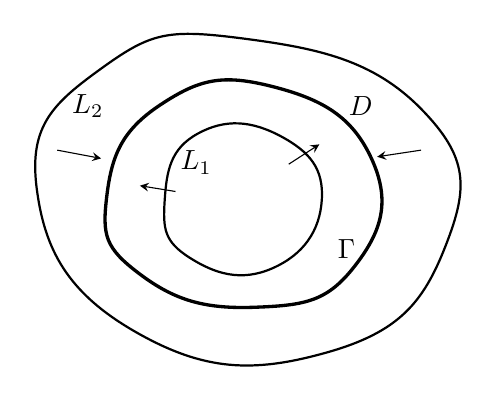
\begin{tikzpicture}[>=stealth,scale=1.05]
		\draw[thick] plot[smooth cycle,tension=.85] coordinates {(-2.4,.2) (-1.6,1.65) (.1,2) (2.25,1.15) (2.55,-.5) (1.1,-1.8) (-1.2,-1.55)};
		\draw[thick] plot[smooth cycle,tension=.85] coordinates {(-.85,.05) (-.45,.85) (.55,.82) (1.05,.05) (.45,-.78) (-.55,-.65)};
		\draw[very thick] plot[smooth cycle,tension=.85] coordinates {(-1.55,.1) (-.9,1.2) (.45,1.42) (1.65,.55) (1.45,-.75) (.25,-1.25) (-1.15,-.85)};
		\node at (-1.78,1.18) {$L_2$};
		\node at (-.47,.50) {$L_1$};
		\node at (1.52,1.18) {$D$};
		\node at (1.35,-.55) {$\Gamma$};
		\draw[->] (-2.15,.65)--(-1.62,.55);
		\draw[->] (2.25,.65)--(1.72,.57);
		\draw[->] (-.72,.15)--(-1.15,.22);
		\draw[->] (.65,.48)--(1.02,.72);
	\end{tikzpicture}
	\captionof{figure}{Poincar\'e--Bendixson 环域定理中的环形区域}
	\label{fig:PoincareBendixson环域}
\end{center}

在图~\ref{fig:PoincareBendixson环域} 中，$L_1$、$L_2$ 分别为环形区域的内、外边界。利用定理~\ref{thm:PoincareBendixson环域定理}，不仅可以证明闭轨的存在性，还可以通过选取较窄的环形区域来估计闭轨所在的位置。

\paragraph{例 6.6}
考虑系统
\[
	\begin{cases}
		x'=y+x(1-x^2-y^2),\\
		y'=-x+y(1-x^2-y^2).
	\end{cases}
\]
该系统只有一个平衡点 $O$。取
\[
	L_1:x^2+y^2=r_1^2<1,\qquad
	L_2:x^2+y^2=r_2^2>1,
\]
并以 $L_1,L_2$ 为内、外边界构成环形区域 $D$。令
\[
	V(x,y)=x^2+y^2,
\]
则沿系统的轨道有
\[
	\begin{aligned}
		\dfrac{\mathrm dV}{\mathrm dt}
		&=2x\bigl[y+x(1-x^2-y^2)\bigr]
		 +2y\bigl[-x+y(1-x^2-y^2)\bigr]\\
		&=2(x^2+y^2)(1-x^2-y^2).
	\end{aligned}
\]
因此，在 $L_1$ 上 $\dfrac{\mathrm dV}{\mathrm dt}>0$，在 $L_2$ 上 $\dfrac{\mathrm dV}{\mathrm dt}<0$，两条边界上的轨道都进入 $D$。由 Poincar\'e--Bendixson 环域定理，$D$ 内存在闭轨。

作极坐标变换
\[
	x=r\cos\theta,\qquad y=r\sin\theta,
\]
可得
\[
	\dfrac{\mathrm dr}{\mathrm dt}=r(1-r^2),\qquad
	\dfrac{\mathrm d\theta}{\mathrm dt}=-1.
\]
其解为
\[
	r(t)=\dfrac{1}{\sqrt{1+Ce^{-2t}}},\qquad
	\theta(t)=-(t-t_0),
\]
即
\[
	x(t)=\dfrac{\cos(t-t_0)}{\sqrt{1+Ce^{-2t}}},\qquad
	y(t)=\dfrac{-\sin(t-t_0)}{\sqrt{1+Ce^{-2t}}}.
\]
当 $C=0$ 时，得到闭轨
\[
	\Gamma:x^2+y^2=1.
\]
当 $C>0$ 时，轨道从 $\Gamma$ 内侧螺旋地趋于 $\Gamma$；当 $C<0$ 时，轨道从 $\Gamma$ 外侧螺旋地趋于 $\Gamma$。因此，$\Gamma$ 是系统唯一的稳定极限环，其相图如图~\ref{fig:示例稳定极限环相图} 所示。

\begin{center}
	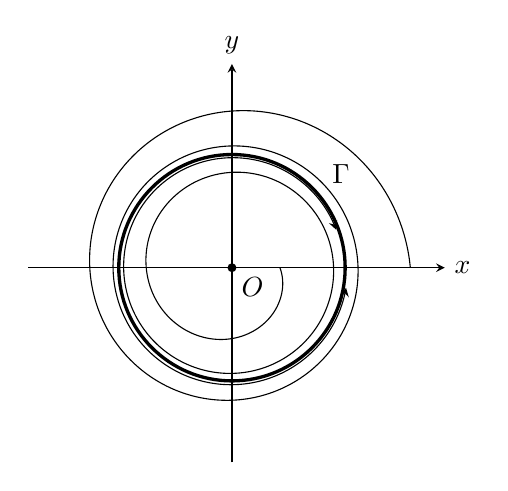
\begin{tikzpicture}[>=stealth,scale=1.15]
		\draw[->] (-2.25,0)--(2.35,0) node[right] {$x$};
		\draw[->] (0,-2.15)--(0,2.25) node[above] {$y$};
		\draw[very thick] (0,0) circle (1.25);
		\draw[->,domain=0:710,samples=260,smooth,variable=\t]
			plot ({(1.25+.72*exp(-.0045*\t))*cos(\t)},
			      {(1.25+.72*exp(-.0045*\t))*sin(\t)});
		\draw[->,domain=0:700,samples=260,smooth,variable=\t]
			plot ({(1.25-.72*exp(-.0048*\t))*cos(-\t)},
			      {(1.25-.72*exp(-.0048*\t))*sin(-\t)});
		\fill (0,0) circle (1.4pt) node[below right] {$O$};
		\node[above right] at (1.0,.82) {$\Gamma$};
	\end{tikzpicture}
	\captionof{figure}{例 6.6 的相图}
	\label{fig:示例稳定极限环相图}
\end{center}

下面给出两个判定平面自治系统不存在闭轨的准则。

\begin{theorem}[Bendixson 判据]
	\label{thm:Bendixson判据}
	设 $X(x,y),Y(x,y)$ 在区域 $G$ 内连续可微。若在单连通区域 $D\subset G$ 内，函数
	\[
		\dfrac{\partial X}{\partial x}+\dfrac{\partial Y}{\partial y}
	\]
	不变号，并且在 $D$ 的任何子区域内不恒等于零，则系统在 $D$ 内不存在闭轨。
\end{theorem}

\begin{proof}
	反设 $D$ 内存在闭轨 $\Gamma$，其参数方程为
	\[
		x=x(t),\qquad y=y(t),\qquad 0\leqslant t\leqslant T,
	\]
	并以 $D_0$ 表示 $\Gamma$ 所围成的区域。由 Green 公式，
	\[
		\begin{aligned}
			\iint_{D_0}\left(
			\dfrac{\partial X}{\partial x}
			+\dfrac{\partial Y}{\partial y}\right)\mathrm dx\mathrm dy
			&=\oint_{\Gamma}X\,\mathrm dy-Y\,\mathrm dx\\
			&=\int_0^T\left(X\dfrac{\mathrm dy}{\mathrm dt}
			-Y\dfrac{\mathrm dx}{\mathrm dt}\right)\mathrm dt=0.
		\end{aligned}
	\]
	但由假设，上述二重积分不可能为零，矛盾。
\end{proof}

\begin{theorem}[Dulac 判据]
	\label{thm:Dulac判据}
	设 $X(x,y),Y(x,y)$ 在区域 $G$ 内连续可微。若在单连通区域 $D\subset G$ 内存在连续可微函数 $B(x,y)$，使
	\[
		\dfrac{\partial(BX)}{\partial x}
		+\dfrac{\partial(BY)}{\partial y}
	\]
	不变号，并且在 $D$ 的任何子区域内不恒等于零，则系统在 $D$ 内不存在闭轨。函数 $B(x,y)$ 称为\textbf{Dulac 函数}。
\end{theorem}

寻找 Dulac 函数同寻找 Lyapunov 函数一样，需要一定的技巧。

\begin{proof}
	若 $D$ 内存在闭轨 $\Gamma$，设其围成区域为 $D_0$。由 Green 公式及 $\dot x=X,\dot y=Y$，有
	\[
		\begin{aligned}
			\iint_{D_0}\left[
			\dfrac{\partial(BX)}{\partial x}
			+\dfrac{\partial(BY)}{\partial y}\right]\mathrm dx\mathrm dy
			&=\oint_{\Gamma}BX\,\mathrm dy-BY\,\mathrm dx\\
			&=\int_0^T B(x(t),y(t))
			\left(X\dfrac{\mathrm dy}{\mathrm dt}
			-Y\dfrac{\mathrm dx}{\mathrm dt}\right)\mathrm dt=0.
		\end{aligned}
	\]
	这与被积函数不变号且在任何子区域内不恒为零矛盾。
\end{proof}

下面介绍后继函数。设原点 $O$ 是系统的中心型平衡点，即其线性化系统的平衡点为中心。为判别非线性系统的原点究竟是中心还是焦点，并研究原点附近闭轨的个数，需要考察相邻轨道在一条横截线上的交点。

在 $O$ 的充分小邻域 $B_\delta$ 内，非线性系统等价于本章前面给出的标准形式，其中非线性项充分小。取正 $x$ 轴为 $\Sigma$，令 $\Sigma_0=\Sigma\cap B_\delta$，并任取 $P_0\in\Sigma_0$。线性系统从 $P_0$ 出发的轨道经过一周后回到 $P_0$。由解对初值的连续依赖性，非线性系统从 $P_0$ 出发的轨道经过一周后与 $\Sigma_0$ 交于 $P_1$，且 $P_1$ 接近 $P_0$。于是可以定义映射
\[
	\Pi:\Sigma_0\longrightarrow\Sigma,\qquad
	\Pi(P_0)=P_1.
\]

\begin{definition}[Poincar\'e 映射]
	\label{def:Poincare映射}
	上述 $\Sigma_0$ 称为系统的一个\textbf{Poincar\'e 截面}，或称\textbf{横截线}；映射 $\Pi$ 称为\textbf{Poincar\'e 映射}。函数
	\[
		d(P):=\Pi(P)-P
	\]
	称为\textbf{后继函数}。
\end{definition}

原点附近的闭轨与 $\Pi$ 的不动点一一对应，即
\[
	\Pi(Q)=Q,\qquad Q\in\Sigma_0.
\]
若 $Q$ 是 $\Pi$ 的吸引不动点或排斥不动点，则后继函数在 $Q$ 两侧具有相应的符号变化，而与 $Q$ 对应的闭轨分别为稳定极限环或不稳定极限环。

\begin{center}
	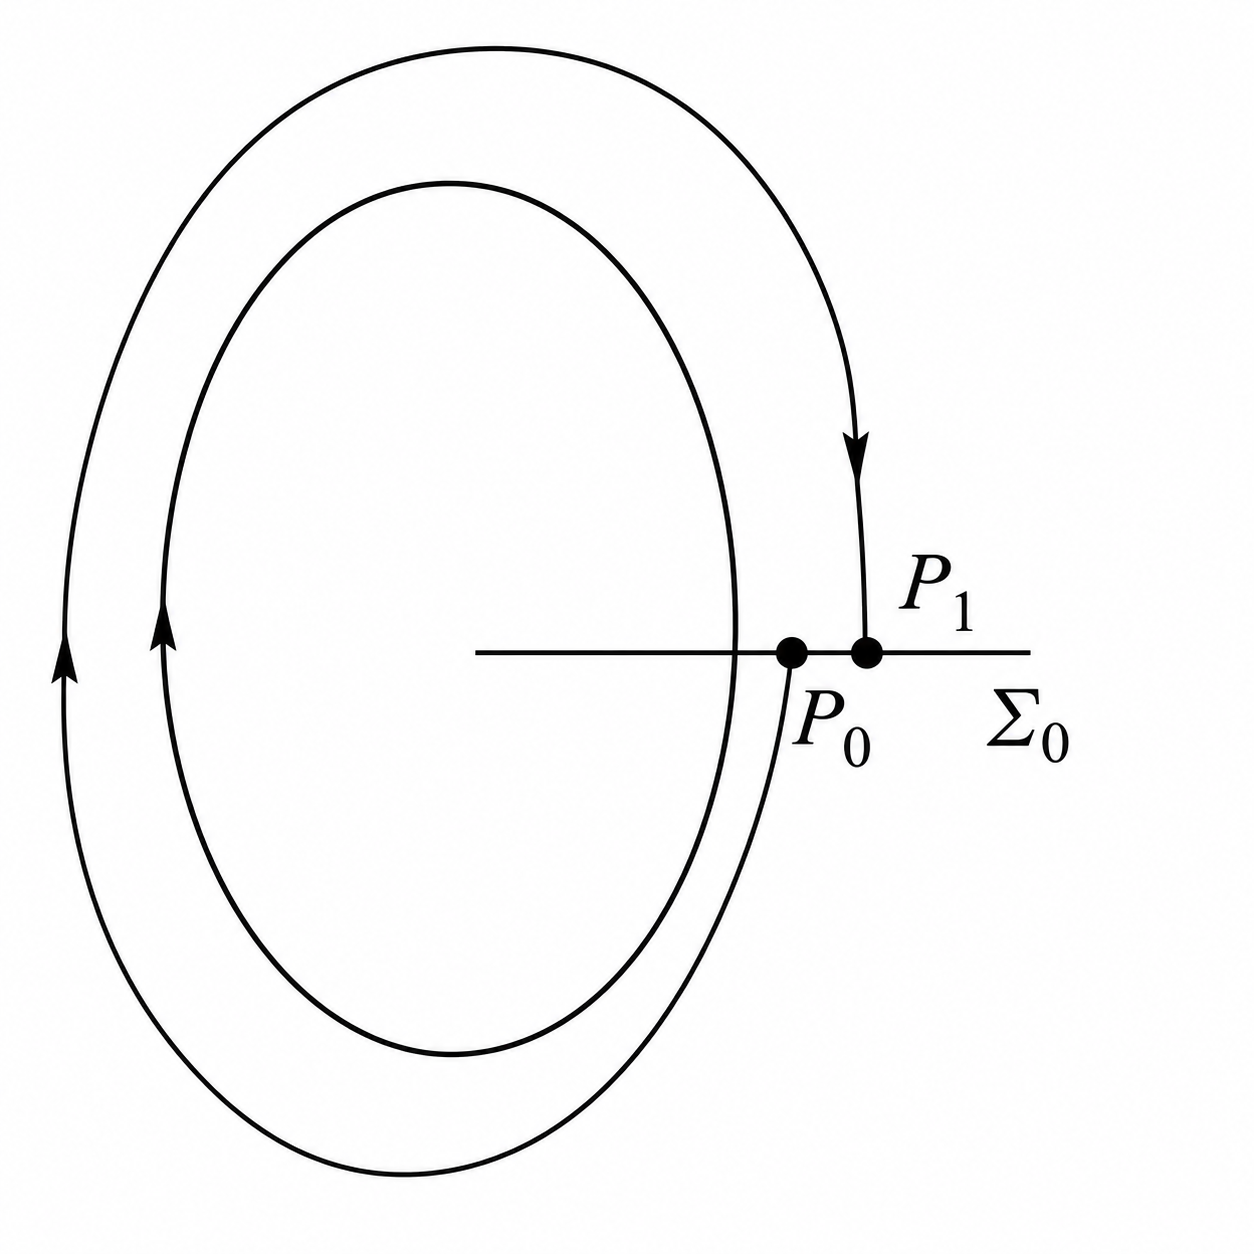
\includegraphics[width=0.5\linewidth]{figure/5}
	
	\captionof{figure}{Poincar\'e 映射与后继函数}
	\label{fig:Poincare映射}
\end{center}

Poincar\'e 映射把连续的轨道运动化为映射的迭代，因此将连续动力系统与离散动力系统联系起来。

\begin{definition}[离散动力系统]
	\label{def:离散动力系统}
	设 $X\subset\mathbb R^n$，$f:X\to X$ 是连续自映射。令
	\[
		f^0(x)=x,\qquad
		f^k(x)=f\bigl(f^{k-1}(x)\bigr),\quad k=2,3,\ldots.
	\]
	则半群
	\[
		\{f^k:k=0,1,2,\ldots\}
	\]
	称为由 $f$ 生成的离散半动力系统。若 $f$ 是同胚，则还可以考虑群
	\[
		\{f^k:k=0,\pm1,\pm2,\ldots\}.
	\]
	这就是离散动力系统。
\end{definition}

连续过程可以通过取样离散化，离散过程也可以嵌入连续过程之中。对于同胚 $f:X\to X$，定义
\[
	\begin{aligned}
		\operatorname{Orb}_f(x_0)
		&=\{f^k(x_0):k=0,\pm1,\pm2,\ldots\},\\
		\operatorname{Orb}_f^+(x_0)
		&=\{f^k(x_0):k=0,1,2,\ldots\},\\
		\operatorname{Orb}_f^-(x_0)
		&=\{f^{-k}(x_0):k=0,1,2,\ldots\}.
	\end{aligned}
\]
它们分别称为 $x_0$ 的轨道、正半轨道和负半轨道。

若存在自然数 $p$，使 $f^p(x_0)=x_0$，则称 $x_0$ 为 $f$ 的\textbf{周期点}；使该等式成立的最小自然数 $p$ 称为 $x_0$ 的\textbf{周期}。也就是说，
\[
	f^p(x_0)=x_0,\qquad
	f^k(x_0)\ne x_0,\quad k=1,2,\ldots,p-1.
\]
周期为 $1$ 的点称为不动点。$f$ 的周期点集合与不动点集合分别记为 $\operatorname{Per}(f)$ 和 $\operatorname{Fix}(f)$。

\begin{proposition}[一维周期点的导数判据]\label{prop:discrete-derivative-test}
对于一维区间上的连续映射 $f:I\to I$，若 $x_0$ 是周期为 $p$ 的周期点，且 $f^p$ 在 $x_0$ 处可微，则当
\[
	\left|(f^p)'(x_0)\right|<1
\]
时，$x_0$ 是稳定周期点；当
\[
	\left|(f^p)'(x_0)\right|>1
\]
时，$x_0$ 是不稳定周期点。类似的有稳定不动点与不稳定不动点。
\end{proposition}
\begin{proof}
令 $g=f^p$，则 $g(x_0)=x_0$。若 $|g'(x_0)|<1$，取 $|g'(x_0)|<q<1$。
由导数的定义，充分靠近 $x_0$ 时，
\[
 |g(x)-x_0|\leq q|x-x_0|.
\]
这个小邻域被 $g$ 映入自身，归纳得到 $|g^n(x)-x_0|\leq q^n|x-x_0|$，故每隔 $p$ 步的迭代稳定且趋于 $x_0$。
再对有限多个连续映射 $f^j$（$0\leq j<p$）使用连续性，就同时控制了周期内其余各步，得到周期轨道的稳定性与吸引性。

若 $|g'(x_0)|>1$，取 $1<q<|g'(x_0)|$。同样由导数的定义，在某个固定小邻域内有
\[
 |g(x)-x_0|\geq q|x-x_0|.
\]
任一非零初始偏差若始终留在该邻域，就会在迭代后至少增大为原来的 $q^n$ 倍，产生矛盾。
因此无论初始偏差多小，均有一次迭代离开这个固定邻域，故周期点不稳定。
\end{proof}


\subsection*{返回映射与保守振动的小扰动}
\phantomsection\label{sec:perturbed-oscillation}
闭轨与 Poincar\'e 映射的不动点相对应。下面利用解经过一周后的能量差求出不动点，并应用命题~\ref{prop:discrete-derivative-test} 判断稳定性。返回时间的存在性由第五章的可微依赖性与隐函数定理保证。考虑下列振动方程及其小扰动
\[
 \dot x=y+\varepsilon f(x,y,\varepsilon),\qquad
 \dot y=-x+\varepsilon g(x,y,\varepsilon),
\]
假定 $f,g$ 足够光滑。未扰动能量为 $E=(x^2+y^2)/2$。
\begin{definition}
系统在没有外部周期强迫的条件下自行形成稳定的周期运动，称为自激振动。
稳定周期运动的振幅由方程确定。下面利用横截面上的返回映射研究这种周期运动。
\end{definition}
\begin{theorem}[一周能量增量]
固定 $A_0>0$，在其附近以 $A$ 为初始半径，从正 $x$ 轴作一周返回。
设返回能量与初始能量之差为 $\Delta E(A,\varepsilon)$。则
\[
 \Delta E(A,\varepsilon)=\varepsilon M(A)+O(\varepsilon^2),\qquad
 M(A)=\int_0^{2\pi}(xf+yg)(A\cos t,-A\sin t,0)\,\dd t.
\]
若 $M(A_0)=0$、$M'(A_0)\ne0$，则充分小非零 $\varepsilon$ 时存在邻近的唯一周期轨道。
当 $\varepsilon M'(A_0)<0$ 时它横向渐近稳定，符号相反时不稳定。
\end{theorem}
\begin{proof}
在半径 $A_0$ 附近取一个不含原点的小闭环带。未扰动解为
$(A\cos t,-A\sin t)$，在 $t=2\pi$ 横截正 $x$ 轴，因为此时
$\dot y=-A\ne0$。将横截条件写为 $y(t,A,\varepsilon)=0$，
在 $(2\pi,A_0,0)$ 对 $t$ 的导数非零。解的光滑依赖和隐函数定理给出光滑返回时间
$\tau(A,\varepsilon)$，且 $\tau(A,0)=2\pi$。
在该闭环带中角速度保持为负，故这一交点确是转过一周后的首次返回。
缩小参数邻域后，统一有
\[
 \tau(A,\varepsilon)=2\pi+O(\varepsilon),\qquad
 (x(t),y(t))=(A\cos t,-A\sin t)+O(\varepsilon)
\]
于所需的有界时间段内成立。

令 $B(x,y,\varepsilon)=xf(x,y,\varepsilon)+yg(x,y,\varepsilon)$。
沿解直接求导，线性项抵消，得到 $\dot E=\varepsilon B$。因此
\[
 \Delta E=\varepsilon\int_0^{\tau(A,\varepsilon)}B(x(t),y(t),\varepsilon)\,dt.
\]
被积函数在紧环带上有界且具有有界的一阶导数。改变轨道和参数使积分改变
$O(\varepsilon)$，将上限改为 $2\pi$ 又只改变 $O(\varepsilon)$；
乘外面的 $\varepsilon$ 后即得 $\Delta E=\varepsilon M(A)+O(\varepsilon^2)$。
同样估计可对 $A$ 求导，因而余项在 $C^1$ 意义下也成立。

为在 $\varepsilon=0$ 使用隐函数定理，定义
\[
 D(A,\varepsilon)=\int_0^1\partial_\varepsilon
 \Delta E(A,s\varepsilon)\,ds.
\]
微积分基本定理给出 $\Delta E=\varepsilon D$，且 $D(A,0)=M(A)$。
因 $\partial_AD(A_0,0)=M'(A_0)\ne0$，方程 $D=0$ 有唯一邻近解 $A(\varepsilon)$。
正 $x$ 轴上 $E=A^2/2$ 严格递增，故能量返回原值恰等价于返回同一点。
存在唯一性随即保证这条解为周期解；局部唯一性指横截面交点邻近 $A_0$ 的闭轨。

设半径返回映射为 $P_\varepsilon$。对
$[P_\varepsilon(A)^2-A^2]/2=\varepsilon D(A,\varepsilon)$ 求导，
再在 $P_\varepsilon(A)=A=A(\varepsilon)$ 处取值，得
\[
 P_\varepsilon'(A(\varepsilon))
 =1+\frac{\varepsilon}{A(\varepsilon)}\partial_AD(A(\varepsilon),\varepsilon)
 =1+\frac{\varepsilon M'(A_0)}{A_0}+O(\varepsilon^2).
\]
当 $\varepsilon M'(A_0)<0$ 且参数充分小时，该导数模小于 1，
横截面上的不动点渐近稳定，周期内部由流的连续依赖控制，故闭轨横向渐近稳定。
符号相反时导数大于 1，不动点及闭轨均横向不稳定。
\end{proof}
\begin{example}[Van der Pol 振动]
对 $\ddot x=-x+\varepsilon\dot x(1-x^2)$，取 $f=0,g=y(1-x^2)$。
于是
\[
 M(A)=\int_0^{2\pi}A^2\sin^2t(1-A^2\cos^2t)\,\dd t
 =\pi A^2-\frac\pi4A^4.
\]
$M(2)=0$、$M'(2)=-4\pi$，所以 $\varepsilon>0$ 充分小时有振幅接近 2 的稳定极限环。
上述存在性与唯一性结论只在半径 2 附近成立，并以参数充分小为条件。
\end{example}


图~\ref{fig:ode-tikz-return-map} 示意横截面上的半径如何逐次趋近闭轨；这对应返回映射在不动点处的压缩。
\begin{center}
\begin{minipage}{0.96\linewidth}
\centering
% TikZ mathematical illustration; compiled with the main document.
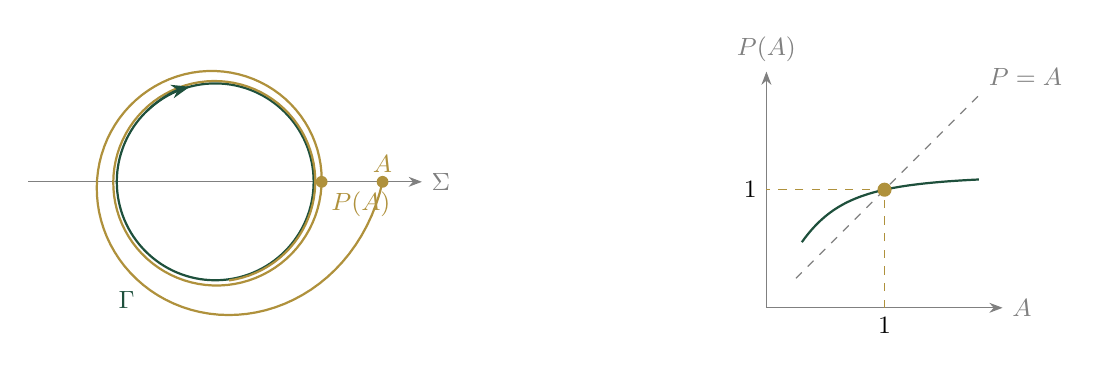
\begin{tikzpicture}[>=Stealth,font=\small]
\begin{scope}[scale=1.25]
 \draw[gray,->] (-1.9,0)--(2.1,0) node[right]{$\Sigma$};
 \draw[GreenMain,thick] (0,0) circle(1);
 \draw[GoldMain,thick,domain=0:14,samples=200,variable=\t]
  plot ({cos(\t r)/sqrt(1+(1/2.89-1)*exp(-.24*\t))},{-sin(\t r)/sqrt(1+(1/2.89-1)*exp(-.24*\t))});
 \draw[->,GreenMain,thick] (135:1) arc[start angle=135,end angle=105,radius=1];
 \fill[GoldMain] (1.7,0) circle(1.7pt) node[above]{$A$};
 \fill[GoldMain] ({1/sqrt(1+(1/2.89-1)*exp(-.24*2*pi))},0) circle(1.7pt) node[below right]{$P(A)$};
 \node[GreenMain] at (-.9,-1.2){$\Gamma$};
\end{scope}
\begin{scope}[shift={(7,-1.6)},scale=1.5]
 \draw[->,gray] (0,0)--(2,0) node[right]{$A$};
 \draw[->,gray] (0,0)--(0,2) node[above]{$P(A)$};
 \draw[gray,dashed] (.25,.25)--(1.8,1.8) node[above right]{$P=A$};
 \draw[GreenMain,thick,domain=.3:1.8,samples=70] plot (\x,{1/sqrt(1+(1/(\x*\x)-1)*exp(-.24*2*pi))});
 \draw[GoldMain,dashed] (1,0)--(1,1)--(0,1);
 \fill[GoldMain] (1,1) circle(1.7pt);
 \node[below] at (1,0){$1$};\node[left] at (0,1){$1$};
\end{scope}
\end{tikzpicture}
\captionof{figure}{返回映射的吸引不动点与吸引闭轨：模型 $\dot r=0.12r(1-r^2)$、$\dot\theta=-1$。}
\label{fig:ode-tikz-return-map}
\end{minipage}
\end{center}

\subsection*{一般区间映射的周期行为}
下面讨论一般区间映射的周期点。这些映射不一定是微分方程的返回映射。

\paragraph{例 6.8}
考虑 Logistic 映射
\[
	f_\lambda:I=[0,1]\longrightarrow I,\qquad
	f_\lambda(x)=\lambda x(1-x),\qquad \lambda\in[0,4].
\]
它有不动点
\[
	x_1=0,\qquad x_2=1-\dfrac{1}{\lambda}.
\]
当 $\lambda<1$ 时，只有不动点 $x_1$，并且它是稳定的；当 $1<\lambda<3$ 时，$x_1$ 变为不稳定不动点，同时产生稳定不动点 $x_2$；当 $\lambda>3$ 时，$x_2$ 变为不稳定不动点，并产生两个周期为 $2$ 的周期点
\[
	x_{\pm}=\dfrac{1}{2\lambda}
	\left(1+\lambda\pm\sqrt{(\lambda+1)(\lambda-3)}\right).
\]
它们由方程 $f_\lambda^2(x)=x$ 得到。当
\[
	3<\lambda<1+\sqrt6
\]
时，这两个周期点是稳定的。随着参数 $\lambda$ 继续增大，稳定周期轨道的周期依次由
\[
	1\longrightarrow2\longrightarrow4\longrightarrow8\longrightarrow\cdots
\]
不断加倍，这种现象称为\textbf{倍周期分岔}，也称为\textbf{Feigenbaum 分岔}。参数值
\[
	\lambda=1,\quad3,\quad1+\sqrt6,\quad\ldots
\]
称为分岔点。其分岔图见图~\ref{fig:Feigenbaum分岔现象}。

\begin{center}
	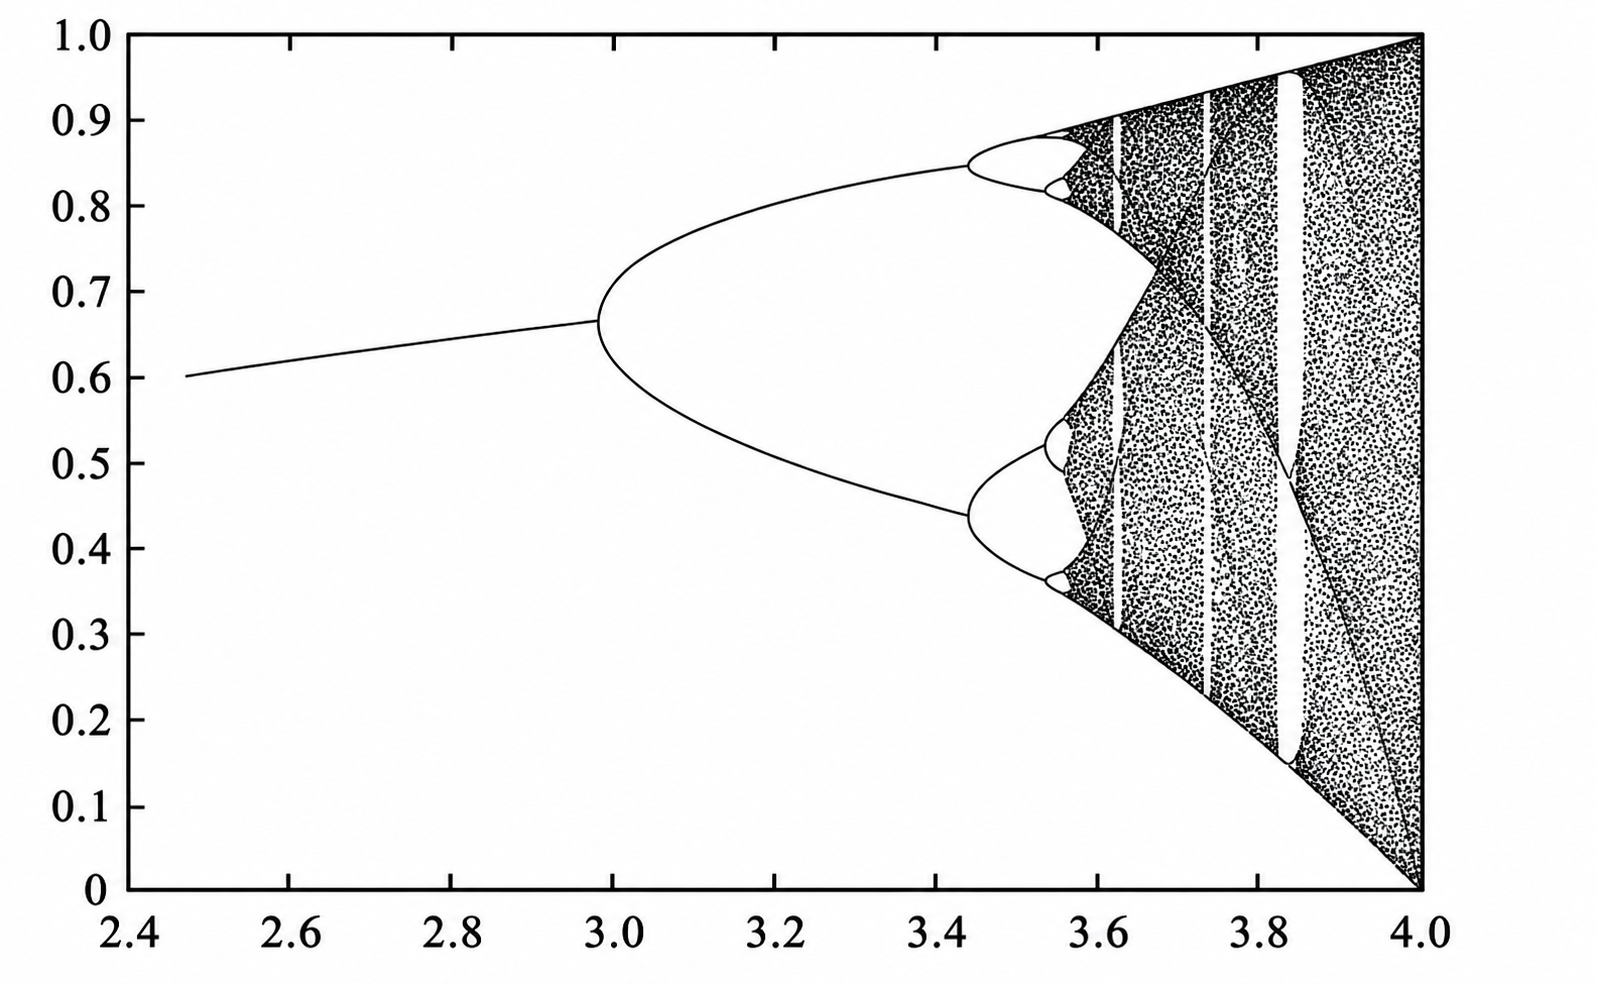
\includegraphics[width=0.7\linewidth]{figure/3}
	
	\captionof{figure}{Feigenbaum 分岔现象}
	\label{fig:Feigenbaum分岔现象}
\end{center}

1964年，Sharkovsky对自然数做了重新排序，对于闭区间上的连续自映射，其周期之间存在如下 Sharkovsky 次序：
\[
\begin{aligned}
	3&\triangleleft5\triangleleft7\triangleleft\cdots
	\triangleleft(2n+1)\triangleleft(2n+3)\triangleleft\cdots\\
	&\triangleleft2\cdot3\triangleleft2\cdot5\triangleleft2\cdot7\triangleleft\cdots\\
	&\triangleleft2^2\cdot3\triangleleft2^2\cdot5\triangleleft2^2\cdot7\triangleleft\cdots\\
	&\qquad\vdots\\
	&\triangleleft2^m\cdot3\triangleleft2^m\cdot5\triangleleft2^m\cdot7\triangleleft\cdots\\
	&\qquad\vdots\\
	&\triangleleft2^\ell\triangleleft2^{\ell-1}\triangleleft\cdots
	\triangleleft16\triangleleft8\triangleleft4\triangleleft2\triangleleft1.
\end{aligned}
\]
并证明了以下重要的结果，它全面揭示了一维迭代动力系统的周期性规律。
\begin{theorem}(Sharkovsky 定理)
	\label{thm:Sharkovsky定理}
	设 $I\subset\mathbb R$ 是闭区间，$f:I\to I$ 是连续自映射。若 $f$ 有周期为 $p$ 的周期点，则对每个自然数 $m$，只要
	\[
		p\triangleleft m,
	\]
	$f$ 就有周期为 $m$ 的周期点。
\end{theorem}

\section{平面 Hamilton 系统}\label{sec:平面Hamilton系统}

在这一节中，我们应用前面的定性理论方法来分析一类在物理学中重要的系统，即 Hamilton 系统。

\begin{definition}\label{def:Hamilton系统}
	令 $W\subset\mathbb R^{2n}$ 为开集，$\vect x,\vect y\in\mathbb R^n$，且 $(\vect x,\vect y)\in W$，$H(\vect x,\vect y)$ 为定义在 $W$ 上的连续可微实函数。称系统
	\[
		\dfrac{\dd \vect x}{\dd t}=\dfrac{\partial H}{\partial \vect y},
		\qquad
		\dfrac{\dd \vect y}{\dd t}=-\dfrac{\partial H}{\partial \vect x}
	\]
	为 $W$ 上带 $n$ 个自由度的 \textbf{Hamilton 系统}，称 $H(\vect x,\vect y)$ 为该系统的 \textbf{Hamilton 函数}。其中
	\[
	\begin{aligned}
		\vect x&=(x_1,x_2,\ldots,x_n)^{\mathrm T},
		&\vect y&=(y_1,y_2,\ldots,y_n)^{\mathrm T},\\
		\dfrac{\partial H}{\partial \vect x}
		&=\left(
		\dfrac{\partial H}{\partial x_1},
		\dfrac{\partial H}{\partial x_2},\ldots,
		\dfrac{\partial H}{\partial x_n}
		\right)^{\mathrm T},
		&
		\dfrac{\partial H}{\partial \vect y}
		&=\left(
		\dfrac{\partial H}{\partial y_1},
		\dfrac{\partial H}{\partial y_2},\ldots,
		\dfrac{\partial H}{\partial y_n}
		\right)^{\mathrm T}.
	\end{aligned}
	\]
\end{definition}

在经典天体力学的多体问题和无阻尼的机械振动中，常常会遇到 Hamilton 系统。这时 Hamilton 函数 $H(x,y)$ 往往表示相应力学系统的总能量，因此一般又称它为能量函数。下面给出 Hamilton 函数的一个重要性质。

\begin{theorem}(Hamilton 函数的守恒性)\label{thm:Hamilton函数沿轨道守恒}
	Hamilton 系统的 Hamilton 函数 $H(x,y)$ 沿该系统的轨道等于常数。
\end{theorem}

\begin{proof}
	设 $(x(t),y(t))$ 为 Hamilton 系统的解，则 $H(x(t),y(t))$ 是 $t$ 的函数，并且
	\[
	\begin{aligned}
		\dfrac{\dd}{\dd t}H(x(t),y(t))
		&=\dfrac{\partial H}{\partial x}\dfrac{\dd x}{\dd t}
		 +\dfrac{\partial H}{\partial y}\dfrac{\dd y}{\dd t}\\
		&=\dfrac{\partial H}{\partial x}\dfrac{\partial H}{\partial y}
		 -\dfrac{\partial H}{\partial y}\dfrac{\partial H}{\partial x}=0.
	\end{aligned}
	\]
	故沿着轨道 $(x(t),y(t))$，函数 $H(x,y)$ 为常数。
\end{proof}

\begin{corollary}[Hamilton相流保持体积]\label{cor:hamilton-volume}
若 Hamilton 函数 $H$ 属于 $C^2$，则 Hamilton 相流保持相空间体积。
\end{corollary}
\begin{proof}
对 Hamilton 场 $v=(H_p,-H_q)$，逐坐标计算得
\[
 \operatorname{div}v
 =\sum_i\left(\frac{\partial^2H}{\partial q_i\partial p_i}
 -\frac{\partial^2H}{\partial p_i\partial q_i}\right)=0.
\]
最后一步使用 $H\in C^2$ 时混合偏导相等，因而散度恒为零。

再应用定理~\ref{thm:nonlinear-liouville} 即得结论。
\end{proof}

上述定理表明，在无阻尼的机械振动系统中，系统的总能量保持不变，即 Hamilton 系统满足能量等值定律。一般把满足能量等值定律的系统称为保守系统，因此 Hamilton 系统是保守系统。

带一个自由度的 Hamilton 系统称为\textbf{平面 Hamilton 系统}。前面许多例子都涉及如下形式的微分方程：
\[
	\dfrac{\dd^2x}{\dd t^2}+g(x)=0,
\]
其中 $x\in\mathbb R$，$g(x)$ 为 $\mathbb R$ 上的连续可微函数。若用 $y$ 表示速度，则该方程等价于
\[
	\dfrac{\dd x}{\dd t}=y,
	\qquad
	\dfrac{\dd y}{\dd t}=-g(x).
\]
这是一个 Hamilton 系统，其 Hamilton 函数为
\[
	H(x,y)=\dfrac{y^2}{2}+G(x),
\]
其中
\[
	G(x)=\int_0^x g(s)\,\dd s.
\]
$G(x)$ 是系统运动的势能，$\dfrac{y^2}{2}$ 是系统运动的动能，因此这类特殊的平面 Hamilton 系统也称为“动能 $+$ 势能”型 Hamilton 系统。

容易看出，$(x_0,y_0)$ 为上述系统的平衡点，当且仅当
\[
	y_0=0,\qquad g(x_0)=0.
\]
在这种情形下 $G'(x_0)=0$，因此 $x_0$ 为势能函数 $G(x)$ 的临界点。

\begin{theorem}(平衡点的分类)\label{thm:动能加势能型Hamilton系统平衡点分类}
	上述系统的平衡点都在 $x$ 轴上，$(x_0,0)$ 为平衡点当且仅当 $G'(x_0)=0$。
若这一临界点非退化，即 $G''(x_0)\ne0$，则 $G''(x_0)<0$ 时 $(x_0,0)$ 为鞍点，$G''(x_0)>0$ 时为中心。
仅有“严格极值”而不附加非退化条件时，不能将它与二阶导数严格有符号写成等价条件。
\end{theorem}

\begin{proof}
	先设 $G'(x_0)=0$ 且 $G''(x_0)<0$，即 $x_0$ 为非退化的严格极大值点。此时
	\[
		G'(x_0)=g(x_0)=0,
		\qquad
		G''(x_0)=g'(x_0)<0.
	\]
	在 $(x_0,0)$ 处，系统右端函数的 Jacobi 矩阵为
	\[
		A=\begin{pmatrix}
			0&1\\
			-g'(x_0)&0
		\end{pmatrix}.
	\]
	此时
	\[
		\operatorname{tr}A=0,
		\qquad
		\det A=g'(x_0)<0,
	\]
	故矩阵 $A$ 有两个符号相反的非零实特征根，因而 $(x_0,0)$ 为系统的鞍点。

	再设 $G'(x_0)=0$ 且 $G''(x_0)>0$，即 $x_0$ 为非退化的严格极小值点。此时
	\[
		G'(x_0)=g(x_0)=0,
		\qquad
		G''(x_0)=g'(x_0)>0.
	\]
	Jacobi 矩阵仍为上面的矩阵 $A$，同时
	\[
		\operatorname{tr}A=0,
		\qquad
		\det A=g'(x_0)>0.
	\]
	因此，矩阵 $A$ 的两个特征根是一对共轭纯虚根，故 $(x_0,0)$ 为系统线性部分的中心。

	为了进一步证明 $(x_0,0)$ 也是原系统的中心，由定理~\ref{thm:Hamilton函数沿轨道守恒}，系统在平衡点 $(x_0,0)$ 附近的轨道形成相平面中的一族曲线
	\[
		V(x,y)=\dfrac{y^2}{2}+G(x)-G(x_0)=C,
	\]
	其中 $C$ 为常数。显然 $V(x_0,0)=0$。又由于 $x_0$ 为 $G(x)$ 的严格极小值点，存在 $(x_0,0)$ 的闭邻域
	\[
		N_\delta=\left\{(x,y)\in\mathbb R^2:
		(x-x_0)^2+y^2\leqslant\delta^2\right\},
	\]
	使得在 $N_\delta\setminus\{(x_0,0)\}$ 上 $V(x,y)>0$。令
	\[
		l=\min_{(x,y)\in\partial N_\delta}V(x,y),
	\]
	其中
	\[
		\partial N_\delta=\left\{(x,y)\in\mathbb R^2:
		(x-x_0)^2+y^2=\delta^2\right\}
	\]
	是 $N_\delta$ 的边界。

	由 $G''(x_0)>0$ 及连续性，可将 $\delta$ 取得足够小，使
\[
 D^2V(x,y)=\operatorname{diag}(G''(x),1)
\]
在 $N_\delta$ 上处处正定。固定单位方向 $e$，令
$v_e(r)=V((x_0,0)+re)$。因为 $v_e(0)=v_e'(0)=0$ 且 $v_e''(r)>0$，
所以 $v_e$ 对 $0<r\leq\delta$ 严格增加。
对每个 $0<C<l$，介值定理及严格单调性给出唯一的 $r=r_C(e)\in(0,\delta)$，使 $v_e(r)=C$。
又有 $v_e'(r_C(e))>0$，故隐函数定理说明 $r_C$ 随方向光滑变化。
因此 $V=C$ 在此邻域中是一条围绕 $(x_0,0)$ 的光滑简单闭曲线，而不只是与每条径向线相交的集合。

在该曲线上 $\nabla V\ne0$，Hamilton 向量场为 $(V_y,-V_x)$，因而处处非零并与曲线相切。
紧性给出速度的正下界，而曲线弧长有限，所以解在有限时间内走完一周，确实形成周期轨道。
当 $C\downarrow0$ 时，这些互不相交的闭轨收缩到平衡点；它们覆盖一个去心邻域，故 $(x_0,0)$ 为中心。
\end{proof}
\begin{center}
	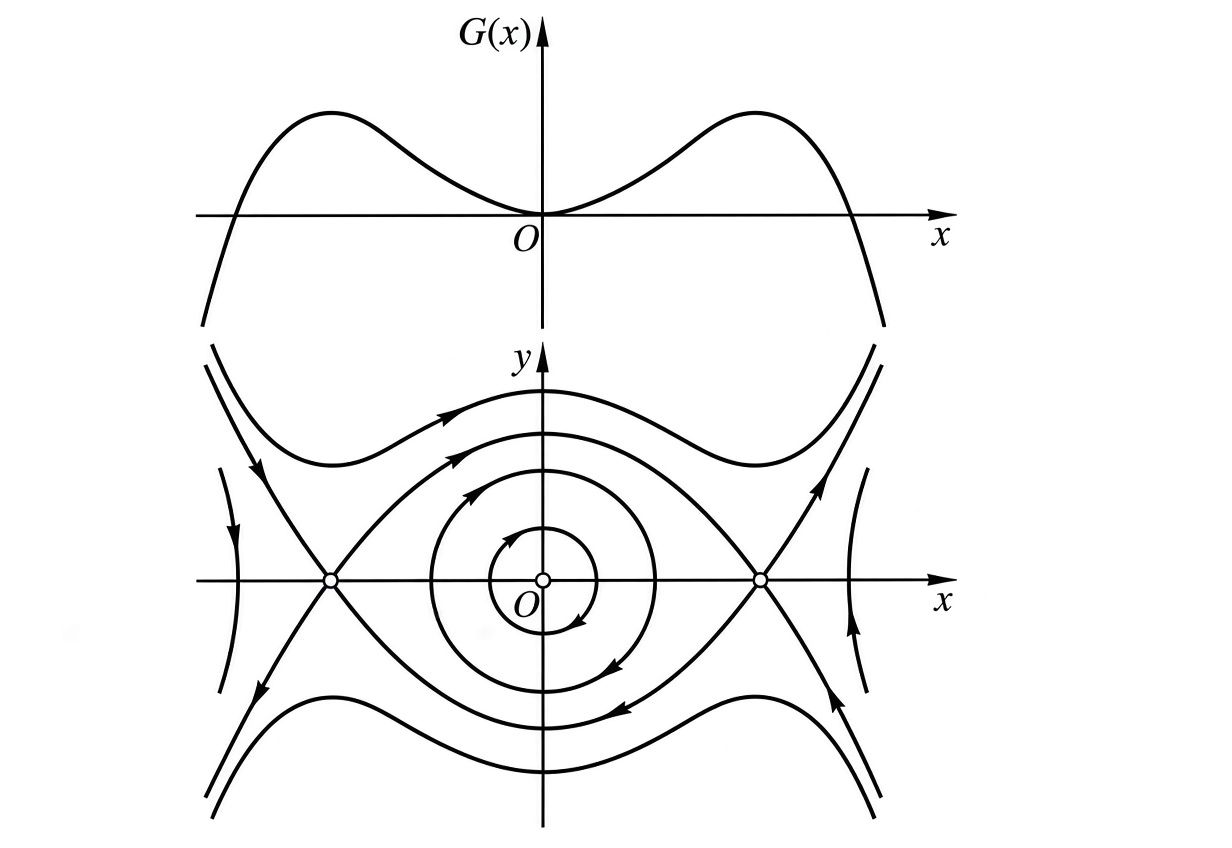
\includegraphics[width=0.7\linewidth]{figure/6}
	\captionof{figure}{系统的势能函数与相图}
	\label{fig:动能加势能型Hamilton系统相图}
\end{center}

由定理~\ref{thm:动能加势能型Hamilton系统平衡点分类}，如果势能函数 $G(x)$ 的临界点均非退化，就可以由 $G(x)$ 的图像在 $Oxy$ 坐标系中画出系统的相图，如图~\ref{fig:动能加势能型Hamilton系统相图} 所示。除平衡点均在 $x$ 轴上外，轨道由曲线族
\[
	H(x,y)=C
\]
给出，并且关于 $x$ 轴对称。



\subsection*{能量层的轨道分解与振动周期}
\phantomsection\label{sec:energy-levels}
由定理~\ref{thm:Hamilton函数沿轨道守恒}，每条轨道都包含在一个能量等值集中。下面讨论非临界能量等值集中的轨道，并计算闭轨的周期。解的全局延拓可用定理~\ref{thm:energy-global-extension} 判断。
\begin{definition}
对一自由度系统 $\ddot x=-U'(x)$，记能量
$H(x,y)=y^2/2+U(x)$。若 $E$ 不等于任何 $U$ 的临界值，称为非临界能量。
满足 $U(a)=E$ 的位置称为转向点；当 $U'(a)\ne0$ 时称为简单转向点。
趋近平衡点的非平衡轨道称为分离轨道；两端趋于同一平衡点时称同宿轨道，
趋于两个不同平衡点时称异宿轨道。
\end{definition}
\begin{theorem}[非临界能量层]\label{thm:regular-energy-level}
设 $U\in C^2(\R)$，$E$ 为非临界能量。
集合 $\{x:U(x)<E\}$ 的每个有界连通分支 $(a,b)$ 对应一条闭轨，周期为
\[
 T(E)=2\int_a^b\frac{\dd x}{\sqrt{2(E-U(x))}}.
\]
无界分支对应直线型轨道；当该集合为整个实轴时，对应两条轨道
$y=\pm\sqrt{2(E-U(x))}$。
\end{theorem}
\begin{proof}
设 $(a,b)$ 是 $\{U<E\}$ 的一个有界连通分支。连续性给出
$U(a)=U(b)=E$；非临界假设又给出 $U'(a),U'(b)\ne0$。
由分支内部 $U<E$，必有 $U'(a)<0$、$U'(b)>0$。一阶展开于是给出
\[
 \begin{aligned}
 \lim_{x\downarrow a}\frac{E-U(x)}{x-a}&=-U'(a)>0,\\
 \lim_{x\uparrow b}\frac{E-U(x)}{b-x}&=U'(b)>0.
\end{aligned}
\]
故存在正常数 $c_1,c_2$，使靠近左端时
\[
 c_1(x-a)\leq E-U(x)\leq c_2(x-a);
\]
右端有对应估计。
因为 $\displaystyle\int_0^\delta s^{-1/2}\,ds=2\sqrt\delta<\infty$，下式收敛：
\[
 \tau=\int_a^b\frac{dx}{\sqrt{2(E-U(x))}}.
\]
在上半支 $y=\sqrt{2(E-U(x))}$ 上，$\dot x=y>0$，分离变量说明
从 $a$ 到 $b$ 的时间正是 $\tau$。到达 $(b,0)$ 时，向量场为
$(0,-U'(b))$，竖直向下且非零；存在唯一性把解接到下半支。
下半支满足 $\dot x=-\sqrt{2(E-U(x))}$，在同样的时间 $\tau$ 内返回 $(a,0)$。
在 $(a,0)$ 处向量场竖直向上，解遂重复。第一次回到初始状态需要完整走过两支，
故其最小正周期为 $2\tau$。

再看曲线的光滑性。能量层上
$\nabla H=(U'(x),y)$ 不为零，隐函数定理表明它在每一点附近都是可用单个坐标参数化的光滑曲线。
在转向点附近可用 $y$ 为坐标，因此两条显式平方根分支虽然在 $x$ 坐标中
斜率无穷，接合后的曲线仍光滑。两支加两个端点构成一条简单闭曲线。

若分支只有一个有限端点，正负两支经此端点接合，构成一条非闭合的直线型曲线。
若分支是整个实轴，则 $y$ 始终不为零，两支分别构成两条直线型曲线。
每一支上的非零向量场使任意两个有限位置之间的行程时间有限，
所以这里所述每条连通曲线确是一条最大轨道的像。
这些分支穷尽全部非临界能量层，分类因而完整。
\end{proof}
在临界能量层，$U'(a)=0$、$y=0$ 的点本身是一条平衡轨道，
不能同与之相接的分离轨道算成一条轨道。
唯一性说明非平衡运动不可能在有限时间到达平衡点；
若它在有限端点有此极限，则延拓后与常值解具有同一初值，矛盾。


图~\ref{fig:ode-tikz-energy-level} 将转向点与相平面中的上下两支对应起来；箭头表示真实的时间方向。
\begin{center}
\begin{minipage}{0.96\linewidth}
\centering
% TikZ mathematical illustration; compiled with the main document.
\begin{tikzpicture}[>=Stealth,font=\small]
\begin{scope}[x=1.2cm,y=1.45cm]
 \draw[->,gray] (-2,0)--(2.2,0) node[right]{$x$};
 \draw[->,gray] (0,-.18)--(0,2) node[above]{$U$};
 \draw[GreenMain,thick,domain=-1.8:1.8,samples=60] plot (\x,{\x*\x/2});
 \draw[GoldMain,thick] (-1.95,1)--(1.95,1) node[right]{$E$};
 \foreach \a/\lab in {-1.4142/a,1.4142/b}{
  \draw[dashed,gray] (\a,0)--(\a,1);
  \fill[GoldMain] (\a,1) circle(1.5pt);
  \node[below] at (\a,0){$\lab$};
 }
 \node at (0,-.55){允许位置：$a\leq x\leq b$};
\end{scope}
\begin{scope}[shift={(7,1.15)},scale=1.05]
 \draw[->,gray] (-1.85,0)--(1.95,0) node[right]{$x$};
 \draw[->,gray] (0,-1.8)--(0,1.9) node[above]{$y$};
 \draw[GreenMain,thick] (0,0) circle(1.4142);
 \draw[->,GreenMain,thick] (105:1.4142) arc[start angle=105,end angle=75,radius=1.4142];
 \draw[->,GreenMain,thick] (285:1.4142) arc[start angle=285,end angle=255,radius=1.4142];
 \fill[GoldMain] (-1.4142,0) circle(1.6pt) node[below left]{$(a,0)$};
 \fill[GoldMain] (1.4142,0) circle(1.6pt) node[below right]{$(b,0)$};
 \node at (0,-2.1){$y^2/2+U(x)=E$};
\end{scope}
\end{tikzpicture}
\captionof{figure}{势阱与闭合能量层：以 $U(x)=x^2/2$、$E=1$ 为例。}
\label{fig:ode-tikz-energy-level}
\end{minipage}
\end{center}

\begin{proposition}[数学摆的周期]
对 $\ddot x=-\sin x$，振幅 $0<A<\pi$ 时
\[
 T(A)=4\int_0^{\pi/2}
 \frac{\dd u}{\sqrt{1-k^2\sin^2u}},\qquad k=\sin(A/2).
\]
当 $A\to0$，
$T(A)=2\pi(1+A^2/16+O(A^4))$；当 $A\uparrow\pi$ 时周期按对数阶发散。
\end{proposition}
\begin{proof}
能量式给出 
\[
 \dot x^2=2(\cos x-\cos A).
\]
把四分之一周期的积分中令 $\sin(x/2)=k\sin u$，约去 $\cos u$，得到上述公式。
小 $k$ 时，积分号内一致展开为
$1+\frac12k^2\sin^2u+O(k^4)$，再用
$\displaystyle\int_0^{\pi/2}\sin^2u\,\dd u=\pi/4$ 和 $k^2=A^2/4+O(A^4)$ 即得渐近式。

令 $\delta=1-k^2$。在 $u=\pi/2$ 附近写 $s=\pi/2-u$，
分母平方是 $\delta+k^2\sin^2s$。
小 $s$ 时 $\sin s$ 与 $s$ 之比有正常数上下界，所以相应积分与
$\displaystyle\int_0^c(\delta+s^2)^{-1/2}\,\dd s$ 同阶。
后一积分为 $\operatorname{arsinh}(c/\sqrt\delta)$，是 $|\log\delta|$ 阶；
离开端点的部分有界，故证明对数发散。
\end{proof}

\begin{definition}[商拓扑、圆周与圆柱]\label{def:quotient-circle}
设 $X$ 是拓扑空间，$X/{\sim}$ 是某等价关系确定的商集，$\pi:X\to X/{\sim}$ 为自然映射。规定 $U\subset X/{\sim}$ 开当且仅当 $\pi^{-1}(U)$ 开，称商拓扑。
关系 $x\sim y\Longleftrightarrow x-y\in2\pi\Z$ 给出圆周 $\R/2\pi\Z$，
映射 $[x]\mapsto(\cos x,\sin x)$ 将其与单位圆对应。
圆柱是圆周与实线的乘积：$(\R/2\pi\Z)\times\R$，其点由一个角度类及一个实数给出。
乘积拓扑以各因子开集的乘积为一组基。
\end{definition}

角度 $x$ 与 $x+2\pi$ 表示同一位置，因此摆的自然相空间是圆柱
$(\R/2\pi\Z)\times\R$。平面展开图中不闭合的旋转运动，在圆柱上可以闭合。


\subsection*{Lotka--Volterra系统的闭轨与平均值}
\phantomsection\label{sec:lv-energy}
对于绪论中的捕食者--食饵模型，也可以先求首次积分，再由其等值线判断轨道是否闭合。设 $a,b,c,d$ 为正数，考虑
\[
 \dot x=x(-a+by),\qquad \dot y=y(c-dx),\qquad x,y>0.
\]
\begin{theorem}
函数
\[
 H(x,y)=dx-c\log x+by-a\log y
\]
是首次积分。正象限内除平衡点 $(c/d,a/b)$ 外的每条轨道均闭合。
任意周期轨道上，$x,y$ 的时间平均值分别为 $c/d,a/b$。
\end{theorem}
\begin{proof}
直接相乘可得
\[
 \dot H=(dx-c)(-a+by)+(by-a)(c-dx)=0.
\]
$H$ 的 Hessian 为 $\operatorname{diag}(c/x^2,a/y^2)$，正定；
$H$ 向象限边界或无穷远均趋于无穷，所以有唯一严格最小点 $(c/d,a/b)$。
每个非最小等值集紧，且梯度非零。
从最小点沿任意射线出发，$H$ 严格增加到无穷，因此每个较高等值集
在每个方向上恰交一点，并由隐函数定理构成一条光滑简单闭曲线。
向量场在其上非零且相切，紧性给出非零速度的正下界，所以有限时间内走完一周。

设周期为 $T$。对 $\dot x/x=-a+by$ 积分得
\[
 0=-aT+b\displaystyle\int_0^Ty(t)\,\dd t,
\]
对 $\dot y/y$ 积分得
\[
 0=cT-d\displaystyle\int_0^Tx(t)\,\dd t.
\]
除以 $T$ 即得平均值。
\end{proof}


图~\ref{fig:ode-tikz-lv-levels} 中闭轨围绕唯一极小点，各坐标的周期平均值均为 1。
\begin{center}
\begin{minipage}{0.96\linewidth}
\centering
% TikZ mathematical illustration; compiled with the main document.
\begin{tikzpicture}[>=Stealth,font=\small,x=1.8cm,y=1.55cm]
 \draw[->,gray] (0,0)--(3,0) node[right]{$x$};
 \draw[->,gray] (0,0)--(0,3) node[above]{$y$};
 \draw[dashed,GoldMain] (1,0)--(1,2.85);
 \draw[dashed,GoldMain] (0,1)--(2.85,1);
\draw[GreenMain,thick] plot coordinates {(1.45502,1.00000) (1.45462,1.01588) (1.45344,1.03171) (1.45152,1.04746) (1.44888,1.06309) (1.44557,1.07857) (1.44162,1.09387) (1.43706,1.10897) (1.43194,1.12386) (1.42628,1.13851) (1.42012,1.15291) (1.41349,1.16706) (1.40641,1.18095) (1.39891,1.19456) (1.39102,1.20791) (1.38274,1.22098) (1.37411,1.23377) (1.36514,1.24629) (1.35583,1.25852) (1.34620,1.27048) (1.33626,1.28216) (1.32603,1.29355) (1.31549,1.30467) (1.30467,1.31549) (1.29355,1.32603) (1.28216,1.33626) (1.27048,1.34620) (1.25852,1.35583) (1.24629,1.36514) (1.23377,1.37411) (1.22098,1.38274) (1.20791,1.39102) (1.19456,1.39891) (1.18095,1.40641) (1.16706,1.41349) (1.15291,1.42012) (1.13851,1.42628) (1.12386,1.43194) (1.10897,1.43706) (1.09387,1.44162) (1.07857,1.44557) (1.06309,1.44888) (1.04746,1.45152) (1.03171,1.45344) (1.01588,1.45462) (1.00000,1.45502) (0.98412,1.45461) (0.96830,1.45338) (0.95257,1.45129) (0.93699,1.44836) (0.92161,1.44457) (0.90649,1.43993) (0.89168,1.43446) (0.87722,1.42819) (0.86316,1.42115) (0.84954,1.41339) (0.83639,1.40495) (0.82374,1.39589) (0.81160,1.38627) (0.80000,1.37614) (0.78894,1.36556) (0.77842,1.35459) (0.76845,1.34329) (0.75900,1.33171) (0.75007,1.31989) (0.74165,1.30788) (0.73373,1.29573) (0.72627,1.28345) (0.71928,1.27109) (0.71272,1.25867) (0.70658,1.24621) (0.70085,1.23372) (0.69549,1.22124) (0.69051,1.20876) (0.68587,1.19629) (0.68158,1.18384) (0.67760,1.17142) (0.67394,1.15903) (0.67058,1.14667) (0.66751,1.13434) (0.66472,1.12203) (0.66221,1.10976) (0.65996,1.09750) (0.65798,1.08527) (0.65627,1.07306) (0.65481,1.06087) (0.65361,1.04868) (0.65268,1.03651) (0.65200,1.02433) (0.65160,1.01217) (0.65146,1.00000) (0.65160,0.98783) (0.65202,0.97567) (0.65274,0.96350) (0.65376,0.95134) (0.65509,0.93918) (0.65675,0.92704) (0.65875,0.91492) (0.66110,0.90282) (0.66383,0.89077) (0.66693,0.87877) (0.67044,0.86685) (0.67436,0.85502) (0.67872,0.84330) (0.68352,0.83172) (0.68877,0.82031) (0.69449,0.80910) (0.70069,0.79811) (0.70736,0.78738) (0.71451,0.77695) (0.72213,0.76684) (0.73021,0.75708) (0.73874,0.74771) (0.74771,0.73874) (0.75708,0.73021) (0.76684,0.72213) (0.77695,0.71451) (0.78738,0.70736) (0.79811,0.70069) (0.80910,0.69449) (0.82031,0.68877) (0.83172,0.68352) (0.84330,0.67872) (0.85502,0.67436) (0.86685,0.67044) (0.87877,0.66693) (0.89077,0.66383) (0.90282,0.66110) (0.91492,0.65875) (0.92704,0.65675) (0.93918,0.65509) (0.95134,0.65376) (0.96350,0.65274) (0.97567,0.65202) (0.98783,0.65160) (1.00000,0.65146) (1.01217,0.65160) (1.02433,0.65200) (1.03651,0.65268) (1.04868,0.65361) (1.06087,0.65481) (1.07306,0.65627) (1.08527,0.65798) (1.09750,0.65996) (1.10976,0.66221) (1.12203,0.66472) (1.13434,0.66751) (1.14667,0.67058) (1.15903,0.67394) (1.17142,0.67760) (1.18384,0.68158) (1.19629,0.68587) (1.20876,0.69051) (1.22124,0.69549) (1.23372,0.70085) (1.24621,0.70658) (1.25867,0.71272) (1.27109,0.71928) (1.28345,0.72627) (1.29573,0.73373) (1.30788,0.74165) (1.31989,0.75007) (1.33171,0.75900) (1.34329,0.76845) (1.35459,0.77842) (1.36556,0.78894) (1.37614,0.80000) (1.38627,0.81160) (1.39589,0.82374) (1.40495,0.83639) (1.41339,0.84954) (1.42115,0.86316) (1.42819,0.87722) (1.43446,0.89168) (1.43993,0.90649) (1.44457,0.92161) (1.44836,0.93699) (1.45129,0.95257) (1.45338,0.96830) (1.45461,0.98412) (1.45502,1.00000)};
\draw[->,GreenMain,thick] (1.28216,1.33626)--(1.38002,1.25069);
\draw[->,GreenMain,thick] (0.65481,1.06087)--(0.66888,1.19010);
\draw[->,GreenMain,thick] (1.12203,0.66472)--(0.99495,0.63732);
\draw[GreenMain,thick] plot coordinates {(1.98625,1.00000) (1.98508,1.03440) (1.98170,1.06865) (1.97629,1.10261) (1.96903,1.13619) (1.96010,1.16929) (1.94967,1.20186) (1.93789,1.23384) (1.92490,1.26521) (1.91083,1.29595) (1.89579,1.32604) (1.87988,1.35549) (1.86317,1.38431) (1.84574,1.41250) (1.82765,1.44007) (1.80895,1.46705) (1.78967,1.49344) (1.76986,1.51928) (1.74952,1.54456) (1.72869,1.56931) (1.70737,1.59355) (1.68556,1.61728) (1.66329,1.64053) (1.64053,1.66329) (1.61728,1.68556) (1.59355,1.70737) (1.56931,1.72869) (1.54456,1.74952) (1.51928,1.76986) (1.49344,1.78967) (1.46705,1.80895) (1.44007,1.82765) (1.41250,1.84574) (1.38431,1.86317) (1.35549,1.87988) (1.32604,1.89579) (1.29595,1.91083) (1.26521,1.92490) (1.23384,1.93789) (1.20186,1.94967) (1.16929,1.96010) (1.13619,1.96903) (1.10261,1.97629) (1.06865,1.98170) (1.03440,1.98508) (1.00000,1.98625) (0.96560,1.98503) (0.93138,1.98127) (0.89754,1.97486) (0.86428,1.96572) (0.83181,1.95383) (0.80036,1.93924) (0.77010,1.92207) (0.74122,1.90248) (0.71384,1.88071) (0.68806,1.85705) (0.66394,1.83179) (0.64148,1.80524) (0.62069,1.77771) (0.60149,1.74949) (0.58383,1.72083) (0.56761,1.69196) (0.55275,1.66307) (0.53915,1.63431) (0.52670,1.60580) (0.51531,1.57763) (0.50489,1.54987) (0.49536,1.52257) (0.48663,1.49575) (0.47864,1.46943) (0.47132,1.44361) (0.46461,1.41829) (0.45847,1.39345) (0.45284,1.36907) (0.44768,1.34513) (0.44296,1.32161) (0.43864,1.29848) (0.43471,1.27571) (0.43112,1.25328) (0.42788,1.23115) (0.42494,1.20930) (0.42232,1.18770) (0.41998,1.16632) (0.41792,1.14513) (0.41613,1.12410) (0.41462,1.10322) (0.41337,1.08244) (0.41240,1.06176) (0.41169,1.04114) (0.41126,1.02056) (0.41111,1.00000) (0.41126,0.97944) (0.41172,0.95886) (0.41251,0.93825) (0.41364,0.91759) (0.41514,0.89687) (0.41703,0.87609) (0.41936,0.85523) (0.42215,0.83431) (0.42546,0.81332) (0.42931,0.79229) (0.43378,0.77123) (0.43890,0.75018) (0.44475,0.72919) (0.45139,0.70830) (0.45888,0.68758) (0.46729,0.66712) (0.47667,0.64701) (0.48709,0.62735) (0.49857,0.60824) (0.51116,0.58981) (0.52484,0.57216) (0.53960,0.55539) (0.55539,0.53960) (0.57216,0.52484) (0.58981,0.51116) (0.60824,0.49857) (0.62735,0.48709) (0.64701,0.47667) (0.66712,0.46729) (0.68758,0.45888) (0.70830,0.45139) (0.72919,0.44475) (0.75018,0.43890) (0.77123,0.43378) (0.79229,0.42931) (0.81332,0.42546) (0.83431,0.42215) (0.85523,0.41936) (0.87609,0.41703) (0.89687,0.41514) (0.91759,0.41364) (0.93825,0.41251) (0.95886,0.41172) (0.97944,0.41126) (1.00000,0.41111) (1.02056,0.41126) (1.04114,0.41169) (1.06176,0.41240) (1.08244,0.41337) (1.10322,0.41462) (1.12410,0.41613) (1.14513,0.41792) (1.16632,0.41998) (1.18770,0.42232) (1.20930,0.42494) (1.23115,0.42788) (1.25328,0.43112) (1.27571,0.43471) (1.29848,0.43864) (1.32161,0.44296) (1.34513,0.44768) (1.36907,0.45284) (1.39345,0.45847) (1.41829,0.46461) (1.44361,0.47132) (1.46943,0.47864) (1.49575,0.48663) (1.52257,0.49536) (1.54987,0.50489) (1.57763,0.51531) (1.60580,0.52670) (1.63431,0.53915) (1.66307,0.55275) (1.69196,0.56761) (1.72083,0.58383) (1.74949,0.60149) (1.77771,0.62069) (1.80524,0.64148) (1.83179,0.66394) (1.85705,0.68806) (1.88071,0.71384) (1.90248,0.74122) (1.92207,0.77010) (1.93924,0.80036) (1.95383,0.83181) (1.96572,0.86428) (1.97486,0.89754) (1.98127,0.93138) (1.98503,0.96560) (1.98625,1.00000)};
\draw[->,GreenMain,thick] (1.59355,1.70737)--(1.69023,1.62045);
\draw[->,GreenMain,thick] (0.41462,1.10322)--(0.42322,1.23293);
\draw[->,GreenMain,thick] (1.20930,0.42494)--(1.08035,0.40845);
\draw[GreenMain,thick] plot coordinates {(2.60895,1.00000) (2.60649,1.05610) (2.59949,1.11185) (2.58853,1.16696) (2.57415,1.22123) (2.55681,1.27451) (2.53697,1.32669) (2.51497,1.37772) (2.49114,1.42758) (2.46575,1.47625) (2.43902,1.52376) (2.41112,1.57013) (2.38221,1.61540) (2.35241,1.65962) (2.32181,1.70282) (2.29049,1.74507) (2.25850,1.78640) (2.22589,1.82687) (2.19267,1.86653) (2.15887,1.90541) (2.12449,1.94356) (2.08953,1.98102) (2.05398,2.01782) (2.01782,2.05398) (1.98102,2.08953) (1.94356,2.12449) (1.90541,2.15887) (1.86653,2.19267) (1.82687,2.22589) (1.78640,2.25850) (1.74507,2.29049) (1.70282,2.32181) (1.65962,2.35241) (1.61540,2.38221) (1.57013,2.41112) (1.52376,2.43902) (1.47625,2.46575) (1.42758,2.49114) (1.37772,2.51497) (1.32669,2.53697) (1.27451,2.55681) (1.22123,2.57415) (1.16696,2.58853) (1.11185,2.59949) (1.05610,2.60649) (1.00000,2.60895) (0.94391,2.60630) (0.88826,2.59799) (0.83356,2.58356) (0.78038,2.56271) (0.72928,2.53535) (0.68081,2.50168) (0.63544,2.46216) (0.59352,2.41755) (0.55525,2.36880) (0.52067,2.31694) (0.48970,2.26305) (0.46213,2.20808) (0.43770,2.15289) (0.41611,2.09813) (0.39705,2.04433) (0.38023,1.99185) (0.36535,1.94091) (0.35218,1.89165) (0.34048,1.84414) (0.33008,1.79838) (0.32079,1.75434) (0.31248,1.71194) (0.30503,1.67112) (0.29833,1.63179) (0.29229,1.59384) (0.28683,1.55719) (0.28189,1.52173) (0.27742,1.48738) (0.27337,1.45405) (0.26969,1.42164) (0.26636,1.39009) (0.26333,1.35930) (0.26060,1.32920) (0.25813,1.29974) (0.25591,1.27083) (0.25392,1.24241) (0.25216,1.21444) (0.25061,1.18684) (0.24927,1.15957) (0.24813,1.13257) (0.24720,1.10580) (0.24646,1.07920) (0.24592,1.05273) (0.24560,1.02634) (0.24549,1.00000) (0.24560,0.97366) (0.24596,0.94727) (0.24657,0.92081) (0.24746,0.89424) (0.24865,0.86752) (0.25018,0.84062) (0.25208,0.81352) (0.25440,0.78620) (0.25719,0.75865) (0.26052,0.73085) (0.26446,0.70282) (0.26911,0.67458) (0.27456,0.64618) (0.28095,0.61767) (0.28841,0.58916) (0.29710,0.56078) (0.30718,0.53269) (0.31884,0.50511) (0.33223,0.47828) (0.34749,0.45248) (0.36472,0.42799) (0.38393,0.40507) (0.40507,0.38393) (0.42799,0.36472) (0.45248,0.34749) (0.47828,0.33223) (0.50511,0.31884) (0.53269,0.30718) (0.56078,0.29710) (0.58916,0.28841) (0.61767,0.28095) (0.64618,0.27456) (0.67458,0.26911) (0.70282,0.26446) (0.73085,0.26052) (0.75865,0.25719) (0.78620,0.25440) (0.81352,0.25208) (0.84062,0.25018) (0.86752,0.24865) (0.89424,0.24746) (0.92081,0.24657) (0.94727,0.24596) (0.97366,0.24560) (1.00000,0.24549) (1.02634,0.24560) (1.05273,0.24592) (1.07920,0.24646) (1.10580,0.24720) (1.13257,0.24813) (1.15957,0.24927) (1.18684,0.25061) (1.21444,0.25216) (1.24241,0.25392) (1.27083,0.25591) (1.29974,0.25813) (1.32920,0.26060) (1.35930,0.26333) (1.39009,0.26636) (1.42164,0.26969) (1.45405,0.27337) (1.48738,0.27742) (1.52173,0.28189) (1.55719,0.28683) (1.59384,0.29229) (1.63179,0.29833) (1.67112,0.30503) (1.71194,0.31248) (1.75434,0.32079) (1.79838,0.33008) (1.84414,0.34048) (1.89165,0.35218) (1.94091,0.36535) (1.99185,0.38023) (2.04433,0.39705) (2.09813,0.41611) (2.15289,0.43770) (2.20808,0.46213) (2.26305,0.48970) (2.31694,0.52067) (2.36880,0.55525) (2.41755,0.59352) (2.46216,0.63544) (2.50168,0.68081) (2.53535,0.72928) (2.56271,0.78038) (2.58356,0.83356) (2.59799,0.88826) (2.60630,0.94391) (2.60895,1.00000)};
\draw[->,GreenMain,thick] (1.94356,2.12449)--(2.03937,2.03662);
\draw[->,GreenMain,thick] (0.24813,1.13257)--(0.25315,1.26248);
\draw[->,GreenMain,thick] (1.27083,0.25591)--(1.14117,0.24641);

 \fill[GoldMain] (1,1) circle(1.8pt) node[above right]{$(1,1)$};
 \node[below] at (1,0){$1$};\node[left] at (0,1){$1$};
 \node[anchor=west] at (3.2,2.25){$H=x-\log x+y-\log y$};
 \node[anchor=west] at (3.2,1.65){$H=2.08,\ 2.30,\ 2.65$};
 \node[anchor=west] at (3.2,1.05){箭头沿系统运动方向};
\end{tikzpicture}
\captionof{figure}{参数 $a=b=c=d=1$ 时的 Lotka--Volterra 闭轨；各曲线为首次积分的等值线。}
\label{fig:ode-tikz-lv-levels}
\end{minipage}
\end{center}



\setchapterimage{figure/Chapter7封面图.jpg}
\setchapterintro{本章研究坐标变换对微分方程的影响。利用解对初值的可微依赖性，证明向量场的局部直化定理，并讨论对称性、首次积分和周期轨道。}
\chapter{向量场的几何、直化与首次积分}
\label{chap:arnold-geometry}

第六章已由唯一性建立流的群性质。本章用第五章的可微依赖性和定理~\ref{thm:local-inverse} 研究换坐标后的向量场；先限于 Euclidean 开集上的局部问题，随后再推广到流形。

\section{微分同胚与向量场的变换}
\begin{definition}
开集 $U\subset\R^n$ 上的 $C^r$ 向量场是映射 $v:U\to\R^n$；
应将 $v(x)$ 看作附着在 $x$ 的向量。$C^r$ 微分同胚是双射
$g:U\to V$，其自身与逆映射都属于 $C^r$，这里 $r\geq1$。
方向场则在每点指定一条一维线性方向，而不指定该方向上的速度大小。
\end{definition}
\begin{definition}[微分、拉回与推前]
若曲线 $\gamma(0)=x$、$\gamma'(0)=e$，定义
$g_{*x}e=(g\circ\gamma)'(0)=Dg(x)e$。
函数 $f:V\to\R$ 的拉回为 $g^*f=f\circ g$。
当 $g$ 是微分同胚时，向量场 $v$ 的推前 $g_*v$ 由
\[
 (g_*v)(g(x))=Dg(x)v(x)
\]
定义。
\end{definition}
链式法则说明切向量的像与选择哪条速度为 $e$ 的曲线无关。
一般映射可把两个不同的点映到同一点，却给出不同的向量像，所以不能总定义向量场的推前。

\begin{theorem}[换元与相流]
若 $w=g_*v$，则 $x(t)$ 解 $\dot x=v(x)$ 当且仅当 $g(x(t))$ 解
$\dot y=w(y)$。相流因而满足
\[
 \psi^t=g\circ\varphi^t\circ g^{-1}
\]
（在两边均有定义的区域内）。
\end{theorem}
\begin{proof}
先证正向结论。若 $x(t)$ 满足 $x'=v(x)$，令 $y(t)=g(x(t))$。
由链式法则及推前的定义，逐步得到
\begin{align*}
 y'(t)&=Dg(x(t))x'(t)\\
 &=Dg(x(t))v(x(t))\\
 &=(g_*v)(g(x(t)))=w(y(t)).
\end{align*}
因而 $y$ 是新方程的解。
反过来，若 $y$ 为新方程的解，令 $x=g^{-1}(y)$。
把 $w(g(x))=Dg(x)v(x)$ 左乘 $Dg^{-1}(g(x))$，利用逆函数链式法则，
得到 $x'=v(x)$，所以对应关系是双向的。

固定初值 $y_0=g(x_0)$。曲线 $g(\varphi^t(x_0))$ 在 $t=0$ 等于 $y_0$，
又已经证明它满足新方程，因此唯一性使它等于 $\psi^t(y_0)$。
将 $x_0=g^{-1}(y_0)$ 代回，即得相流的共轭公式。
所有等式只在所涉曲线均存在且留在换元定义域内的时刻使用。
\end{proof}
若只要求曲线切向方向相同，$v$ 与 $a(x)v$ 在 $a>0$ 时有同向轨道，
但其时间参数不同。将向量场除以一个严格为正的函数，就是这种时间变换。
若 $a$ 变为零，可能产生新的平衡点，不能再声称轨道结构相同。


\begin{definition}[光滑单参数变换群与生成场]\label{def:smooth-one-parameter}
开集上的一族变换 $g^s$，若 $(s,x)\mapsto g^s(x)$ 光滑，$g^0=\operatorname{id}$，且
$g^{s+t}=g^s\circ g^t$，称光滑单参数群；只在两边均有定义的小参数范围要求等式时，称局部单参数群。
其生成向量场为 $a(x)=\left.\partial_sg^s(x)\right|_{s=0}$。
对群等式求导可得 $\partial_sg^s(x)=a(g^s(x))$，所以它正是生成场的相流。
\end{definition}

\begin{definition}[向量场的对称]
保持向量场 $v$ 的微分同胚，即 $g_*v=v$，称为向量场的对称；
只保持相应方向场时称为方向场的对称。
\end{definition}
\begin{proposition}
向量场的对称等价于它与局部相流可交换。
光滑相流的速度场满足
$v(x)=\left.\frac{\dd}{\dd t}\varphi^t(x)\right|_{t=0}$。
\end{proposition}
\begin{proof}
设 $g_*v=v$。换元定理说明 $g(\varphi^t(x))$ 是从 $g(x)$ 出发的解，
唯一性给出 $g\varphi^t(x)=\varphi^t g(x)$。
反过来，假定两映射可交换，对时间在零点求导，得到
$Dg(x)v(x)=v(g(x))$，这正是 $g_*v=v$。

最后，从相流的群性质出发，
\[
 \frac{\varphi^{t+h}(x)-\varphi^t(x)}h
 =\frac{\varphi^h(\varphi^t(x))-\varphi^t(x)}h.
\]
令 $h\to0$，右端为 $v(\varphi^t(x))$。
因此，由零时刻导数定义的向量场满足相流在任意时刻的微分方程。
\end{proof}

\section{直化定理与横截面}
前文已经建立解的 $C^r$ 依赖性；现在以这些解本身作为新坐标。
在本章的 Euclidean 情形，光滑超曲面可局部写成秩为 $n-1$ 的参数化 $\sigma(z)$；其切空间就是 $D\sigma(z)$ 的像。

\begin{definition}
通过 $x_0$ 的超曲面 $\Sigma$ 若其切空间不包含 $v(x_0)$，称在该点与向量场横截。
把向量场变为固定非零常向量场的局部微分同胚称为直化。
把方向场变为平行直线方向场称为方向场的直化。
\end{definition}
\begin{theorem}[向量场直化]\label{thm:arnold-flowbox}
若 $v\in C^r$，$r\geq1$，且 $v(x_0)\ne0$，则存在 $C^r$ 局部坐标
$(s,z_2,\ldots,z_n)$，使方程为
\[
 \dot s=1,\qquad \dot z_2=\cdots=\dot z_n=0.
\]
\end{theorem}
\begin{proof}
\textbf{第一步：选取横截面并用解构造坐标。}
因 $v(x_0)\ne0$，可选 $n-1$ 个向量 $e_2,\ldots,e_n$，
使 $v(x_0),e_2,\ldots,e_n$ 为一组基。
令 $\sigma(z)=x_0+\sum_{j=2}^nz_je_j$，它参数化一个横截仿射超平面。
由解的局部存在及对初值的 $C^r$ 依赖，
\[
 F(s,z)=\varphi^s(\sigma(z))
\]
在 $(0,0)$ 的某个共同邻域上有定义，且属于 $C^r$。

\textbf{第二步：证明这确实是坐标变换。}
在 $(0,0)$ 处，对时间求导给出 $F_s=v(x_0)$。
由于 $F(0,z)=\sigma(z)$，对横截面坐标求导给出 $F_{z_j}=e_j$。
于是
\[
 DF(0,0)=(v(x_0),e_2,\ldots,e_n)
\]
是可逆矩阵。逆函数定理保证：缩小到一个邻域后，$F$ 为到其像的 $C^r$ 微分同胚。
因此 $(s,z)=F^{-1}(x)$ 可以作为所求的局部坐标。

\textbf{第三步：计算新坐标中的运动。}
群性质与唯一性使
\[
 \varphi^t(F(s,z))=\varphi^t\varphi^s(\sigma(z))
 =F(s+t,z).
\]
这意味着从 $F(s,z)$ 出发运动 $t$ 时间，横截面标号 $z$ 不变，时间坐标由 $s$ 变为 $s+t$。
对 $t=0$ 求导，得到 $\dot s=1,\dot z=0$。
由解对初值的依赖性，所得坐标变换属于 $C^r$。
\end{proof}
\begin{corollary}[方向场直化]
每个光滑方向场在任一点附近可直化。非自治方程
$\dot x=f(t,x)$ 的扩展方向场可在局部坐标 $(t,y)$ 中化为 $\dot y=0$。
\end{corollary}
\begin{proof}
在给定点附近，选取一个固定坐标方向，使给定直线方向对该坐标的投影不为零。
把方向向量的这个分量归一化为 1，便得到一支光滑、处处非零的局部向量场。
向量场直化后，其方向就是同一条固定直线，因此原方向场也被直化。

对非自治方程，可保持原来的时间坐标，直接使用
$F(t,\xi)=(t,\varphi(t;t_0,\xi))$。
初值恒等式 $\varphi(t_0;t_0,\xi)=\xi$ 说明其对 $\xi$ 的微分为 $I$；
微分方程说明其对 $t$ 的微分为 $f(t_0,x_0)$。因此
\[
 DF(t_0,x_0)=\begin{pmatrix}1&0\\f(t_0,x_0)&I\end{pmatrix},
 \qquad \det DF(t_0,x_0)=1.
\]
逆函数定理给出局部坐标变换。
固定 $\xi$ 后，$F(t,\xi)$ 正是该初值的积分曲线，所以在逆坐标中
$\xi$ 沿每条解恒定，即 $\dot y=0$。
\end{proof}
这里的结论是局部的。平面上的旋转场有闭轨，不可能整体变为恒定向量场，
因为微分同胚不能把圆映为直线。平面方向场的结论也不能无条件推广到二维平面场：
在三维空间中，$dz+y\,dx=0$ 指定的平面场没有与之处处相切的曲面。
若有这样的曲面，其投影到 $(x,y)$ 平面局部可逆，可写 $z=f(x,y)$，
则 $f_x=-y,f_y=0$，混合偏导矛盾。

\begin{proposition}[解映射的复合关系]
设 $P_{t,s}(x)=\varphi(t;s,x)$。在共同定义域内，
\[
 P_{t,s}P_{s,r}=P_{t,r},\qquad P_{s,t}=P_{t,s}^{-1}.
\]
它们是局部 $C^r$ 微分同胚；非自治时一般不能写成只依赖 $t-s$ 的一个单参数群。
\end{proposition}
\begin{proof}
固定 $r,s$ 和初值 $x$，比较两条关于终止时间 $t$ 的曲线。
第一条是 $P_{t,r}(x)$；第二条从时刻 $s$ 的状态 $P_{s,r}(x)$ 再出发，
即 $P_{t,s}(P_{s,r}(x))$。
它们满足相同方程，并在 $t=s$ 取相同值，因此在共同存在区间上由唯一性重合。
故解映射满足上述复合关系。

再令 $r=t$，使用 $P_{t,t}=\operatorname{id}$，得到
$P_{t,s}P_{s,t}=\operatorname{id}$；交换 $s,t$ 又得另一复合为恒等。
所以二者互逆。解对初值的 $C^r$ 依赖保证正向、反向映射都为 $C^r$，
从而它们是局部微分同胚。
例如 $x'=t$ 直接积分得 $P_{t,s}(x)=x+(t^2-s^2)/2$。
当时间差 $t-s$ 相同而初始时刻不同时，解的位移可能不同，故非自治方程的解映射一般还与初始时刻有关。
\end{proof}


图~\ref{fig:ode-tikz-flowbox} 用 $F(s,z)=(s,z+s^2/5)$ 示意直化坐标：曲线的弯曲来自坐标，而运动时间仍由 $s$ 表示。
\begin{center}
\begin{minipage}{0.96\linewidth}
\centering
% TikZ mathematical illustration; compiled with the main document.
\begin{tikzpicture}[>=Stealth,font=\small]
\begin{scope}[x=1.05cm,y=.9cm]
 \draw[->,gray] (-2.1,-1.3)--(2.2,-1.3) node[right]{$x_1$};
 \draw[->,gray] (-2.1,-1.3)--(-2.1,2.1) node[above]{$x_2$};
 \draw[GoldMain,thick] (0,-1.2)--(0,1.8) node[above]{$\Sigma$};
 \foreach \z in {-.7,0,.7}{
  \draw[GreenMain,thick,domain=-1.8:1.8,samples=45] plot (\x,{\z+\x*\x/5});
  \draw[GreenMain,->,thick] (.55,{\z+.55*.55/5})--(.85,{\z+.85*.85/5});
  \fill[GoldMain] (0,\z) circle(1.6pt);
 }
 \node at (0,-1.9){原坐标};
\end{scope}
\draw[->,thick] (2.6,.45)--(4.1,.45) node[midway,above]{$F^{-1}$};
\begin{scope}[shift={(6.5,0)},x=1.05cm,y=.9cm]
 \draw[->,gray] (-1.8,-1.3)--(2,-1.3) node[right]{$s$};
 \draw[->,gray] (-1.8,-1.3)--(-1.8,2.1) node[above]{$z$};
 \draw[GoldMain,thick] (0,-1.2)--(0,1.8) node[above]{$s=0$};
 \foreach \z in {-.7,0,.7}{
  \draw[GreenMain,thick,->] (-1.5,\z)--(1.65,\z);
  \fill[GoldMain] (0,\z) circle(1.6pt);
 }
 \node at (.1,-1.9){$\dot s=1,\quad\dot z=0$};
\end{scope}
\end{tikzpicture}
\captionof{figure}{流盒坐标将弯曲的积分曲线化为平行直线；横截面上的标号保持不变。}
\label{fig:ode-tikz-flowbox}
\end{minipage}
\end{center}

\section{对称群与齐次性}
已知对称群能帮助选择坐标，而不只是对已知解作变换。
\begin{theorem}
设平面方向场有一个已知的光滑单参数对称群，且其生成向量场 $a$ 在 $x_0$ 不为零。
那么在 $x_0$ 附近可把积分曲线问题化为一次积分。
\end{theorem}
\begin{proof}
先对对称群的非零生成场 $a$ 使用直化定理。
在相应局部坐标 $(u,z)$ 中，对称群为 $(u,z)\mapsto(u+s,z)$。
一个点的方向随此平移被映到另一个点的方向，因此对固定 $z$，方向不依赖 $u$。

如果给定方向在该点的 $u$ 分量不为零，缩小邻域后该分量仍不为零，
于是可把方向场写成斜率方程 $dz/du=b(z)$。
在 $b(z)\ne0$ 的区间内，积分为
\[
 u-\int^z\frac{d\zeta}{b(\zeta)}=C.
\]
每个 $b(z_0)=0$ 还给出直线 $z=z_0$，需要单独保留。

如果 $u$ 分量在原点为零，则 $z$ 分量必非零，缩小邻域后可写成
$du/dz=c(z)$。此时直接得到 $u=\displaystyle\int^zc(\zeta)\,d\zeta+C$。
两种坐标表达覆盖了所有非零方向，因此证明了一次积分的结论，
同时避免在斜率的分母为零处作非法除法。
\end{proof}
高维情形，在 $a=\partial_u$ 的坐标中消去对称方向，将方向场投影到
其余 $n-1$ 个变量。投影非零处先解降维方程，再沿已知轨道求 $u$；
投影为零的轨道单独处理。

\begin{definition}[加权伸缩]
给变量 $x_i$ 指定实权重 $\alpha_i$，令
$g^s(x_i)=(e^{\alpha_i s}x_i)$。
若 $f(g^sx)=e^{rs}f(x)$，称 $f$ 为加权次数 $r$ 的拟齐次函数。
平面微分方程若其方向场在 $g^s$ 下不变，称为相应的拟齐次方程。
\end{definition}
\begin{proposition}[Euler 关系及方程的权重]
在伸缩不变区域上，$C^1$ 函数 $f$ 拟齐次等价于
\[
 \sum_i\alpha_ix_i\frac{\partial f}{\partial x_i}=rf.
\]
方程 $dy/dx=F(x,y)$ 在权重 $(\alpha,\beta)$ 的伸缩下不变，等价于
$F$ 的权重为 $\beta-\alpha$。
\end{proposition}
\begin{proof}
对拟齐次恒等式关于 $s$ 在零点求导得到 Euler 关系。
反过来，令 $h(s)=f(g^sx)$，链式法则和 Euler 关系给出 $h'=rh$，
所以 $h(s)=e^{rs}h(0)$。
伸缩将 $dy/dx$ 乘以 $e^{(\beta-\alpha)s}$，
因此方向场不变恰要求 $F(g^s(x,y))=e^{(\beta-\alpha)s}F(x,y)$。
\end{proof}
若 $\alpha\ne0$ 且 $x>0$，可取
$u=(\log x)/\alpha$、$z=yx^{-\beta/\alpha}$。
伸缩仅平移 $u$，所以方程化为可分离或直接可积分形式。
普通齐次方程取 $\alpha=\beta=1$，其 $z=y/x$ 换元正是前面求解齐次方程的方法。
多项式 $\sum c_{pq}x^py^q$ 拟齐次，当且仅当所有非零单项式满足
$\alpha p+\beta q=r$；指数点 $(p,q)$ 位于一条直线，这称为这里的 Newton 图。

\begin{definition}[平面的实吹起]
射影直线 $\mathbb{RP}^1$ 是平面中过原点的直线所成的集合，也就是将 $\R^2\setminus\{0\}$ 中非零实数倍向量视为同一点所得的商空间，取定义~\ref{def:quotient-circle} 的商拓扑。
集合
\[
 E=\{((x,y),\ell)\in\R^2\times\mathbb{RP}^1:(x,y)\in\ell\}
\]
以及投影 $\pi:E\to\R^2$，称为原点的实吹起及其压回映射。
\end{definition}
\begin{proposition}
$E$ 是光滑曲面，有坐标图 $(x,v)$、$(u,y)$，其中 $y=xv$、$x=uy$。
在重叠处 $u=1/v$、$y=xv$；$\pi^{-1}(0)=\mathbb{RP}^1$。
原点外 $\pi$ 是微分同胚。
\end{proposition}
\begin{proof}
在非竖直直线的区域，以斜率 $v$ 标记直线，入射条件唯一写成 $y=xv$。
在非水平直线区域以 $u$ 标记方向，写成 $x=uy$。
二者的过渡关系如上，是重叠区域上的光滑可逆映射；它们覆盖所有方向。
非零点唯一决定其方向，所以原点外投影有光滑逆。
\end{proof}

\begin{definition}[吹起中的纤维与严格变换]
映射 $\pi$ 在点 $a$ 上的纤维就是原像 $\pi^{-1}(a)$。
对含原点的曲线 $C$，它的严格变换是 $\pi^{-1}(C\setminus\{0\})$ 在 $E$ 中的闭包；
其中 $E$ 的局部开集和光滑性由上面两套坐标及其光滑过渡关系确定。
光滑曲面的一般定义见第~\ref{chap:manifolds}~章。
\end{definition}

对半三次抛物线 $y^2=x^3$，代入 $y=xv$ 并去掉原点外不为零的因子 $x^2$，
其严格变换为 $x=v^2,y=v^3$。它在 $(x,v)$ 图中的切向量 $(2v,1)$ 从不为零，
因此，严格变换后的曲线在原尖点所对应的位置也是光滑的。


图~\ref{fig:ode-tikz-blowup-cusp} 对比压回前后的曲线；右图的虚线 $x=0$ 是这一坐标图中的例外纤维。
\begin{center}
\begin{minipage}{0.96\linewidth}
\centering
% TikZ mathematical illustration; compiled with the main document.
\begin{tikzpicture}[>=Stealth,font=\small]
\begin{scope}[x=1.5cm,y=1.1cm]
 \draw[->,gray] (-.35,0)--(2,0) node[right]{$x$};
 \draw[->,gray] (0,-1.9)--(0,1.9) node[above]{$y$};
 \draw[GreenMain,thick,domain=-1.18:1.18,samples=90] plot ({\x*\x},{\x*\x*\x});
 \fill (0,0) circle(1.5pt) node[below left]{$0$};
 \node at (1,-2.35){$y^2=x^3$};
\end{scope}
\draw[<-,thick] (3.6,0)--(5,0) node[midway,above]{$\pi$};
\begin{scope}[shift={(6,0)},x=1.5cm,y=1.1cm]
 \draw[->,gray] (-.35,0)--(2,0) node[right]{$x$};
 \draw[->,GoldMain,dashed] (0,-1.9)--(0,1.9) node[above]{$v$};
 \draw[GreenMain,thick,domain=-1.35:1.35,samples=70] plot ({\x*\x},\x);
 \draw[->,GreenMain,thick] (0,-.18)--(0,.22);
 \node[GoldMain,anchor=east] at (-.08,1.2){$x=0$};
 \fill (0,0) circle(1.5pt);
 \node at (1,-2.35){$x=v^2,\quad y=v^3$};
\end{scope}
\end{tikzpicture}
\captionof{figure}{半三次抛物线的实吹起：严格变换在 $(x,v)$ 图中成为光滑曲线。}
\label{fig:ode-tikz-blowup-cusp}
\end{minipage}
\end{center}

\section{相似性与时间尺度}
\begin{proposition}
若力场满足 $F(\lambda x)=\lambda^mF(x)$（$\lambda>0$），且 $x(t)$ 解
$\ddot x=F(x)$，则
\[
 x_\lambda(t)=\lambda x\bigl(t/\lambda^{(1-m)/2}\bigr)
\]
也是解。相似周期轨道的周期按 $T_\lambda=\lambda^{(1-m)/2}T$ 缩放。
\end{proposition}
\begin{proof}
令 $c=\lambda^{(1-m)/2}$，两次求导得
\[
 \begin{aligned}
 \ddot x_\lambda(t)&=\lambda c^{-2}F(x(t/c))\\
 &=\lambda^mF(x(t/c))\\
 &=F(x_\lambda(t)).
\end{aligned}
\]
若原轨道周期为 $T$，新轨道在 $cT$ 后回到相同状态，故周期相应缩放。
\end{proof}
万有引力的力场次数是 $m=-2$，所以相似轨道 $T^2$ 与线性尺度的三次方成比例。
线性回复力取 $m=1$，周期与振幅无关；$F(x)=-x^3$ 取 $m=3$，周期与振幅成反比。
对于 $k$ 阶导数，加权伸缩 $x\mapsto e^{\alpha s}x$、$y\mapsto e^{\beta s}y$
给出权重 $\beta-k\alpha$，由链式法则反复计算即可得到。

\section{沿向量场求导与 Lie 括号}


\noindent
在坐标 $x_1,\ldots,x_n$ 中，$\partial_{x_i}$ 表示第 $i$ 个标准坐标方向的向量场，
所以 $v=\sum_i v_i\partial_{x_i}$；它作用于函数时就是方向导数。
两个线性算子 $A,B$ 的交换子记为 $[A,B]=AB-BA$。
\medskip
\begin{definition}
对 $C^1$ 函数 $f$，定义
\[
 L_vf(x)=\left.\frac{\dd}{\dd t}f(\varphi^t(x))\right|_{t=0}
 =\sum_i v_i(x)\partial_i f(x).
\]
对于两个 $C^1$ 向量场定义
$[a,b]=Db\,a-Da\,b$，称为 Lie 括号。
\end{definition}
\begin{proposition}
$L_v$ 对函数是线性的，满足 Leibniz 法则，且
\[
 L_aL_b-L_bL_a=L_{[a,b]}.
\]
括号对常数线性组合双线性、反对称；对足够光滑向量场满足 Jacobi 恒等式。
\end{proposition}
\begin{proof}
对常数 $c_1,c_2$，偏导的线性性给出
\[
 L_v(c_1f+c_2g)=c_1L_vf+c_2L_vg;
\]
乘积求导给出 
\[
 L_v(fg)=fL_vg+gL_vf.
\]

设 $f$ 至少二次连续可微。逐项展开为
\begin{align*}
 L_aL_bf&=\sum_{i,j}a_i(\partial_i b_j)\partial_jf
              +\sum_{i,j}a_ib_j\partial_i\partial_jf,\\
 L_bL_af&=\sum_{i,j}b_i(\partial_i a_j)\partial_jf
              +\sum_{i,j}b_ia_j\partial_i\partial_jf.
\end{align*}
交换第二个二阶和中的指标 $i,j$，再用混合偏导相等，两二阶和相消。
余下的一阶系数正是 $Db\,a-Da\,b$，所以得到交换子公式。

双线性和反对称性可直接从这个分量表达式检查。
为证明 Jacobi 恒等式，按算子复合的结合律展开
$[A,[B,C]]+[B,[C,A]]+[C,[A,B]]$：
每个三重乘积都出现两次且符号相反，因此和为零。
取 $A=L_a,B=L_b,C=L_c$ 并使用刚证的公式，得到某个向量场的微分算子为零。
而 $L_vx_j=v_j$，说明 $L_v=0$ 必推出 $v=0$。
所以对应向量场的 Jacobi 和也为零。
\end{proof}
具有这种双线性、反对称且满足 Jacobi 恒等式的运算的向量空间称为 Lie 代数。
矩阵运算 $[A,B]=AB-BA$ 是另一例；三维向量叉积也是一例。
这里对 $a,b\in\R^3$，叉积的具体定义为
\[
 a\times b=(a_2b_3-a_3b_2,\ a_3b_1-a_1b_3,\ a_1b_2-a_2b_1).
\]

\begin{theorem}
两个光滑向量场的局部相流可交换，当且仅当 $[a,b]=0$。
\end{theorem}
\begin{proof}
记 $a$ 的流为 $g^t$，固定初始点 $x$，设
$w(t)=Dg^t(x)b(x)-b(g^t(x))$。
变分方程为 $\frac d{dt}Dg^t(x)=Da(g^t(x))Dg^t(x)$。
因此逐项求导并插入 $Dg^t(x)b(x)=w(t)+b(g^t(x))$，得到
\begin{align*}
 w'(t)&=Da(g^t(x))Dg^t(x)b(x)-Db(g^t(x))a(g^t(x))\\
 &=Da(g^t(x))w(t)-[a,b](g^t(x)).
\end{align*}
初值为 $w(0)=0$。
若 $[a,b]=0$，这是齐次线性方程的零初值问题，故 $w\equiv0$。
这恰说明 $g^t_*b=b$。于是 $g^t$ 是 $b$ 的对称，前面的对称性命题给出两相流可交换。

反过来，若 $g^t$ 与 $b$ 的流可交换，对 $b$ 的流参数在零点求导，
便得到 $Dg^t(x)b(x)=b(g^t(x))$，即 $w(t)=0$。
再对 $t$ 在零点求导，上式微分方程给出 $[a,b](x)=0$。
由于 $x$ 任意，括号处处为零。
\end{proof}

\section{首次积分的局部与整体}
\begin{definition}
$C^1$ 函数 $f$ 若满足 $L_vf=0$，称为 $\dot x=v(x)$ 的首次积分。
函数 $f_1,\ldots,f_k$ 在一点附近函数独立，是指映射
$x\mapsto(f_1(x),\ldots,f_k(x))$ 的微分在该点秩为 $k$。
\end{definition}
\begin{proposition}
首次积分等价于沿每条解保持常值，亦等价于每条轨道落在它的某一个等值集中。
首次积分的和、积及光滑复合仍为首次积分。
\end{proposition}
\begin{proof}
沿解求导得 $(f(x(t)))'=L_vf(x(t))$，零导数与区间上常值等价。
等值集表述是同一事实。其余结论分别由线性、Leibniz 法则及链式法则得到。
\end{proof}
\begin{theorem}[局部首次积分]
在 $n$ 维向量场的每个非奇点附近，存在 $n-1$ 个函数独立的首次积分，
任一首次积分都是它们的函数。
\end{theorem}
\begin{proof}
由直化定理，在给定非奇点附近取坐标 $(s,z_2,\ldots,z_n)$，
并把坐标域缩为一个长方体 $J\times B$，其中 $0\in J$。
在这些坐标里向量场为 $\partial_s$，所以每个 $z_j$ 的沿场导数为零。
它们因而给出 $n-1$ 个首次积分。
这些函数在坐标域内的微分是后 $n-1$ 个标准行向量，秩为 $n-1$；
复合回原坐标时右乘可逆 Jacobian，秩不变，故函数独立。

现在任取首次积分 $f$，将其写成新坐标中的 $\widetilde f(s,z)$。
首次积分条件为 $\partial_s\widetilde f=0$。
对固定 $z$，整个 $J$ 是连通区间，故由微积分基本定理
\[
 \widetilde f(s,z)-\widetilde f(0,z)
 =\int_0^s\partial_s\widetilde f(\tau,z)\,d\tau=0.
\]
定义 $F(z)=\widetilde f(0,z)$，便有 $f=F(z_2,\ldots,z_n)$。
选取长方体保证了固定 $z$ 时可以从 $0$ 沿整段走到 $s$；
若坐标截面不连通，就不能直接作这一积分。
\end{proof}
整体结论通常失败。例如 $\dot x=x$ 在整个 $\R^n$ 上的连续首次积分只能是常数：
沿解有 $f(x)=f(e^{-t}x)$，令 $t\to+\infty$ 即得 $f(x)=f(0)$。
这不与非奇点附近的局部首次积分矛盾。

\begin{definition}
$f(t,x)$ 若沿非自治方程的积分曲线保持常值，称为含时首次积分；其方程为
$\partial_tf+D_xf\,v=0$。
\end{definition}
\begin{theorem}
$n$ 维非自治方程在扩展相空间的每点附近有 $n$ 个函数独立的含时首次积分，
其余含时首次积分由它们表示。若所有初值的解均可双向延拓到整条时间轴，
则可在整个扩展空间取它们为固定时刻 $t_0$ 的初值坐标。
\end{theorem}
\begin{proof}
扩展向量场 $(1,v)$ 永不为零，维数为 $n+1$，故局部结论由前一定理得到。
全局情形定义 $I(t,x)=P_{t_0,t}(x)$。
由解映射的复合关系得
$I(t,P_{t,s}x)=P_{t_0,s}x$，故各分量沿解不变。
固定 $t$ 时 $I(t,\cdot)$ 是微分同胚，所以分量微分独立。
任意首次积分满足
$f(t,x)=f(t_0,I(t,x))$，这给出整体表示。
\end{proof}

\section{周期的集合与轨道}

\begin{definition}[拓扑群与闭子群]
拓扑群是运算及取逆都连续的群；$\R$ 取通常拓扑和加法就是一例。
子群作为拓扑子集是闭集时，称闭子群。

\end{definition}

\begin{lemma}
$\R$ 的闭子群恰为 $\{0\}$、$T\Z$（$T>0$）及 $\R$。
\end{lemma}
\begin{proof}
记闭子群为 $H$。若 $H$ 没有正元素，则由取负封闭性也没有负元素，故 $H=\{0\}$。
否则令 $T=\inf(H\cap(0,\infty))\geq0$。

若 $T>0$，由下确界定义有一列 $h_j\in H$ 趋于 $T$，闭性使 $T\in H$。
任取 $h\in H$，写 $h=kT+r$，$k\in\Z,0\leq r<T$。
因为 $H$ 对加减封闭，$r=h-kT\in H$；若 $r>0$ 将违背 $T$ 为正元素下界，
所以 $r=0$。于是 $H\subset T\Z$，反向包含由 $T\in H$ 得到。

若 $T=0$，对任意 $\eta>0$ 可取 $0<h\in H$ 且 $h<\eta$。
对任意实数 $x$，选整数 $k$ 使 $|x-kh|\leq h$，便在 $x$ 的 $\eta$ 邻域找到 $H$ 中一点。
因此 $H$ 稠密；再由闭性，$H=\R$。
三种可能全部覆盖。
\end{proof}
\begin{theorem}
自治方程的最大解若两次到达同一点，则它是常值解或具有最小正周期的周期解。
非常值周期轨道可以用圆上的角坐标光滑且一一地参数化，局部逆也光滑。
\end{theorem}
\begin{proof}
若 $x(a)=x(b)$，$b>a$，唯一性允许把 $[a,b]$ 上的解周期接续到整条时间轴。
它的所有周期构成加法子群，由连续性为闭集。
该群含 $b-a>0$；若为 $\R$，解恒定，否则为 $T\Z$。
于是以 $t\bmod T$ 参数化轨道得到圆到相空间的单射。
非常值解上向量场不为零，否则唯一性迫使它恒定；因此参数化的导数处处非零。
紧圆到 Euclidean 空间的连续单射是到其像的同胚。
又因参数导数非零，至少一个分量导数非零，用这个分量及一维逆函数定理可在局部恢复参数，
所以逆参数也光滑。
\end{proof}

\setchapterimage{figure/Chapter8封面图.jpg}
\setchapterintro{本章利用相位角讨论二阶线性微分方程解的零点，证明 Sturm 分离定理与比较定理，并研究两点边值问题的特征值和特征函数。}
\chapter{Sturm 零点理论与边值问题}\label{chap:sturm}

第三章已由 Wronski 行列式说明两个解是否独立，第五章又给出解对参数的可微依赖性。现在将这两个结果用于二阶方程：先数零点，再通过参数改变研究边值问题。相位角沿用第六章相平面分析的几何思想。

\section{零点与相位角}
设 $q$ 在区间 $I$ 连续，考虑
\[
 x''+q(t)x=0,\qquad y=x'.
\]
除恒零解外，状态 $(x(t),y(t))$ 从不等于零，否则由线性唯一性解恒为零。
在时间区间上可连续选择角度 $\theta$，使
$x=\rho\sin\theta,y=\rho\cos\theta$，$\rho>0$。
\begin{proposition}\label{prop:arnold-angle}
\[
 \theta'=\frac{y^2+q(t)x^2}{x^2+y^2}
 =\cos^2\theta+q(t)\sin^2\theta.
\]
非零解的零点均为单零点且在 $I$ 内无聚点；经过零点时 $\theta$ 以速度 1 穿过某个 $k\pi$。
两个相邻零点之间角度增加恰好 $\pi$。
\end{proposition}
\begin{proof}
在 $y\ne0$ 的小区间，$\tan\theta=x/y$，所以
\[
 \sec^2\theta\,\theta'
 =\frac{x'y-xy'}{y^2}=\frac{y^2+q(t)x^2}{y^2}.
\]
利用 $\sec^2\theta=(x^2+y^2)/y^2$，得到所需公式。
在 $y=0$ 处可改用 $\cot\theta=y/x$，因为此时 $x\ne0$，得到同样公式。
所以公式在整条非零状态轨道上成立。

若 $x(t_0)=0$，初值唯一性禁止 $y(t_0)=0$，故 $x'(t_0)\ne0$，这是单零点。
公式在这里给出 $\theta'(t_0)=1$，所以经过零点时角度总沿增大方向穿过 $k\pi$。
若零点列 $t_j$ 在区间内部聚到 $t_*$，连续性给出 $x(t_*)=0$；
在相邻零点间用 Rolle 定理并取极限，又得 $x'(t_*)=0$，与非零解的唯一性矛盾。

设 $a<b$ 为相邻零点，取 $\theta(a)=k\pi$。
在 $a$ 后角度大于 $k\pi$，且中间不能再取任何整数倍 $\pi$，否则会多出零点。
到 $b$ 前角度必须从下方趋近下一个整数倍，因为在 $b$ 的穿越方向也为增大。
因此 $\theta(b)=(k+1)\pi$，总角增正好为 $\pi$。
这不要求角度在两个零点之间处处单调。
\end{proof}
零点交错的结论需要区分线性相关和线性无关两种情形：
相关解的零点相同，严格交错只对线性无关的解成立。

\begin{theorem}[Sturm 分离定理]
若 $x_1,x_2$ 为线性无关的非零解，则 $x_1$ 的任意两个相邻零点之间
恰有 $x_2$ 的一个零点。
\end{theorem}
\begin{proof}
记 $W=x_1x_2'-x_1'x_2$。由 Liouville 公式，$W$ 为常数；
线性无关性又保证 $W\ne0$。
因此两个状态向量在任意同一时刻都不共线，
对应连续角度之差永远不是 $\pi$ 的整数倍。

设 $t_1<t_2$ 是 $x_1$ 的相邻零点。改变解的符号和角度分支后，可令
$\theta_1(t_1)=0,\theta_1(t_2)=\pi$，并令 $0<\theta_2(t_1)<\pi$。
角度之差连续且不能经过 $0$ 或 $\pi$，所以在整个 $[t_1,t_2]$ 上
$0<\theta_2-\theta_1<\pi$。
特别地，$\theta_2(t_1)<\pi$ 而 $\theta_2(t_2)>\pi$。
介值定理给出 $s\in(t_1,t_2)$ 使 $\theta_2(s)=\pi$，即 $x_2(s)=0$。

再证唯一性。如果 $x_2$ 在该开区间有至少两个零点，
由零点在内部无聚点，可选其中相邻的两个。
对调两解，刚证的存在性就会迫使 $x_1$ 在这两个点之间有零点，
与 $t_1,t_2$ 相邻矛盾。
\end{proof}


图~\ref{fig:ode-tikz-sturm-separation} 取 $x_1=\sin t,x_2=\cos t$；右图使用本章的相位约定 $(x,y)=\rho(\sin\theta,\cos\theta)$。
\begin{center}
\begin{minipage}{0.96\linewidth}
\centering
% TikZ mathematical illustration; compiled with the main document.
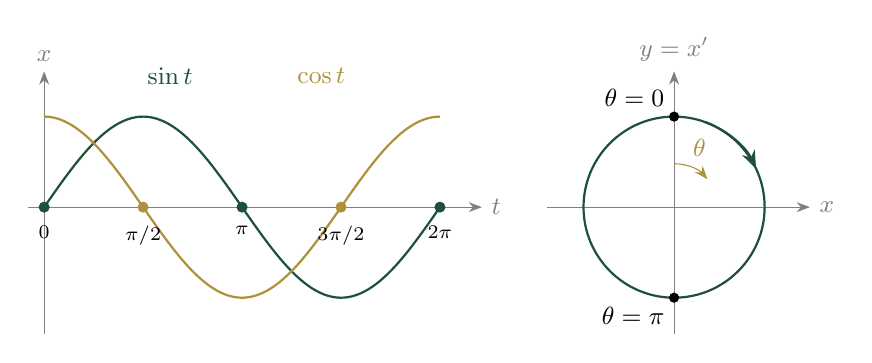
\begin{tikzpicture}[>=Stealth,font=\small]
\begin{scope}[x=.8cm,y=1.15cm]
 \draw[->,gray] (-.25,0)--(6.95,0) node[right]{$t$};
 \draw[->,gray] (0,-1.4)--(0,1.5) node[above]{$x$};
 \draw[GreenMain,thick,domain=0:6.2832,samples=100] plot (\x,{sin(\x r)});
 \draw[GoldMain,thick,domain=0:6.2832,samples=100] plot (\x,{cos(\x r)});
 \foreach \t/\lab in {0/0,1.5708/{\pi/2},3.1416/\pi,4.7124/{3\pi/2},6.2832/{2\pi}}{
  \draw (\t,.05)--(\t,-.05);\node[below,font=\scriptsize] at (\t,-.1){$\lab$};
 }
 \foreach \t in {0,3.1416,6.2832}{\fill[GreenMain] (\t,0) circle(2pt);}
 \foreach \t in {1.5708,4.7124}{\fill[GoldMain] (\t,0) circle(2pt);}
 \node[GreenMain] at (2,1.45){$\sin t$};\node[GoldMain] at (4.4,1.45){$\cos t$};
\end{scope}
\begin{scope}[shift={(8,0)},scale=1.15]
 \draw[->,gray] (-1.4,0)--(1.5,0) node[right]{$x$};
 \draw[->,gray] (0,-1.4)--(0,1.5) node[above]{$y=x'$};
 \draw[GreenMain,thick] (0,0) circle(1);
 \draw[GreenMain,->,thick] (70:1) arc[start angle=70,end angle=25,radius=1];
 \draw[GoldMain,->] (90:.48) arc[start angle=90,end angle=40,radius=.48];
 \node[GoldMain] at (.28,.65){$\theta$};
 \fill (0,1) circle(1.6pt) node[above left]{$\theta=0$};
 \fill (0,-1) circle(1.6pt) node[below left]{$\theta=\pi$};
\end{scope}
\end{tikzpicture}
\captionof{figure}{同一方程的独立解零点交错；右图中每经过一个零点，相位穿过一个 $k\pi$。}
\label{fig:ode-tikz-sturm-separation}
\end{minipage}
\end{center}

\section{比较定理与零点间距}
\begin{theorem}[Sturm 比较]
设 $Q,q$ 连续，$Q\geq q$。若 $x$ 解 $x''+qx=0$ 并以 $a<b$ 为相邻零点，
则每个非零解 $z$（$z''+Qz=0$）在 $[a,b]$ 至少有一个零点。
若 $Q>q$ 在 $[a,b]$ 上处处成立，则零点可取在 $(a,b)$。
\end{theorem}
\begin{proof}
将第一解的相位取为 $\alpha(a)=0,\alpha(b)=\pi$。
若第二解在某端点为零，闭区间版本已经成立。
否则改变其符号并选相位分支，使 $0<\beta(a)<\pi$。
设 $f_q(t,s)=\cos^2s+q(t)\sin^2s$，则
$\alpha'=f_q(t,\alpha),\beta'=f_Q(t,\beta)$。

令 $w=\beta-\alpha$，把差分精确写成
\[
 \begin{aligned}
 w'&=c(t)w+d(t),\\
 d(t)&=(Q(t)-q(t))\sin^2\alpha(t)\geq0,
\end{aligned}
\]
其中
\[
 c(t)=\displaystyle\int_0^1\partial_s f_Q(t,\alpha(t)+\tau w(t))\,d\tau
\]
为连续函数。常数变易给出
\[
 w(t)=e^{\int_a^tc}\left[w(a)+\int_a^te^{-\int_a^sc}d(s)\,ds\right].
\]
当 $w(a)>0$，方括号严格为正，因此 $\beta(b)>\pi$。
又 $\beta(a)<\pi$，故在开区间内取到 $\pi$，得到零点。
这证明了第二个解在两端均不为零时的结论，结合端点为零的情形，即得闭区间上的结论。

现在假设 $Q>q$。若第二解在左端点为零，取 $\beta(a)=0$，则 $w(a)=0$。
$\alpha$ 在 $a$ 后立即进入 $(0,\pi)$，因此 $d$ 在一个右邻域严格为正；
上式于是给出 $w(t)>0$ 对所有 $t>a$ 成立，特别是 $\beta(b)>\pi$。
所以除了左端零点以外，内部还有一次经过 $\pi$。
如果第二解仅在右端点为零，可从 $b$ 反向时间重复这一论证，
或把 $t$ 换成 $a+b-t$ 后应用左端情形，同样得到内部零点。
因此严格比较时零点可取在开区间。
\end{proof}
\begin{corollary}
若 $q\geq\omega^2>0$，则 $I$ 内相邻零点距离不超过 $\pi/\omega$；
当 $I$ 包含一条右半轴时，非零解还有任意大的零点。
若 $q\leq\Omega^2$，$\Omega>0$，则相邻零点距离不小于 $\pi/\Omega$。
若 $q\leq0$，每个非零解至多有一个零点。
\end{corollary}
\begin{proof}
常系数比较方程的零点间距分别是 $\pi/\omega$ 和 $\pi/\Omega$。
若存在超过相应界限的无零点区间，可在其内部放入比较解的两个相邻零点，
与比较定理矛盾。当 $I$ 包含右半轴时，把比较区间移到任意远处，
也得第一种情形的无限多个零点。
最后，若 $x$ 在 $a<b$ 为零，乘方程以 $x$ 并积分得
\[
 \int_a^b(x')^2\,\dd t=\int_a^bq(t)x(t)^2\,\dd t\leq0.
\]
所以 $x'=0$，由端点值知 $x=0$，与非零解矛盾。
\end{proof}
一般方程 $x''+p(t)x'+q(t)x=0$ 在 $p\in C^1$ 时，令
\[
 x=e^{-\frac12\displaystyle\int p}u,
\]
得到
$u''+(q-p'/2-p^2/4)u=0$。乘子从不为零，因此保持零点。

\section{Sturm--Liouville 问题}
\begin{definition}
给定连续实函数 $q$ 和 $l>0$，寻找
\[
 x''+(q(t)+\lambda)x=0,\qquad x(0)=x(l)=0
\]
的非零解，称为这里的 Sturm--Liouville 两点边值问题。
这样的 $\lambda$ 称特征值，相应非零解称特征函数。
\end{definition}
\begin{theorem}
特征值可以严格递增地排列为 $\lambda_1<\lambda_2<\cdots\to\infty$，
每个特征空间一维。第 $k$ 个特征函数在 $(0,l)$ 恰有 $k-1$ 个零点。
若 $m\leq q\leq M$，则
\[
 (k\pi/l)^2-M\leq\lambda_k\leq(k\pi/l)^2-m,
 \qquad \lambda_k/k^2\to(\pi/l)^2.
\]
\end{theorem}
\begin{proof}
\textbf{第一步：把边值问题化为一个相位方程。}
令 $x(t,\lambda)$ 解初值问题
\[
 x(0,\lambda)=0,\qquad x'(0,\lambda)=1.
\]
任何非零解若在左端为零，其左端导数必不为零，
除以该导数后便与 $x(t,\lambda)$ 具有相同初值，因此由唯一性重合。
所以每个特征空间一维，特征值条件正是 $x(l,\lambda)=0$。
取 $\theta(0,\lambda)=0$，这个条件等价于 $\theta(l,\lambda)=k\pi$，$k\geq1$。

\textbf{第二步：证明末端相位对参数严格增加。}
参数可微依赖定理给出 $w=\partial_\lambda x$，并由对方程求导得到
$w''+(q+\lambda)w=-x$、$w(0)=w'(0)=0$。
逐项计算为
\[
 (x'w-xw')'=x''w-xw''=x^2.
\]
零初值使 
\[
 x'w-xw'=\displaystyle\int_0^t x(s,\lambda)^2ds.
\]
又由相位角的微分公式，
\[
 \partial_\lambda\theta(l,\lambda)
 =\frac{x'(l,\lambda)w(l,\lambda)-x(l,\lambda)w'(l,\lambda)}
 {x(l,\lambda)^2+x'(l,\lambda)^2}>0.
\]
分母不为零，分子积分严格为正，因为 $x'(0,\lambda)=1$。

\textbf{第三步：确定相位的取值范围并编号。}
当 $\lambda\leq-\max q$ 时，$q+\lambda\leq0$。
解从零以正速度出发；在保持正值的阶段有 $x''=-(q+\lambda)x\geq0$，
所以导数不能降到零，解不可能再次为零。
因此末端相位位于 $(0,\pi)$。
另一方面，给定任意正整数 $N$，可取 $\lambda$ 足够大，使
$q+\lambda\geq\omega^2$ 且 $N\pi/\omega<l$。
比较定理使 $x$ 在 $[0,l]$ 有至少 $N$ 次零点穿越，故末端相位趋于无穷。
连续性与严格单调性说明每个水平 $k\pi$ 恰穿过一次，给出严格递增的 $\lambda_k$。
相邻零点角增为 $\pi$，故第 $k$ 个特征函数恰有 $k-1$ 个内部零点。
若 $\lambda_k$ 有有限聚点，末端相位在该紧参数区间有界，
但其值 $k\pi$ 无界，矛盾，所以 $\lambda_k\to\infty$。

\textbf{第四步：比较常系数方程以估计特征值。}
记 $\mu_k=(k\pi/l)^2$。
在 $\lambda=\mu_k-M$ 时有 $q+\lambda\leq\mu_k$，
由同初始角的标量比较，末端相位不超过常系数方程的 $k\pi$。
在 $\lambda=\mu_k-m$ 时有反向不等式，末端相位不小于 $k\pi$。
由末端相位严格随 $\lambda$ 增加，得到
$\mu_k-M\leq\lambda_k\leq\mu_k-m$。
两边除以 $k^2$ 后，常数误差趋于零，夹逼得到所述渐近式。
\end{proof}

\begin{definition}[平方平均空间与完全性]\label{def:l2-completion}
先在闭区间上的连续实函数空间 $C([0,l])$ 上定义
\[
 \langle f,g\rangle=\int_0^l f(t)g(t)\,dt,
 \qquad\|f\|_2=\langle f,f\rangle^{1/2}.
\]
将这个内积空间按 $\|\cdot\|_2$ 完备化，得到 $L^2(0,l)$。
具体地，它的元素可由连续函数的 Cauchy 列表示；两列等价，是指它们之差的 $2$ 范数趋于零。
内积定义为代表列内积的极限，Cauchy--Schwarz 不等式保证该极限存在且与代表列无关。
一个正交系的有限线性组合在 $2$ 范数下稠密时，称该正交系完全。
本节出现的特征函数都是经典光滑函数，因此其内积直接用上面的通常积分计算。
\end{definition}

\begin{proposition}
不同特征值的实特征函数在 $L^2(0,l)$ 中正交。
\end{proposition}
\begin{proof}
分别把两方程乘以另一个解后相减积分，得到
\[
 (\lambda_i-\lambda_j)\int_0^lx_i x_j\,\dd t
 =[x_i x_j'-x_i'x_j]_0^l=0.
\]
端点条件使边界项消失，而特征值不同，所以积分为零。
\end{proof}
\begin{definition}[权内积与形式自伴]
对连续正权 $w$，权内积为 $\langle f,g\rangle_w=\displaystyle\int_0^l wf g\,dt$。
表达式 $Ly=-w^{-1}[(py')'+qy]$ 配上零端点条件时，
两次分部积分给出 $\langle Lf,g\rangle_w=\langle f,Lg\rangle_w$；这称其在该边界条件下形式自伴。
这里“形式”指对光滑零端点函数的积分恒等式，不省略无穷维算子定义域的问题。
\end{definition}
方程 $(p x')'+(q+\lambda w)x=0$（$p\in C^1$，$q,w$ 连续且 $p,w>0$）
宜取相平面坐标 $(x,px')$；同样的 Wronskian 与相位比较可以使用，正交性采用上述权内积。

\setchapterimage{figure/Chapter9封面图.jpg}
\setchapterintro{本章讨论周期系数微分方程。先利用单周期映射判断周期解的存在性与稳定性，再研究参数共振、倒立摆的振动稳定以及受迫振动。}
\chapter{周期系统、单周期映射与振动}\label{chap:periodic}

第六章的 Poincar\'e 映射由解与横截面的相邻两次交点确定。对于周期系数方程，可以考察解经过一个周期后的值，由此定义单周期映射，再利用第三章的标准解矩阵及第六章的稳定性判据研究它的迭代。

\section{单周期映射}
设 $f(t+T,x)=f(t,x)$，$T>0$，并假定下文所用的解全局存在。
记从时刻 $s$ 的初值确定时刻 $t$ 的解值的映射为 $P_{t,s}$。
\begin{definition}
映射 $M=P_{T,0}$ 称为单周期映射。线性系统 $x'=A(t)x$ 时，
若 $X(0)=I$，则 $M=X(T)$ 是单周期矩阵，其特征值称为乘子。
\end{definition}
\begin{theorem}
\[
 \begin{aligned}
 P_{t+T,s+T}&=P_{t,s},\\
 P_{nT,0}&=M^n,\\
 P_{nT+s,0}&=P_{s,0}M^n\qquad(0\leq s\leq T).
\end{aligned}
\]
$T$ 周期解与 $M$ 的不动点一一对应；解的 Lyapunov 稳定性及渐近稳定性，
分别等价于该不动点对迭代 $M^n$ 的相同性质。
\end{theorem}
\begin{proof}
若 $x(t)=P_{t,s}\xi$，则 $z(t)=x(t+T)$ 满足
$z'=f(t+T,z)=f(t,z)$，且 $z(s)=x(s+T)$。
对在 $s+T$ 取初值 $\xi$ 的解作这一平移，由唯一性得到
$P_{t+T,s+T}\xi=P_{t,s}\xi$。再由解映射的复合关系，
\[
 P_{(n+1)T,0}=P_{(n+1)T,nT}P_{nT,0}=MP_{nT,0}.
\]
从 $P_{0,0}=I$ 归纳得 $P_{nT,0}=M^n$，继而
\[
 P_{nT+s,0}=P_{nT+s,nT}M^n=P_{s,0}M^n.
\]
若 $M\xi=\xi$，解 $x(t+T)$ 与 $x(t)$ 在 $t=0$ 取同一初值，
唯一性使它们相同；反之，对周期解取 $t=0,T$ 即得不动点条件。

记不动点为 $\xi_*$，对应周期解 $x_*(s)=P_{s,0}\xi_*$。
周期解稳定时，在时刻 $t=nT$ 取解值，即得相应不动点对迭代的稳定性。
反向证明中，固定 $\epsilon>0$。映射 $(s,\xi)\mapsto P_{s,0}\xi$
在紧集 $[0,T]\times\{\xi_*\}$ 附近连续。用有限覆盖，存在 $\eta>0$，使
\[
 |\xi-\xi_*|<\eta\ \Longrightarrow\
 \sup_{0\leq s\leq T}|P_{s,0}\xi-P_{s,0}\xi_*|<\epsilon.
\]
迭代不动点的稳定性给出 $\delta>0$，使 $|\xi-\xi_*|<\delta$ 时，对一切 $n\geq0$
均有 $|M^n\xi-\xi_*|<\eta$。将 $M^n\xi$ 代入上式，结合周期分解，
便得到每个时刻 $t=nT+s$ 的解的估计，从而证明周期解稳定。

若该不动点还吸引附近的迭代序列，则 $M^n\xi\to\xi_*$。
对任意 $\epsilon>0$，充分大的所有 $n$ 均满足上述 $\eta$ 条件，
故整段 $[nT,(n+1)T]$ 上的解差均小于 $\epsilon$。
这证明周期解还具有吸引性。反过来，只需考察整数倍周期时刻的解值，即得迭代不动点的吸引性，因此两种渐近稳定性等价。
\end{proof}
线性性由解的叠加得到。Liouville 公式还给出
\[
 \det M=\exp\int_0^T\operatorname{tr}A(t)\,\dd t.
\]
\begin{proposition}[一维乘子]
对 $y'=a(t)y$，$a(t+T)=a(t)$，乘子为
\[
 \mu=\exp\displaystyle\int_0^Ta(t)\,\dd t>0.
\]
$\mu<1$ 时所有解趋于零，$\mu>1$ 时每个非零解的绝对值趋于无穷，
$\mu=1$ 时所有解均为 $T$ 周期。
\end{proposition}
\begin{proof}
显式解给出 $y(t+T)=\mu y(t)$。
在 $[0,T]$ 上，连续正函数 $\exp\displaystyle\int_0^sa$ 有正的上下界，
所以整个正半轴的行为由 $\mu^n$ 决定，而不只是整数周期时刻的行为。
\end{proof}
\begin{theorem}[周期非齐次方程]
对 $y'=a(t)y+b(t)$，若 $a,b$ 均 $T$ 周期且 $\displaystyle\int_0^Ta\ne0$，
则存在唯一 $T$ 周期解；它在 $\mu<1$ 时渐近稳定，$\mu>1$ 时不稳定。
\end{theorem}
\begin{proof}
由常数变易，$M(y)=\mu y+c$，其中 $c$ 是零初值经过一周期的值。
$\mu\ne1$ 时唯一不动点为 $y_*=c/(1-\mu)$，故对应唯一周期解。
任意解与该周期解之差满足齐次方程，稳定性由前一命题得到。
$\mu=1$ 时可能无周期解，也可能所有解周期，取决于 $c$ 是否为零，故不能删掉假设。
\end{proof}

\paragraph{与极限环返回映射的结合。}
在自治闭轨附近取角向坐标 $s\bmod T$ 和横向坐标 $u$，方程可写
$du/ds=a(s,u)$，$a(s,0)=0$。
其横向线性化为 $v'=a_u(s,0)v$。
由前文初值导数的变分方程，返回映射的导数就是其乘子
$\exp\displaystyle\int_0^Ta_u(s,0)\,\dd s$。
这把已有 Poincaré 导数判据与本章的周期线性方程联系起来。
若该乘子不同于 1，小扰动后的返回方程 $P_\varepsilon(u)-u=0$ 可由隐函数定理解出，
所以闭轨继续存在；乘子等于 1 时这种推断不再有效。

\section{二维保面积系统与强稳定}
\begin{definition}
线性周期系统 $x'=A(t)x$ 在二维且 $\operatorname{tr}A(t)=0$ 时，
本章称为线性 Hamilton 系统。其单周期矩阵保持面积。
若零解稳定，且每个充分接近的同周期线性 Hamilton 系统的零解仍稳定，称为强稳定。
接近性采用系数矩阵在 $[0,T]$ 上的一致范数。
\end{definition}
\begin{theorem}[迹判据]
设实 $2\times2$ 矩阵 $M$ 满足 $\det M=1$。
当 $|\operatorname{tr}M|<2$ 时迭代稳定；当 $|\operatorname{tr}M|>2$ 时不稳定。
在等号情形，稳定当且仅当 $M=I$ 或 $M=-I$。
\end{theorem}
\begin{proof}
二维矩阵的特征多项式为
\[
 p(\lambda)=\lambda^2-(\operatorname{tr}M)\lambda+1.
\]
先说明迭代稳定等价于 $\sup_{n\geq0}\|M^n\|<\infty$。
若该上界为 $C$，取 $|x_0|<\epsilon/(C+1)$ 即得稳定性。
反之，若零点稳定，对 $\epsilon=1$ 取稳定半径 $\delta$，
将任意单位向量乘以 $\delta/2$，便得 $\|M^n\|\leq2/\delta$。

当 $|\operatorname{tr}M|<2$，判别式为负，两根共轭，乘积为 1，故都在单位圆上。
写一根为 $e^{i\theta}$，$\sin\theta\ne0$。取复特征向量的实部与虚部为实基，
$M$ 的实矩阵为一个旋转矩阵，因而在此基下所有幂的范数均为 1。
换回原基仅引入固定常数，故稳定。

当 $|\operatorname{tr}M|>2$，两根实且互为倒数，并且至少一根 $\lambda$ 满足
$|\lambda|>1$。沿对应的实特征向量 $v$，有 $M^nv=\lambda^nv$，故不稳定。

最后设 $\operatorname{tr}M=2s$，其中 $s=1$ 或 $-1$。Hamilton--Cayley 公式给出
$(M-sI)^2=0$。若 $M=sI$，幂显然有界。否则写 $M=sI+N$，
$N\ne0,N^2=0$，则
\[
 M^n=s^nI+ns^{n-1}N.
\]
选 $v$ 使 $Nv\ne0$，反三角不等式给出
\[
 |M^nv|\geq n|Nv|-|v|\to\infty,
\]
故不稳定。这穷尽全部情形。
\end{proof}
\begin{corollary}
若单周期矩阵满足 $|\operatorname{tr}M|<2$，则零解强稳定。
\end{corollary}
\begin{proof}
设 $A,\widetilde A$ 为两个同周期系数矩阵，$X(0)=\widetilde X(0)=I$。
固定 $B>\sup_{[0,T]}\|A(t)\|$，并限制扰动，使 $\|\widetilde A(t)\|\leq B$。
由积分方程和 Gronwall 不等式，$\|X(t)\|,\|\widetilde X(t)\|\leq e^{Bt}$。
设 $\eta=\sup_{[0,T]}\|A-\widetilde A\|$，作差得
\[
 \|X(t)-\widetilde X(t)\|
 \leq B\int_0^t\|X(s)-\widetilde X(s)\|\,ds
       +\eta\int_0^te^{Bs}\,ds.
\]
再次使用 Gronwall，或逐次代入积分不等式，得到
\[
 \|X(t)-\widetilde X(t)\|\leq\eta t e^{Bt}.
\]
特别地，
\[
 \|M-\widetilde M\|\leq\eta T e^{BT},
\]
故单周期矩阵连续依赖系数。

令 $\gamma=2-|\operatorname{tr}M|>0$。迹是矩阵元的连续函数，
所以 $\eta$ 足够小时有
\[
 |\operatorname{tr}\widetilde M-\operatorname{tr}M|<\gamma/2,
\]
从而
$|\operatorname{tr}\widetilde M|<2$。
扰动仍在迹零的 Hamilton 系统类内，Liouville 公式保证
$\det\widetilde M=1$。迹判据说明每个这种邻近系统的离散迭代稳定，
再由前面证明的周期解与迭代不动点的稳定性等价关系，得到零解稳定，故原零解强稳定。
\end{proof}
注意 $x''+a(t)x=0$ 的状态矩阵始终迹为零，所以其零解对任何 $a$ 均不可能渐近稳定。
否则两个独立初值的像都趋于零，所张成平行四边形的面积也趋于零，
与恒等于 1 的 Wronskian 矛盾。


图~\ref{fig:ode-tikz-monodromy-trace} 展示乘子随迹所处区间的三种位置；边界 $\pm2$ 仍须检查 Jordan 块。
\begin{center}
\begin{minipage}{0.96\linewidth}
\centering
% TikZ mathematical illustration; compiled with the main document.
\begin{tikzpicture}[>=Stealth,font=\small]
 \draw[->,gray] (-5,0)--(5.2,0) node[right]{$\operatorname{tr}M$};
 \draw[GreenMain,line width=2pt] (-1.8,0)--(1.8,0);
 \foreach \x/\lab in {-1.8/-2,1.8/2}{\draw (\x,.1)--(\x,-.1);\node[below]at(\x,-.1){$\lab$};}
 \node[GreenMain] at (0,.45){稳定};
 \node[GoldMain] at (-3.5,.45){不稳定};\node[GoldMain] at (3.5,.45){不稳定};
 \foreach \shift in {-3.5,0,3.5}{
  \begin{scope}[shift={(\shift,2)}]
   \draw[gray,dashed] (0,0) circle(.75);\draw[gray] (-1.35,0)--(1.35,0);
  \end{scope}
 }
 \fill[GoldMain] (-4.7,2) circle(2pt);\fill[GoldMain] (-3.96875,2) circle(2pt);
 \fill[GreenMain] ({.75*cos(55)},{2+.75*sin(55)}) circle(2pt);
 \fill[GreenMain] ({.75*cos(55)},{2-.75*sin(55)}) circle(2pt);
 \fill[GoldMain] (4.7,2) circle(2pt);\fill[GoldMain] (3.96875,2) circle(2pt);
 \node at (-3.5,3.1){负实互逆乘子};\node at (0,3.1){共轭单位乘子};\node at (3.5,3.1){正实互逆乘子};
\end{tikzpicture}
\captionof{figure}{二维保面积单周期矩阵的迹判据：稳定区间为 $|\operatorname{tr}M|<2$。}
\label{fig:ode-tikz-monodromy-trace}
\end{minipage}
\end{center}

\section{参数共振与振动稳定}
考虑
\[
 x''+\omega^2(1+\varepsilon a(t))x=0,
 \qquad a(t+2\pi)=a(t).
\]
\begin{definition}
因系数的周期改变使原来稳定的振动变为不稳定，称为参数共振。
这与在方程右端施加外部周期力的受迫共振不同。
$a(t)=\cos t$ 的方程称 Mathieu 型方程。
\end{definition}
\begin{theorem}
当 $\varepsilon=0$ 且 $\omega>0$ 不为整数或半整数时，系统强稳定。
所以不稳定区域趋近 $\varepsilon=0$ 轴时，只能在 $\omega=k/2$ 处接触该轴。
\end{theorem}
\begin{proof}
未扰动单周期矩阵为
\[
 R_\omega(2\pi)=
 \begin{pmatrix}
 \cos2\pi\omega&\sin2\pi\omega/\omega\\
 -\omega\sin2\pi\omega&\cos2\pi\omega
 \end{pmatrix}.
\]
其迹为 $2\cos2\pi\omega$，在所述点严格位于 $(-2,2)$。
强稳定性保证这些点都有不含不稳定系统的邻域。
上述结论只确定不稳定区域与参数轴相交的可能位置；各处是否存在不稳定区域，还须进一步计算。
\end{proof}

\begin{proposition}[分段常系数计算]
若一个周期的前后两段分别满足 $x''+\omega_1^2x=0$、$x''+\omega_2^2x=0$，
各段时间为 $\tau_1,\tau_2$，则
\[
 M=R_{\omega_2}(\tau_2)R_{\omega_1}(\tau_1),
\]
且
\[
 \operatorname{tr}M=2\cos(\omega_1\tau_1)\cos(\omega_2\tau_2)
 -\left(\frac{\omega_1}{\omega_2}+\frac{\omega_2}{\omega_1}\right)
 \sin(\omega_1\tau_1)\sin(\omega_2\tau_2).
\]
\end{proposition}
\begin{proof}
每段由已证常系数矩阵指数公式给出 $R_{\omega_i}$，先作用第一段再作用第二段，
故乘积次序如上。计算乘积的两个对角元并相加得到迹。
因此稳定边界可直接由该迹等于 $\pm2$ 求出。
\end{proof}
例如取 $\tau_1=\tau_2=\pi$、$\omega_{1,2}=\omega\pm\varepsilon$，展开正弦余弦即可
观察到半整数附近比整数附近更宽的不稳定区。
具体地，当 $\omega=k+1/2+\eta$，$k\geq0$，展开到二次阶有
\[
 \operatorname{tr}M=-2+4\pi^2\eta^2-
 \frac{4\varepsilon^2}{(k+1/2)^2}+o(\eta^2+\varepsilon^2).
\]
因此边界一阶为
\[
 \eta=\pm\varepsilon/[\pi(k+1/2)]+o(\varepsilon).
\]
该式来自 
\[
 \omega_1/\omega_2+\omega_2/\omega_1
=2+4\varepsilon^2/\omega^2+O(\varepsilon^4),
\]
以及
\[
 2\cos a\cos b-2\sin a\sin b=2\cos(a+b).
\]

\begin{example}[倒立摆的快速悬点振动]
考虑分段恒加速度的悬点振动模型。摆长 $l$，悬点位移振幅 $a$，
每半周期 $\tau$ 内加速度为 $\pm c$，其中 $c=8a/\tau^2$。
倒立位置的线性化为 $x''=(\omega^2\pm\alpha^2)x$，
$\omega^2=g/l,\alpha^2=c/l$。当 $\alpha>\omega$，令
$k=\sqrt{\alpha^2+\omega^2}$、$\Omega=\sqrt{\alpha^2-\omega^2}$。
\end{example}
\begin{proposition}
此线性周期系统的单周期迹为
\[
 2\cosh(k\tau)\cos(\Omega\tau)
 +\left(\frac{k}{\Omega}-\frac{\Omega}{k}\right)
 \sinh(k\tau)\sin(\Omega\tau).
\]
当 $a/l$ 为充分小的固定正数、$\tau$ 再充分小时，该迹严格位于 $(-2,2)$，故线性零解稳定。
\end{proposition}
\begin{proof}
第一段的双曲矩阵为
\[
 \begin{pmatrix}
  \cosh(k\tau)&\sinh(k\tau)/k\\
  k\sinh(k\tau)&\cosh(k\tau)
 \end{pmatrix},
\]
第二段为 $R_\Omega(\tau)$。相乘取迹即得公式。
记 $s=\alpha^2\tau^2=8a/l$、$d=\omega^2\tau^2$。
在 $\tau\to0$ 即 $d\to0$ 时，迹趋于
\[
 2\cosh\sqrt s\cos\sqrt s=2-s^2/3+O(s^4).
\]
对充分小固定 $s>0$，此极限小于 2 且大于 $-2$。
连续性使足够小的 $d$ 保持该严格不等式。
这里证明了快速悬点振动可以稳定倒立位置的线性化；非线性情形不能只用纯虚谱就判稳定。
\end{proof}

\section{复振幅、共振与拍}
对实常系数算子 $P(D)$，若 $P(D)z=F$，则
$P(D)\operatorname{Re}z=\operatorname{Re}F$，由实系数线性性直接成立。
\begin{definition}
表示 $\operatorname{Re}(Ce^{i\nu t})$ 的复数 $C=re^{i\theta}$ 称复振幅；
$r$ 是振幅，$\theta$ 是相位。
\end{definition}
\begin{proposition}
对 $x''+kx'+\omega^2x=\cos\nu t$，$k>0,\omega>0$，稳态复振幅为
\[
 \begin{aligned}
 C(\nu)&=\frac1{\omega^2-\nu^2+ik\nu},\\
 r(\nu)&=\frac1{\sqrt{(\omega^2-\nu^2)^2+k^2\nu^2}}.
\end{aligned}
\]
任意解与该稳态振动之差趋于零。
\end{proposition}
\begin{proof}
把特解 $Ce^{i\nu t}$ 代入复方程，其左边为
$(\omega^2-\nu^2+ik\nu)Ce^{i\nu t}$，故得到 $C$。
取模即得振幅。齐次特征根实部均负，因此由前文常系数稳定判据，
任意齐次解衰减到零。
\end{proof}
曲线 $\nu\mapsto P(i\nu)$ 称此处的 Mikhailov 曲线；
$\nu\mapsto1/P(i\nu)$ 称幅相特性。倒数变换同时给出振幅和相位。
当 $k$ 很小，$r$ 的峰值位于接近 $\omega$ 处，量级为 $1/(k\omega)$。
事实上对分母平方求导，其非零驻点满足 $\nu^2=\omega^2-k^2/2$，
代回可得峰值 $[k\sqrt{\omega^2-k^2/4}]^{-1}$（此式要求 $k^2<2\omega^2$）。

\begin{proposition}[无阻尼极限]
对 $x''+\omega^2x=\cos\nu t$，$\nu\ne\omega$ 时零初值解为
\[
 x(t)=\frac{\cos\nu t-\cos\omega t}{\omega^2-\nu^2}.
\]
两频率接近时出现拍；当 $\nu\to\omega$ 时该解趋于
$t\sin\omega t/(2\omega)$，振幅线性增长。
\end{proposition}
\begin{proof}
代入并检查 $x(0)=x'(0)=0$ 即得前式。
用余弦差公式，分子等于
$-2\sin((\nu+\omega)t/2)\sin((\nu-\omega)t/2)$，
其中第二因子缓慢变化，这就是拍的振幅包络。
对参数取极限或用一阶 Taylor 公式得共振解，亦可直接代入验证。
\end{proof}

\section{弱非线性周期的参数展开}
前文的 $C^r$ 依赖定理允许在有界时间段内按初振幅展开解，
但不自动允许把有界时间近似延伸到任意长时间。
对摆初值 $x(0)=A,x'(0)=0$，写
\[
 x(t,A)=A x_1(t)+A^3x_3(t)+O(A^5).
\]
由方程在 $x\mapsto-x$ 下的对称性，偶次项为零。
比较 $A$ 的系数得 $x_1=\cos t$；比较三次项得
\[
 x_3''+x_3=\frac16\cos^3t
 =\frac18\cos t+\frac1{24}\cos3t,
 \qquad x_3(0)=x_3'(0)=0.
\]
直接求解并代回检查可得
\[
 x_3(t)=\frac{\cos t-\cos3t}{192}+\frac{t\sin t}{16}.
\]
一阶谐波的时间增长项与
\[
 \cos((1-A^2/16)t)=\cos t+(A^2/16)t\sin t+O(A^4)
\]
 相符，
说明频率下降。为了严密提取周期，可考察 $x'$ 在接近 $2\pi$ 的零点：
将 $x'/A$ 光滑延拓到 $A=0$，其在 $(t,A)=(2\pi,0)$ 对 $t$ 的导数为 $-1$。
隐函数定理给出回到右转向点的时间 $T(A)$。
将 $T=2\pi+cA^2+O(A^4)$ 代入 $x'/A=0$，得到
$-c+2\pi/16=0$。所以
\[
 T(A)=2\pi(1+A^2/16+O(A^4)),
\]
与上一章直接由周期积分得到的结论一致。

\setchapterimage{figure/Chapter10封面图.jpg}
\setchapterintro{相图分类必须先说明允许怎样改变坐标。本章区分线性、可微与拓扑共轭，构造用于判定稳定性的 Lyapunov 二次型，再研究纯虚谱带来的环面运动。}
\chapter{线性系统的共轭分类与环面运动}\label{chap:linear-conjugacy}

第四章和第六章已经按 Jordan 结构计算并分类线性解，第~\ref{chap:arnold-geometry}~章又说明坐标变换如何改变向量场。本章分别讨论线性变换、微分同胚和同胚下的等价关系，并给出相应的分类条件。

\section{三种等价关系}
\begin{definition}
流 $\varphi^t,\psi^t$ 若满足
$h\varphi^t=\psi^th$，称被 $h$ 共轭。
当 $h$ 分别为线性同构、$C^1$ 微分同胚、同胚时，称线性等价、可微等价、拓扑等价。
同胚是自身和逆均连续的双射。这里始终保留同一个时间 $t$，
区别于只把定向轨道映成定向轨道的轨道等价。
\end{definition}
\begin{theorem}
实线性系统 $x'=Ax,y'=By$ 线性等价当且仅当 $A,B$ 相似。
它们可微等价当且仅当线性等价。
\end{theorem}
\begin{proof}
线性换元 $y=Hx$ 给出 
\[
 B=HAH^{-1},
\]
充分性也由同式直接验证。
若 $h$ 为可微共轭，令 $c=h(0)$。由 $Be^{tB}c=Bc=0$ 或直接固定点性质知 $Bc=0$。
平移 $h$ 为 $h_1(x)=h(x)-c$，则它仍共轭并固定零点。
对 $h_1e^{tA}=e^{tB}h_1$ 在 $x=0$ 求导，得
\[
 He^{tA}=e^{tB}H,
\]
其中 $H=Dh_1(0)$ 可逆。
再对 $t=0$ 求导，得到 $HA=BH$，即相似。
\end{proof}
简单谱时相似类由相同的特征值决定；重根时还要比较 Jordan 块。
例如 $I$ 与 $\left(\begin{smallmatrix}1&1\\0&1\end{smallmatrix}\right)$ 特征值相同却不相似。

\section{Lyapunov 二次型与拓扑分类}
\begin{definition}
矩阵无实部为零的特征值时称为双曲。
所有负实部广义特征空间的实直和称为稳定子空间 $E^s$，正实部对应者称为不稳定子空间 $E^u$。
记其维数为 $m_-,m_+$。
\end{definition}
由前文的广义特征空间分解，$\R^n=E^s\oplus E^u$，且这两个子空间均不变。
在 $E^s$ 上 $e^{tA}x\to0$（$t\to+\infty$），在 $E^u$ 上反向时间趋于零。

\begin{lemma}[几乎特征基]
复矩阵 $A$ 对任意 $\varepsilon>0$ 都存在一组基，使矩阵上三角且每个严格上三角元的绝对值小于 $\varepsilon$。
\end{lemma}
\begin{proof}
先由 Jordan 形取上三角基 $e_1,\ldots,e_n$，再令 $e_j'=\delta^je_j$。
新矩阵元为 $a'_{ij}=a_{ij}\delta^{j-i}$。
当 $j>i$，选足够小 $\delta>0$ 使所有这些有限个元同时小于 $\varepsilon$。
对角元保持为特征值，下三角仍为零。
\end{proof}
\begin{lemma}[正定二次型的开性]
若 $Q$ 为正定二次型，则存在 $c,C>0$，使
$c|x|^2\leq Q(x)\leq C|x|^2$；系数足够小的二次型扰动仍正定。
\end{lemma}
\begin{proof}
在单位球面上 $Q$ 连续且严格为正，由紧性取到正的最小值和有限最大值。
齐次性给出上下界。
若扰动各系数绝对值不超过 $\eta$，单位球面上的扰动绝对值不超过 $n^2\eta$，
取其小于 $c$ 即可。
\end{proof}
\begin{theorem}[Lyapunov 椭球]
若 $A$ 的全部特征值实部为正，则存在正定实二次型 $Q$，使
$L_{Ax}Q$ 正定。因此存在 $0<c<C$，满足
\[
 cQ(x)\leq L_{Ax}Q(x)\leq CQ(x).
\]
负实部情形，对 $-A$ 应用同一结论即可。
\end{theorem}
\begin{proof}
令 $\gamma=\min_j\operatorname{Re}\lambda_j>0$。
在几乎特征基中，严格上三角元都可取为绝对值不超过 $\eta$。
设 $Q(z)=\sum_j|z_j|^2$，沿 $z'=Az$ 有
\[
 \dot Q=2\sum_j\operatorname{Re}\lambda_j|z_j|^2
 +2\operatorname{Re}\sum_{i<j}a_{ij}z_j\overline z_i.
\]
利用 $2|z_i||z_j|\leq|z_i|^2+|z_j|^2$，交叉项绝对值满足
\[
 \left|2\operatorname{Re}\sum_{i<j}a_{ij}z_j\overline z_i\right|
 \leq\eta\sum_{i<j}(|z_i|^2+|z_j|^2)
 =\eta(n-1)Q(z).
\]
故取 $\eta(n-1)<\gamma$ 即有 $\dot Q\geq\gamma Q$（$n=1$ 时无交叉项）。
上界同理由有限个矩阵元得到，例如
$\dot Q\leq[2\max_j\operatorname{Re}\lambda_j+\eta(n-1)]Q$。

虽然构造使用了复基，原实空间在复化后仍是一个实线性子空间，且在实矩阵 $A$ 下不变。
将 $Q$ 限制在该子空间，再用原来的实坐标表示，就得到实正定二次型。
上述沿流导数不等式在限制后仍成立。
若上界常数与下界相同，可将下界减半、上界增大，取得所需 $0<c<C$。
\end{proof}
\begin{theorem}[双曲线性系统的拓扑分类]\label{thm:arnold-linear-topology}
两个同维双曲实线性系统拓扑共轭，当且仅当 $m_-$ 相同。
\end{theorem}
\begin{proof}
先设全部特征值实部为正，取 Lyapunov 二次型 $Q$，令 $S=\{Q=1\}$。
对非零 $x$ 记 $q(t)=Q(e^{tA}x)>0$。导数估计给出
$c\leq (\log q)'\leq C$。因此对 $t\geq0$，
\[
 e^{ct}Q(x)\leq Q(e^{tA}x)\leq e^{Ct}Q(x),
\]
对 $t\leq0$ 则有 
\[
 e^{Ct}Q(x)\leq Q(e^{tA}x)\leq e^{ct}Q(x).
\]
所以 $q$ 严格递增，负向趋零、正向趋无穷。介值定理和严格单调性说明
每条非零轨道恰经过 $S$ 一次，且每个非零点唯一写成 $x=e^{tA}\xi$，$\xi\in S$。

以此表示定义 $h(e^{tA}\xi)=e^t\xi$，并置 $h(0)=0$。
因为每条从零点出发的射线也恰交 $S$ 一次，$e^t\xi$ 同样唯一表示任意非零点，
故 $h$ 是双射。确定时间的方程为 
\[
 Q(e^{-tA}x)=1,
\]
其对 $t$ 的导数
为 $-L_{Ax}Q(e^{-tA}x)<0$。隐函数定理保证 $t=t(x)$ 在非零点光滑，
$\xi=e^{-t(x)A}x$ 亦然；逆映射由射线坐标给出，也在非零点连续。

还须检查零点。若 $x=e^{tA}\xi\to0$，则 $Q(x)\to0$，最终 $t<0$。
上面的估计给出 $e^{Ct}\leq Q(x)$，故
\[
 t\leq C^{-1}\log Q(x)\to-\infty.
\]
椭球 $S$ 紧，因而 $h(x)=e^t\xi\to0$。
反之，若 $y=e^t\xi\to0$，$S$ 上的 Euclidean 长度有正常数下界，故 $t\to-\infty$；
再由 $Q(e^{tA}\xi)\leq e^{ct}$ 得 $h^{-1}(y)\to0$。
因此 $h$ 在全空间为同胚。最后直接计算
\[
 h(e^{sA}e^{tA}\xi)=e^{t+s}\xi=e^sh(e^{tA}\xi),
\]
故它将原系统共轭到 $y'=y$，且时间参数保持不变。

对负实部部分反向时间，得到与 $u'=-u$ 的共轭。
一般双曲系统分解为稳定与不稳定两个不变子空间，在各部分应用上述构造，
再取两个同胚的直积，得到标准系统 $u'=-u,v'=v$。
两个系统的稳定维数相同且总维数相同，便有同一个标准系统，充分性得证。

反过来，设存在共轭。双曲矩阵可逆，所以两系统的唯一平衡点均为零，共轭必固定零。
由连续性，$e^{tA}x\to0$ 蕴含 $e^{tB}h(x)\to0$；应用逆共轭得反向蕴含。
对于双曲线性系统，趋零点集恰为稳定子空间：不稳定分量只要非零，正向就不能趋零。
于是共轭将 $E_A^s$ 同胚到 $E_B^s$。由拓扑维数不变性
（Euclidean 空间 $\R^p,\R^q$ 同胚必有 $p=q$），两稳定维数相同。
\end{proof}
上述共轭通常不是可微的。比如一维 $x'=x$ 与 $y'=2y$ 可由
$y=\operatorname{sgn}(x)|x|^2$ 共轭，但逆在零点不可微。
平面稳定焦点与稳定结点也拓扑共轭，尽管不是线性共轭。

\begin{remark}[非线性情形的边界]
非线性双曲平衡点附近也存在保持时间的局部拓扑共轭。该结论称为 Hartman--Grobman 定理，其证明将在不变流形与进阶专题一章给出。
\end{remark}

\section{纯虚谱、不变环面与周期不变量}
\begin{proposition}
共轭保持每条非恒定周期解的最小正周期。
因此两个二维线性中心 $x''+\omega_i^2x=0$（$\omega_i>0$）
在保持时间参数不变的拓扑共轭下等价，当且仅当 $\omega_1=\omega_2$。
\end{proposition}
\begin{proof}
若 $\varphi^T(x)=x$，共轭给出 $\psi^T(hx)=hx$。
应用逆共轭，两个点的周期集合相同，最小正周期相同。
中心的所有非零轨道最小周期为 $2\pi/\omega_i$，故必要性成立；
频率相同时两个矩阵实相似，给出充分性。
\end{proof}
\begin{definition}
$m$ 维环面为 $\mathbb T^m=(\R/2\pi\Z)^m$。
环面上的线性流为 $\theta(t)=\theta_0+\omega t\pmod{2\pi}$。
频率 $\omega_1,\ldots,\omega_m$ 称为有理独立，若
$k\cdot\omega=0$、$k\in\Z^m$ 只能推出 $k=0$。
\end{definition}

\begin{definition}[半单特征值]
特征值称半单，是指它在复 Jordan 形中的所有对应块均为一阶；等价地，其特征子空间维数等于它在特征多项式中的重数。
所有特征值的集合称矩阵的谱，“纯虚谱”指所有特征值实部为零。
环面 $\mathbb T^m$ 取圆周的乘积拓扑，其函数可用每个角变量均为 $2\pi$ 周期的函数表示。
\end{definition}

实线性系统在纯虚特征值均半单时分成若干独立旋转平面。
固定各平面非零振幅得到不变环面；振幅为零的平面不贡献一个圆因子。
若重特征值不是半单的，解中可能出现 $t\sin\omega t$ 等项，此时解未必有界，因而不一定存在上述不变环面。

\begin{lemma}[无理旋转]
若 $\alpha/(2\pi)$ 无理，则序列 $\theta+n\alpha\pmod{2\pi}$（$n\geq0$）在圆上稠密。
\end{lemma}
\begin{proof}
先看整数 $n\in\Z$ 的全部轨道，其闭包为圆的闭子群的一个陪集。
把 $N+1$ 个点放入 $N$ 个等分弧，抽屉原理给出非零整数倍角度距零小于 $2\pi/N$。
无理性确保这个距离不为零；任意小步长的整数倍能逼近圆上任一点，
所以双向轨道稠密。
还须说明负次迭代也在正次轨道的闭包中。
紧性给出越来越大的正整数 $n_j$，使 $n_j\alpha\pmod{2\pi}\to0$；
若这样的回归整数有界，无理性将被违反。
对固定正整数 $r$，$(n_j-r)\alpha\to-r\alpha$，且最终 $n_j-r\geq0$。
所以负次点也在正次闭包中，正向稠密性成立。
\end{proof}
无理性在这里保证了小步长不为零；回归序列则把双向轨道的稠密性转为正向轨道的稠密性。

\begin{theorem}[二维环面]
若非零频率 $\omega_1,\omega_2$ 有理相关，则所有环面轨道闭合；
若有理独立，则每条轨道在整个二维环面稠密。
\end{theorem}
\begin{proof}
有理相关时存在 $T>0$ 使 $\omega_iT\in2\pi\Z$，故运动周期。
有理独立时 $\omega_2/\omega_1$ 无理。
轨道依次穿过经线 $\theta_1=0$ 的纬度是一个无理旋转序列，故在该经线上稠密。
沿流把经线上的小开段移动一段时间，可以到达环面上任意指定小开集，
于是轨道与任意非空开集相交，正是稠密性。
\end{proof}


图~\ref{fig:ode-tikz-torus-flow} 中，轨道从一条边离开后从对边继续。有理斜率给出闭轨，无理斜率的完整轨道稠密。
\begin{center}
\begin{minipage}{0.96\linewidth}
\centering
% TikZ mathematical illustration; compiled with the main document.
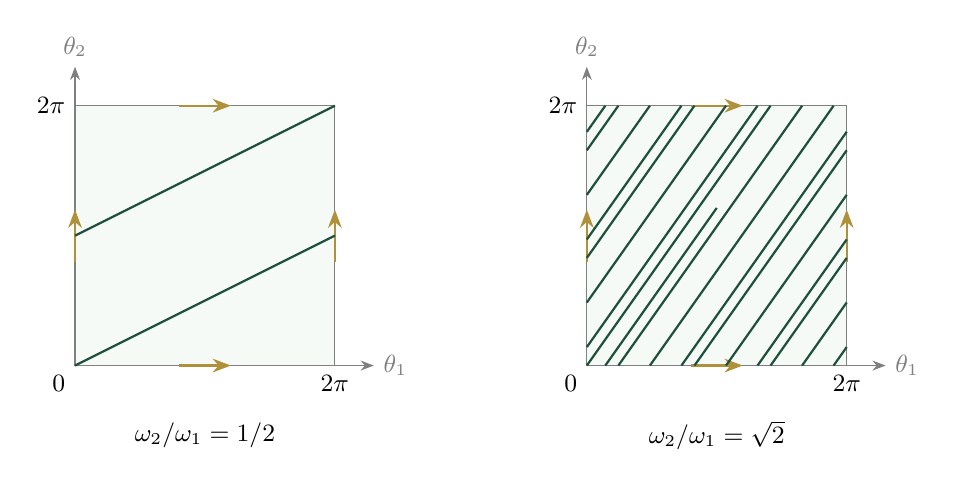
\begin{tikzpicture}[>=Stealth,font=\small]
\begin{scope}[shift={(0,0)},scale=3.3]

 \fill[GreenPale,opacity=.25] (0,0) rectangle(1,1);
 \draw[gray] (0,0) rectangle(1,1);
 \draw[->,gray] (0,0)--(1.15,0) node[right]{$\theta_1$};
 \draw[->,gray] (0,0)--(0,1.15) node[above]{$\theta_2$};
 \node[below left] at (0,0){$0$};\node[below] at (1,0){$2\pi$};\node[left] at (0,1){$2\pi$};
 \draw[GoldMain,->,thick] (.4,0)--(.6,0);\draw[GoldMain,->,thick] (.4,1)--(.6,1);
 \draw[GoldMain,->,thick] (0,.4)--(0,.6);\draw[GoldMain,->,thick] (1,.4)--(1,.6);
\draw[GreenMain,thick] (0.000000,0.000000)--(1.000000,0.500000);
\draw[GreenMain,thick] (0.000000,0.500000)--(1.000000,1.000000);
\node at (.5,-.27){$\omega_2/\omega_1=1/2$};
\end{scope}
\begin{scope}[shift={(6.5,0)},scale=3.3]

 \fill[GreenPale,opacity=.25] (0,0) rectangle(1,1);
 \draw[gray] (0,0) rectangle(1,1);
 \draw[->,gray] (0,0)--(1.15,0) node[right]{$\theta_1$};
 \draw[->,gray] (0,0)--(0,1.15) node[above]{$\theta_2$};
 \node[below left] at (0,0){$0$};\node[below] at (1,0){$2\pi$};\node[left] at (0,1){$2\pi$};
 \draw[GoldMain,->,thick] (.4,0)--(.6,0);\draw[GoldMain,->,thick] (.4,1)--(.6,1);
 \draw[GoldMain,->,thick] (0,.4)--(0,.6);\draw[GoldMain,->,thick] (1,.4)--(1,.6);
\draw[GreenMain,thick] (0.000000,0.000000)--(0.707107,1.000000);
\draw[GreenMain,thick] (0.707107,0.000000)--(1.000000,0.414214);
\draw[GreenMain,thick] (0.000000,0.414214)--(0.414214,1.000000);
\draw[GreenMain,thick] (0.414214,0.000000)--(1.000000,0.828427);
\draw[GreenMain,thick] (0.000000,0.828427)--(0.121320,1.000000);
\draw[GreenMain,thick] (0.121320,0.000000)--(0.828427,1.000000);
\draw[GreenMain,thick] (0.828427,0.000000)--(1.000000,0.242641);
\draw[GreenMain,thick] (0.000000,0.242641)--(0.535534,1.000000);
\draw[GreenMain,thick] (0.535534,0.000000)--(1.000000,0.656854);
\draw[GreenMain,thick] (0.000000,0.656854)--(0.242641,1.000000);
\draw[GreenMain,thick] (0.242641,0.000000)--(0.949747,1.000000);
\draw[GreenMain,thick] (0.949747,0.000000)--(1.000000,0.071068);
\draw[GreenMain,thick] (0.000000,0.071068)--(0.656854,1.000000);
\draw[GreenMain,thick] (0.656854,0.000000)--(1.000000,0.485281);
\draw[GreenMain,thick] (0.000000,0.485281)--(0.363961,1.000000);
\draw[GreenMain,thick] (0.363961,0.000000)--(1.000000,0.899495);
\draw[GreenMain,thick] (0.000000,0.899495)--(0.071068,1.000000);
\draw[GreenMain,thick] (0.071068,0.000000)--(0.500000,0.606602);
\node at (.5,-.27){$\omega_2/\omega_1=\sqrt2$};
\end{scope}
\end{tikzpicture}
\captionof{figure}{将环面沿经纬线展开为正方形；同向箭头标明需粘合的对边，右图只画有限轨道段。}
\label{fig:ode-tikz-torus-flow}
\end{minipage}
\end{center}

\section{均匀分布与高维推广}
\begin{definition}
圆上的序列 $\theta_n$ 称为均匀分布，若对每条弧 $J$，
$\#\{0\leq n<N:\theta_n\in J\}/N\to|J|/(2\pi)$。
连续环面流的均匀分布，是指落入每个坐标矩形的时间比例趋于该矩形的归一化体积。
\end{definition}
\begin{lemma}[三角多项式逼近]
环面上的连续函数可被三角多项式一致逼近。
\end{lemma}
\begin{proof}
圆上取 Fejér 核
\[
 K_N(s)=\frac1N\left|\sum_{j=0}^{N-1}e^{ijs}\right|^2.
\]
它非负、积分为 $2\pi$，是三角多项式；离开零点的固定邻域时，
$K_N(s)\leq[N\sin^2(s/2)]^{-1}$，积分质量趋于零。
卷积 $f*K_N/(2\pi)$ 与 $f$ 的差，
在零点附近由一致连续性控制，在远处由上述质量界控制，所以一致趋于零。
高维取各坐标核的乘积，重复同一估计即可。
\end{proof}
\begin{theorem}
无理圆周旋转序列均匀分布。
若 $\omega$ 有理独立，则环面线性流均匀分布，因而每条轨道稠密。
\end{theorem}
\begin{proof}
对非零整数 $k$，无理旋转的指数平均是有限等比和除以 $N$：
\[
 \frac1N\sum_{n=0}^{N-1}e^{ik(\theta+n\alpha)}\longrightarrow0,
\]
因为分母 $1-e^{ik\alpha}\ne0$ 而分子有界。
对高维连续流，若 $k\ne0$，则 $k\cdot\omega\ne0$，所以
\[
 \frac1T\int_0^Te^{ik\cdot(\theta_0+\omega t)}\,\dd t\longrightarrow0.
\]
常数项的平均为自身。于是对三角多项式，轨道平均等于空间平均的极限。
由一致逼近，把这一结论推广到所有连续函数。

弧或矩形的示性函数不连续，但其边界体积为零。
在边界宽度 $\delta$ 的小带内做分段线性过渡，构造上下连续函数夹住示性函数，
二者空间积分之差随 $\delta\to0$ 趋于零。
对上下函数先取时间平均再夹逼，得到所需频率公式。
任意非空开集包含正体积小矩形，因而轨道必与之相交，故稠密。
\end{proof}
例如 $\log_{10}2$ 无理（否则 $2^q=10^p$ 违反整数的唯一分解）。
所以 $2^n$ 的首位为 $d$ 的频率为
$\log_{10}(1+1/d)$；同样可以讨论任意给定的前若干位数字所占的比例。
稠密性表示序列与任一非空开弧相交；均匀分布还给出了序列各项落入每条弧的比例。

\setchapterimage{figure/Chapter11封面图.jpg}
\setchapterintro{本章从坐标图定义流形，再构造切空间、切丛和向量场。在坐标图中可应用前面建立的微分方程局部理论；紧性则使局部解拼接成全局相流。}
\chapter{流形上的微分方程}\label{chap:manifolds}

第~\ref{chap:arnold-geometry}~章中的坐标变换发生在 Euclidean 开集之间；环面运动又表明，一个相空间未必能由单张 Euclidean 坐标图覆盖。本章先建立换图、切空间和切丛，再把已有局部方程拼接为流形上的相流。

\section{坐标图与微分结构}
\begin{definition}
集合 $M$ 的一张 $n$ 维坐标图是双射 $\phi:W\to U$，其中 $W\subset M$、
$U\subset\R^n$ 为开集。
两图相容，是指重叠部分在各图中的像为开集，且过渡映射
$\phi_j\phi_i^{-1}$ 为光滑微分同胚。
相容且覆盖 $M$ 的坐标图族称图册。
两个图册若合并后仍相容，称为等价；等价类称光滑结构。
带光滑结构的集合，在下述分离与可数条件下称光滑流形。
\end{definition}
\begin{definition}
流形子集 $G$ 称开集，若每图中的 $\phi(G\cap W)$ 均开。
要求任意两不同点有不相交开邻域，称 Hausdorff 条件。
要求拓扑有可数个开集组成的基，称第二可数条件；这里“基”指任一开集都能写成这些开集的并。
对于局部 Euclidean 空间，这等价于存在可数坐标图册：每张图内的有理球给出可数基；
反向则用可数基选取包含在坐标域内的基元素，得到可数坐标子覆盖。
本章的流形均满足这两个条件，且无边界。
\end{definition}
由过渡映射相容性可知开集定义与图册选择无关。
若仅要求过渡映射为同胚，得到拓扑流形；要求 $C^r$ 或解析则得到相应类别。
定向图册要求换图映射的 Jacobi 行列式为正。


\begin{definition}[定向、闭流形与带边界流形]\label{def:orientation-boundary}
在 $n$ 维实向量空间中，两组有序基若换基行列式为正，就规定它们有相同定向。
在每个坐标域选择定向，且所有重叠处换图行列式为正，称给流形选定了定向；
能够这样选择时称可定向。
紧且无边界的流形称闭流形，这里的“闭”不只是说它在某个环境空间中是闭集。
允许坐标域是半空间 $\{x_n\geq0\}$ 中的相对开集，就得到带边界流形；
局部对应 $x_n=0$ 的点组成边界 $\partial M$。
边界的定向约定为：先写向外法向量，再写边界的有序切向基，应得到内部的正向基。
\end{definition}

\begin{example}[球面的两图]
单位球面 $S^n\subset\R^{n+1}$ 的南北极立体投影给出两图。
其过渡映射在非零点为 $x\mapsto x/|x|^2$，自身是逆，故光滑。
这两图覆盖整个球面，定义其光滑结构。
\end{example}
\begin{example}[射影空间]
$\mathbb{RP}^n$ 是 $\R^{n+1}$ 中过原点的直线的集合。
齐次坐标 $[x_0:\cdots:x_n]$ 把非零数倍坐标视为同一点。
在 $x_i\ne0$ 的区域，取其余 $n$ 个比值 $x_j/x_i$ 为坐标。
过渡关系均为分母非零的有理函数，所以给出 $n+1$ 张相容图。
\end{example}
环面用每个角坐标的两个开区间作图，其乘积给出有限图册。
这一构造不要求先把环面画在三维空间中。


\begin{definition}[覆盖映射]\label{def:covering-map}
连续满射 $\pi:\widetilde M\to M$ 称覆盖映射，若每个 $x\in M$ 有开邻域 $U$，
使 $\pi^{-1}(U)$ 是两两不交开集的并，且 $\pi$ 在每个这样的开集上都同胚到 $U$。
若每个点恰有 $k$ 个原像，称 $k$ 重覆盖。
例如 $\R\to\R/2\pi\Z$，$t\mapsto[t]$ 是覆盖；$S^n\to\mathbb{RP}^n$，$x\mapsto[x]$ 是双覆盖。
在半径足够小的球面片上，片与其对径片不交，各片都能唯一选取单位向量代表，故满足定义。
\end{definition}

\begin{definition}
子集 $K\subset M$ 紧，是指它的每个开覆盖均有有限子覆盖。
流形连通，是指它不能分成两个不相交非空开集。
连通分支的维数由任一坐标图的 Euclidean 维数定义。
\end{definition}
\begin{proposition}
若 $K$ 是有限个子集 $K_i$ 的并，各 $K_i$ 包含在一张图内且图像紧，则 $K$ 紧。
连通流形上的所有坐标图维数相同。
\end{proposition}
\begin{proof}
对任意开覆盖，利用坐标映射将各开集表示在相应的坐标域中，再由 $\phi_i(K_i)$ 的紧性选有限子覆盖，
再对有限个 $i$ 合并，得到 $K$ 的有限子覆盖。
换图映射的微分是两个坐标空间间的线性同构，故相交图具有相同维数。
固定一点，从它可由有限条相交坐标邻域链到达的点集是开集，其补集也开。
连通性使它为整个流形，所以所有图可沿链比较维数。
\end{proof}
球面以有限个有界小坐标片的紧闭子片覆盖，因而紧；射影空间亦可由单位球面
经连续映射 $x\mapsto[x]$ 得到，故紧。
局部图为局部道路连通空间，所以上述连通性也等价于有限图链连通和道路连通。


图~\ref{fig:ode-tikz-stereographic} 画出球面的一张坐标图；北极自身不在这张图的定义域内。
\begin{center}
\begin{minipage}{0.96\linewidth}
\centering
% TikZ mathematical illustration; compiled with the main document.
\begin{tikzpicture}[>=Stealth,font=\small,scale=2.15]
 \fill[GreenPale,opacity=.3] (0,0) circle(1);
 \draw[GreenMain,thick] (0,0) circle(1);
 \draw[->,gray] (-1.45,0)--(2.55,0) node[right]{投影平面};
 \draw[gray,dashed] (0,-1.15)--(0,1.25);
 \draw[GoldMain,thick] (0,1)--(2,0);
 \draw[GoldMain,->,thick] (.95,.525)--(1.35,.325);
 \fill (0,1) circle(1pt) node[above left]{$N$};
 \fill[GreenMain] (.8,.6) circle(1pt) node[above right]{$P$};
 \fill[GoldMain] (2,0) circle(1pt) node[below]{$q$};
 \node[below left] at (0,0){$0$};
\end{tikzpicture}
\captionof{figure}{立体投影的二维截面：从北极 $N$ 出发的直线将球面点 $P$ 映到平面点 $q$。}
\label{fig:ode-tikz-stereographic}
\end{minipage}
\end{center}

\section{光滑映射、子流形与例子}
\begin{definition}
$f:M\to N$ 光滑，是指其所有局部坐标表示 $\psi f\phi^{-1}$ 光滑。
光滑可逆且逆也光滑时称微分同胚。
光滑曲线是区间到流形的光滑映射，可有自交或零速度。
子集 $V\subset M$ 称 $k$ 维子流形，若在其每点附近有图使它成为
$\R^k\times\{0\}$ 与图域的交。
\end{definition}
\begin{proposition}[正则方程定义子流形]
若 $F:U\subset\R^N\to\R^{N-k}$ 光滑，且在 $F^{-1}(0)$ 上微分满秩，
则 $F^{-1}(0)$ 是 $k$ 维子流形。
\end{proposition}
\begin{proof}
在一点选取一个非零的 $(N-k)$ 阶子式，把其对应变量与其余 $k$ 个变量分开。
隐函数定理把前者写成后者的光滑函数。
以“前者减去该函数”和后者作坐标，零集恰成为坐标平面。
\end{proof}
下文将实正交群及特殊正交群分别记为 $O(n)$ 和 $SO(n)$。
\begin{example}[正交群]
把矩阵视为 $\R^{n^2}$ 的点，令 $F(Q)=Q^TQ-I$，其值在对称矩阵空间。
在正交矩阵处，$DF_Q(H)=Q^TH+H^TQ$。
任给对称矩阵 $S$，取 $H=QS/2$ 即得到 $S$，故满秩。
所以 $O(n)$ 是维数 $n(n-1)/2$ 的流形。
行列式的符号区分两个连通分支：$SO(n)$ 与一个反射乘 $SO(n)$。
用二维坐标平面旋转逐次消去一列的非对角元，可将任意 $SO(n)$ 元素连续连到恒等阵；
最后剩余对角的成对负号可用角度从零到 $\pi$ 的平面旋转消去。
因此这两个集合确实分别连通。
\end{example}
同样，$GL(n,\R)$ 也有两个分支。对可逆矩阵作极分解
$A=QP$，$P=(A^TA)^{1/2}>0$，路径 $(1-t)P+tI$ 始终正定，
把它变形到 $Q$，再用上面对正交群的分析即可。
取 $A^TA$ 的正定平方根，并令 $Q=AP^{-1}$，则
$Q^TQ=P^{-1}A^TAP^{-1}=I$，所以这也给出了所用极分解的具体构造。


\begin{definition}[浸入、嵌入与把手]\label{def:immersion-embedding}
光滑映射 $f:M\to N$ 的每点微分单射时称浸入；若它还单射，且作为 $M\to f(M)$ 的映射是到子空间拓扑的同胚，称光滑嵌入。
因此嵌入不仅要求参数化没有零速度，还要求没有不同点重合或全局拓扑不相容。
从两个曲面各去掉一个开圆盘，再沿边界圆粘合，得到它们的连通和。
球面与 $g$ 个环面的连通和称为带 $g$ 个把手的可定向曲面；$g$ 称亏格。
\end{definition}

\paragraph{拓扑预备结论。}
连通一维无边界流形微分同胚于圆或实线；闭连通可定向曲面微分同胚于带若干把手的球面。
Whitney 嵌入定理保证每个光滑 $n$ 维流形能嵌入充分高维的 Euclidean 空间。
这些分类与嵌入结果在本章中作为拓扑预备定理使用。
流形同胚不必微分同胚；同一拓扑球面上可能存在不同的光滑结构。

\section{切空间与切丛}
\begin{definition}
过 $x\in M$ 的两条光滑曲线，若在一张图中的初速度相同，称在 $x$ 相切。
等价类称 $x$ 处切向量，所有等价类组成 $T_xM$。
其线性运算由坐标中的速度向量定义。
\end{definition}
\begin{proposition}
相切与线性结构不依赖图的选择；$\dim T_xM=\dim M$。
光滑映射 $f$ 诱导线性映射
\[
 T_xf:T_xM\to T_{f(x)}N,
\]
且 $T(gf)=Tg\circ Tf$。
\end{proposition}
\begin{proof}
另一张图中的速度由换图映射的 Jacobi 矩阵作用于原速度得到，该矩阵可逆。
所以速度相等、加法和数乘在换图后保持。
每个坐标速度均可由一条小直线的逆图像实现，故切空间同构于 $\R^n$。
令 
\[
 T_xf[\gamma]=[f\gamma],
\]
链式法则同时证明良定义、线性和复合公式。
\end{proof}
\begin{definition}
不交并 
\[
 TM=\coprod_{x\in M}T_xM
\]
 称切丛的总空间。
投影 $p:TM\to M$ 把切向量送到附着点，$M$ 称底空间，$p^{-1}(x)$ 称纤维。
零截面 $i:M\to TM$ 将 $x$ 送到 $T_xM$ 的零向量。
\end{definition}
\begin{theorem}
$TM$ 有自然的 $2n$ 维光滑流形结构；其图坐标为 $(x,v)$，换图为
\[
 (x,v)\longmapsto(g(x),Dg(x)v).
\]
$p,i$ 及 $Tf:TM\to TN$ 都光滑，且 $pi=\operatorname{id}_M$。
\end{theorem}
\begin{proof}
换图公式来自速度的链式法则，光滑且逆由 $g^{-1}$ 给出。
复合过渡关系也由链式法则满足，所以给出图册。
在图中，投影为 $(x,v)\mapsto x$，零截面为 $x\mapsto(x,0)$，
切映射为 $(x,v)\mapsto(f(x),Df(x)v)$，因此均光滑，复合式也直接成立。
\end{proof}
对于 $C^r$ 流形，切丛的换图映射一般仅属于 $C^{r-1}$，因为其表达式含原换图映射的一阶导数。本章讨论 $C^\infty$ 流形。


\begin{definition}[向量丛、截面与标架]\label{def:vector-bundle}
秩 $k$ 的光滑向量丛包括总空间 $E$、底空间 $M$ 和光滑投影 $p:E\to M$，
每个纤维 $E_x=p^{-1}(x)$ 是 $k$ 维向量空间；在每点附近有
$p^{-1}(U)\simeq U\times\R^k$ 的光滑对应，且在每条纤维上是线性同构。
这样的对应称局部平凡化。光滑映射 $s:M\to E$ 满足 $p\circ s=\operatorname{id}$ 时称截面。
两个同底空间向量丛之间逐纤维线性的微分同胚称丛同构。
一组在每条纤维组成基的光滑截面称标架；只在一个开集上选取时称局部标架。
切丛的局部平凡化就是前面构造的 $(x,v)$ 坐标，因而满足这些条件。
\end{definition}
\begin{definition}[度量与梯度]\label{def:riemannian-gradient}
Riemann 度量是在各切空间上光滑选取的正定内积 $g_x$。
在局部坐标中它由正定对称矩阵 $(g_{ij}(x))$ 表示，
$|v|_g^2=\sum_{i,j}g_{ij}v_iv_j$。
函数 $f$ 的梯度由
\[
 g_x(\operatorname{grad}f(x),v)=df_x(v)\quad(v\in T_xM)
\]
唯一确定，坐标分量是 $(g_{ij})^{-1}Df^T$。
对于 Euclidean 子流形，使用环境内积在切空间上的限制。
单位切向量丛为 $T^1M=\{(x,v)\in TM:|v|_g=1\}$。
\end{definition}

\begin{definition}
若存在逐纤维线性的丛同构 $TM\simeq M\times\R^n$，称 $M$ 可平行化。
等价地，可在全流形选出 $n$ 个处处线性无关的光滑向量场。
\end{definition}
\begin{proof}[等价性的证明]
丛同构把 $\R^n$ 的标准基拉回，得到全局标架。
反之，给定标架，把 $(x,c_1,\ldots,c_n)$ 送到基向量的线性组合。
在局部图中这是光滑可逆矩阵作用，逆矩阵光滑，所以得到丛同构。
\end{proof}
Euclidean 开集与环面可平行化，后者取各角方向的速度场。

\begin{definition}[Möbius 带]
将 $[0,1]\times(-1,1)$ 中的 $(0,s)$ 与 $(1,-s)$ 识别，取商拓扑及由局部矩形诱导的光滑坐标，
所得曲面称开 Möbius 带。区间的中线拼成圆，横向坐标绕一周变号。
\end{definition}

Möbius 带不可平行化：沿中心圆走一周，横向基方向反转，换图映射的 Jacobi 行列式为负，
所以它不可定向；而全局标架会给出连续定向，矛盾。
球面 $S^2$ 不存在无零切向量场，将在指标和定理后证明。
对于任意维球面，可平行化性需要另行讨论。这里仅使用上述例子及后面由指标和定理得到的 $S^2$ 结论。

\section{几个相互微分同胚的三维流形}
\begin{definition}[四元数的共轭与范数]
四元数的标准基记为 $1,i,j,k$。对 $q=a+bi+cj+dk$，定义其共轭为
$\overline q=a-bi-cj-dk$。
范数由 $|q|^2=q\overline q$ 给出，纯虚四元数指实部为零的元素。
结合律及 $\overline{pq}=\overline q\,\overline p$ 给出
$|pq|^2=pq\overline q\,\overline p=|p|^2|q|^2$。
\end{definition}
\begin{proposition}
下列流形微分同胚：$SO(3)$、单位切向量丛 $T^1S^2$、$\mathbb{RP}^3$、
空间中固定一点的刚体的姿态空间，以及
\[
 \{z\in\C^3:z_1^2+z_2^2+z_3^2=0,\quad |z|^2=2\}.
\]
\end{proposition}
\begin{proof}
给 $(x,v)\in T^1S^2$，$|x|=|v|=1,x\perp v$，矩阵 $(x,v,x\times v)$ 属于 $SO(3)$。
取前两列是逆映射，故是微分同胚。刚体姿态由一组正向正交标架确定，
也与 $SO(3)$ 对应。
写 $z=x+iy$，复方程给出 $|x|^2=|y|^2,x\cdot y=0$，
范数条件给出二者均为 1，因而与同一个单位切向量模型对应。

最后用单位四元数 $q\in S^3$ 作用于纯虚四元数 $v\in\R^3$：
$v\mapsto qvq^{-1}$。乘法保持范数，所以得到旋转；
绕单位轴 $u$ 旋转角 $\theta$ 由 $q=\cos(\theta/2)+u\sin(\theta/2)$ 实现。
核恰为 $\{1,-1\}$，故诱导 $S^3/\{\pm1\}=\mathbb{RP}^3$ 到 $SO(3)$ 的双射。
其在单位元的微分为 $v\mapsto2u\times v$，从纯虚四元数到反对称矩阵空间是同构，
所以是局部微分同胚；结合双射得到全局微分同胚。
\end{proof}

\section{向量场与紧支撑相流}
\begin{definition}
流形上的向量场是光滑截面 $v:M\to TM$，满足 $pv=\operatorname{id}_M$。
积分曲线满足 $\gamma'(t)=v(\gamma(t))$。
若 $v$ 在某紧集外为零，称为紧支撑向量场；若其所有积分曲线均双向全局存在，称为完备。
\end{definition}
\begin{theorem}[紧支撑完备性]\label{thm:arnold-compact-flow}
紧支撑光滑向量场完备，并生成全局单参数微分同胚群。
特别地，紧流形上的每个光滑向量场都完备。
\end{theorem}
\begin{proof}
每点在一张坐标图内应用前文的存在唯一性与光滑依赖定理，
得到一个邻域及所有初值共用的正存在时间。
这里 $K=\operatorname{supp}v$，支撑按定义~\ref{def:support-test} 在流形拓扑中取闭包。用有限个这样的邻域覆盖紧集 $K$，取这些时间的一个正下界 $\delta$。
在 $K$ 外向量场为零，积分曲线恒定。
所以每个初值都至少有共同时间 $(-\delta,\delta)$ 的解。

在重叠坐标图里，局部解由唯一性一致，故拼接成流形上的解。
Hausdorff 条件保证“相同到某时刻”的闭性，排除在分叉的非 Hausdorff 空间中
局部唯一却整体分离的情况。
把小时间解反复复合，任意有限时间都可分成有限个长度小于 $\delta$ 的步长，
所以得到所有 $t\in\R$ 的解。
唯一性给出群性质，$\varphi^{-t}$ 为逆；每个有限复合由局部光滑映射组成，故光滑。
\end{proof}
\begin{corollary}
若 $M$ 紧，且 $v(t,x)$ 在 $\R\times M$ 光滑，则非自治方程的每个解也双向全局存在。
\end{corollary}
\begin{proof}
若最大存在区间有有限端点 $T$，在紧集 $[T-1,T+1]\times M$ 上用有限图覆盖，
得到共同正存在时间。取接近 $T$ 的一个已有时刻，其局部解可以跨越 $T$，矛盾。
正反向端点的证明相同。
\end{proof}

\section{线性方程的射影紧化}
\begin{proposition}
线性向量场 $x'=A(t)x$ 从 $\R^n$ 延伸为 $\mathbb{RP}^n$ 上的光滑含时向量场，
且无穷远超平面不变。
\end{proposition}
\begin{proof}
在无穷远附近取坐标 $y_1=1/x_1,y_k=x_k/x_1$（$k>1$）。
记 $B(y)=a_{11}+\sum_{j>1}a_{1j}y_j$，逐项求导得
\[
 y_1'=-y_1B(y),\qquad
 y_k'=a_{k1}+\sum_{j>1}a_{kj}y_j-y_kB(y).
\]
右端是 $y$ 的多项式，可以光滑延伸到 $y_1=0$。
那里第一分量为零，所以无穷远超平面不变。
其余图同理，重叠区域因与原场一致而相容。
\end{proof}
射影空间紧，故其含时解全局存在。
从仿射部分出发的轨道不可能在有限时间到达无穷远超平面：若到达，
由反向唯一性，它原本就应在这个不变超平面内。
因此原线性方程的解全局存在，这也是前面解的延拓定理的结论。

\setchapterimage{figure/Chapter12封面图.jpg}
\setchapterintro{首次积分把沿流不变的函数与一阶偏微分方程联系起来。本章依次研究线性、拟线性和一般非线性方程，并利用接触平面场研究隐式常微分方程。}
\chapter{特征线、偏微分方程与接触结构}\label{chap:characteristics}

第二章用全微分与首次积分求解平面方程，第~\ref{chap:arnold-geometry}~章给出非奇点附近的独立首次积分，而第~\ref{chap:manifolds}~章已定义切空间与子流形。本章据此研究向量场与初始曲面的横截性，并把隐式方程中的关系 $dy=p\,dx$ 表示为接触条件。

\section{线性方程的特征线与 Cauchy 问题}
\begin{definition}
在 $U\subset\R^n$ 上，一阶齐次线性方程为
\[
 L_a u=\sum_i a_i(x)\partial_i u=0.
\]
向量场 $a$ 的积分曲线称其特征线。
给定超曲面 $\Sigma$ 及函数 $g:\Sigma\to\R$，要求 $u|_\Sigma=g$，称为 Cauchy 问题。
若 $a(x_0)\notin T_{x_0}\Sigma$，称 $x_0$ 是非特征点。
\end{definition}
\begin{theorem}
在非特征点附近，$L_au=0,u|_\Sigma=g$ 存在唯一的局部光滑解。
它在每条特征线上保持初始值。
\end{theorem}
\begin{proof}
取 $\Sigma$ 的局部参数 $z$，以 $a$ 的流定义
\[
 F(s,z)=\varphi^s(\sigma(z)).
\]
横截性使 $DF(0,z_0)$ 可逆，故它是本章所需的流盒坐标。
在这些坐标中方程化为 $\partial_su=0$，初值在 $s=0$ 上。
因此唯一解为 
\[
 u(F(s,z))=g(\sigma(z)).
\]
这也直接证明了存在性、唯一性与光滑性。
\end{proof}
整体 Cauchy 问题未必可解：同一特征线若两次穿过初始超曲面，
在两个交点指定不同值便相互矛盾。
即使都在一个区域内，局部首次积分的表达式也不能不加检查地当成整体解。
例如 $xu_x-yu_y=0$ 的特征线保持 $xy$ 不变，但同一个 $xy$ 的不同连通分支
可以分别给定不同的光滑初始数据。

\begin{theorem}[非齐次特征线积分]
对 $L_au=b(x)$，在相同非特征假设下，唯一局部解满足
\[
 u(F(s,z))=g(\sigma(z))+\int_0^sb(F(\tau,z))\,\dd\tau.
\]
\end{theorem}
\begin{proof}
沿 $a$ 的轨道，链式法则给出 
\[
 \frac{\dd}{\dd s}u(F(s,z))=b(F(s,z)).
\]
对 $s$ 积分并使用初值即得表达式，反向求导则验证它满足方程。
\end{proof}

\section{拟线性方程与积分曲面}
\begin{definition}
一阶拟线性方程为
\[
 \sum_{i=1}^n a_i(x,u)\partial_i u=b(x,u).
\]
在 $(x,u)$ 空间中定义特征向量场 $A=(a,b)$，其积分曲线称特征线。
方向场若在曲面每点都属于其切空间，则该曲面称积分曲面。
\end{definition}
\begin{proposition}
函数 $u$ 解拟线性方程，当且仅当其图像为 $A$ 的积分曲面。
一个光滑曲面为积分曲面，当且仅当从其上出发的特征线局部仍留在曲面内。
\end{proposition}
\begin{proof}
图像的切向量具有形式 $(h,Du\,h)$，所以 $(a,b)$ 与图像相切恰好等价于
$Du\,a=b$。
若向量场相切，把它限制在曲面上，在曲面坐标中求解 ODE；
所得曲线也是环境空间中的解，由唯一性与环境解重合。
反过来，若曲线始终在曲面内，其初速度必属于切空间。
这里所有说法均在共同存在区间内使用。
\end{proof}

\begin{theorem}[拟线性 Cauchy 问题]
设在初始图像 $\{(\sigma(z),g(\sigma(z)))\}$ 上，
$a(x_0,g(x_0))\notin T_{x_0}\Sigma$。
则其附近存在唯一局部解，特征方程为
\[
 \dot x_i=a_i(x,u),\qquad \dot u=b(x,u).
\]
\end{theorem}
\begin{proof}
从初始图像发出特征线，得到 $(x(s,z),U(s,z))$。
在初始点，$x_s=a$ 与 $x_{z_j}=\sigma_{z_j}$ 线性无关，所以 $(s,z)\mapsto x$ 局部可逆。
由此特征线扫出的曲面是某个函数 $u(x)$ 的图像。
它由特征线组成，故由前一命题满足方程。
任何另一解图像也必须包含这些同初值特征线，唯一性使两者局部重合。
\end{proof}

\begin{example}[无相互作用介质与光滑解失效]
粒子作匀速运动，若初始速度是 $g(\xi)$，则
\[
 x=\xi+t g(\xi),\qquad u=g(\xi),\qquad u_t+uu_x=0.
\]
当 $1+tg'(\xi)\ne0$ 时可反解 $\xi$；且
\[
 u_x=g'(\xi)/(1+tg'(\xi)).
\]
若某处 $g'<0$，正时间可能出现梯度爆破。
取 $g(\xi)=-\arctan\xi$，首次退化发生在 $t=1,\xi=0$；
取 $g(\xi)=\arctan\xi$ 时，正时间内上述分母始终非零，故不发生这种交叉。
特征线相交后的多值表达式不再是原来的单值光滑解；以下只在投影局部可逆的区域内研究经典解。
\end{example}
若粒子受力 $F(x)$，则特征系统改为 $x'=u,u'=F(x)$，对应 PDE
$u_t+uu_x=F(x)$。
例如 $F=-x$、初值 $u(0,x)=0$，相流是旋转，解为
$u(t,x)=-x\tan t$，在 $|t|<\pi/2$ 成立。代入可得
\[
 u_t+uu_x=-x\sec^2t+x\tan^2t=-x.
\]


图~\ref{fig:ode-tikz-burgers-characteristics} 用线性初值展示投影退化：$x=\xi(1-t)$，在 $t=1$ 无法由 $x$ 唯一反解初始标号。
\begin{center}
\begin{minipage}{0.96\linewidth}
\centering
% TikZ mathematical illustration; compiled with the main document.
\begin{tikzpicture}[>=Stealth,font=\small,x=1.55cm,y=2.5cm]
 \draw[->,gray] (-2.25,0)--(2.3,0) node[right]{$x$};
 \draw[->,gray] (0,-.1)--(0,1.6) node[above]{$t$};
 \draw[GoldMain,dashed] (-2,1)--(2,1) node[right]{$t=1$};
 \foreach \xi in {-2,-1,-.5,.5,1,2}{
  \draw[GreenMain,thick] (\xi,0)--(0,1);
  \draw[GreenMain,dashed] (0,1)--({-.45*\xi},1.45);
  \draw[GreenMain,->,thick] ({.6*\xi},.4)--({.45*\xi},.55);
 }
 \fill[GoldMain] (0,1) circle(2pt);
 \node[fill=white,inner sep=2pt,anchor=east] at (-.25,1.45){投影退化};
 \node[below] at (-2,0){$\xi=-2$};\node[below] at (2,0){$\xi=2$};
\end{tikzpicture}
\captionof{figure}{初始速度 $g(\xi)=-\xi$ 的特征线在 $(t,x)=(1,0)$ 汇合；虚线表示交叉后的形式延长。}
\label{fig:ode-tikz-burgers-characteristics}
\end{minipage}
\end{center}


\subsection*{微分形式的坐标定义}
\begin{definition}[余向量与微分形式]\label{def:forms-coordinate}
记切空间的对偶空间为 $T_x^*M$，其中的元素称余向量。
在坐标 $z_1,\ldots,z_N$ 中，$dz_i(v)=v_i$，所以 $df=\sum_i(\partial_i f)dz_i$。
$k$ 形式是每点一个交替的 $k$ 重线性函数，且系数光滑；
“交替”指交换两个向量位置会变号。其局部表达为
\[
 \omega=\sum_{i_1<\cdots<i_k}a_{i_1\cdots i_k}(z)
 dz_{i_1}\wedge\cdots\wedge dz_{i_k}.
\]
这里的楔积规定
\[
 (dz_{i_1}\wedge\cdots\wedge dz_{i_k})(v_1,\ldots,v_k)
 =\det\bigl((v_b)_{i_a}\bigr)_{a,b=1}^k.
\]
通过线性展开定义一般楔积；相邻两个 $dz_i$ 交换变号，重复指标的乘积为零。
$0$ 形式就是函数。$1$ 形式 $\alpha$ 的核为
$\ker\alpha_x=\{v:\alpha_x(v)=0\}$。
\end{definition}
\begin{definition}[拉回、外微分与收缩]\label{def:exterior-pullback}
光滑映射 $h:M\to N$ 对形式的拉回定义为
\[
 (h^*\omega)_x(v_1,\ldots,v_k)
 =\omega_{h(x)}(Dh_xv_1,\ldots,Dh_xv_k).
\]
对 $\omega=\sum_Ia_I dz_I$，定义外微分
$d\omega=\sum_{I,j}(\partial_j a_I)dz_j\wedge dz_I$。
收缩定义为 $(\iota_X\omega)(v_2,\ldots,v_k)=\omega(X,v_2,\ldots,v_k)$。
\end{definition}
\begin{proposition}
上述定义在换坐标后相容，并满足
\[
 d^2=0,\qquad d(h^*\omega)=h^*(d\omega),\qquad
 d(\alpha\wedge\beta)=d\alpha\wedge\beta+(-1)^k\alpha\wedge d\beta
\]
（$\alpha$ 为 $k$ 形式）。
\end{proposition}
\begin{proof}
坐标变换时 $dh_i=\sum_j\partial_jh_i\,dz_j$，将其代入楔积，得到子式行列式形式的换元规则，
也就是拉回的定义。再次求外微分时，混合二阶偏导对指标对称，而楔积对指标反对称，
因此二阶项成对抵消，给出 $d^2=0$ 和 $d(h^*\omega)=h^*d\omega$。
最后一式由系数的乘积求导得到；将新产生的微分移过 $k$ 个前置因子，就出现 $(-1)^k$。
这些恒等式还说明外微分的坐标定义彼此一致。
\end{proof}
\begin{definition}[闭形式与恰当形式]\label{def:closed-exact-form}
$d\omega=0$ 时称 $\omega$ 闭；存在 $\beta$ 使 $\omega=d\beta$ 时称恰当。
由 $d^2=0$，恰当形式总是闭的。
在凸开集上，闭 $1$ 形式 $\alpha=\sum a_i dx_i$ 有势函数：平移使 $0$ 在域内后取
\[
 H(x)=\int_0^1\sum_i a_i(tx)x_i\,dt.
\]
对 $x_j$ 求导，使用 $\partial_ja_i=\partial_i a_j$，被积函数变为 $\partial_t[ta_j(tx)]$，
所以 $\partial_jH=a_j(x)$。这一结论将用于平面首次积分的构造。
\end{definition}

\section{隐式常微分方程的 1-jet 几何}
下面在包含自变量、函数值及一阶导数的空间中研究隐式方程。
\begin{definition}
两个函数在同一点 $t$ 的函数值及一阶导数相同时，规定它们在 $t$ 有相同的 1-jet。
其等价类因而由 $(t,x,p)$ 表示，其中 $x=x(t)$、$p=x'(t)$。
空间 $J^1=\{(t,x,p)\}$ 上，1-形式 $\alpha=\dd x-p\,\dd t$ 的核是二维接触平面。
隐式方程 $F(t,x,p)=0$ 定义曲面 $E$；一条解曲线提升为
$(t,x(t),x'(t))$，其切向量同时在 $TE$ 与 $\ker\alpha$ 内。
\end{definition}
\begin{proposition}
在光滑曲面 $E$ 上，若 $TE\ne\ker\alpha$，两平面相交成一维方向场。
可用切向量
\[
 X_F=F_p(\partial_t+p\partial_x)-(F_t+pF_x)\partial_p
\]
表示它。$F_p\ne0$ 的点称投影正则点，此处方程局部可写 $p=v(t,x)$。
\end{proposition}
\begin{proof}
代入计算得
\begin{align*}
 \alpha(X_F)&=pF_p-pF_p=0,\\
 dF(X_F)&=F_tF_p+F_xpF_p-F_p(F_t+pF_x)\\
 &=0.
\end{align*}
若 $X_F=0$，则 $F_p=F_t+pF_x=0$，这恰是光滑曲面切平面与接触平面重合的情形。
其余点的交线由非零 $X_F$ 张成。
$F_p\ne0$ 时隐函数定理把曲面写成 $p=v(t,x)$，投影局部微分同胚；
交线投影为 $dx/dt=v(t,x)$。
\end{proof}
当 $F_p=0$ 时投影非正则，但只要两平面不相同，曲面上方向场仍有定义。
非正则点的投影形成判别曲线；接触平面恰等于切平面的点则需另作奇点分析。
例如 $p^2=t$，以 $(p,x)$ 为曲面坐标，接触式成为
$\dd x=2p^2\,\dd p$，所以
\[
 t=p^2,\qquad x=C+\frac23p^3.
\]
投影在 $p=0$ 形成半三次尖点；两侧分别是 $x'=\sqrt t$ 和 $x'=-\sqrt t$ 的解。
因此，一个隐式微分方程可能包含若干不同的显式方程分支。


图~\ref{fig:ode-tikz-jet-cusp} 取积分常数 $C=0$，用同一参数 $p$ 将斜率分支与半三次尖点对应起来。
\begin{center}
\begin{minipage}{0.96\linewidth}
\centering
% TikZ mathematical illustration; compiled with the main document.
\begin{tikzpicture}[>=Stealth,font=\small]
\begin{scope}[x=1.55cm,y=1.15cm]
 \draw[->,gray] (-.2,0)--(2.1,0) node[right]{$t$};
 \draw[->,gray] (0,-1.55)--(0,1.6) node[above]{$p$};
 \draw[GreenMain,thick,domain=0:1.3,samples=55] plot ({\x*\x},\x);
 \draw[GoldMain,thick,domain=-1.3:0,samples=55] plot ({\x*\x},\x);
 \node[GreenMain] at (1,1.5){$p=\sqrt t$};\node[GoldMain] at (1,-1.5){$p=-\sqrt t$};
\end{scope}
\draw[->,thick] (3.8,0)--(5,0) node[midway,above]{$\pi$};
\begin{scope}[shift={(6,0)},x=1.55cm,y=1.15cm]
 \draw[->,gray] (-.2,0)--(2.1,0) node[right]{$t$};
 \draw[->,gray] (0,-1.7)--(0,1.8) node[above]{$x$};
 \draw[GreenMain,thick,domain=0:1.3,samples=55] plot ({\x*\x},{2*\x*\x*\x/3});
 \draw[GoldMain,thick,domain=-1.3:0,samples=55] plot ({\x*\x},{2*\x*\x*\x/3});
 \fill (0,0) circle(1.6pt);
 \node at (1,-2.05){$x^2=4t^3/9$};
\end{scope}
\end{tikzpicture}
\captionof{figure}{隐式方程 $p^2=t$ 的两支与积分曲线投影：$t=p^2$、$x=2p^3/3$。}
\label{fig:ode-tikz-jet-cusp}
\end{minipage}
\end{center}

\section{一般非线性方程的特征系统}
设未知函数 $u=u(x_1,\ldots,x_n)$。
\begin{definition}
在一点函数值及全部一阶偏导数相同的函数视为具有相同 1-jet。
这些等价类组成的空间有坐标 $(x,p,u)$，$p_i=\partial_i u$，维数为 $2n+1$。
函数的 1-图是 $(x,Du(x),u(x))$ 的像。
接触形式为 $\alpha=\dd u-\sum_i p_i\,\dd x_i$。
在 $2n+1$ 维空间上，若 $1$ 形式满足 $\alpha\wedge(d\alpha)^n\ne0$，
则其核称接触结构。这里 $(d\alpha)^n$ 指 $n$ 次楔积；
对所给 $\alpha$ 展开后得到非零常数倍的
$du\wedge dx_1\wedge dp_1\wedge\cdots\wedge dx_n\wedge dp_n$，故确实满足条件。
保持接触平面场的微分同胚称接触变换；等价地，其拉回满足 $h^*\alpha=a\alpha$，其中 $a$ 处处非零。
\end{definition}
\begin{theorem}[非线性特征方程]
设 $F(x,p,u)=0$ 且 $F_p\ne0$。其特征系统为
\[
 \begin{aligned}
 \dot x_i&=F_{p_i},\\
 \dot p_i&=-F_{x_i}-p_iF_u,\\
 \dot u&=\sum_i p_iF_{p_i}.
\end{aligned}
\]
特征线留在 $F=0$ 上，且每个 $C^2$ 解的 1-图局部由特征线组成。
\end{theorem}
\begin{proof}
对 $F$ 沿所给向量场 $X$ 求导，各项两两相消，得 $XF=0$，
因此初值在能量超曲面上的解留在其中。
若 $u$ 是 PDE 解，对恒等式 $F(x,Du(x),u(x))=0$ 关于 $x_i$ 求导，得
\[
 F_{x_i}+\sum_jF_{p_j}u_{x_ix_j}+F_u u_{x_i}=0.
\]
于是沿 $x'=F_p$ 的曲线，
\begin{align*}
 p_i'&=\sum_j u_{x_ix_j}F_{p_j}\\
 &=-F_{x_i}-p_iF_u,\\
 u'&=Du\,x'=p\cdot F_p.
\end{align*}
故 1-图上的曲线满足特征方程，并由唯一性与对应特征线重合。
\end{proof}
为研究特征方程的解对接触形式的影响，先给出相应的微分运算。
依照定义~\ref{def:forms-coordinate}--\ref{def:exterior-pullback}，对 $1$ 形式 $\alpha=\sum_j a_j(z)\,dz_j$ 有
\[
 d\alpha=\sum_{i,j}(\partial_i a_j)\,dz_i\wedge dz_j,
\]
其中楔积和收缩均按前面的具体规则计算。定义
\[
 \mathcal L_X\alpha=d(\alpha(X))+\iota_Xd\alpha.
\]
它等于沿 $X$ 的流拉回该形式后对时间求导的结果，这可在坐标中逐项用链式法则验证。
具体地，两种计算都给出第 $j$ 个系数
\[
 (\mathcal L_X\alpha)_j
 =\sum_iX_i\partial_i a_j+\sum_i a_i\partial_jX_i.
\]
前一项来自系数沿轨道变化，后一项来自流的微分作用于被代入的切向量，因而两种定义一致。

\begin{theorem}[非特征初始数据的局部构造]
设在初始超曲面 $\Sigma$ 给定 $u=g$，且能选择初始 $p$ 满足
$p|_{T\Sigma}=dg$、$F(x,p,g)=0$，同时 $F_p$ 横截于 $\Sigma$。
则其附近由特征线生成唯一局部解。
\end{theorem}
\begin{proof}
先用光滑底空间坐标把初始超曲面写成 $\Sigma=\{x_n=0\}$。
记其参数为 $z=(x_1,\ldots,x_{n-1})$，初值为 $g(z)$。
条件 $p|_{T\Sigma}=dg$ 确定 $p_i=g_{z_i}$（$i<n$）。
横截条件为 $F_{p_n}\ne0$，因此在已经选择的初始 $p_n$ 分支附近，
方程 $F(z,0,D_zg,p_n,g)=0$ 由隐函数定理唯一解出光滑 $p_n(z)$。
这里的唯一性均针对这一初始 jet 分支。

从初始 jet 参数化 $j(z)$ 出发，记特征流为 $\Phi^s$，并写
\[
 J(s,z)=\Phi^s(j(z))=(x(s,z),p(s,z),U(s,z)).
\]
在 $s=0$，$x_{z_i}$ 是初始超曲面的切向基，而 $x_s=F_p$ 横截该超曲面，
故 $(s,z)\mapsto x(s,z)$ 的 Jacobi 矩阵可逆。缩小邻域后，可将扫出的曲面
写成 $x\mapsto(x,p(x),U(x))$。还须证明 $p=DU$，这一步不由投影可逆自动得到。

首先 $\alpha(X)=0$，初始曲面上也有 $j^*\alpha=0$。
对 $\alpha=dU-\sum_ip_i\,dx_i$，坐标计算给出
\[
 \mathcal L_X\alpha=dF-F_u\alpha.
\]
由前一定理 $F(J(s,z))=0$，故 $J^*dF=0$。
设 $a_i(s,z)=\alpha(J_{z_i}(s,z))$，对 $s$ 求导便得
\[
 \partial_sa_i=-F_u(J(s,z))a_i,\qquad a_i(0,z)=0.
\]
这一齐次标量方程只有零解，所以 $\alpha$ 在所有 $J_{z_i}$ 上为零；
在 $J_s=X$ 上也为零。这些向量张成扫出曲面的切空间，因此 $J^*\alpha=0$。
改用 $x$ 参数后即为 $dU=\sum_ip_i\,dx_i$，也就是 $p=DU$。
再代入沿流保持的 $F=0$，得到所求 PDE 解及初始条件。

若另一局部解具有相同初值和所选初始 jet 分支，则其 1-图包含 $j(z)$。
前一定理说明该图由特征线组成，ODE 唯一性使其包含同样的 $J(s,z)$。
投影局部可逆，所以两个解在共同邻域相同，局部唯一性得证。
\end{proof}
上式的 Lie 导数可不依赖一般张量理论来检查：
$\alpha(X)=0$，且 $d\alpha=\sum_i dx_i\wedge dp_i$；
代入 $X$ 后得到
\begin{align*}
 \iota_Xd\alpha
 &=\sum_iF_{p_i}dp_i+\sum_i(F_{x_i}+p_iF_u)dx_i\\
 &=dF-F_u\alpha.
\end{align*}
接触平面上的 $d\alpha$ 决定超曲面 $F=0$ 的特征方向，
因此保持接触平面场的变换也保持特征方向。
将 $F$ 乘以非零函数 $h$ 时，在 $F=0$ 上 $X_{hF}=hX_F$，仅改变参数而不改变特征曲线。

\section{Hamilton--Jacobi 方程与距离函数}
\begin{definition}
未知函数值 $u$ 不显含的一阶方程 $H(x,Du)=0$，称为 Hamilton--Jacobi 方程。
其特征系统中 $F_u=0$，所以 $(x,p)$ 满足
$x'=H_p,p'=-H_x$，这正是已有 Hamilton 方程的形式。
\end{definition}

\begin{definition}[法空间与管状坐标]
对 Euclidean 空间中的子流形 $M$，法空间为切空间的正交补 $(T_qM)^\perp$。
一组光滑选取的正交单位法向量称局部单位法向标架。
由 Schmidt 正交化可在足够小的邻域内选取这样的标架；由于各次除法的分母不为零，所得向量随参数光滑变化。
将小法向量 $v\perp T_qM$ 送到 $q+v$，若在所考察区域为一一的光滑坐标变换，称这些坐标为管状坐标。
下面的距离结论在局部闭嵌入片附近讨论，并将邻域缩小到最近点唯一的范围。对于非闭子流形，一般不能取处处相同的邻域半径。
\end{definition}

\begin{proposition}
在光滑嵌入子流形的充分小管状邻域内，距离函数 $r$ 在子流形外光滑，满足
$|\nabla r|^2=1$。
\end{proposition}
\begin{proof}
局部参数化子流形为 $q(z)$，取光滑单位法向标架 $n_j(z)$。
映射 $\Psi(z,s)=q(z)+\sum_j s_jn_j(z)$ 在 $s=0$ 处微分可逆，
其列分别张成切空间与法空间，故在小邻域中是微分同胚。
缩小邻域后最近点唯一：距离平方关于 $z$ 的 Hessian 在 $s=0$ 是
$2Dq^TDq$，正定，因连续性在小邻域仍正定；远离该参数点的子流形部分由嵌入性排除。
因此 $r^2=\sum_j s_j^2$。

最近点条件使 $x-q(z)$ 正交于切空间。对 $r^2=|x-q(z(x))|^2$ 求微分，
含 $dq$ 的项因正交性消失，得到
\[
 \nabla(r^2)=2(x-q(z(x))).
\]
子流形外除以 $2r$，得 $\nabla r=(x-q)/r$，其长度为 1。
子流形上距离函数通常不可微，故必须排除该集合。
\end{proof}

\setchapterimage{figure/Chapter13封面图.jpg}
\setchapterintro{本章从向量转过的圈数开始，给出曲线指标、奇点指标及其和的严格定义与证明。映射度把二维论证推广到高维，也说明相空间的拓扑会限制微分方程可能具有的平衡点。}
\chapter{向量场的指标、映射度与 Euler 特征数}\label{chap:indices}

第六章已经用结点、鞍点和闭轨描述局部相图。本章先定义平面向量场沿闭曲线的指标，再利用第~\ref{chap:manifolds}~章的流形与定向概念讨论全局限制；涉及积分形式时采用第~\ref{chap:characteristics}~章的微分形式记号。

\section{曲线指标及形变不变性}


\begin{definition}[同伦与曲线积分]\label{def:homotopy-line-integral}
两映射 $f_0,f_1:X\to Y$ 间的同伦是连续映射 $F:[0,1]\times X\to Y$，
满足 $F(0,x)=f_0(x)$、$F(1,x)=f_1(x)$；光滑对象间的光滑同伦另要求 $F$ 光滑。
对分段 $C^1$ 曲线 $\gamma:[a,b]\to\R^N$ 及 $1$ 形式 $\alpha=\sum_j a_jdx_j$，定义
\[
 \int_\gamma\alpha=\int_a^b\sum_j a_j(\gamma(t))\gamma_j'(t)\,dt.
\]
它在保方向的分段光滑换参数下不变，反向时变号；这是普通定积分换元公式的直接结果。
曲线闭合时也记为 $\displaystyle\oint_\gamma\alpha$。
\end{definition}
\begin{definition}
设 $v=(P,Q)$ 在一条闭曲线 $\gamma$ 上不为零。沿曲线连续选择向量方向角 $\theta$，
定义指标为 
\[
 \operatorname{ind}_v\gamma=(\theta(1)-\theta(0))/(2\pi).
\]
方向角可在参数区间的有限个小段连续接续；闭合性使总角差是 $2\pi$ 的整数倍。
\end{definition}
\begin{proposition}
\[
 \operatorname{ind}_v\gamma=
 \frac1{2\pi}\oint_\gamma\frac{P\,\dd Q-Q\,\dd P}{P^2+Q^2}.
\]
它与方向角起点的选择无关；曲线不穿过零点的形变、或曲线上不产生零点的场的形变，
均不改变指标。曲线连接时指标相加，反向时变号。
\end{proposition}
\begin{proof}
局部写 $P=\rho\cos\theta,Q=\rho\sin\theta$，计算分子为 $\rho^2\dd\theta$，
积分等于总角差。不同起始角只差固定的 $2\pi$ 整数倍，角差不变。
对于连续形变，在参数区间的有限个小段上分别选取连续方向角，可知总角差连续变化；指标又是整数，故只能保持常值。
连接与反向的结论由积分可加性得到。
\end{proof}
例如把复数视为平面向量，$v(z)=z^m$ 在单位圆的指标是 $m$，
负整数 $m$ 时只在去心平面上定义，也得到负指标。

\begin{theorem}[边界指标与零点]
若简单闭曲线包围的闭盘区域内向量场处处不为零，则边界指标为零。
因此边界指标非零时内部必有零点。
\end{theorem}
\begin{proof}
把曲线在盘内连续缩到一点，整个过程中不遇零点，指标不变。
常值曲线的方向向量不转动，指标为零。
对于光滑盘，也可用下面的闭形式积分论证，不依赖具体收缩。
\end{proof}

\subsection*{定向积分与分片构造}
\begin{definition}[从属分片与形式的积分]\label{def:partition-integration}
有限开覆盖 $\{U_i\}$ 的光滑分片统一是非负光滑函数 $\rho_i$，满足
$\sum_i\rho_i=1$ 且 $\operatorname{supp}\rho_i\subset U_i$。
对紧流形，可在每点选较小坐标球，其闭包包含在一个 $U_i$ 内；有限个较小球覆盖全流形。
用例~\ref{ex:smooth-cutoff} 的凸起构造 $b_i$，使它在较小球为正、支撑在较大坐标球内。
于是 $\rho_i=b_i/\sum_jb_j$ 给出分片。
\end{definition}
在 $n$ 维定向坐标中，顶次形式为 $\omega=a(x)dx_1\wedge\cdots\wedge dx_n$。
若支撑在一张正向图中，定义 $\displaystyle\int_M\omega=\displaystyle\int a(x)dx$。
一般情形定义为 $\sum_i\displaystyle\int_M\rho_i\omega$。
重积分换元公式保证一张图的结果与正向坐标选择无关；对两组分片使用乘积 $\rho_i\sigma_j$，
便知总和也与分片选择无关。因此这确实是一个确定的积分。
\begin{proposition}[Stokes 公式]\label{prop:forms-stokes-calculus}
在紧定向带边界 $n$ 流形上，对光滑 $(n-1)$ 形式 $\beta$ 有
\[
 \int_M d\beta=\int_{\partial M}\beta.
\]
\end{proposition}
\begin{proof}
由刚构造的有限分片，$\beta=\sum_i\rho_i\beta$，而
$\sum_i d(\rho_i\beta)=d\beta$。因此只需证明支撑在一张图内的情形。
在内部图中，把各系数延零到 $\R^n$，写
\[
 \beta=\sum_{j=1}^n(-1)^{j-1}b_j(x)
 dx_1\wedge\cdots\wedge\widehat{dx_j}\wedge\cdots\wedge dx_n,
 \qquad d\beta=\sum_j\partial_jb_j\,dx_1\wedge\cdots\wedge dx_n.
\]
帽号表示省略该项。逐次积分和紧支撑使每个全轴导数积分为零，故内部图没有边界贡献。
在边界图中改在半空间积分，切向全轴导数仍积分为零；法向半轴导数的积分由微积分基本定理等于边界值。
按“向外法向在先”的边界定向，该边界值的符号正好是 $\displaystyle\int_{\partial M}\beta$ 的符号。
把有限各片相加即得结论。这一证明只使用重积分换元、累次积分及一元基本定理。
\end{proof}


\section{孤立零点与平面指标和}
\begin{definition}
若 $x_0$ 是孤立零点，取包围它且不含其他零点的小正向圆，
其曲线指标称 $x_0$ 的指标。
两个足够小圆可在无零环带内相互变形，故该定义与半径无关。
\end{definition}

\begin{lemma}[平面 Green 公式]\label{lem:green-from-calculus}
设 $D$ 是边界分段光滑的有界平面区域，$P,Q$ 在其邻域连续可微，边界按内部在左侧的方向定向。则
\[
 \oint_{\partial D}P\,dx+Q\,dy
 =\iint_D(\partial_xQ-\partial_yP)\,dx\,dy.
\]
允许有限个孔，孔的边界因而取顺时针方向。
\end{lemma}
\begin{proof}
先对 $D=\{a\leq x\leq b,\ f(x)\leq y\leq g(x)\}$，
逐条计算上下边界的 $P\,dx$ 积分，再用一元微积分基本定理，得
\[
 \oint_{\partial D}P\,dx
 =\int_a^b[P(x,f(x))-P(x,g(x))]dx
 =-\iint_D\partial_yP\,dx\,dy.
\]
对水平简单区域同理得到 $\displaystyle\oint Q\,dy=\displaystyle\iint\partial_xQ$。
一般情形可在每个光滑边界片附近旋转坐标，把边界写成函数图像，并用有限光滑分片将形式分到这些片和内部小块。
每一片用刚才的基本定理计算；相邻片的内部边界成对反向而抵消，留下外边界及孔边界。
所需分片的明确构造和对任意维的同一计算见前面的命题~\ref{prop:forms-stokes-calculus}。
有限个边界角点可先用半径趋于零的小圆切去；场在闭区域邻域有界，所添圆弧的积分趋于零，
所去小区域的面积积分也趋于零，再取极限即可。
\end{proof}

\begin{theorem}[平面指标和]\label{thm:arnold-indexsum-plane}
设闭盘型区域 $D$ 的边界 $S$ 上 $v\ne0$，内部只有有限个孤立零点 $x_j$。
则
\[
 \operatorname{ind}_v S=\sum_j\operatorname{ind}_v(x_j).
\]
\end{theorem}
\begin{proof}
从 $D$ 挖掉每个零点的小闭圆盘，得到 $D'$。
在其中定义
\[
 \omega=(P\,dQ-Q\,dP)/(P^2+Q^2).
\]
局部 $\omega=d\theta$，所以 $d\omega=0$。
Green 公式作用于带孔区域，给出
\[
 0=\int_{D'}d\omega=\int_S\omega-\sum_j\int_{S_j}\omega.
\]
内边界在 $D'$ 的边界定向下为顺时针，所以出现负号。
除以 $2\pi$ 即得结论。
\end{proof}
\begin{proposition}[非退化零点]
若 $v(x_0)=0$ 且 $A=Dv(x_0)$ 可逆，则
\[
 \operatorname{ind}_v(x_0)=\operatorname{sgn}\det A.
\]
所以平面结点、焦点、中心指标为 $+1$，鞍点为 $-1$。
\end{proposition}
\begin{proof}
平移使 $x_0=0$，写 $v(x)=Ax+o(|x|)$。
可逆性使 $|Ax|\geq c|x|$。
在小圆上，直线形变 $Ax+s(v(x)-Ax)$ 始终不为零，
所以局部指标等于线性场的指标。
可逆线性矩阵可在不改变行列式符号的条件下连续变形到恒等或反射：
极分解先去掉正定伸缩，再在正交群的连通分支内变形。
恒等场绕一圈转一圈，反射场反向转一圈，得到所述符号。
\end{proof}
在坐标反转时，绕小圆的正方向与计算向量角的正方向同时反转，故局部指标不变。
一般微分同胚在小邻域可连续地用其非退化线性部分替代；同样的两次定向变化相消，
所以孤立零点指标是流形上的坐标无关概念。


图~\ref{fig:ode-tikz-node-saddle-index} 中，沿虚圆正向走一周，左图的向量方向正转一周，右图反转一周。
\begin{center}
\begin{minipage}{0.96\linewidth}
\centering
% TikZ mathematical illustration; compiled with the main document.
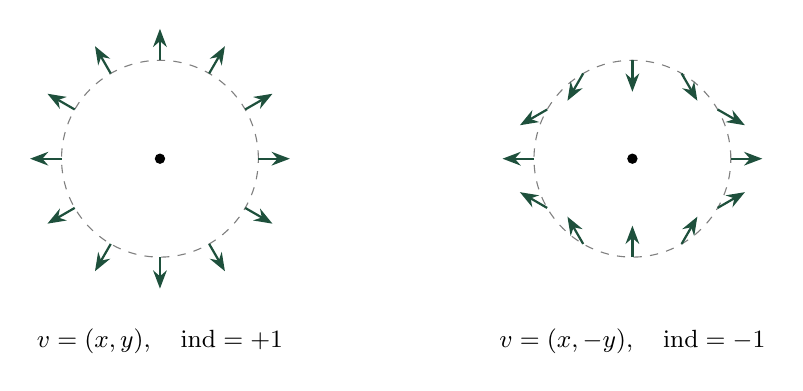
\begin{tikzpicture}[>=Stealth,font=\small]
\begin{scope}[shift={(0,0)},scale=1.25]
\draw[gray,dashed] (0,0) circle(1);\fill (0,0) circle(1.5pt);
\draw[->,GreenMain,thick] (1.00000,0.00000)--(1.32000,0.00000);
\draw[->,GreenMain,thick] (0.86603,0.50000)--(1.14315,0.66000);
\draw[->,GreenMain,thick] (0.50000,0.86603)--(0.66000,1.14315);
\draw[->,GreenMain,thick] (0.00000,1.00000)--(0.00000,1.32000);
\draw[->,GreenMain,thick] (-0.50000,0.86603)--(-0.66000,1.14315);
\draw[->,GreenMain,thick] (-0.86603,0.50000)--(-1.14315,0.66000);
\draw[->,GreenMain,thick] (-1.00000,0.00000)--(-1.32000,0.00000);
\draw[->,GreenMain,thick] (-0.86603,-0.50000)--(-1.14315,-0.66000);
\draw[->,GreenMain,thick] (-0.50000,-0.86603)--(-0.66000,-1.14315);
\draw[->,GreenMain,thick] (-0.00000,-1.00000)--(-0.00000,-1.32000);
\draw[->,GreenMain,thick] (0.50000,-0.86603)--(0.66000,-1.14315);
\draw[->,GreenMain,thick] (0.86603,-0.50000)--(1.14315,-0.66000);
\node at (0,-1.85){$v=(x,y),\quad\operatorname{ind}=+1$};
\end{scope}
\begin{scope}[shift={(6,0)},scale=1.25]
\draw[gray,dashed] (0,0) circle(1);\fill (0,0) circle(1.5pt);
\draw[->,GreenMain,thick] (1.00000,0.00000)--(1.32000,0.00000);
\draw[->,GreenMain,thick] (0.86603,0.50000)--(1.14315,0.34000);
\draw[->,GreenMain,thick] (0.50000,0.86603)--(0.66000,0.58890);
\draw[->,GreenMain,thick] (0.00000,1.00000)--(0.00000,0.68000);
\draw[->,GreenMain,thick] (-0.50000,0.86603)--(-0.66000,0.58890);
\draw[->,GreenMain,thick] (-0.86603,0.50000)--(-1.14315,0.34000);
\draw[->,GreenMain,thick] (-1.00000,0.00000)--(-1.32000,0.00000);
\draw[->,GreenMain,thick] (-0.86603,-0.50000)--(-1.14315,-0.34000);
\draw[->,GreenMain,thick] (-0.50000,-0.86603)--(-0.66000,-0.58890);
\draw[->,GreenMain,thick] (-0.00000,-1.00000)--(-0.00000,-0.68000);
\draw[->,GreenMain,thick] (0.50000,-0.86603)--(0.66000,-0.58890);
\draw[->,GreenMain,thick] (0.86603,-0.50000)--(1.14315,-0.34000);
\node at (0,-1.85){$v=(x,-y),\quad\operatorname{ind}=-1$};
\end{scope}
\end{tikzpicture}
\captionof{figure}{结点与鞍点的指标。虚圆是计算指标的边界，箭头表示边界各点的场向量。}
\label{fig:ode-tikz-node-saddle-index}
\end{minipage}
\end{center}

\section{指标的应用}
\begin{theorem}[代数基本定理的指标证明]
非常数复多项式至少有一个复根。
\end{theorem}
\begin{proof}
设 $p(z)=z^n+a_1z^{n-1}+\cdots+a_n$。
取 $R>1+\sum|a_j|$，在 $|z|=R$ 上，
$|z^n|>\sum|a_jz^{n-j}|$。
所以 $z^n+s\sum a_jz^{n-j}$（$0\leq s\leq1$）在圆上无零点。
其指标与 $z^n$ 相同，等于 $n\ne0$。
由边界指标定理，$p$ 在内部有零点。
进一步用局部因子 $(z-z_j)^{m_j}$ 和指标和公式，得到根数按重数等于边界绕数。
\end{proof}
\begin{theorem}[圆盘不动点]
闭圆盘到自身的每个光滑映射 $f$ 有不动点。
\end{theorem}
\begin{proof}
缩放为单位盘，假设没有不动点，则 $v(x)=f(x)-x$ 在闭盘处处不为零。
在边界 $|x|=1$，形变 $v_s=sf(x)-x$ 在 $s<1$ 时不为零，因为 $|sf(x)|<1$；
$s=1$ 时由假设也不为零。
所以边界指标与 $-x$ 相同，为 1，与无零点时指标为零矛盾。
\end{proof}
该结论与压缩映射定理不同：它不要求压缩，却只保证存在、不保证唯一。
连续映射的情形可以由一致光滑逼近和紧性推出。

\paragraph{半平面根数与稳定性。}
设实多项式 $p$ 在虚轴无根，次数为 $n$。
沿左半圆边界，先从 $-iR$ 沿虚轴到 $iR$，再沿左大半圆返回，
总像曲线的绕数等于左半平面根数 $n_-$。
大半圆部分在 $R\to\infty$ 时贡献 $n/2$ 圈，
所以若 $\nu$ 为虚轴像 $p(it)$（$t:-\infty\to\infty$）的连续总角增除以 $2\pi$，则
$n_-=\nu+n/2$。
这是原有 Routh--Hurwitz 问题的几何表示；$\nu$ 本身不必为整数，
但与半圆贡献合并后是整数。

\section{球面上的指标和}
\begin{theorem}
球面 $S^2$ 上只有孤立零点的光滑切向量场，其零点指标之和为 2。
\end{theorem}
\begin{proof}
若场不恒为零，可选一个非零点 $N$ 作北极；恒零场不符合只有孤立零点的假设。
零点集是紧球面上的闭集。由于每个零点孤立，紧性保证零点总数有限。
以南图坐标 $z$ 表示 $S^2\setminus\{N\}$，将所有零点包含在充分大的圆盘中。
平面指标和定理把所求总和化为大圆 $z=Re^{i\theta}$ 上向量分量的绕数。

在北极附近取另一坐标 $w=g(z)=z/|z|^2$，两图过渡反转平面定向。
记场在南、北图中的复数分量分别为 $u(z),v(w)$，则 $v(g(z))=Dg(z)u(z)$。
若 $z=Re^{i\theta}$，直接对反演求导，得到
\[
 Dg(z)\zeta=-R^{-2}e^{2i\theta}\overline\zeta,
 \qquad
 v(g(z))=-R^{-2}e^{2i\theta}\overline{u(z)}.
\]
这里复数共轭正是反射，正因子 $R^{-2}$ 不影响方向。
北图中 $N$ 附近场无零点，故其在小圆盘上的归一化方向连续延伸到盘内，
边界绕数为零。无论选择小圆的哪一方向，这个绕数都仍为零。
沿 $\theta:0\to2\pi$ 对上式取方向角增量，得到
\[
 0=2-\operatorname{wind}_{|z|=R}u.
\]
其中 $e^{2i\theta}$ 贡献两圈，复共轭使 $u$ 的绕数变号，负号只增加常角 $\pi$。
因此南图大圆上场的绕数为 2，也就是全部零点指标之和。
上述等式中，复共轭已计入换图时的定向反转，故由角度增量得到所需的指标。
\end{proof}
\begin{corollary}[毛球结论]
$S^2$ 上每个连续切向量场有零点，因此 $S^2$ 不可平行化。
\end{corollary}
\begin{proof}
若存在光滑无零场，零点指标和为零，与定理矛盾。
连续无零场因紧性有正的长度下界，用局部光滑逼近和有限分片统一拼接，
可得到仍无零的光滑场，故也不可能。
平行化会提供处处非零的基向量场，因此也被排除。
\end{proof}


\section{映射度的定义与计算}
下文流形紧、无边界且光滑；计算映射度时另要求同维、定向，目标连通。
\begin{definition}
$f:M^n\to N^n$ 在 $x$ 为正则，是指 $D f_x$ 可逆。
若 $f^{-1}(y)$ 的所有点都正则，称 $y$ 为正则值；空原像也允许。
正则点的局部度数为 $\deg_x f=+1$ 或 $-1$，由微分是否保持定向决定。
\end{definition}

\begin{definition}[零测集的覆盖意义]
集合 $Z\subset\R^n$ 称零测集，是指任给 $\varepsilon>0$，均可用可数个开长方体覆盖它，
且这些长方体体积之和小于 $\varepsilon$。
可数个零测集的并仍零测：对第 $j$ 个集合使用总体积小于 $\varepsilon2^{-j}$ 的覆盖，再合并。
以下只用这一覆盖性质，不预设一般 Lebesgue 积分。
流形上的零测集按可数坐标图内的像判断；紧坐标块上光滑换图为 Lipschitz，
长方体覆盖的体积估计因而保证该性质与图无关。
临界点是微分不可逆的点，临界值是临界点的像。
\end{definition}

\begin{lemma}[同维情形的正则值]
$C^1$ 映射的临界值集测度为零。紧流形映射在正则值上的原像有限。
\end{lemma}
\begin{proof}
后一结论先由逆函数定理知原像点孤立，再由紧性得有限。
对前一结论，只需在有限或可数个有界坐标块上证明。
把坐标块分成边长 $h$ 的小立方体。
若小块中含临界点 $x$，则 $Df_x$ 把立方体压到至少一个方向为零的平行六面体；
由导数的一致连续性，整个小块的像包含在其 $o(h)$ 邻域内。
导数有界，所以其像体积不超过 $C\varepsilon h^n$，其中当 $h$ 充分小时 $\varepsilon$ 任意小。
块数至多 $C'h^{-n}$，所以临界点集之像的外测度不超过 $CC'\varepsilon$。
令 $\varepsilon\to0$，并对可数坐标块求并，得测度零。
\end{proof}
\begin{definition}[顶次形式]
同伦采用定义~\ref{def:homotopy-line-integral}，这里要求它光滑。
在 $n$ 维定向坐标中，形如 $a(x)\,dx_1\wedge\cdots\wedge dx_n$ 的微分形式称为顶次形式；可写成 $d\beta$ 的形式称为恰当形式。
\end{definition}

下面使用前面已经定义的形式积分与命题~\ref{prop:forms-stokes-calculus}，将局部 Jacobian 符号与整体整数联系起来。


\begin{theorem}[度数不依赖正则值]
\[
 \deg f:=\sum_{x\in f^{-1}(y)}\deg_x f
\]
与正则值 $y$ 的选择无关，并在光滑同伦下不变。
\end{theorem}
\begin{proof}
给出该结论常用的积分论证。先使用如下顶次形式事实：
在连通定向闭 $n$ 流形上，积分相同的两个光滑 $n$ 形式之差是一个恰当形式。
它可用分片统一局部证明：在 $\R^n$，积分零的紧支撑函数 $h(x)$，
选积分为 1 的一维紧支撑函数 $\rho(x_1)$，令
$g(x')=\displaystyle\int h(s,x')\,ds$。
则 $h-\rho g$ 关于 $x_1$ 的原函数仍紧支撑；余项 $\rho g$ 对维数归纳，
因为 $\displaystyle\int g=0$。这证明积分零的紧支撑顶次形式恰当。
在流形上把形式分到坐标球，再沿相交坐标球链把每块的积分转移到同一小球；
相邻两块总积分为零的差由刚证的局部结论消去，最后仍是一个总积分零的小球内形式。
分片统一可由有限坐标覆盖、坐标内光滑非负凸起函数以及除以它们的正和构造。

选支撑在正则值 $y$ 的小邻域内且积分为 1 的顶次形式 $\eta_y$。
紧性与逆函数定理使其原像分成有限个微分同胚片，换元公式给出
\[
 \int_M f^*\eta_y=\sum_{x\in f^{-1}(y)}\operatorname{sgn}\det Df_x.
\]
另一个正则值的形式与它差 $d\beta$，Stokes 公式使
$\displaystyle\int_M f^*d\beta=0$，所以总和相同。
若 $F:[0,1]\times M\to N$ 为光滑同伦，顶次形式 $\eta$ 满足 $d\eta=0$，
在柱体上用 Stokes 公式得到
\[
 \begin{aligned}
 \int_MF_1^*\eta-\int_MF_0^*\eta
 &=\int_{[0,1]\times M}dF^*\eta\\
 &=0.
\end{aligned}
\]
因此度数同伦不变。
\end{proof}
\begin{proposition}
圆映射 $z\mapsto z^m$ 的度数为 $m$；
球面上的归一化线性映射 $x\mapsto Ax/|Ax|$ 的度数为 $\operatorname{sgn}\det A$；
$S^{n-1}$ 的对径映射度数为 $(-1)^n$。
\end{proposition}
\begin{proof}
第一个映射在非零 $m$ 时每个正则值有 $|m|$ 个原像，各局部符号为 $\operatorname{sgn}m$；
$m=0$ 为常值映射，选像外正则值得零。
第二个映射可用极分解在保持非退化条件下变形为正交映射，
后者在球面切空间的定向符号与环境空间行列式符号相同，因为径向方向同时保持向外。
最后取 $A=-I$ 即得 $(-1)^n$。
\end{proof}

\section{高维奇点指标与 Euler 特征数}
\begin{definition}
向量场在 $\R^n$ 中的孤立零点 $x_0$ 的指标，是小球面映射
$x\mapsto v(x)/|v(x)|\in S^{n-1}$ 的度数。
当 $n=2$，它与前面曲线绕数定义一致。
\end{definition}
\begin{proposition}
非退化零点的指标为 $\operatorname{sgn}\det Dv(x_0)$。
\end{proposition}
\begin{proof}
在小球面上用 $v(x)=A(x-x_0)+o(|x-x_0|)$ 直线形变到线性场，
可逆性保证整个形变无零点。归一化后度数不变，应用前一命题即得。
\end{proof}


\begin{definition}[有限三角剖分与 Euler 特征数]\label{def:euler-characteristic}
$k+1$ 个点 $v_0,\ldots,v_k$ 仿射无关，是指 $v_1-v_0,\ldots,v_k-v_0$ 线性无关。它们的凸包称 $k$ 单纯形，形如
$\{\sum_{j=0}^kt_jv_j:t_j\geq0,\ \sum_jt_j=1\}$；部分顶点的凸包称面。
有限个单纯形按公共面粘合，且每两单纯形相交为空或共同的面，得到有限单纯复形。
它到 $M$ 的一个同胚称 $M$ 的有限三角剖分。
若其中 $k$ 维单纯形有 $c_k$ 个，则
\[
 \chi(M)=\sum_k(-1)^kc_k
\]
称 Euler 特征数；对于曲面即顶点数减边数加面数。
同样可用有限胞腔分解计数：$k$ 维胞腔的内部是一份开 $k$ 球，边界粘到较低维部分。
这一整数对所选分解的不变性以及与向量场指标和的相等性，是下面全局指标和定理的内容。
\end{definition}

\paragraph{指标和的全局结论。}
Poincaré--Hopf 指标和定理断言：闭流形上孤立零点向量场的指标和与场无关，
等于流形的 Euler 特征数 $\chi(M)$。一般闭流形上的结论在这里作为拓扑预备定理使用；平面和二维球面的情形已在前面证明。

\begin{proposition}[球面、射影空间和环面]
在上述指标和定理下，
\[
 \chi(S^n)=1+(-1)^n,\qquad
 \chi(\mathbb{RP}^n)=\frac{1+(-1)^n}{2},\qquad
 \chi(\mathbb T^n)=0\quad(n\geq1).
\]
\end{proposition}
\begin{proof}
在球面取高度函数 $x_0$ 的梯度场，仅有南北两极为零点。
南极局部为正定线性场，指标 $+1$；北极为负定，指标 $(-1)^n$，故得第一式。
对双覆盖 $\pi:S^n\to\mathbb{RP}^n$，向量场的提升具体定义为
$\widetilde v(x)=(D\pi_x)^{-1}v(\pi(x))$。
各覆盖片上 $\pi$ 为局部微分同胚，故这个定义光滑且与取片无关；每个零点有两个原像且指标相同，
所以指标和乘以 2，得第二式。
环面上取恒定非零角速度场，无零点，指标和为零。
\end{proof}
因此偶维球面上每个光滑切向量场必有零点。
奇维球面 $S^{2m-1}\subset\C^m$ 上，$v(z)=iz$ 处处非零且与球面相切，
因为 $\operatorname{Re}\langle z,iz\rangle=0$，这与奇维 Euler 特征为零相符。

\noindent
这里临界点指 $df=0$ 的点；非退化指该点坐标 Hessian 矩阵可逆。
在临界点换坐标时 Hessian 作可逆合同变换，故此条件不依赖坐标。
梯度按定义~\ref{def:riemannian-gradient} 选定任一光滑正定度量；
其线性化实际是 $g^{-1}\operatorname{Hess}f$，由于 $\det g>0$，行列式符号与 Hessian 相同。
\medskip

\begin{proposition}[曲面上的临界点计数]
闭曲面上的光滑函数若临界点均非退化，记极小、鞍、极大点数为 $m_0,m_1,m_2$，则
\[
 m_0-m_1+m_2=\chi(M).
\]
对有 $g$ 个把手的可定向闭曲面，$\chi=2-2g$。
\end{proposition}
\begin{proof}



取上述梯度场，故局部指标等于 Hessian 的行列式符号：
极值为 $+1$，鞍点为 $-1$。应用指标和定理即得计数式。
带 $g$ 个把手的曲面有一个顶点、$2g$ 条边及一个面的标准多边形粘合表示，
故其胞腔 Euler 数为 $1-2g+1=2-2g$。
对球面的多面体分解，用连通平面图删除非树边，每删一边同时合并两个面，
$V-E+F$ 不变。最终一棵树有 $E=V-1$ 且只有一个面，故 $V-E+F=2$。
\end{proof}
对于有边界曲面，还须规定边界上的条件或计入边界指标，不能直接应用上述闭曲面公式。

\setchapterimage{figure/Chapter14封面图.jpg}
\setchapterintro{把已有的参数依赖、首次积分和相图方法用于具体问题。本章讨论中心力、相邻轨道、光线、退化一维场、种群系统及小扩散稳态。}
\chapter{几何方法的应用与若干进阶问题}\label{chap:applications}

本章的力学与光学例子分别使用常系数线性化、首次积分、Hamilton 方程以及下文给出定义的变分法；广义种群系统还会同时用到第六章的 Dulac 判据和第~\ref{chap:indices}~章的指标。最后对扩散方程的光滑解讨论其长期行为，解的存在性另作假设。

\section{中心力与相邻轨道的相对运动}
\begin{definition}
力场 $F(r)=a(|r|)r$ 称为中心力场。二维的面积速度为
$\frac12(r_1\dot r_2-r_2\dot r_1)$，三维的角动量为 $r\times\dot r$
（这里质量取 1）。
\end{definition}
\begin{proposition}
中心力下角动量守恒，二维面积速度守恒。Hamilton 系统中若 $H$ 不含某个坐标 $q_i$，
其共轭动量 $p_i$ 是首次积分。
\end{proposition}
\begin{proof}
\[
 \begin{aligned}
 \frac{\dd}{\dd t}(r\times\dot r)
 &=\dot r\times\dot r+r\times\ddot r\\
 &=r\times a(|r|)r\\
 &=0.
\end{aligned}
\]
二维行列式的求导相同，得到面积速度守恒。
Hamilton 方程给出 $\dot p_i=-\partial H/\partial q_i=0$，所以动量不变。
\end{proof}
面积速度守恒对任意中心力都成立，不能单凭 Kepler 第二定律推出反平方引力。
反平方尺度律还需周期与尺度的信息。

\begin{example}[空间站抛出物体]
以空间站的圆轨道半径、角速度作单位，在随站转动的坐标中，
记 $x$ 为向外径向位移，$y$ 为沿运动方向位移。
引力的圆轨道线性化与旋转坐标的加速度项给出
\[
 x''-2y'-3x=0,\qquad y''+2x'=0.
\]
确实，令 $J=\left(\begin{smallmatrix}0&-1\\1&0\end{smallmatrix}\right)$ 为旋转 $\pi/2$ 的矩阵，惯性加速度的局部形式为 $r''+2Jr'-r$，
而反平方引力在圆轨道点的导数在径向为 $+2$、切向为 $-1$；
两边相减便得到上述系数。
\end{example}
\begin{proposition}
初始相对位置为零、初始径向速度为 $v$、切向速度为零时，线性近似解为
\[
 x=v\sin t,\qquad y=2v(\cos t-1).
\]
它是半轴 $|v|,2|v|$、中心 $(0,-2v)$ 的椭圆，以一个轨道周期闭合。
\end{proposition}
\begin{proof}
第二式积分得 $y'+2x=0$；代入第一式得 $x''+x=0$。
由 $x(0)=0,x'(0)=v$ 得 $x=v\sin t$，再积分 $y'=-2v\sin t$ 得 $y$。
消去参数即得椭圆。
前文的参数可微依赖定理说明在固定有界时间内，真实解与该一阶近似之差为 $O(v^2)$。
这并不保证真实相对轨道严格闭合，也不保证无限时间误差仍是 $O(v^2)$。
\end{proof}


图~\ref{fig:ode-tikz-hill-ellipse} 取 $v=1$，标出空间站所在的相对原点及相对轨道的中心。
\begin{center}
\begin{minipage}{0.96\linewidth}
\centering
% TikZ mathematical illustration; compiled with the main document.
\begin{tikzpicture}[>=Stealth,font=\small,x=1.25cm,y=.85cm]
 \draw[->,gray] (-1.8,0)--(2.1,0) node[right]{$x$（径向）};
 \draw[->,gray] (0,-4.6)--(0,.8) node[above]{$y$（切向）};
 \draw[GreenMain,thick,domain=0:360,samples=100,variable=\t] plot ({sin(\t)},{2*(cos(\t)-1)});
 \draw[GreenMain,->,thick,domain=30:50,samples=12,variable=\t] plot ({sin(\t)},{2*(cos(\t)-1)});
 \draw[GreenMain,->,thick,domain=210:230,samples=12,variable=\t] plot ({sin(\t)},{2*(cos(\t)-1)});
 \draw[GoldMain,dashed] (-1,-2)--(1,-2);
 \fill[GoldMain] (0,-2) circle(1.7pt) node[above left]{$(0,-2)$};
 \fill (0,0) circle(1.7pt) node[above left]{空间站};
 \node at (3.1,-1.5){$x=\sin t$};\node at (3.1,-2.3){$y=2(\cos t-1)$};
\end{tikzpicture}
\captionof{figure}{初始径向速度为 $v>0$ 的线性相对轨道：椭圆中心在 $(0,-2v)$，并非空间站位置。}
\label{fig:ode-tikz-hill-ellipse}
\end{minipage}
\end{center}

\section{分层介质中的光线与 Clairaut 守恒量}

\begin{definition}[泛函、变分与驻曲线]\label{def:variation-functional}
把一条函数或曲线送到一个实数的规则称泛函。例如
\[
 \mathcal I[y]=\int_a^b L(x,y(x),y'(x))\,dx.
\]
固定端点，取光滑 $\eta$ 满足 $\eta(a)=\eta(b)=0$，将 $y$ 换成 $y+s\eta$，称作变分。
若对每个这样的 $\eta$，$\left.\frac d{ds}\mathcal I[y+s\eta]\right|_{s=0}=0$，称 $y$ 为驻曲线。
驻曲线不一定使泛函取最小值。
\end{definition}
\begin{lemma}[Euler--Lagrange 方程]\label{lem:euler-lagrange-elementary}
若 $L$ 足够光滑，$C^2$ 驻曲线满足
\[
 \frac d{dx}L_{y'}=L_y.
\]
\end{lemma}
\begin{proof}
在有限区间上微分积分，再分部积分，得到
\[
 0=\int_a^b(L_y\eta+L_{y'}\eta')dx
 =\int_a^b\left(L_y-\frac d{dx}L_{y'}\right)\eta\,dx.
\]
括号内若在一点严格为正，由连续性在一个小区间保持正；取支撑在其中的非负非零凸起函数作 $\eta$，积分便严格为正，矛盾。
负值同理排除，故括号处处为零。对向量曲线逐个分量作变分，得到相应方程组。
\end{proof}
\begin{definition}[长度、能量与测地线]\label{def:geodesic-variational}
在 Riemann 度量 $g$ 下，曲线 $q(t)$ 的长度与能量分别为
\[
 \ell[q]=\int |q'|_g\,dt,\qquad
 E[q]=\frac12\int\sum_{i,j}g_{ij}(q)q_i'q_j'\,dt.
\]
固定端点的能量驻曲线称有仿射参数的测地线；其方程由前一引理逐坐标给出。
沿该方程对 $|q'|_g^2$ 求导，代入 Euler--Lagrange 方程，得到导数为零，故速度长度恒定。
非零常速时，长度的一阶变分是能量一阶变分除以该速度，因而它也是长度驻曲线。
对于光学度量 $g=n(y)^2(dx^2+dy^2)$，长度就是光程，光线取为它的非零速度驻曲线。
\end{definition}

下面只研究分段光滑射线与经典局部光学模型。
\begin{definition}
折射率 $n(y)>0$ 只随高度变化的介质称分层介质。
射线以弧长 $s$ 参数化，切线与水平方向的夹角记为 $\theta$。
\end{definition}
\begin{proposition}
沿射线 $n(y)\cos\theta$ 为常数。若局部写为 $y=y(x)$，则
\[
 \frac{n(y)}{\sqrt{1+y'^2}}=C,
 \qquad y'^2=\frac{n(y)^2}{C^2}-1.
\]
\end{proposition}
\begin{proof}
将介质分成水平薄层，界面处 Snell 定律保持折射率乘入射角正弦不变。
入射角相对于竖直法线，故其正弦为 $\cos\theta$。
也可从光程泛函 $\displaystyle\int n(y)\sqrt{1+y'^2}\,dx$ 的 Euler--Lagrange 方程推出：
被积函数不显含 $x$，所以
\[
 L-y'L_{y'}=n(y)/\sqrt{1+y'^2}
\]
 沿驻曲线恒定。
这一守恒式直接求导也可由 Euler--Lagrange 方程验证。
\end{proof}
当 $n(y)=1/y$、$y>0$，积分给出
$(x-x_0)^2+y^2=R^2$，或竖直直线；这些曲线是上半平面模型中的测地线。
当折射率在一层附近有最大值，允许位置满足 $n(y)\geq|C|$，
光线可在两个转向高度间往复，这给出声道和海市蜃楼例子的定性图像。
它与能量允许区域 $U(x)\leq E$ 的分析相呼应。

\begin{proposition}[旋转曲面的 Clairaut 关系]
以子午线弧长 $s$ 和方位角 $\phi$ 参数化旋转曲面，距转轴的半径为 $r(s)$。
沿单位速测地线，$r\sin\beta$ 为常数，其中 $\beta$ 为切线与子午线的夹角。
\end{proposition}
\begin{proof}
曲面度量为 $ds^2+r(s)^2d\phi^2$，测地线动能
\[
 L=(\dot s^2+r(s)^2\dot\phi^2)/2
\]
 不含 $\phi$。
其 Euler--Lagrange 方程给出 $r^2\dot\phi=C$。
单位速条件下，切线的方位分量为 $r\dot\phi=\sin\beta$，故得 $r\sin\beta=C$。
这里的 Clairaut 守恒关系与前文 Clairaut 隐式微分方程是两个不同对象。
\end{proof}


图~\ref{fig:ode-tikz-optical-geodesics} 中只画上半平面 $y>0$ 内的曲线，边界 $y=0$ 不属于该介质模型。
\begin{center}
\begin{minipage}{0.96\linewidth}
\centering
% TikZ mathematical illustration; compiled with the main document.
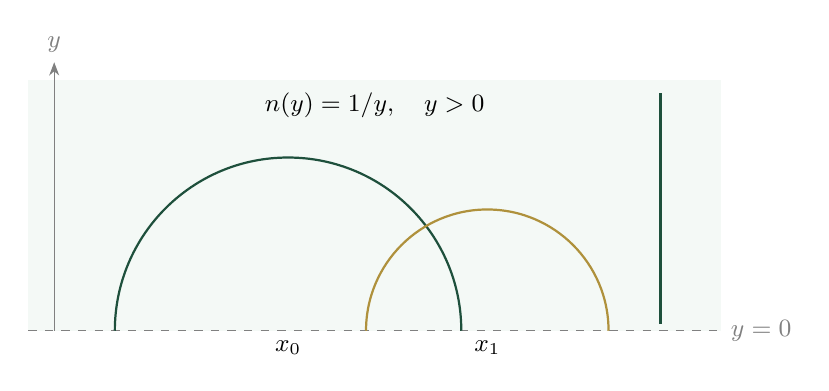
\begin{tikzpicture}[>=Stealth,font=\small,x=1.1cm,y=1.1cm]
 \fill[GreenPale,opacity=.3] (-4,0) rectangle(4,2.9);
 \draw[gray,dashed] (-4,0)--(4,0) node[right]{$y=0$};
 \draw[->,gray] (-3.7,0)--(-3.7,3.1) node[above]{$y$};
 \draw[GreenMain,thick] (1,0) arc[start angle=0,end angle=180,radius=2];
 \draw[GoldMain,thick] (2.7,0) arc[start angle=0,end angle=180,radius=1.4];
 \draw[GreenMain,thick] (3.3,.08)--(3.3,2.75);
 \node at (0,2.6){$n(y)=1/y,\quad y>0$};
 \node[below] at (-1,0){$x_0$};\node[below] at (1.3,0){$x_1$};
\end{tikzpicture}
\captionof{figure}{折射率 $n(y)=1/y$ 时的射线：与边界正交的半圆及竖直直线。}
\label{fig:ode-tikz-optical-geodesics}
\end{minipage}
\end{center}

\section{一维二重零点的光滑正规形}

\begin{definition}
方程在允许的局部坐标变换下化成的简化表达式称为正规形。
在所有这类变换下不变的参数称为模参数。
\end{definition}
\begin{theorem}
设 $v\in C^\infty$，$v(x)=ax^2+bx^3+O(x^4)$，$a\ne0$。
存在零点附近的光滑坐标 $y=g(x)$，使 $x'=v(x)$ 化为
\[
 y'=y^2+Cy^3,\qquad C=b/a^2.
\]
$C$ 在保持时间参数不变的光滑坐标变换下不变。
\end{theorem}
\begin{proof}
由 Taylor 除法，零点两侧的积分时间函数可统一写成
\[
 V(x)=-\frac1{ax}-C\log|x|+R(x),
\]
其中 $R$ 光滑；因为 $1/v=1/(ax^2)-C/x+$ 一个光滑函数。
目标场的积分时间同样为
$W(y)=-1/y-C\log|y|+S(y)$，$S$ 光滑。
寻找 $y=ax(1+xh(x))$ 并使 $W(y)=V(x)$。
消去两侧相同的奇性后，方程成为
\[
 \frac{h}{a(1+xh)}-C\log|a|-C\log(1+xh)
 +S(ax(1+xh))-R(x)=0.
\]
这是 $(x,h)$ 的光滑方程，在 $x=0$ 对 $h$ 的导数为 $1/a\ne0$。
先由零阶方程选唯一 $h(0)$，再由隐函数定理得到光滑 $h(x)$。
于是 $g'(0)=a\ne0$，是局部微分同胚。
对时间函数恒等式求导，
\[
 g'(x)/[g(x)^2+Cg(x)^3]=1/v(x),
\]
所以 $g'(x)v(x)=g(x)^2+Cg(x)^3$，完成正规化。

若任意换元 $y=sx+tx^2+O(x^3)$，计算新右端二、三次系数分别为
$\widetilde a=a/s$、$\widetilde b=b/s^2$。
因此 $\widetilde b/\widetilde a^2=b/a^2$，证明不变量结论。
\end{proof}

\section{广义 Lotka--Volterra 系统没有孤立闭轨}
考虑
\[
 P=x(a+kx+ly),\qquad Q=y(b+mx+ny).
\]
\begin{theorem}
上述系统没有极限环。若存在非平衡闭轨，则它附近充满闭轨。
\end{theorem}
\begin{proof}
坐标轴是不变集，因此闭轨不能穿过它们。各象限作符号换元可归为正象限。
先设 $kn-lm\ne0$。取 $\alpha,\beta$ 解
\[
 k\alpha+m\beta=-k,\qquad l\alpha+n\beta=-n.
\]
令 $B=x^{\alpha-1}y^{\beta-1}>0$，计算得
\[
 \partial_x(BP)+\partial_y(BQ)
 =B(\alpha a+\beta b).
\]
若常数 $\alpha a+\beta b\ne0$，前文的 Dulac 判据在单连通正象限排除所有闭轨。
若该常数为零，1-形式 $-BQ\,dx+BP\,dy$ 闭，
在凸的正象限有势函数 $H$，满足 $H_x=-BQ,H_y=BP$。
沿轨道 $\dot H=0$，且在非平衡闭轨附近 $\nabla H\ne0$。
闭轨的紧性和隐函数定理把附近等值集写成一族邻近光滑闭曲线；
场沿每条曲线相切且非零，所以每条都是闭轨，原闭轨不孤立。

若 $kn-lm=0$，正象限内平衡方程为两条线性方程。
它们要么无公共解，要么公共解包含一条直线（含全平面的更退化情形）。
任何闭轨围成的盘内必有平衡点，因为其边界场沿切线转一圈，指标为 1。
若平衡点集含直线，则从盘内该点沿直线继续，必穿过闭轨边界，
但边界不含平衡点，矛盾。无平衡点的情形也与边界指标矛盾。
所以退化行列式情形没有闭轨。
\end{proof}

\section{圆周上的小扩散与稳态集中}
令圆周长度为 $L$，$b(x+L)=b(x)$，$\varepsilon>0$。
密度方程为
\[
 u_t=\varepsilon u_{xx}-(b(x)u)_x,\qquad
 \int_0^L u\,dx=1.
\]

\begin{definition}[周期密度与经典解]
圆周上的概率密度指非负的 $L$ 周期连续函数 $u$，满足 $\displaystyle\int_0^Lu(x)dx=1$；
对一段圆弧赋予的质量为其上 $u$ 的积分。
含时间的经典解在这里指具有连续 $u_t,u_x,u_{xx}$ 并逐点满足密度方程的周期函数。
$L^1$ 距离在本章指 $\|u-v\|_1=\displaystyle\int_0^L|u-v|dx$，所有函数光滑，均为通常积分。
概率流 $J$ 以守恒式 $u_t=-J_x$ 定义其输运意义，不预设随机过程的一般理论。
\end{definition}

\begin{definition}
概率流为 $J=bu-\varepsilon u_x$，方程即 $u_t=-J_x$。
在覆盖直线上选势 $U'=-b$，有 $U(x+L)=U(x)+c$。
不显含时间的归一化正密度称稳态。
\end{definition}
\begin{proposition}
若 $c=0$，稳态为 Gibbs 型密度
\[
 \rho=C_\varepsilon e^{-U/\varepsilon}.
\]
一般情形可统一写成
\[
 \rho(x)=C_\varepsilon e^{-U(x)/\varepsilon}
 \int_x^{x+L}e^{U(s)/\varepsilon}\,ds,
\]
常数使积分为 1；它光滑、严格为正并且周期。
\end{proposition}
\begin{proof}
稳态方程为 $(b\rho-\varepsilon\rho')'=0$，故概率流为常数 $J$，即
$\varepsilon\rho'+U'\rho=-J$。积分因子给出
\[
 (e^{U/\varepsilon}\rho)'=-\frac{J}{\varepsilon}e^{U/\varepsilon}.
\]
令 $I(x)=\displaystyle\int_x^{x+L}e^{U(s)/\varepsilon}\,ds>0$。因 $U(x+L)=U(x)+c$，有
\[
 I'(x)=e^{U(x+L)/\varepsilon}-e^{U(x)/\varepsilon}
 =(e^{c/\varepsilon}-1)e^{U(x)/\varepsilon}.
\]
所以 $\rho=C_\varepsilon e^{-U/\varepsilon}I$ 满足
\[
 \varepsilon\rho'+U'\rho=\varepsilon C_\varepsilon(e^{c/\varepsilon}-1),
\]
确为常流稳态。
又 $I(x+L)=e^{c/\varepsilon}I(x)$，与前面的指数因子抵消，故 $\rho$ 周期。
其严格正性保证可选唯一正数 $C_\varepsilon$ 使总积分为 1。

证明唯一性时，先设 $c\ne0$。将积分因子等式在 $[x,x+L]$ 上积分，
对任意周期稳态均得
\[
 (e^{c/\varepsilon}-1)e^{U(x)/\varepsilon}\rho(x)
 =-\frac{J}{\varepsilon}I(x).
\]
故所有周期稳态都为上述正函数的常数倍，再由归一化唯一确定。
若 $c=0$，同一等式给出 $JI(x)=0$，所以 $J=0$。
积分因子方程随即给出 $\rho=C e^{-U/\varepsilon}$，归一化后也唯一。
此时 $e^{U/\varepsilon}$ 为周期函数，故积分 $I(x)$ 与 $x$ 无关，
故一般公式正好化为 Gibbs 型表达式。
\end{proof}
\begin{theorem}[稳态的吸引性]
对存在的光滑周期解，密度趋于上述唯一稳态；更准确地，
$\displaystyle\int\rho(u/\rho-1)^2$ 指数衰减。
\end{theorem}
\begin{proof}
固定 $\varepsilon>0$，令 $w=u/\rho$。将 $u=\rho w$ 代入密度方程，
利用 $(\varepsilon\rho'-b\rho)'=0$ 和 $J=b\rho-\varepsilon\rho'$，整理得
\[
 \rho w_t=\varepsilon(\rho w_x)_x-Jw_x.
\]
记 
\[
 \mathcal E(t)=\displaystyle\int_0^L\rho(w-1)^2\,dx.
\]
由于 $\rho$ 不依赖时间，
乘 $w-1$ 并积分，周期边界项消失，有
\begin{align*}
 \tfrac12\mathcal E'(t)
 &=-\varepsilon\int_0^L\rho w_x^2\,dx
   -J\int_0^L(w-1)w_x\,dx\\
 &=-\varepsilon\int_0^L\rho w_x^2\,dx.
\end{align*}
最后一个积分为 $\tfrac12[(w-1)^2]_0^L=0$；因此即使稳态流不为零，耗散恒等式仍成立。

归一化给出 $\displaystyle\int_0^L\rho(w-1)\,dx=0$。因 $\rho>0$ 且 $w$ 连续，
若 $w$ 不恒等于 1，必在某点 $x_0$ 取值 1。
沿圆周长度不超过 $L$ 的一条弧，从该点积分并用 Cauchy--Schwarz，得到
\[
 |w(x)-1|^2\leq L\int_0^L|w_x|^2\,dx
 \leq\frac{L}{m}\int_0^L\rho w_x^2\,dx,
 \qquad m=\min_{[0,L]}\rho>0.
\]
再乘 $\rho$ 积分，并用 $\displaystyle\int\rho=1$，得
\[
 \mathcal E\leq(L/m)\displaystyle\int\rho w_x^2.
\]
当 $w\equiv1$ 时此式也成立。
因此 $\mathcal E'\leq-(2\varepsilon m/L)\mathcal E$，积分得到
\[
 \mathcal E(t)\leq\mathcal E(0)e^{-2\varepsilon mt/L}.
\]
这就是所述加权平方平均意义下的指数吸引性。
它还蕴含 $L^1$ 收敛，因为
\[
 \begin{aligned}
 \int_0^L|u-\rho|\,dx
 &\leq\left(\int\rho\right)^{1/2}\mathcal E^{1/2}\\
 &=\mathcal E^{1/2}.
\end{aligned}
\]
上述证明以光滑周期解的存在性为假设，不涉及该偏微分方程解的存在性。
\end{proof}

\begin{definition}[密度的集中与弱收敛]\label{def:density-concentration}
概率密度 $\rho_\varepsilon$ 集中于闭集 $K$，是指对每个包含 $K$ 的开邻域 $V$，
$\displaystyle\int_{V^c}\rho_\varepsilon dx\to0$。
称它弱收敛到 $x_*$ 处的单位质量，是指对每个连续周期函数 $f$ 都有
\[
 \int_0^Lf(x)\rho_\varepsilon(x)dx\longrightarrow f(x_*).
\]
这不是逐点收敛。若密度集中于唯一点 $x_*$，在该点的小邻域内用 $f$ 的一致连续性控制差，
邻域外用 $2\|f\|_\infty$ 乘以趋零的质量控制差，即得到上述弱收敛。

\end{definition}

\begin{proposition}[小扩散极限]
若周期势 $U$ 有唯一全局最小点，则 $\rho$ 在 $\varepsilon\downarrow0$ 时集中于该点。
一般情形定义
$D(x)=\max_{x\leq s\leq x+L}U(s)-U(x)$，
则稳态质量集中在 $D$ 的最大点集合；若该最大点唯一，则收敛为该点的单位质量。
\end{proposition}
\begin{proof}
紧圆上的 Laplace 估计给出
$\varepsilon\log\displaystyle\int_x^{x+L}e^{U(s)/\varepsilon}ds
\to\max_{[x,x+L]}U$，并且关于 $x$ 一致。
上界由区间长度乘最大指数得到；下界用 $U$ 的统一 Lipschitz 常数，
在最大点附近长度为 $O(\varepsilon)$ 的区间上，$U$ 至少为最大值减 $O(\varepsilon)$，
所以对数下界与上界差趋于零。
因此，在未确定归一化常数时，密度的对数乘以扩散系数后趋于 $D(x)$。
最大点集合之外的任一闭集都与最大值有严格正间隙，
该闭集上的质量与最大点邻域内质量之比按指数趋于零，故归一化后该闭集上的质量趋于零。
对于周期势，每个周期区间内的最大值均为 $\max U$，所以 $D$ 的最大点恰是 $U$ 的最小点。
\end{proof}
势能有多个取到相同最小值的点时，前述结论只保证密度集中于这些点所成的集合。各点附近质量的比例还须根据相应积分的渐近值确定。

图~\ref{fig:ode-tikz-gibbs-concentration} 取周期势 $U=1-\cos x$，两条密度曲线均已归一化。
\begin{center}
\begin{minipage}{0.96\linewidth}
\centering
% TikZ mathematical illustration; compiled with the main document.
\begin{tikzpicture}[>=Stealth,font=\small,x=1.3cm,y=1.6cm]

 \draw[->,gray] (-3.5,0)--(3.65,0) node[right]{$x$};
 \draw[->,gray] (0,0)--(0,1.35) node[above]{$\rho_\varepsilon$};
\draw[GoldMain,thick,domain=-3.14159:3.14159,samples=120] plot (\x,{exp(-(1-cos(\x r))/0.8)/2.575076472});
\draw[GreenMain,thick,domain=-3.14159:3.14159,samples=120] plot (\x,{exp(-(1-cos(\x r))/0.2)/1.153220937});

 \node[below] at (-3.14159,0){$-\pi$};\node[below] at (3.14159,0){$\pi$};
 \node[GreenMain,anchor=west] at (1.3,1.05){$\varepsilon=0.2$};
 \node[GoldMain,anchor=west] at (1.3,.7){$\varepsilon=0.8$};
 \node at (0,-.65){$U(x)=1-\cos x$，两端按圆周粘合};
\end{tikzpicture}
\captionof{figure}{同一周期势的归一化 Gibbs 稳态；扩散变小时，质量更集中于唯一势阱 $x=0$。}
\label{fig:ode-tikz-gibbs-concentration}
\end{minipage}
\end{center}

\setchapterimage{figure/Chapter15封面图.jpg}
\setchapterintro{用压缩映射构造稳定流形，用反对称函数讨论 Sturm 特征函数线性组合的零点，再说明隐式方程与快慢系统的折叠奇点。超出常微分方程基础的分析与分类前提会单独列明。}
\chapter{不变流形与进阶专题}\label{chap:invariant-manifolds}

第六章的线性近似给出稳定性判据，第~\ref{chap:linear-conjugacy}~章则分类双曲线性系统。下面用压缩映射构造非线性不变流形及局部共轭；后两节分别回到第~\ref{chap:sturm}~章的零点问题和第~\ref{chap:characteristics}~章的隐式方程几何。

\section{双曲映射的稳定与不稳定流形}
下面将轨道的递推关系写成序列空间中的压缩方程，再由不动点构造局部不变流形。
\begin{definition}
设局部微分同胚 $F(0)=0$。若 $DF(0)$ 无模为 1 的特征值，称零点双曲。
局部稳定集是正次迭代一直留在指定小邻域并趋于零的点集；
不稳定集对反向迭代作相同定义。
\end{definition}

\begin{definition}[映射的稳定子空间与局部不变性]
对可逆矩阵 $A$，其模小于 1 的广义特征空间的实直和记为 $E^s$，模大于 1 者记为 $E^u$。
这与连续流按特征值实部正负划分不同；时间 $\tau$ 映射的特征值为 $e^{\tau\lambda}$，才将两种划分联系起来。
子集局部不变，是指点及其像都留在规定邻域时，映射将集合内的点仍送到该集合内。
子流形在零点与 $E^s$ 相切，是指 $T_0W=E^s$。
\end{definition}
\begin{definition}[等价范数与加权序列空间]\label{def:weighted-banach}
两个范数等价，是指存在 $c,C>0$ 使 $c\|x\|_1\leq\|x\|_2\leq C\|x\|_1$。
固定 $0<\sigma\leq1$，记
\[
 X_\sigma=\{z=(z_n)_{n\geq0}:\|z\|_\sigma:=\sup_{n\geq0}\sigma^{-n}|z_n|<\infty\}.
\]
这是 Banach 空间：加权 Cauchy 列在每个坐标有极限，统一的 Cauchy 界对坐标取极限后仍成立，
因而所得极限仍在 $X_\sigma$，且依此范数收敛。
特别地 $X_1=\ell^\infty$ 是有界序列空间。
\end{definition}
\begin{definition}[Banach 空间中的微分]\label{def:frechet-derivative}
对 Banach 空间间的映射 $F:U\subset X\to Y$，若存在有界线性映射 $A$ 使
\[
 \frac{\|F(x+h)-F(x)-Ah\|_Y}{\|h\|_X}\longrightarrow0,
\]
则称 $F$ 在 $x$ 处 Fréchet 可微，记 $DF(x)=A$。
若导数按算子范数连续，称 $F\in C^1$；将导数继续作为映射求导，定义 $C^r$。
高阶导数是连续多重线性映射，其范数是各个自变量的范数均不超过 1 时，函数值范数的上确界。
在有限维空间中，这就是全微分的线性主部定义。
后面的不动点导数公式会直接估计这一余项，不调用无穷维隐函数定理。
\end{definition}

\begin{theorem}[局部稳定流形]\label{thm:arnold-stable-manifold}
设 $F\in C^r$，$r\geq1$，零点双曲。
则在零点附近存在 $C^r$ 稳定与不稳定流形，分别与 $DF(0)$ 的稳定、不稳定子空间相切，
维数等于这些子空间维数；它们局部不变。
\end{theorem}
\begin{proof}
\paragraph{线性分解与截断。}
在稳定、不稳定子空间中分别取坐标，写成
\[
 \begin{aligned}
 F(u,v)&=(Su+f(u,v),Uv+g(u,v)),\\
 f(0)&=g(0)=0,\qquad Df(0)=Dg(0)=0.
\end{aligned}
\]
对 Jordan 块中的基向量作逐次缩放，可取等价范数，使
$\|S\|,\|U^{-1}\|\leq a<1$。两个子空间的乘积使用最大范数。
在半径 $r$ 的小球内，$Df,Dg$ 的范数随 $r\downarrow0$ 一致趋零。
取在半径 $r$ 球内为 1、半径 $2r$ 球外为零的光滑截断函数 $\chi_r$。
因 $|f(z)|,|g(z)|=o(|z|)$ 且 $|D\chi_r|=O(1/r)$，
乘积求导中的 $D\chi_r f,D\chi_r g$ 也一致趋零。
因此截断后的非线性项可具有任意小的全局 Lipschitz 常数 $L$。
以下先研究截断方程，最后限制回原小球。

\paragraph{将递推写成压缩方程。}
选 $a<\sigma<1$，在序列空间中置
\[
 \|z\|_\sigma=\sup_{n\geq0}\sigma^{-n}\max(|u_n|,|v_n|).
\]
乘以权 $\sigma^{-n}$ 将它等距对应到有界序列空间，因此该空间完备。
固定稳定坐标 $u_0=\xi$，定义算子 $\mathcal A_\xi$：
\begin{align*}
 (\mathcal A_\xi z)^s_n
 &=S^n\xi+\sum_{j=0}^{n-1}S^{n-1-j}f(z_j),\\
 (\mathcal A_\xi z)^u_n
 &=-\sum_{j=n}^\infty U^{n-1-j}g(z_j).
\end{align*}
第一式是稳定递推的逐次代入。第二式由
\[
 v_n=U^{-1}v_{n+1}-U^{-1}g(z_n)
\]
 向未来迭代，并令终点趋于无穷得到。
若 $z$ 有界，则剩余项 $U^{n-N}v_N$ 因 $\|U^{-1}\|<1$ 而趋零。
反过来，把第二个和式的 $n$ 与 $n+1$ 项相减，即得不稳定分量的原递推式，
故不动点确实给出一条轨道。

设 $d=\|z-\widetilde z\|_\sigma$。逐项估计为
\begin{align*}
 \sigma^{-n}|(\mathcal A_\xi z-\mathcal A_\xi\widetilde z)^s_n|
 &\leq Ld\sum_{j=0}^{n-1}a^{n-1-j}\sigma^{j-n}
 \leq\frac{L}{\sigma-a}d,\\
 \sigma^{-n}|(\mathcal A_\xi z-\mathcal A_\xi\widetilde z)^u_n|
 &\leq Ld\sum_{j=n}^\infty a^{j+1-n}\sigma^{j-n}
 =\frac{La}{1-a\sigma}d.
\end{align*}
将零序列代入算子，所得序列为 $(S^n\xi,0)$，其范数不超过 $|\xi|$。
所以算子将该空间映到自身。取 $L$ 使两常数的最大值 $q<1$，
Banach 定理给出唯一不动点 $z(\xi)$，且
\[
 \begin{aligned}
 \|z(\xi)\|_\sigma&\leq\frac{|\xi|}{1-q},\\
 \|z(\xi)-z(\eta)\|_\sigma&\leq\frac{|\xi-\eta|}{1-q}.
\end{aligned}
\]
因此这些轨道以 $\sigma^n$ 速度趋零。定义 $h(\xi)=v_0(\xi)$。
当 $|\xi|$ 足够小时，整条轨道均留在截断未改变方程的小球内。

\paragraph{光滑性与相切性。}
截断非线性项的各阶导数有界。将它逐项作用于加权序列，
其一阶余项由 $Df,Dg$ 的一致连续性控制。
第 $k$ 阶导数作用在 $k$ 个序列上时，每项的估计中含有因子 $\sigma^{kj}$；
因 $\sigma^{kj}\leq\sigma^j$，上述两种几何级数估计仍适用。
所以 $\mathcal A(\xi,z)$ 是 $C^r$ 映射，且 $\|D_z\mathcal A\|\leq q<1$。
从而
\[
 (I-D_z\mathcal A)^{-1}=\sum_{j=0}^\infty(D_z\mathcal A)^j,
 \qquad\|(I-D_z\mathcal A)^{-1}\|\leq(1-q)^{-1}.
\]
对不动点方程作差，并用刚得的 Lipschitz 估计控制其余项，得到
\[
 D_\xi z=(I-D_z\mathcal A)^{-1}D_\xi\mathcal A.
\]
由于余项除以 $|\Delta\xi|$ 后趋于零，上式即为 Fréchet 导数。
右端连续，因而 $z$ 为 $C^1$；继续求导时，最高阶未知导数仍乘
$I-D_z\mathcal A$，其余项只含已得到的低阶导数。由归纳得到 $C^r$。
取零初值，唯一不动点为零序列。由于 $Df(0)=Dg(0)=0$，
导数轨道恰为 $(S^n\xi,0)$，故 $h(0)=0,Dh(0)=0$。
图像 $\xi\mapsto(\xi,h(\xi))$ 的微分含恒等的第一分量，
是 $\dim E^s$ 维 $C^r$ 子流形，并与 $E^s$ 相切。

\paragraph{刻画局部稳定集。}
下面证明，始终留在所取邻域内的正向轨道，其初值均在上述图像上。在不加权有界序列空间中，
同一算子的压缩常数分别为 $L/(1-a)$ 和 $La/(1-a)$。
进一步缩小 $L$，使它们也小于 1。任何始终留在小球的正向轨道都是有界序列，
由前面的递推求和满足同一个不动点方程。
有界不动点唯一，而已构造的加权不动点也是有界的，故两者相同。
所以这类轨道自动趋零，其初点必在图像上。
反之，图像上足够靠近零的点，其估计保证整条正向轨道留在小球并趋零。
在选择的局部邻域内，这正是局部稳定集。
将轨道序列左移一项仍是趋零轨道，故其下一点也在图像上，得到局部不变性。
对局部逆映射 $F^{-1}$ 重复同一构造，得到不稳定流形。
\end{proof}
\begin{corollary}
自治 $C^r$ 向量场的双曲平衡点有相应局部稳定与不稳定流形。
\end{corollary}
\begin{proof}
取足够小的正时间 $\tau$，时间 $\tau$ 映射的导数为 $e^{\tau A}$。
其特征值模是 $e^{\tau\operatorname{Re}\lambda}$，所以双曲。
应用映射的稳定流形定理，再由相流在 $[0,\tau]$ 内的连续性，估计相邻两个整数倍时刻之间的解。
小时间的相流与上述时间映射可交换，故保持局部稳定集，因此所得图像对相流也局部不变。
\end{proof}


图~\ref{fig:ode-tikz-stable-manifolds} 的曲线由局部换元 $(u,v)=(s+0.18r^2,r+0.18s^2)$ 得到，故两条不变曲线在原点的切线分别是稳定与不稳定子空间。
\begin{center}
\begin{minipage}{0.96\linewidth}
\centering
% TikZ mathematical illustration; compiled with the main document.
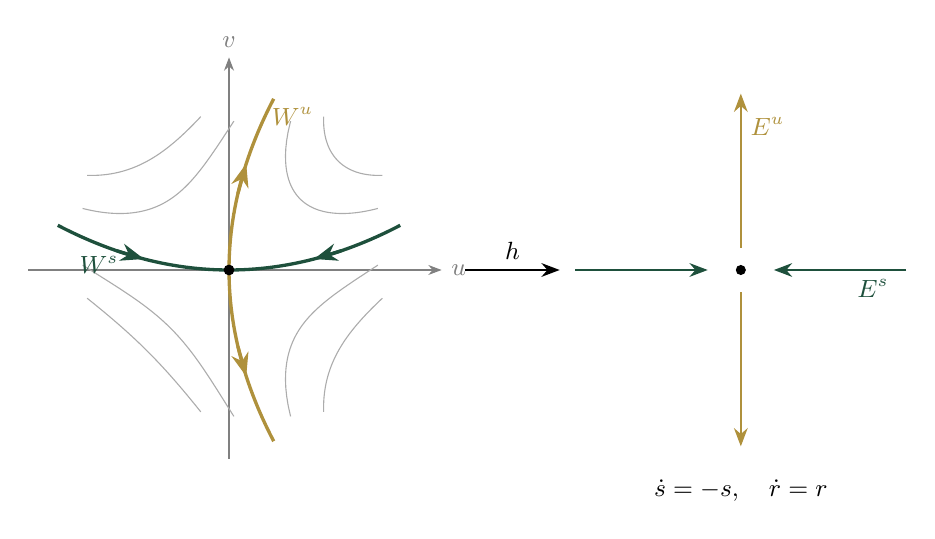
\begin{tikzpicture}[>=Stealth,font=\small]
\begin{scope}[scale=1.5]
 \draw[->,gray] (-1.7,0)--(1.8,0) node[right]{$u$};
 \draw[->,gray] (0,-1.6)--(0,1.8) node[above]{$v$};
\draw[gray!65,thin] plot coordinates {(-0.23875,1.29867) (-0.26634,1.26956) (-0.29290,1.24208) (-0.31853,1.21612) (-0.34331,1.19158) (-0.36733,1.16836) (-0.39064,1.14637) (-0.41332,1.12555) (-0.43541,1.10581) (-0.45696,1.08710) (-0.47802,1.06935) (-0.49863,1.05252) (-0.51882,1.03655) (-0.53863,1.02139) (-0.55808,1.00700) (-0.57720,0.99334) (-0.59602,0.98038) (-0.61455,0.96808) (-0.63282,0.95641) (-0.65084,0.94534) (-0.66863,0.93484) (-0.68621,0.92489) (-0.70359,0.91546) (-0.72078,0.90654) (-0.73780,0.89809) (-0.75465,0.89011) (-0.77135,0.88256) (-0.78790,0.87544) (-0.80432,0.86873) (-0.82061,0.86242) (-0.83678,0.85648) (-0.85284,0.85091) (-0.86878,0.84569) (-0.88463,0.84081) (-0.90038,0.83626) (-0.91605,0.83203) (-0.93162,0.82810) (-0.94711,0.82448) (-0.96253,0.82114) (-0.97788,0.81809) (-0.99315,0.81531) (-1.00836,0.81279) (-1.02351,0.81054) (-1.03859,0.80853) (-1.05362,0.80676) (-1.06860,0.80524) (-1.08352,0.80394) (-1.09840,0.80287) (-1.11323,0.80202) (-1.12801,0.80138) (-1.14275,0.80095) (-1.15745,0.80073) (-1.17212,0.80071) (-1.18674,0.80088) (-1.20133,0.80125)};
\draw[gray!65,thin] plot coordinates {(0.80125,-1.20133) (0.80070,-1.16709) (0.80117,-1.13435) (0.80258,-1.10300) (0.80484,-1.07294) (0.80786,-1.04406) (0.81158,-1.01629) (0.81594,-0.98955) (0.82089,-0.96377) (0.82637,-0.93887) (0.83235,-0.91482) (0.83878,-0.89154) (0.84562,-0.86899) (0.85285,-0.84713) (0.86044,-0.82590) (0.86835,-0.80527) (0.87658,-0.78521) (0.88508,-0.76568) (0.89385,-0.74665) (0.90287,-0.72808) (0.91211,-0.70996) (0.92157,-0.69225) (0.93123,-0.67493) (0.94107,-0.65798) (0.95109,-0.64138) (0.96128,-0.62511) (0.97162,-0.60915) (0.98210,-0.59348) (0.99272,-0.57809) (1.00346,-0.56296) (1.01433,-0.54808) (1.02531,-0.53344) (1.03640,-0.51901) (1.04759,-0.50479) (1.05888,-0.49077) (1.07025,-0.47694) (1.08171,-0.46329) (1.09326,-0.44980) (1.10488,-0.43647) (1.11657,-0.42329) (1.12833,-0.41025) (1.14016,-0.39734) (1.15205,-0.38456) (1.16400,-0.37190) (1.17601,-0.35935) (1.18807,-0.34691) (1.20018,-0.33456) (1.21234,-0.32231) (1.22455,-0.31015) (1.23680,-0.29807) (1.24910,-0.28607) (1.26144,-0.27414) (1.27381,-0.26228) (1.28622,-0.25049) (1.29867,-0.23875)};
\draw[gray!65,thin] plot coordinates {(0.04125,1.26037) (-0.01665,1.17167) (-0.06689,1.09529) (-0.11135,1.02892) (-0.15136,0.97078) (-0.18788,0.91952) (-0.22164,0.87407) (-0.25318,0.83355) (-0.28292,0.79729) (-0.31117,0.76471) (-0.33820,0.73534) (-0.36420,0.70880) (-0.38934,0.68476) (-0.41375,0.66295) (-0.43753,0.64312) (-0.46077,0.62508) (-0.48355,0.60866) (-0.50593,0.59371) (-0.52795,0.58009) (-0.54967,0.56769) (-0.57111,0.55642) (-0.59232,0.54617) (-0.61331,0.53689) (-0.63412,0.52848) (-0.65475,0.52091) (-0.67524,0.51410) (-0.69559,0.50801) (-0.71581,0.50259) (-0.73593,0.49781) (-0.75594,0.49362) (-0.77587,0.49000) (-0.79571,0.48691) (-0.81548,0.48433) (-0.83518,0.48224) (-0.85481,0.48060) (-0.87439,0.47940) (-0.89391,0.47862) (-0.91339,0.47824) (-0.93282,0.47825) (-0.95221,0.47862) (-0.97156,0.47936) (-0.99087,0.48043) (-1.01015,0.48184) (-1.02940,0.48357) (-1.04863,0.48561) (-1.06782,0.48795) (-1.08699,0.49058) (-1.10614,0.49350) (-1.12526,0.49669) (-1.14437,0.50015) (-1.16346,0.50387) (-1.18252,0.50785) (-1.20158,0.51207) (-1.22061,0.51654) (-1.23963,0.52125)};
\draw[gray!65,thin] plot coordinates {(0.52125,-1.23963) (0.50076,-1.14758) (0.48792,-1.06759) (0.48087,-0.99735) (0.47827,-0.93510) (0.47916,-0.87948) (0.48280,-0.82940) (0.48867,-0.78402) (0.49634,-0.74264) (0.50549,-0.70468) (0.51587,-0.66969) (0.52728,-0.63727) (0.53955,-0.60711) (0.55255,-0.57891) (0.56617,-0.55245) (0.58034,-0.52753) (0.59497,-0.50397) (0.61000,-0.48163) (0.62538,-0.46037) (0.64107,-0.44008) (0.65703,-0.42066) (0.67324,-0.40203) (0.68965,-0.38409) (0.70625,-0.36679) (0.72303,-0.35006) (0.73995,-0.33385) (0.75701,-0.31810) (0.77419,-0.30278) (0.79148,-0.28784) (0.80887,-0.27324) (0.82635,-0.25896) (0.84392,-0.24496) (0.86156,-0.23121) (0.87927,-0.21770) (0.89704,-0.20439) (0.91487,-0.19127) (0.93275,-0.17832) (0.95069,-0.16551) (0.96866,-0.15284) (0.98668,-0.14029) (1.00474,-0.12784) (1.02283,-0.11548) (1.04096,-0.10321) (1.05912,-0.09100) (1.07730,-0.07885) (1.09551,-0.06675) (1.11375,-0.05469) (1.13201,-0.04266) (1.15029,-0.03065) (1.16859,-0.01867) (1.18692,-0.00669) (1.20525,0.00529) (1.22361,0.01726) (1.24198,0.02925) (1.26037,0.04125)};
\draw[gray!65,thin] plot coordinates {(0.04125,-1.23963) (-0.01665,-1.14758) (-0.06689,-1.06759) (-0.11135,-0.99735) (-0.15136,-0.93510) (-0.18788,-0.87948) (-0.22164,-0.82940) (-0.25318,-0.78402) (-0.28292,-0.74264) (-0.31117,-0.70468) (-0.33820,-0.66969) (-0.36420,-0.63727) (-0.38934,-0.60711) (-0.41375,-0.57891) (-0.43753,-0.55245) (-0.46077,-0.52753) (-0.48355,-0.50397) (-0.50593,-0.48163) (-0.52795,-0.46037) (-0.54967,-0.44008) (-0.57111,-0.42066) (-0.59232,-0.40203) (-0.61331,-0.38409) (-0.63412,-0.36679) (-0.65475,-0.35006) (-0.67524,-0.33385) (-0.69559,-0.31810) (-0.71581,-0.30278) (-0.73593,-0.28784) (-0.75594,-0.27324) (-0.77587,-0.25896) (-0.79571,-0.24496) (-0.81548,-0.23121) (-0.83518,-0.21770) (-0.85481,-0.20439) (-0.87439,-0.19127) (-0.89391,-0.17832) (-0.91339,-0.16551) (-0.93282,-0.15284) (-0.95221,-0.14029) (-0.97156,-0.12784) (-0.99087,-0.11548) (-1.01015,-0.10321) (-1.02940,-0.09100) (-1.04863,-0.07885) (-1.06782,-0.06675) (-1.08699,-0.05469) (-1.10614,-0.04266) (-1.12526,-0.03065) (-1.14437,-0.01867) (-1.16346,-0.00669) (-1.18252,0.00529) (-1.20158,0.01726) (-1.22061,0.02925) (-1.23963,0.04125)};
\draw[gray!65,thin] plot coordinates {(0.52125,1.26037) (0.50076,1.17167) (0.48792,1.09529) (0.48087,1.02892) (0.47827,0.97078) (0.47916,0.91952) (0.48280,0.87407) (0.48867,0.83355) (0.49634,0.79729) (0.50549,0.76471) (0.51587,0.73534) (0.52728,0.70880) (0.53955,0.68476) (0.55255,0.66295) (0.56617,0.64312) (0.58034,0.62508) (0.59497,0.60866) (0.61000,0.59371) (0.62538,0.58009) (0.64107,0.56769) (0.65703,0.55642) (0.67324,0.54617) (0.68965,0.53689) (0.70625,0.52848) (0.72303,0.52091) (0.73995,0.51410) (0.75701,0.50801) (0.77419,0.50259) (0.79148,0.49781) (0.80887,0.49362) (0.82635,0.49000) (0.84392,0.48691) (0.86156,0.48433) (0.87927,0.48224) (0.89704,0.48060) (0.91487,0.47940) (0.93275,0.47862) (0.95069,0.47824) (0.96866,0.47825) (0.98668,0.47862) (1.00474,0.47936) (1.02283,0.48043) (1.04096,0.48184) (1.05912,0.48357) (1.07730,0.48561) (1.09551,0.48795) (1.11375,0.49058) (1.13201,0.49350) (1.15029,0.49669) (1.16859,0.50015) (1.18692,0.50387) (1.20525,0.50785) (1.22361,0.51207) (1.24198,0.51654) (1.26037,0.52125)};
\draw[gray!65,thin] plot coordinates {(-0.23875,-1.20133) (-0.26634,-1.16709) (-0.29290,-1.13435) (-0.31853,-1.10300) (-0.34331,-1.07294) (-0.36733,-1.04406) (-0.39064,-1.01629) (-0.41332,-0.98955) (-0.43541,-0.96377) (-0.45696,-0.93887) (-0.47802,-0.91482) (-0.49863,-0.89154) (-0.51882,-0.86899) (-0.53863,-0.84713) (-0.55808,-0.82590) (-0.57720,-0.80527) (-0.59602,-0.78521) (-0.61455,-0.76568) (-0.63282,-0.74665) (-0.65084,-0.72808) (-0.66863,-0.70996) (-0.68621,-0.69225) (-0.70359,-0.67493) (-0.72078,-0.65798) (-0.73780,-0.64138) (-0.75465,-0.62511) (-0.77135,-0.60915) (-0.78790,-0.59348) (-0.80432,-0.57809) (-0.82061,-0.56296) (-0.83678,-0.54808) (-0.85284,-0.53344) (-0.86878,-0.51901) (-0.88463,-0.50479) (-0.90038,-0.49077) (-0.91605,-0.47694) (-0.93162,-0.46329) (-0.94711,-0.44980) (-0.96253,-0.43647) (-0.97788,-0.42329) (-0.99315,-0.41025) (-1.00836,-0.39734) (-1.02351,-0.38456) (-1.03859,-0.37190) (-1.05362,-0.35935) (-1.06860,-0.34691) (-1.08352,-0.33456) (-1.09840,-0.32231) (-1.11323,-0.31015) (-1.12801,-0.29807) (-1.14275,-0.28607) (-1.15745,-0.27414) (-1.17212,-0.26228) (-1.18674,-0.25049) (-1.20133,-0.23875)};
\draw[gray!65,thin] plot coordinates {(0.80125,1.29867) (0.80070,1.26956) (0.80117,1.24208) (0.80258,1.21612) (0.80484,1.19158) (0.80786,1.16836) (0.81158,1.14637) (0.81594,1.12555) (0.82089,1.10581) (0.82637,1.08710) (0.83235,1.06935) (0.83878,1.05252) (0.84562,1.03655) (0.85285,1.02139) (0.86044,1.00700) (0.86835,0.99334) (0.87658,0.98038) (0.88508,0.96808) (0.89385,0.95641) (0.90287,0.94534) (0.91211,0.93484) (0.92157,0.92489) (0.93123,0.91546) (0.94107,0.90654) (0.95109,0.89809) (0.96128,0.89011) (0.97162,0.88256) (0.98210,0.87544) (0.99272,0.86873) (1.00346,0.86242) (1.01433,0.85648) (1.02531,0.85091) (1.03640,0.84569) (1.04759,0.84081) (1.05888,0.83626) (1.07025,0.83203) (1.08171,0.82810) (1.09326,0.82448) (1.10488,0.82114) (1.11657,0.81809) (1.12833,0.81531) (1.14016,0.81279) (1.15205,0.81054) (1.16400,0.80853) (1.17601,0.80676) (1.18807,0.80524) (1.20018,0.80394) (1.21234,0.80287) (1.22455,0.80202) (1.23680,0.80138) (1.24910,0.80095) (1.26144,0.80073) (1.27381,0.80071) (1.28622,0.80088) (1.29867,0.80125)};

 \draw[GreenMain,very thick,domain=-1.45:1.45,samples=60] plot (\x,{.18*\x*\x});
 \draw[GoldMain,very thick,domain=-1.45:1.45,samples=60] plot ({.18*\x*\x},\x);
 \foreach \s/\t in {-.95/-.72,.95/.72}{\draw[GreenMain,->,very thick] (\s,{.18*\s*\s})--(\t,{.18*\t*\t});}
 \foreach \s/\t in {-.65/-.9,.65/.9}{\draw[GoldMain,->,very thick] ({.18*\s*\s},\s)--({.18*\t*\t},\t);}
 \node[GreenMain,below] at (-1.1,.2){$W^s$};\node[GoldMain,right] at (.28,1.3){$W^u$};
 \fill (0,0) circle(1.3pt);
\end{scope}
\draw[->,thick] (3,0)--(4.2,0) node[midway,above]{$h$};
\begin{scope}[shift={(6.5,0)},scale=1.4]
 \draw[->,GreenMain,thick] (-1.5,0)--(-.3,0);\draw[->,GreenMain,thick] (1.5,0)--(.3,0);
 \draw[->,GoldMain,thick] (0,.2)--(0,1.6);\draw[->,GoldMain,thick] (0,-.2)--(0,-1.6);
 \node[GreenMain,below] at (1.2,0){$E^s$};\node[GoldMain,right] at (0,1.3){$E^u$};
 \fill (0,0) circle(1.3pt);
 \node at (0,-2){$\dot s=-s,\quad\dot r=r$};
\end{scope}
\end{tikzpicture}
\captionof{figure}{局部稳定、不稳定流形及其线性模型；粗线箭头分别趋向和离开平衡点。}
\label{fig:ode-tikz-stable-manifolds}
\end{minipage}
\end{center}

\section{非线性双曲平衡点的局部共轭}
线性分类描述了双曲线性系统的相流。本节通过构造互逆的连续变换，将这一描述推广到非线性平衡点附近。
\begin{theorem}[局部双曲共轭]
设 $x'=Ax+R(x)$，$R(0)=0,DR(0)=0$，$A$ 双曲，$R\in C^1$。
原方程在零点附近与 $y'=Ay$ 局部拓扑共轭，并保持时间参数。
\end{theorem}
\begin{proof}
\paragraph{双曲线性方程的有界逆。}
记稳定、不稳定投影为 $P_s,P_u$。由广义特征空间分解和 Jordan 指数估计，
存在 $K,c>0$，使
\[
 \|e^{tA}P_s\|\leq Ke^{-ct}\ (t\geq0),\qquad
 \|e^{tA}P_u\|\leq Ke^{ct}\ (t\leq0).
\]

\noindent
这里 $P_s,P_u$ 是按直和 $\R^n=E^s\oplus E^u$ 分取两个分量的线性投影，
$P_s+P_u=I$。$C_b(\R,\R^n)$ 指全轴上有界连续函数，取范数
$\|f\|_\infty=\sup_{t\in\R}|f(t)|$。
一致 Cauchy 列一致收敛到有界连续函数，故它是 Banach 空间。
对非线性映射 $R$，$\operatorname{Lip}(R)$ 是所有满足
$|R(x)-R(y)|\leq L|x-y|$ 的常数 $L$ 的下确界。
\medskip

在有界连续函数的完备空间 $C_b(\R,\R^n)$ 中，定义
\[
 \begin{aligned}
 (Gf)(t)={}&\int_{-\infty}^te^{A(t-s)}P_sf(s)\,ds\\
 &-\int_t^\infty e^{A(t-s)}P_uf(s)\,ds.
\end{aligned}
\]
两积分绝对收敛，分别不超过 $K\|f\|_\infty/c$，故
$\|G\|\leq C_G:=2K/c$。在有限区间求导，再用指数尾项取极限，得
\[
 (Gf)'=A(Gf)+f.
\]
若两个有界特解存在，其差为 $e^{tA}v$；稳定分量若非零则负向无界，
不稳定分量若非零则正向无界。因而差为零，$Gf$ 是唯一整轴有界特解。
由积分换元还可知，$G$ 与任意时间平移可交换。

\paragraph{从非线性轨道得到线性轨道。}
用小球截断 $R$。因为 $R(0)=DR(0)=0$，截断后可同时做到
$\|R\|_\infty\leq M$、$\operatorname{Lip}(R)=L$，并使 $q=C_GL<1$。
该截断在一个零点邻域内不改变原方程。
截断方程的向量场满足线性增长估计
\[
 |Ax+R(x)|\leq\|A\||x|+M;
\]
Gronwall 估计及有限端点延拓判据
保证其解双向全局存在，记流为 $\varphi^t$。
对初点 $x_0$ 的整条轨道 $x(t)$，函数 $R(x(t))$ 有界。
置
\[
 y(t)=x(t)-G(R(x))(t).
\]
由 Green 算子的方程，
\[
 \begin{aligned}
 y'&=Ax+R(x)-[AG(R(x))+R(x)]\\
 &=A[x-G(R(x))]\\
 &=Ay.
\end{aligned}
\]
定义 $h(x_0)=y(0)$，时间平移可交换性于是给出
\[
 h(\varphi^tx_0)=e^{tA}h(x_0).
\]
此外 $|h(x_0)-x_0|\leq C_GM$。

\paragraph{构造逆变换并验证互逆。}
固定任意 $y_0$，令 $y(t)=e^{tA}y_0$。尽管 $y$ 本身可能无界，
映射 $z\mapsto G(R(y+z))$ 仍将 $C_b$ 映入自身，因为 $R$ 全局有界。
其 Lipschitz 常数不超过 $q<1$，故存在唯一有界不动点
\[
 z=G(R(y+z)),\qquad \|z\|_\infty\leq C_GM.
\]
于是 $z'=Az+R(y+z)$，所以 $x=y+z$ 解非线性方程。定义 $k(y_0)=x(0)$。
对于这条轨道，$G(R(x))=z$，故 $h(k(y_0))=y_0$。
反过来，对任意非线性轨道所定义的 $y=x-G(R(x))$，
有界差 $z=x-y$ 满足同一不动点方程。由唯一性，按逆变换求得的解就是该 $x$，
所以 $k(h(x_0))=x_0$。这证明 $h,k$ 是互逆双射，且 $h(0)=0$。

\paragraph{连续性。}
先证 $h$ 在任意 $x_0$ 连续。对 $G(R(\varphi^{\cdot}x_0))(0)$ 的积分，
$|s|>B$ 的尾项不超过 $2KM e^{-cB}/c$，且与初点无关。
先选大 $B$ 使尾项小，再用紧时间段 $[-B,B]$ 内的初值连续依赖，
使有限部分的积分连续，便得 $h$ 连续。

为证 $k$ 连续，从 $z_0=0$ 开始迭代
\[
 z_{j+1}=G(R(e^{\cdot A}y_0+z_j)).
\]
归纳地，每个 $z_j(t,y_0)$ 对 $(t,y_0)$ 连续：积分的远端仍由一致指数尾界控制，
有限部分使用被积函数在紧集上的连续性。
且压缩估计给出
\[
 \begin{aligned}
 \|z-z_j\|_\infty&\leq\frac{q^j}{1-q}\|z_1-z_0\|_\infty\\
 &\leq\frac{q^j C_GM}{1-q},
\end{aligned}
\]
这一界不依赖 $y_0$。因此 $z_j(0,y_0)$ 一致趋于连续函数 $z(0,y_0)$，
$k(y_0)=y_0+z(0,y_0)$ 连续。$h$ 因而是同胚。

最后取截断恒为 1 的零点邻域，并将全局共轭限制于该邻域及其像。
原方程的解若在一段时间内始终留在此邻域，就与截断方程的解相同，因而满足上述保持时间参数不变的共轭等式。
这正是原方程与线性方程的局部拓扑共轭。
\end{proof}

\section{特征函数线性组合的零点：反对称方法}

\begin{definition}[Dirichlet 算子、Rayleigh 商与算子性质]\label{def:dirichlet-rayleigh}
在有界区域 $\Omega\subset\R^d$ 上，记 $\Delta u=\sum_j\partial_{x_j}^2u$ 为 Laplace 算子。
给定连续实势 $V$，$Hu=-\Delta u+Vu$ 连同边界条件 $u|_{\partial\Omega}=0$，
称 Dirichlet Schrödinger 问题；方程 $Hu=\lambda u$ 的非零解称特征函数，$\lambda$ 称特征值。
对于零边界的分段光滑非零函数，其 Rayleigh 商定义为
\[
 \mathcal R[u]=\frac{\int_\Omega(|\nabla u|^2+V|u|^2)dx}
 {\int_\Omega|u|^2dx}.
\]
必要时先将光滑紧支撑函数按
$\|u\|_{H^1}^2=\displaystyle\int_\Omega(|u|^2+|\nabla u|^2)dx$ 完备化；所得空间记 $H_0^1(\Omega)$。
边界为零在这一完备化意义下解释。内积空间的完备化按定义~\ref{def:l2-completion} 的 Cauchy 列构造进行。
\end{definition}
\begin{definition}[紧算子、自伴与 Green 核]
Hilbert 空间上的有界线性算子 $T$ 自伴，是指 $\langle Tu,v\rangle=\langle u,Tv\rangle$。
$T$ 紧，是指任一有界序列的像都有范数收敛子列。
积分算子 $Tf(x)=\displaystyle\int K(x,y)f(y)dy$ 的函数 $K$ 称核；若 $T$ 是某个零边界微分问题的解算子，
则称 $K$ 为该问题的 Green 核。
最低特征值指全体特征值中的最小者，相应特征函数称最低特征函数；
“内部严格正”指 $u(x)>0$ 对每个 $x\in\Omega$ 成立。
最低特征函数的正性还须由下面的分析结论保证。
\end{definition}

以下使用两个分析预备定理：
\begin{enumerate}
 \item 一维正则 Dirichlet 边值算子的特征函数是 $L^2$ 的完全正交系。
 \item 有界连通区域的 Dirichlet Schrödinger 算子的最低特征函数可以取为内部严格正。
\end{enumerate}
前者由连续 Green 核的紧自伴谱定理得到；后者由 Rayleigh 商极小化、
取绝对值不增加能量及强最大值原理得到。
这里紧自伴谱定理的具体含义是：非零特征值为实数，每个非零特征空间有限维，
非零特征值若无限多只能趋于零；这些特征向量与核一起张成稠密子空间。
“最低”与“完全”分别按前面的 Rayleigh 商和平方平均稠密性解释。
这里明确列出这些前提，因为它们不是有限维矩阵谱定理或 ODE 的零点比较本身。

下面把正性论证中所用的强最大值原理的具体情形单独证明。
\begin{lemma}[非负经典解的强正性]\label{lem:nonnegative-elliptic-positive}
设 $\Omega\subset\R^d$ 连通，$c$ 连续，$u\in C^2(\Omega)$、$u\geq0$，且 $\Delta u=c(x)u$。
则 $u$ 恒为零或处处严格为正。特别地，非负非零经典特征函数在内部严格为正。
\end{lemma}
\begin{proof}
设 $u(x_0)=0$。在以 $x_0$ 为心、闭包包含于 $\Omega$ 的小球内取 $C\geq\sup|c|$，
令 $m(r)$ 为半径 $r$ 球面上 $u$ 的平均值，$m(0)=0$。
由极坐标积分和 Stokes 公式对 $\nabla u$ 的应用，
\[
 m'(r)=r^{1-d}\int_0^r s^{d-1}\operatorname{avg}_{|x-x_0|=s}\Delta u\,ds
 \leq C r^{1-d}\int_0^r s^{d-1}m(s)\,ds.
\]
这里球面平均是按单位球面的面积归一化的积分；在 $d=1$ 时就是两端点值的平均。
设 $M(r)=\max_{0\leq s\leq r}m(s)\geq0$。对上式从 0 积分到任意 $t\leq r$，得到
\[
 m(t)\leq \frac{Ct^2}{2d}M(r),\qquad
 M(r)\leq\frac{Cr^2}{2d}M(r).
\]
取 $r$ 使 $Cr^2/(2d)<1$，只能有 $M(r)=0$。
因 $u$ 非负且连续，每个球面平均为零迫使球面上处处为零，所以 $u$ 在整球内为零。
因此零点集既开又闭；连通性使它为空或整个 $\Omega$。
特征方程可写成 $\Delta u=(V-\lambda)u$，故得到最后的断言。
\end{proof}

\begin{definition}
交换任意两个变量都改变符号的函数称为反对称函数。
由 $n$ 个单变量函数构成的 Slater 行列式是
\[
 \Psi(x_1,\ldots,x_n)=\det(\phi_i(x_j))_{i,j=1}^n.
\]
有序单纯形为 
\[
 \Delta=\{0<x_1<\cdots<x_n<l\}.
\]
\end{definition}
\begin{theorem}
设 $\phi_1,\ldots,\phi_n$ 为一维正则 Dirichlet 问题的前 $n$ 个实特征函数，
按严格递增特征值排列。则它们的任意非零线性组合在 $(0,l)$ 至多有 $n-1$ 个不同零点。
\end{theorem}
\begin{proof}
令一维算子为 $H=-D^2-q$，特征值为 $\lambda_i$。
在立方体 $(0,l)^n$ 上，定义
\[
 H^{(n)}=\sum_{j=1}^n\bigl(-\partial_{x_j}^2-q(x_j)\bigr).
\]
对乘积基的特征值为各 $\lambda$ 的和。
在反对称子空间中，重复指标的乘积反对称化为零；
最小可能的和因此为 $\lambda_1+\cdots+\lambda_n$，其特征空间由 $\Psi$ 一维张成。

反对称函数在 $x_i=x_j$ 上为零，且 Dirichlet 条件使它在外边界也为零。
从 $\Delta$ 上的零边界函数按变量排列作带符号延拓，得到立方体的反对称函数；
两边 Rayleigh 商相同，因为各排列单纯形的能量与范数都相等。
因此 $\Psi|_\Delta$ 是单纯形上的最低特征函数。
由前述最低特征函数的严格正性及一维性，它在 $\Delta$ 内没有零点。

若非零组合 $f=\sum_{i=1}^nc_i\phi_i$ 在 $n$ 个不同内部点
$x_1<\cdots<x_n$ 为零，则向量 $(c_i)$ 是矩阵 $(\phi_i(x_j))$ 的非零左核向量。
于是 $\Psi(x_1,\ldots,x_n)=0$，与单纯形内部无零点矛盾。
所以至多有 $n-1$ 个不同零点。
\end{proof}
反对称化把线性组合的零点问题转成有序单纯形上的正性问题。

\section{折叠、对合与快慢系统}
下面研究隐式方程的曲面投影，以及投影奇点与慢运动之间的关系。
\begin{definition}
微分同胚 $\iota$ 若满足 $\iota^2=\operatorname{id}$，称为对合。
曲面投影若在某点局部等价于 $(s,r)\mapsto(s,r^2)$，称为折叠。
交换两个同投影点的局部对合 $(s,r)\mapsto(s,-r)$ 称其分支交换对合。
\end{definition}
\begin{proposition}
对隐式方程曲面 $E=\{F(t,x,p)=0\}$，若
\[
 F_p=0,\qquad F_{pp}\ne0,\qquad F_t+pF_x\ne0,
\]
则投影 $E\to(t,x)$ 在该点为折叠，接触迹方向场在那里非零并横截折叠点曲线。
\end{proposition}
\begin{proof}
$F_t+pF_x\ne0$ 保证 $(F_t,F_x)\ne(0,0)$，所以 $E$ 光滑。
由隐函数定理，将两个自变量中的一个表示为另一个自变量和 $p$ 的函数。
对 $p$ 的一阶导数为零、二阶导数非零。
带参数的一维 Morse 引理（对二阶 Taylor 余项取光滑平方根）将它化为 $r^2$，故为折叠。
前面得到的迹向量在此为 $-(F_t+pF_x)\partial_p$，非零；
它作用于折叠条件 $F_p=0$ 得
$-(F_t+pF_x)F_{pp}\ne0$，所以横截折叠曲线。
\end{proof}
带参数的一维 Morse 引理可具体这样验证：先由隐函数定理解出临界点 $p_0(s)$，
再用 Taylor 积分公式写
$h(s,p)-h(s,p_0(s))=(p-p_0(s))^2a(s,p)$，$a$ 光滑且同号。
令 $r=(p-p_0(s))\sqrt{|a(s,p)|}$ 即给出所需坐标。


\begin{definition}[投影曲线族的等价与一般位置]
两个隐式方程的解曲线族在底空间光滑等价，是指存在同一个底空间局部微分同胚，
把第一族的每条曲线弧送到第二族的一条曲线弧，逆映射也有此性质。
这比允许分别改变曲面上每条轨道的坐标更强。
“一般位置”指有关非退化条件成立；本节的非例外折叠具体是
$F_p=0,F_{pp}\ne0,F_t+pF_x\ne0$，不将这个用语作为省略条件的替代。
\end{definition}

\paragraph{Cibrario 与 Davydov 正规形。}
Cibrario 正规形定理把一般位置的非例外折叠化为 $p^2=t$，其积分曲线投影为半三次抛物线。
在接触平面与曲面切平面重合的例外折叠处，Davydov 正规形定理给出
$ (p-kx)^2=y$，参数 $k$ 是相应分类中的模参数。
这些是关于“整个投影曲线族在同一个底空间变换下”的分类，
不只是把曲面本身化为折叠。这两个完整分类定理在本节中作为奇点理论的预备结论使用。

\begin{proposition}[正规形的类型计算]
对 $(p-kx)^2=y$、$p=dy/dx$，接触迹方向场可在曲面坐标 $(x,p)$ 中写为
\[
 \dot x=2(p-kx),\qquad \dot p=2k(p-kx)+p.
\]
其线性矩阵迹为 1，行列式为 $-2k$。
因此 $k>0$ 为折叠鞍型，$-1/8<k<0$ 为折叠结点型，$k<-1/8$ 为折叠焦点型。
边界参数为退化情形。
\end{proposition}
\begin{proof}
对 $y=(p-kx)^2$ 微分，并用 $dy=p\,dx$，得到
$2(p-kx)dp-[2k(p-kx)+p]dx=0$，所以给出上述迹场。
矩阵为
$\left(\begin{smallmatrix}-2k&2\\-2k^2&2k+1\end{smallmatrix}\right)$，
特征方程 $\lambda^2-\lambda-2k=0$，判别式为 $1+8k$。
按行列式符号及判别式分类，即得结论。
\end{proof}

\begin{definition}[快慢系统]
在坐标 $(x,y,z)$ 中，$x,y$ 为慢变量、$z$ 为快变量的系统可写成
$\dot x=f,\dot y=g,\varepsilon\dot z=h$。
$\varepsilon=0$ 时的集合 $S=\{h=0\}$ 称临界慢曲面。
其上的约化运动必须同时满足 $h=0$ 和沿运动 $dh/dt=0$。
\end{definition}
当 $h_z\ne0$，可解 $z=\zeta(x,y)$，得到通常慢方程。
当 $h_z=0$，投影可能折叠；用
$h_x\dot x+h_y\dot y+h_z\dot z=0$ 在慢曲面上消去变量，
便得到与隐式方程接触迹类似的方向场。
因此慢轨道投影可出现半三次抛物线，以及折叠焦点、结点和鞍点。
折叠伞和燕尾是更高退化的曲面模型，分别可写
$u^2=v^3w^2$ 及四次多项式
$\lambda^4+u\lambda^2+v\lambda+w$ 的重根判别集合。
这里重根判别集合具体指存在 $\lambda$ 使多项式及其关于 $\lambda$ 的导数同时为零的参数 $(u,v,w)$ 全体；
这一定义不要求预先使用代数几何的判别式理论。
这些曲面及其参数的完整分类属于奇点理论。这里仅说明慢运动方程在投影退化处可能具有上述局部形式。


% ============================================
%  参考文献
% ============================================
\nocite{*}

\begingroup
\setlength{\emergencystretch}{1em}
\providecommand{\phantomsection}{}
\defbibheading{normalbib}[\bibname]{%
	\clearpage
	\phantomsection
	\addcontentsline{toc}{chapter}{#1}%
	{\noindent\huge\bfseries #1\par}%
	\vspace{1.5em}%
}
\printbibliography[heading=normalbib, title={参考文献}]
\endgroup

\end{document}
